\let\mymarginpar\marginpar

\documentclass[12pt]{article}
\usepackage[textwidth=6.25in]{geometry}


\usepackage{enumerate}% http://ctan.org/pkg/enumerate
\usepackage{amsmath} 
\usepackage{times}
\usepackage{amsmath,amsthm,amssymb}
\usepackage{fancyhdr}
\usepackage{moreverb}
\usepackage{graphicx}
\usepackage{amssymb}
\usepackage{url}
\usepackage{multirow} 
\usepackage[boxed]{algorithm}
%\usepackage[noend]{algpseudocode}
%\usepackage{algorithm}
%\usepackage{algorithmic}
\usepackage{algpseudocode}
%\usepackage{cite}
\usepackage{multirow,bigdelim}
\usepackage{geometry}
\usepackage{fix-cm}
%\usepackage{subfigure}
 \usepackage{setspace}
\usepackage{natbib}
\usepackage{color}
\usepackage{bbold}
\usepackage{graphicx}
\usepackage{caption}
\usepackage{subcaption}
\usepackage{sectsty}
\usepackage{titlesec}
\usepackage{pifont}%
\titleformat{\section}[hang]{\centering \bfseries\large}{\thesection.}{0.4em}{}

\usepackage{tikz}
\usetikzlibrary{arrows}


\newcommand{\COR}{\text{COR}}
\newcommand{\POS}{\text{POS}}
\newcommand{\UNIT}{\text{UNIT}}
\newcommand{\LIN}{\text{LIN}}
\newcommand{\SD}{\text{SD}}

\renewcommand{\refname}{REFERENCES}
\newcommand{\myN}{\hbox{N\hspace*{-.9em}I\hspace*{.4em}}}
\newcommand{\myZ}{\hbox{Z}^+}
\newcommand{\myR}{\hbox{R}}
\newcommand{\R}{\mathbb{R}}
\newcommand{\PP}{{\bf P}}
\newcommand{\supp}{\text{supp}}
\newcommand{\sign}{\text{sign}}
\newcommand{\bLambda}{\boldsymbol{\lambda}}

\newcommand{\cmark}{\ding{51}}%
\newcommand{\xmark}{\ding{55}}%

\renewcommand{\P}{\mathbb{P}}
\newcommand{\E}{\mathbb{E}}
\newtheorem{defi}{Definition}
\newtheorem{theorem}{Theorem}[section]
\newtheorem{lemma}[theorem]{Observation}
\newtheorem{proposition}[theorem]{Proposition}
%      \newtheorem{assumption}{Assumption}

\newtheorem{corollary}[theorem]{Corollary}
%\newtheorem{theorem}[theorem]{Theorem}
\newtheorem{observation}[theorem]{Observation}
\DeclareMathOperator*{\argmax}{arg\,max}
\DeclareMathOperator*{\argmin}{arg\,min}

\theoremstyle{definition}
\newtheorem{example}[theorem]{Example}

\theoremstyle{definition}
\newtheorem{definition}[theorem]{Definition}

\theoremstyle{assumption}
\newtheorem{assumption}[theorem]{Assumption}

\newtheorem{innercustomthm}{Assumption}
\newenvironment{customthm}[1]
  {\renewcommand\theinnercustomthm{#1}\innercustomthm}
  {\endinnercustomthm}



\theoremstyle{class}
\newtheorem{class}[theorem]{Definition}

\theoremstyle{collection}
\newtheorem{collection}[theorem]{Collection}

%\renewcommand{\abstractname}{}
\def\pb{\overline{p}}
\def\pt{\tilde{p}}
\def\one{{\bf 1}}

\def\bSigma{{\bf \Sigma}}
\def\bLambda{{\bf \Lambda}}
\def\blambda{\boldsymbol{\lambda}}
\def\bOmega{{\bf \Omega}}

\def\dd{{\bf d}}
\def\D{{\bf D}}
\def\v{{\bf v}}
\def\V{{\bf V}}
\def\s{{\bf s}}
\def\m{{\bf m}}
\def\r{{\bf r}}
\def\a{{\bf a}}
\def\x{{\bf x}}
\def\q{{\bf q}}
\def\w{{\bf w}}
\def\A{{\bf A}}
\def\M{{\bf M}}
\def\X{{\bf X}}
\def\Y{{\bf Y}}
\def\Q{{\bf Q}}
\def\L{{\bf L}}
\def\Beta{\boldsymbol{\beta}}
%\def\R{{\bf R}}
\def\Z{{\bf Z}}
\def\B{{\bf B}}
\def\SS{{\bf S}}
\def\bBeta{\boldsymbol{\beta}}
\def\I{{\bf I}}
\def\F{{\cal F}}
\def\G{{\cal G}}
\def\H{{\cal H}}
%\def\L{{\cal L}}
\def\P{{\mathbb P}}
\def\E{{\mathbb E}}
\def\Var{{\rm Var}\,}
\def\Cov{{\rm Cov}\,}
\def\Corr{{\rm Corr}\,}
\def\Sd{{\rm Sd}\,}
\def\ee{\varepsilon}
\def\|{\, | \,}
%\def\probit{p_{\rm probit}}
\def\plog{p_{\rm log}}
\def\conv{\text{conv}}
\def\cond{\text{cond}}
\def\diag{\text{diag}}
\def\vech{\text{vech}}
\def\vec{\text{vec}}
\def\Diag{\text{Diag}}
\def\diag{\text{diag}}
\def\Tr{\text{tr}}

\def\logit{{\rm logit}}
\def\probit{{\rm probit}}
\def\odds{{\rm odds}}

\newcommand{\myzrfunction}[1]
{\myfunction{#1}{{\myZ}}{{\myR}}}

\allowdisplaybreaks
\newcommand{\mysection}[1]
{\noindent {\bf {#1}}}

\setstretch{1.45} %% 26 lines per page (JASA format)
%\doublespacing
%\onehalfspacing

%\title{Combining and Extremizing Real-Valued predictions}
%
%\author{
%Ville A. Satop\"a\"a and Lyle H. Ungar} 
%\date{}
%%%%%%% Begin document with header and title %%%%%%%%%


\title{Combining Information from Multiple Forecasters: Inefficiency of Central Tendency}
% of Central Tendency}
%\title{A Novel Framework for Analyzing Subjective Response Data}
\author{Ville A. Satop\"a\"a\thanks{Ville A. Satop\"a\"a is a Statistician, Department of Technology and Operations Management, INSEAD, Boulevard de Constance, 77305 Fontainebleau CEDEX, France (e-mail: ville.satopaa@insead.edu). The author wishes to acknowledge and thank the support of the MacArthur Foundation's Opening Governance Network.}
}
%\date{\vspace{-6.5ex}}
\date{\today}
%%%%%% Begin document with header and title %%%%%%%%%



\begin{document}
\maketitle

\begin{abstract}
\singlespace


Even though the forecasting literature agrees that aggregating multiple predictions of some future outcome typically outperforms the individual predictions, there is no general consensus about the right way to do this. Most common aggregators are means, defined loosely as aggregators that always remain between the smallest and largest predictions. Examples include the arithmetic mean, trimmed means, median, mid-range, and many other measures of central tendency. If the forecasters use different information, the aggregator ideally combines their  information into a consensus without losing or distorting any of it. An aggregator that achieves this is considered efficient. Unfortunately, our results show that if the forecasters use their information accurately, 
%all non-trivial weighted arithmetic means distort  information and are not consistent with any information about the future outcome. More generally, in practice 
an aggregator that always remains strictly between the smallest and largest predictions is never efficient in practice. A similar result holds even if these ideal predictions are distorted with random error that is centered at zero. 
%the forecasters do not use their information accurately. A prediction is then a draw from a distribution that is centered at the best prediction given the forecaster's information.
 If these noisy predictions are aggregated with a similar notion of centrality, then, under some mild conditions, the aggregator is asymptotically inefficient.
%
% In this case, an asympotic
%%This result is then applied to forecasters who may not use their information accurately. The 
%analysis reveals that means can improve the accuracy of the predictions when the forecasters attend to identical information. If, however, the forecasters use different information, means do not aim to combine their information and hence are (asymptotically) inefficient.
%discuss this result in the context of an arguably common model misspecification setup: The decision-maker assumes the forecasters to report noisy estimates of some ``ideal'' prediction and uses an aggregator that is strongly consistent for this ideal. If, however, the forecasters operate under different information and hence perceive the ideal prediction differently, then, under some mild conditions, the decision-maker's aggregator is not (asymptotically) efficient. The paper concludes with an intuitive yet general explanation of the reasons behind the inefficiency of the means. 
\\
\textit{Keywords:} Average, Calibration, Convex combination,  Judgmental forecasts, Information aggregation, Means, Meta-analysis, Partial information framework
\end{abstract}

%\newpage


\section{INTRODUCTION} \label{introduction}
%\subsection{Efficient Forecast Aggregation}
%% OLD VERSION
%%Decision-makers often rely on the advice of experts. For instance, 
%Early 2011 the US intelligence was tightly focused on a Pakistani compound that they believed to be the terrorist leader Osama Bin Laden's hiding place \citep{tetlock2016superforecasting}. To decide whether to assault the compound or not, the CIA Director Leon Panetta was consulting a group of intelligence analysts. Unfortunately, the agents did not agree on the probability of Osama Bin Laden being in this compound. The answers ranged from $0.30$ all the way to $0.90$ and above. 
%%Based on such high disagreement, should the military proceed with the assault inside a volatile nation armed with nuclear weapons? 
%Facing such high variability among the individual predictions, whose advice should Panetta follow? Perhaps that of the most knowledgeable analyst? 
%%Unfortunately, determining the most knowledgeable analyst ex-ante is often not possible, and even if Panetta could somehow do it, 
%%ex-ante which analyst will be the most accurate. 
%Unfortunately, any one analyst is unlikely to know everything that the other analysts know. Therefore simply following one analyst's advice 
%%The idea is that even  only the most accurate forecaster's advice 
%would ignore a potentially large amount of relevant information held in the rest of the group. Therefore, to truly harness the potential of the group, Panetta needs a way to make the decision based on the analysts'  joint information.
%%based o n a find a consensus probability that represents their combined information
%
%%\marginpar{Should we begin with something like "Decision makers often seek the advice of field experts"}
%
%\marginpar{align this with the extended abstract}
%
%Panetta's challenge is by no means limited to national security. Decision-makers in many different fields, such as finance, technology, operations, medicine, and others, often seek the advice of a group of experts. The traditional solution is to allow them to discuss, share information, and reach consensus through deliberation. Unfortunately, such a consensus is often determined by dominant and not necessarily the most competent individuals, and too much discussion focuses on maintaining the group instead of actually solving the problem \citep{dalkey1968predicting}. In addition, shared information often receives too much weight because this, by the nature of being shared, is mentioned more frequently \citep{stasser1985pooling} but also because anyone with the shared information is perceived as more credible \citep{wittenbaum1999mutual}. As a result, face-to-face discussion often leads to poorer predictive performance than simply averaging the analysts' initial predictions \citep{dalkey1968predicting}. 
%
%
%
%The negative effects of group interaction can be eliminated with a two-step \textit{collective forecasting procedure}:
%%researchers at the RAND Corporation developed the \textit{Delphi method}: a) the analysts submit their predictions anonymously, b) the analysts receive feedback from the facilitator and potentially revise their predictions, and c) the final responses are combined with a statistical aggregation procedure \citep{dalkey1968predicting}. This method has been widely used in technology, education, and other fields \citep{cornish1977study}. In general, it can be seen as an instance of an abstract information transferral method that we can call the \textit{collective forecasting procedure}. 
%%Therefore it is better that the analysts report their responses anonymously and independently of the others.  
%%
%%These problems are avoided if 
%a) the individuals make predictions without being influenced by each other, and b)
%%This way they do not need to be in the same location and can make their predictions on their own time without knowing anything about the others. 
%% Regardless how this is done, t
%the predictions are combined with a statistical aggregator. The aggregator can be thought of as a deterministic function that inputs the predictions and outputs the consensus. This way it does not contribute any new information. Instead all information originates from the forecasters.  Given that the aggregator does not influence or have access to the internal mechanisms by which the individuals turn their information into overt predictions, it is the individual's responsibility to construct a prediction based on truthful and relevant information. Such predictions are called \textit{information driven}. The aggregator's responsibility, on the other hand, is to extract the maximum amount of information from the reported predictions and then combine it into a consensus without any loss or distortion of information. If an aggregator achieves this, it is called \textit{efficient}. 
%  This way collective forecasting is seen as a joint effort between the aggregator and forecasters.
%
%
%
%In general, predictions can be combined in many different ways. By far the most common approach is averaging. 
%% Panetta could combine the predictions in many different ways. Most people would probably first consider the simple average. 
% Fortunately, this has been shown to perform well in a variety of settings (see, e.g., \citealt{clemen1986combining, clemen1989combining, makridakis1983averages})
%% As long as the predictions bracket the true outcome, that is, the outcome falls within their convex hull, averaging
%and is often more accurate than the average individual \citep{larrick2006intuitions}. Other  aggregators are different measures of central tendency such as the median, geometric mean, mode, trimmed mean, and so on. Even though it is unclear which procedure should be preferred in general, the forecasting literature by and large agrees that  aggregation of predictions is beneficial. 
%%Ever since a large number of simulation and empirical studies have been performed. 
%For an extensive review, see \cite{clemen} who discusses $209$ articles on forecast aggregation and concludes that the ``results have been virtually unanimous: combining multiple predictions leads to increased prediction accuracy." \cite{armstrong2001combining}  summarizes the results of a large number of empirical studies and concludes that the aggregate is usually much more accurate than the typical prediction. Therefore it is not surprising that combining predictions has been common practice among business forecasters for a long time \citep{pokempner1970sales}. 

%%Decision-makers often rely on the advice of experts. For instance, 
%In early 2011 the U.S. intelligence believed the terrorist leader Osama Bin Laden to be hiding in a particular Pakistani compound. To decide whether to assault the compound or not, the CIA director Leon Panetta was consulting a group of intelligence analysts. The agents' answers ranged from $0.30$  to $0.90$ and even higher values \citep{tetlock2016superforecasting}. 
%%Based on such high disagreement, should the military proceed with the assault inside a volatile nation armed with nuclear weapons? 
%Facing such wide disagreement, whose advice should Panetta follow? Perhaps that of the most knowledgeable analyst? 
%%Unfortunately, determining the most knowledgeable analyst ex-ante is often not possible, and even if Panetta could somehow do it, 
%%ex-ante which analyst will be the most accurate. 
%Unfortunately, no individual is likely to know everything that all the other analysts know. Therefore simply following one analyst's advice 
%%The idea is that even  only the most accurate forecaster's advice 
%would ignore a potentially large amount of relevant information that is being contributed by the rest of the group.  Somehow Panetta needs to find a way to make the decision based on the analysts'  combined information.
%%based o n a find a consensus probability that represents their combined information

%\marginpar{Maybe we can start this with: Nobel price emphasizes information. When multiple predictions are available this suggests that ... How do you make this all flow. }

%Even though it is not always clear how multiple predictions about a future outcome should be combined into a consensus prediction, 

%The literature by and large agrees that aggregating multiple predictions about a future outcome leads to improved forecasting accuracy \citep{clemen, armstrong2001combining}. 
%Furthermore, the aggregate prediction is believed to be more representative, 
%This is typically done for the sake of improved accuracy, etc. CITE 
Forecasters often use different information in their predictions. For instance, one analyst may live in Russia while another lives in the United States. If they both follow local news, they are likely to use very different information in their predictions about global political events.   Ideally their predictions would represent an accurate assessment of their information. 
%  predict based on correct information.
% In general, the aggregator's goal is to extract the forecasters' information from the reported predictions and turn it into a consensus without losing or distorting any of it. 
% If the prediction is the expected outcome conditioned on the forecasters' information,  
In the economics and statistics literature such ideal predictions are called rational, honest, or \textit{calibrated} (see, e.g., \citealt{keane1990testing, dawid1995coherent, ottaviani2006strategy, Ranjan08, jolliffe2012forecast, satopaamodeling}). Note that even though this paper treats the forecasters as human experts, the discussion is equally valid for other types of forecasters, such as statistical models. 



The predictions are then combined with a statistical aggregator that is nothing but a function from the predictions to the consensus. This is typically done for the sake of decision making and improved accuracy. In fact, after summarizing a wide range of empirical and simulated evidence in the forecasting literature, \cite{clemen} states that ``the results have been virtually unanimous: combining multiple predictions leads to increased prediction accuracy."  In general, the best that an aggregator can do is to use all information that the forecasters provide through their predictions. If it does this without losing or distorting any of the information, it is considered \textit{efficient}.
%manages to combine the forecasters' information into a consensus without losing or distorting any of their information, 

%Next, . This aggregator is called  \textit{efficient}  if it uses all the information that the forecasters provide through their predictions.



%Summarizing a wide range of empirical and simulated evidence in the forecasting literature, \cite{clemen} states that ``the results have been virtually unanimous: combining multiple predictions leads to increased prediction accuracy."
% After their predictions have been combined, 
%The challenge is to combine the prediction such that the 
%Ideally, the consensus prediction represents the forecasters' joint information. 
% then aggregation should exploit all of this information and turn it into a consensus without distorting or losing any of it. 
%In 1989 Nobel laureate C. W. J. Granger emphasized the importance of forecasters' information in both theory and interpretation of predictions \citep{granger1989invited}. After all, principled forecasting should stem from true information -- not from intuition, gut feel, or good luck. This suggests that multiple predictions should be combined into a consensus that captures as much of the individuals' true information as possible. 
%This kind of fusion of information is important in many fields such as pure and applied mathematics, computer and engineering sciences, economics and finance, social sciences, and many areas of natural and physical sciences \citep{grabisch2011aggregation}. 

%\marginpar{We do not want to minimize regret and be as close to the best opossibe. Instead we want to be better than everyone.}


%\marginpar{Should we begin with something like "Decision makers often seek the advice of field experts"}

%\marginpar{Aggregation is common in many fields. See aggregation functions Par1 : Means}


%Decision-makers in different fields, such as finance, technology, operations, medicine, and others, often consult experts and run into Panetta's problem. 
%If the forecasters are people, 
%The traditional approach is to allow the forecasters to discuss, share information, and reach consensus through deliberation. Unfortunately, such a consensus is often determined by dominant and not necessarily the most competent individuals, and too much discussion focuses on maintaining the group instead of actually solving the problem \citep{dalkey1968predicting}. 
%In addition, shared information often receives too much weight because this, by the nature of being shared, is mentioned more frequently \citep{stasser1985pooling} but also because anyone with the shared information is perceived as more credible \citep{wittenbaum1999mutual}. 
%As a result, face-to-face discussion typically leads to poorer predictive performance than simply averaging the analysts' initial predictions 

%\textit{Collective forecasting} attempts to reduce the negative effects of group interaction
%%\subsection{Collective Forecasting}
%%The negative effects of group interaction can be eliminated with \textit{collective forecasting}.
%% In this procedure the 
%% that first asks
%%researchers at the RAND Corporation developed the \textit{Delphi method}: a) the analysts submit their predictions anonymously, b) the analysts receive feedback from the facilitator and potentially revise their predictions, and c) the final responses are combined with a statistical aggregation procedure \citep{dalkey1968predicting}. This method has been widely used in technology, education, and other fields \citep{cornish1977study}. In general, it can be seen as an instance of an abstract information transferral method that we can call the \textit{collective forecasting procedure}. 
%%Therefore it is better that the analysts report their responses anonymously and independently of the others.  
%%
%%These problems are avoided if 
%by asking the individuals to predict in isolation. 
% % This way the aggregator does not contribute any new information. Instead all information originates from the forecasters.  Given that the aggregator does not influence or have access to the internal mechanisms by which the individuals turn their information into overt predictions, it is the individual's responsibility to construct a prediction based on truthful and relevant information. Such ``honest'' predictions are considered to be \textit{information-driven}. 
%  Ideally, the forecasters would predict based on an accurate assessment of their information. 
%%  predict based on correct information.
%% In general, the aggregator's goal is to extract the forecasters' information from the reported predictions and turn it into a consensus without losing or distorting any of it. 
%% If the prediction is the expected outcome conditioned on the forecasters' information,  
%In the economics and statistics literature such ideal predictions are called rational, honest, or \textit{calibrated} (see, e.g., \citealt{keane1990testing, dawid1995coherent, ottaviani2006strategy, Ranjan08, jolliffe2012forecast, satopaamodeling}). Next, the predictions are combined with a statistical aggregator that is nothing but a function from the predictions to the consensus. 

%  This way collective forecasting and transforming the forecasters' information into a consensus becomes a joint effort among the aggregator and forecasters.


%\marginpar{The best way for a group to be smart is for each person in it to think and act as independently as possible. See Wisdom of Crowds p. 16}



%This is the general viewpoint taken in the current paper. 
%Even though the current paper briefly explains how the forecasters can fulfill their responsibility, the main focus is on the aggregator. 
%%There are, of course, many different ways one could combine predictions.
%%In general, predictions can be combined in many different ways.
% In practice by far the most common aggregator is the simple average. Its popularity is largely due to its familiarity, simplicity, and good past performance in 
%% Panetta could combine the predictions in many different ways. Most people would probably first consider the simple average. 
%%has performed well
% a variety of settings \citep{makridakis1983averages,clemen1986combining,clemen1989combining}.
%% As long as the predictions bracket the true outcome, that is, the outcome falls within their convex hull, averaging
%%and is often more accurate than the average individual \citep{larrick2006intuitions}. 
%Other common choices involve different measures of central tendency, such as the median, geometric mean, mode, and trimmed mean, that aim to summarize the predictions with a single central value. Even though it is unclear which option should be preferred in general, the forecasting literature by and large agrees that  aggregation of predictions is beneficial. 
%%Ever since a large number of simulation and empirical studies have been performed. 
%For instance,  \cite{clemen} discusses $209$ articles on forecast aggregation and concludes that the ``results have been virtually unanimous: combining multiple predictions leads to increased prediction accuracy." Similarly, \cite{armstrong2001combining}  summarizes a large number of empirical studies and concludes that the aggregate is usually much more accurate than the typical prediction. Therefore it is not surprising that combining predictions has been common practice among business forecasters for a long time \citep{pokempner1970sales}. 


%\marginpar{Move this to the next section. Write the beenfits of aggregation with a single sentence}

%\marginpar{Should we say somewhere that these settings are quite common: stock, candidate being succesfful, product demand, etc.}


%\subsection{Motivation and Contributions} \label{Motivation }
%In many applications it is not possible to train a model
%Even though the current paper briefly explains how the forecasters can fulfill their responsibility, the main focus is on the aggregator. 
%There are, of course, many different ways one could combine predictions.
%In general, predictions can be combined in many different ways.
There are, however, many different ways to aggregate predictions, and the choice of the aggregator can largely determine how well the consensus performs out-of-sample \citep{satopaamodeling2}. 
Often the first idea is to use a \textit{mean}, defined here as any aggregator that is bound to remain between the smallest and largest predictions.
%\footnote{This definition appeared first in \cite{cauchy1821cours} who called such aggregators ``means.'' Given that in colloquial language ``mean'' is often treated as a synonym for ``average'', we have decided to use ``measure of central tendency'' instead in order to emphasize the true scope of our results.}. 
%In other words, any aggregator that stays within the convex hull of the predictions is a mean. 
%This is the definition used. 
%\marginpar{The first modern definition of mean was probably due to Cauchy [17] who
%considered in 1821 a mean as an internal function. A. L. Cauchy. Cours d?analyse de l?Ecole Royale Polytechnique, Vol. I.
%Analyse alg?ebrique. Debure, Paris, 1821.}
This definition is due to \cite{cauchy1821cours} and is probably the least restrictive definition of a mean. Given that in colloquial language ``mean'' and ``arithmetic mean''  (i.e.,  the sum of values divided by the number of values) are often treated as synonyms, it is important to emphasize that our scope is not restricted to the arithmetic mean
%  we have decided to use ``measure of central tendency'' instead in order to emphasize the true scope of our results.
%This is equivalent to a weighted average where the weights are given \textit{ex-post} observing the predictions. 
but instead captures all means including the weighted arithmetic mean, median, mode, mid-hinge, mid-range, trimmed means, geometric mean, harmonic mean, and many others. 
%These aggregators are popular among practitioners largely due to their familiarity, simplicity, and good past performance in 
% Panetta could combine the predictions in many different ways. Most people would probably first consider the simple average. 
%has performed well
% a variety of settings \citep{makridakis1983averages,clemen1986combining,clemen1989combining}. 

Today the practice of combining predictions with a mean appears almost ubiquitous. For instance, central banks use the arithmetic mean or median to combine macroeconomic predictions of inflation and real output growth \citep{trabelsi2016central}; the Survey of Professional Forecasters by the Federal Reserve Bank of Philadelphia reports the arithmetic mean and median predictions of real gross domestic product (GDP), unemployment rate, and other macroeconomic indicators; Reuters.com, Yahoo! Finance, Fortune, and other business sites show the arithmetic mean of analysts' predictions of financial indicators such as future sales and earnings; and many others. In fact, it is rather challenging to find a real example that does not use a mean to aggregate predictions.
% In fact, it is challenging to find a real-world example of aggregation based on anything but MCTs. 
% \citep{ProfFore}; 
% As long as the predictions bracket the true outcome, that is, the outcome falls within their convex hull, averaging
%and is often more accurate than the average individual \citep{larrick2006intuitions}. 
%Other common choices involve different measures of central tendency, such as the median, geometric mean, mode, and trimmed mean, that aim to summarize the predictions with a single central value. 
%%Ever since a large number of simulation and empirical studies have been performed. 
%For instance,  \cite{clemen} discusses $209$ articles on forecast aggregation and concludes that the ``results have been virtually unanimous: combining multiple predictions leads to increased prediction accuracy." Similarly, \cite{armstrong2001combining}  summarizes a large number of empirical studies and concludes that the aggregate is usually much more accurate than the typical prediction. Therefore it is not surprising that combining predictions has been common practice among business forecasters for a long time \citep{pokempner1970sales}. 
%


%\marginpar{Maybe these companies aim to give a represe4ntative forecast. But if the goal is to provide the best information, then unfrotunately this is not don by any mean}

%\marginpar{This is known as the weak defnition and called Cauchy means. see \url{}}

%\marginpar{Why not use empirical techniques. In cases like Panetta's there is not training set.}

%Perhaps these sources are simply aiming to summarize the predictions. 
Unfortunately, if the goal is to find or provide the public with the most informed consensus prediction, the common practice is falling short. This is because means are not necessarily efficient. To illustrate, 
%suppose two of Panetta's agents relied on different pieces of evidence but both predicted $0.9$. 
suppose a patient has a magnetic resonance imaging (MRI) and blood test taken. Two well-calibrated doctors then independently analyze the results that fortunately show no indication of poor health. The first doctor only looks at the MRI results and predicts that the patient has a probability $0.9$ of being healthy. The second doctor, on the other hand, only looks at the blood test results but also predicts a probability $0.9$ of the patient being healthy. Now the patient has two predictions of $0.9$, each based on very different information. 
How should these be combined? Surely, if one looked at both the MRI and blood test results, one would be even more confident of the patient's good health and hence predict a probability somewhat greater than $0.9$.  In this simple scenario, however, all means aggregate to $0.9$. They fail to account for the doctors' differing information sets and hence are inefficient. 
%Similar examples can be easily constructed for other types of numerical predictions. 

Even though this example may appear somewhat contrived, it does suggest an interesting question: under what conditions are means efficient aggregators of point predictions that are based on different information? Strikingly, our main result shows that  the answer is ``almost never.'' 




%\marginpar{We may want to write this as: Cauchy... this can be seen as use determining the weights after the predictions have been seen.}

%More precisely, means are inefficient aggregators of calibrated predictions as long as they remain strictly between the minimum and maximum predictions. They either lose or distort some of the forecasters' information and hence can be improved upon. 
%if each prediction is an expectation of the target outcome conditional on that forecaster's information, then means are almost always inefficient. 
%Each prediction is treated merely as an expectation of the target outcome conditional on the forecaster's information. 
%Each prediction is then an expected outcome conditional on the forecaster's personal information. 
The paper develops this result with the following structure. First, Section \ref{propertiesS} introduces the framework of analysis, gives a brief literature review, and derives the necessary and sufficient conditions for efficiency (Theorem \ref{optimal}). The discussion considers a \textit{weak form of efficiency} in a sense that an aggregator is efficient if and only if there exists some probability space under which it uses all the information in the predictions. Failing to meet this criterion then shows a \textit{strong form of inefficiency}; that is, an aggregator is inefficient if there is no probability space under which it uses all the information in the predictions. 
%Our main results refer to this type of strong inefficiency. 
% The section ends with a literature review. 
% All our main results refer to this type of strong inefficiency. 
% This section finishes with a brief discussion of previous work. 
%with the efficient aggregator. In general terms, an aggregator is efficient if and only if there exists some probability model under which it uses all the information in the reported predictions. 
%Theorem \ref{optimal} lists some common properties of these aggregators. 
%For instance, the efficient aggregator minimizes the expected value of a large class of loss functions, including the quadratic loss. 



%Therefore in most cases measures of central tendency can be improved upon. 
Section \ref{MeasuresOfCentralTendency}  shows that this type of inefficiency applies to means of calibrated predictions about continuous (GDP, sales, stock prices), binary (rain or no rain, candidate wins or loses), discrete (product demand, goals per season), and all other numerical types of univariate outcomes. The result is developed in two parts:
%Section \ref{MeasuresOfCentralTendency} assumes that the predictions are rational and develops the general inefficiency of the means in two steps:
%, each considering an increasingly large subclass of means. The discussion avoids redundancies because there is a trade-off between the size of the aggregator class and how accurately its inefficiency can be characterized.
% the associated results are. For instance, the first step considers only (weighted) arithmetic means but describes the form of their inefficiency. The last step, on the other hand, considers all means but only shows general inefficiency.
% Each step leads a theorem. These are summarized in the following enumeration.




% each discussing a different class of aggregators. The following enumeration describes each theorem in more detail.



%The following enumeration gives a more detailed explanation of our contributions.


%\marginpar{No training data is assumed. Should we mention this somewhere with the example}

%More specifically, our contributions are as follows.


%For these reasons this paper adopts the partial information framework. Similarly to the previous studies, our analysis first assumes that the forecasters make optimal use of their information. This removes external factors and makes the environment ideal for information collection. After all, if an aggregator cannot not collect information from predictions that are based purely on true information, it is unlikely that it will do so after these predictions have been distorted with some false information or noise. 
%%Therefore the analysis focuses on the aggregation of $X_1, \dots, X_N$. 
%% By choosing to work directly under the partial information framework, this paper is able to derive results that 
%are much more general.
%%This time, however, the type of the outcome is left unspecified instead of being binary. 
%
% More specifically, our contributions are as follows.

%ADD: It is perhaps because of this that the average is often criticized for representing the shared information over and over, leading to what is known as the \textit{shared-information bias} . 


\begin{enumerate}[a)]
%\item Section \ref{prevWork} discusses relevant previous work. 
%\item  In general terms, an aggregator is efficient if and only if there exists some probability model under which it uses all the information in the reported predictions. 
%Theorem \ref{optimal} lists some common properties of these aggregators. For instance, the efficient aggregator minimizes the expected value of a large class of loss functions, including the quadratic loss. 
% of the forecasters' information.
% the abstract class of aggregators that collect information.

%discusses the optimal aggregator under any given probability model. Some properties of this aggregator are derived. For one, it is explained that this aggregator is the only one that utilizes all the information among the forecasters. Therefore it gives a natural optimality criterion for analyzing classes of aggregators. 

\item Section \ref{contractionSection} analyzes arithmetic means.
% with weights fixed \textit{ex-ante} observing the predictions. 
%The weighted average is analyzed in the light of the common properties of efficient aggregators.
%Akin to \cite{dawid1995coherent} and  \cite{Ranjan08}, the weights are fixed and sum to one. 
An arithmetic mean is non-trivial and attempts to aggregate information if it assigns positive weight to at least two different predictions.
Theorem \ref{contraction} shows that a non-trivial arithmetic mean violates all the efficiency properties  in Theorem \ref{optimal} and is therefore inefficient. 
%By non-trivial we mean that the average assigns positive weight to at least two different predictions.
 More specifically, it distorts the forecasters' information and is under-confident.

%\marginpar{DEfine mean in the beginning as laplace gave it}

% to suboptimal performance. 
%The section concludes by developing intuition for why weighted averaging is inefficient.  
Sometimes the arithmetic mean is believed to be inefficient because it represents the forecasters' shared information too many times \citep{kim2001inefficiency,palley2015eliciting}. This, however,  is not an accurate explanation. 
%First, because the weights must sum to one, the weighted average cannot treat information consistently across different aggregation scenarios. Second,
%In short, because private and shared information cannot be separated from the predictions, 
We show that a linear aggregator faces a trade-off between \textit{under}-representing private information (known only to one forecaster) and \textit{over}-representing the shared information (known to all forecasters). The efficient strategy balances the trade-off by intentionally over-representing the shared information in order to under-represent each forecasters' private information less. 
%We call this the \textit{shared information tradeoff}.
The arithmetic mean always represents shared information optimally but unfortunately under-represents any private information. This suggests that the arithmetic mean can work well  when the forecasters rely on very similar information; otherwise much information is under-represented, and the arithmetic mean is under-confident. 
%This section, however, shows that over-representing the common information is inevitable. Even the efficient aggregator does it. In fact, the efficient aggregator assigns even heavier weight to the common information but does this in way that allows it to represent the forecasters' private information more appropriately. 
% Unfortunately, no linear aggregator can avoid it in practice.  

%We, however, explain that this is not the case. In fact, the weighted average represents the shared information appropriately but under-represents forecasters' private information. Perhaps somewhat surprisingly, the efficient strategy is to both over-represent shared information and under-represent private information but to do so in a carefully balanced manner. 
%
%There are, however, many efficient linear aggregators. These represent the shared infomration as much. We explain this inefficiency by the fact that 


% except in the rare occasion that the weighted average assigns all the weight to an individual who knows everything that the others know. 

%\marginpar{It is clear that the average will over count the shared info ration; but what about any convex combination. Perhaps some weighted average? In this paper we show that no measure of central tendency can use the information optimally.}

%\item Theorem \ref{contractionXphi} briefly considers quasi-arithmetic means that first apply a strictly monotone transformation to the predictions, computes their weighted arithmetic mean, and then transforms the result back to the original space. If the arithmetic mean is non-trivial and transformation is convex or concave, the quasi-arithmetic mean distorts the forecasters' information and hence is inefficient. 
%% if the transformation is convex or concave. 
%%positive weight is assigned to at least two different predictions.
%%The results show under mild regulatory conditions that 
%%and the average assigns positive weight to at least two different predictions.
%%In particular, if the transformation is convex (or concave), then this aggregator is not efficient.  
%% aggregator assigns positive weight to at least two different predictions, some inefficiency results hold. First, transforming a non-negative prediction to a non-negative value never allows the aggregator to collect information. Second, if the transformation is convex or concave, the aggregator does not collect information.
%This applies to many well-known aggregators such as the harmonic, geometric, quadratic, and cubic weighted means. 
%%. Second, under mild regularity conditions, transformed weighted averages do not combine non-negative predictions efficiently. This shows, among others, that it is not efficient to transform probability predictions to 
%%% average 
%%%
%%%In addition, it is not efficient to average the  
%%odds, log-odds, or probit scores before averaging them.
%%% of the probability predictions themselves. 
%%Interestingly, \cite{dawid1995coherent} conjectured this result for the transformed weighted average of two probability predictions. 
%% is inefficient. 
%%Subject to mild regulatory conditions, the main theorem in this section now shows their conjecture to be correct. 
%
%%\marginpar{Under some mild regulatory conditions; actually Banerjee use a very similar argument and call it mild regulartory conditions. }



\item Section \ref{RandomSection} analyzes the general class of means. 
%Not all common measures of central tendency, such as the median and trimmed means, are weighted arithmetic means. Motivated by this,
% Section \ref{RandomSection} begins by analyzing all aggregators that remain within the convex hull of the predictions. It is shown that aggregators in this class can utilize all the forecasters' information if they are allowed to be on the boarder of the convex hull when some of the predictions disagree. Following this result, the class of aggregators is then tightened to include only
%The discussion then turns to the general class of means. This
This class is not entirely inefficient but if the definition is tightened slightly such that a mean must  
%consider strict means that equal the unanimous prediction if all predictions agree but otherwise 
stay strictly between the smallest and largest predictions whenever at least two predictions disagree, inefficiency becomes a class property. 
%We call such aggregators strict means. 
% becomes inefficient.   
%This differs from the general class of means only because means can be on the boarder of the convex hull whereas strict means cannot. 
%This differs from means only by not allowing the aggregate to be on the border o
% No assumptions are made about the structure of the aggregator. 
%Therefore strict means is a very large class that contains essentially all measures of central tendency, including the ones mentioned above.  
% Theorem \ref{centralTendency} shows that a member of this class
More specifically, Theorem \ref{centralTendency} shows that these aggregators, that we call \textit{strict means}, can be efficient only if the forecasters' information sets are  uncountably large. Given that in our finite physical universe forecasters use finite information sets, strict means and hence essentially all common aggregators are not efficient in practice. 



% If most commonly used aggregators are inefficient, one may wonder if efficient aggregators even exist in practice. Fortunately, the answer is ``yes.'' The end of this section describes two general recipes for constructing efficient aggregators.  

%Therefore in practice measures of central tendency are inefficient aggregators of information-driven predictions. 



%\marginpar{The info-measurement model is realistic. But can it be estimated it all at once? If not, then it must be done in two steps. Either way it ends in the same result. }


%\marginpar{Perhaps in the beginning we should use the example with the identical predictions. Then explain that this is a very contrived example and the analysis will chosnider all the information cases. This would motivate more our analysis of measure of central tendency.}

% Our analysis begins with the observation that a forecaster's information set is either finite or uncountably infinite; that is, it is never countably infinite \citep{proschan2016essentials}. This splits the analysis into two cases and leads to the following results. 
%\begin{itemize}
%\item No member of the above class collects information if the forecasters' information sets are finite.
%\item A member of the above class can collect information if the information sets are uncountably infinite. This means, for instance, that measures of central tendency can be optimal only if the forecasters information sets are uncountably large. 
%%This is shown with an example.  
%\end{itemize}
%One can expect a trade-off between generality of the aggregator class and the associated results. That is precisely the case here. The class considered in Section \ref{RandomSection} is too general for results as detailed as the ones in Section \ref{contractionSection}.
%At the end we give a brief discussion on whether information sets in the real world are typically finite or uncountably infinity.

%\item If most commonly used aggregators are inefficient in practice, then how can one construct efficient aggregators?  We discuss two general recipes to achieving this.
%different approached to this.
% There are discussed briefly in Section  \ref{practiceEfficient}. 
%After this, Section \ref{conclusion} concludes the paper by summarizing our main results, proposing some future studies, and discussing the general practice of forecast aggregation.
\end{enumerate}
%Given the generality of Theorem \ref{centralTendency}, it may seem at first that it subsumes Theorems \ref{contraction} and \ref{contractionXphi}. That, however, is not the case. Instead there is a trade-off between the generality of the class of aggregators and the specificity of the associated results. Consequently, the results become less specific from Theorem \ref{contraction} to Theorem \ref{centralTendency}. For instance,  Theorem \ref{contraction} characterizes the inefficiency in terms of well-known properties such as calibration and under-confidence, whereas Theorem \ref{centralTendency} only shows general inefficiency. 

%The natural question then to ask is whether efficient aggregators even exist in practice. Fortunately, the answer is ``yes.'' Even though such construction are not our main focus, Section \ref{MeasuresOfCentralTendency} briefly describes two general recipes for deriving efficient aggregators. 


Section \ref{noisy} applies these results in an asymptotic analysis with forecasters who make mistakes in interpreting their information and hence report noisy versions of their calibrated predictions. Each prediction can then be described as a distribution with the center at the calibrated prediction. If the predictions are aggregated with a similar notion of centrality, Corollary \ref{asympEff} shows, under some mild conditions, that the aggregator is asymptotically inefficient.
% as the number of forecasters grows large. 


%Section \ref{noisy}  discusses aggregation efficiency when the predictions are not calibrated. This is done by emulating a common real-world scenario in which 
%%begins by introducing
%% a decision-maker
%%%  chooses to aggregate the predictions with some mean because s/he 
%%  believes
%   the predictions are believed to follow  a measurement error model.
%%assumes that the predictions are not calibrated. The discussion begins by explaining that aggregating predictions with a mean is often justified with some measurement error model.
%% Instead, the forecasters make mistakes in interpreting their information and hence report noisy versions of their calibrated predictions. 
%%The section begins by explaining  that every aggregator operates under some assumptions about the way the predictions differ from each other and the outcome. 
%%If these assumptions are not a reasonable approximation of reality, the aggregator is unlikely to work well.
%%the message is that measures of central tendency are inefficient because they are not designed to aggregate predictions that differ because they are based on different information. Such predictions and measures of central tendency are incompatible because they arise from different models of the world. 
%%Instead of blindly applying a measure of central tendency or some other familiar aggregator to every aggregation task without much regard to the context, one should treat aggregation as a modeling problem,
%%In any given application it is important to 
%% identify the main drivers of prediction heterogeneity, and then choose an aggregator that aligns with those assumptions. 
%% For instance, 
%%Means can be seen to operate under measurement error. 
%%The decision maker assumes that the predictions follow a measurement error model; that is, 
%In other words, the decision-maker assumes the forecasters to estimate or ``measure'' some ideal prediction with error (see, e.g., \citealt{ladha1992condorcet, hong2009interpreted, lobo2010human}) and 
%%This supposes that each forecasters estimates or measures a common ideal prediction with error. In other words, the predictions are drawn from a common distribution with some functional being equal to the optimal prediction. 
%%the decision-maker
% then uses an aggregator (often some type of mean) that is strongly consistent for this ideal prediction. 
%If the forecasters, however, have different information about the outcome, they are likely to perceive the ideal prediction differently and hence ``measure'' different targets. 
%%are unlikely to measure the same ideal prediction. Given that they have different information about the outcome, the optimal prediction is likely to be perceived differently by each forecaster. 
%If this is the case, then Corollary \ref{asympEff} shows, under some mild conditions, that the decision-maker's aggregator is not (asymptotically) efficient. 
%%This section shows, under some mild conditions, that if the decision-maker incorrectly believes in a measurement error model when the forecasters report noisy versions of their (different) calibrated predictions, the aggregator will not  be asymptotically efficient. 
% 
% \marginpar{Explain that this is a common real-world situation}
 
% \marginpar{Citation needed for means coming from measurement error models}
 
%\marginpar{Maybe say already in Section 4 that an underlying model is necessary to understand what the aggregator does and when it can work well. Put this rant in here and then say that means, for instance, can arise from measuretment error frameowrk.}
%\marginpar{To understand what means do we must understand the models from which they arise. Explain what means actually do}


%Section \ref{conclusion} concludes the paper with a general discussion of our results and their implications on real-world forecasting. 
Section \ref{conclusion} concludes the paper, discusses our results in the broaded context of forecast modeling, and intuitively explains the reason behind the inefficiency of central tendency. 
%In short, 
%%Intuitively, means arise perceive forecast variability as noise. Their task is to reduce noise and capture some central value that is less noisy and hence less variable than the individual predictions. In contrast, calibrated predictions become more variable in information \citep{satopaamodeling}. 
%efficient aggregators of calibrated predictions perceive more variability as more information. Their task is to capture all of this information into a consensus that is more informed and hence more variable than the individual predictions. The MCTs, however, do the opposite: they look for a central location and aim to reduce variability. 
%Consequently, they are inefficient. 
%Therefore their behavior is in direct conflict with efficient aggregation. 
%Thus means aim to reduce forecast variability but efficient aggregators of calibrated predictions aim to increase it; that is, 
%Therefore, the two classes of aggregators operate under very different assumptions about the prediction variability.
% one has central tendency while the other has outward tendency. 
% This contrasting tendency is a simple explanation for why means are inefficient aggregators of calibrated predictions. 


% In short, 
%the message is that every aggregator operates under some assumptions about the way the predictions differ from each other and the outcome. 
%%If these assumptions are not a reasonable approximation of reality, the aggregator is unlikely to work well.
%%the message is that measures of central tendency are inefficient because they are not designed to aggregate predictions that differ because they are based on different information. Such predictions and measures of central tendency are incompatible because they arise from different models of the world. 
%Instead of blindly applying a measure of central tendency or some other familiar aggregator to every aggregation task without much regard to the context, one should treat aggregation as a modeling problem,
%%In any given application it is important to 
% identify the main drivers of prediction heterogeneity, and then choose an aggregator that aligns with those assumptions. 
%
%%Measures of central tendency assume that each forecaster uses the same information but somehow makes numerous mistakes in turning it into an overt prediction. They are likely to be under-confident if the forecasters use very different information about the outcome. 
%
%Our work, however, shows that this is not the case.
%%Our work now hopes to conclude this line of research by
%More specifically, we show that the inefficiency arises when a (strict) mean is applied to any type of calibrated predictions of a univariate outcome. We hope to clarify the broader phenomenon behind the aforementioned articles  by explaining that calibrated predictions and means are incompatible concepts. An aggregator operates under some assumptions about the observed variability in the predictions. Loosely speaking, means interpret variation as noise and aim to reduce it to capture some central value that the forecasters are trying to predict or measure. All variation in calibrated predictions, however, is caused by differences in the forecasters' information. In other words, variation in calibrated predictions signals information -- not noise. The means then misinterpret the variability and lead to a suboptimal aggregate.
%
%To provide resolution, the section ends by briefly describing two general recipes for deriving efficient aggregators. 
%%For instance, the local store manager may predict the future demand of a new product very differently to a statistician working with data in the operations headquarters simply because they construct their predictions from very different information. 
%
%

% mentions some potential future directions for our work and concludes with a general discussion of the results.


%\marginpar{The idea is that the aggregators and predictions should align in their fundamental assumptions. To perform model based aggregation one must make some assumptions about the way the predictions differ from each other and the oucome. The aggregate must then arise form the same assumptions in order to be efficient. What has been happening is that the literature has crossed information diversity with measures of central tendency. This paiaring is incompatibe as each concept arises from different fundamental assumptions.}
%\marginpar{The aggregator and the predictions should arise from the same model}


%\marginpar{The last two sections provide resolution: first how to construct efficient aggregators and then explain why this is happening (the whole story about information diversity and measuremenet error).}
%\marginpar{Top down manner etc.}
%\marginpar{NEeds to connect more}


%\marginpar{Presentation comments: Quantify the extent to which the average does not work well. Also, in the terms of the measuremetn error model, how is that not just the same as the one where the variance of the error shrinks in more information. well, that works only if they all shrink aroudn the same goal: the common information. Right?}


%\subsection{Organization of the Article}
%The next section describes the theoretical framework for our analysis, explains how the forecasters can fulfill their responsibility in collective forecasting, defines the class of efficient aggregators, and discusses some common properties of these aggregators. Section \ref{MeasuresOfCentralTendency} explores the inefficiency of the measures of central tendency with the theorems described in the previous subsection. Section \ref{practiceEfficient} provides resolution and describes two general recipes for constructing efficient aggregators in practice. The final section concludes with a summary and discussion of our current and future work.
%


%Our work maintains this level of generality and extends the inefficiency of the means in multiple dimensions. First, 
%% that the inefficiency does not just apply to weighted averaging but to all measures of central tendency.
%% more wide-spread than this.
%%seems to persist among a larger class of aggregators and not just weighted averages.
%% but also applies to many other popular aggregators. 
%% To illustrate, 
%%The current paper contributes to the theory of forecast aggregation by continuing the analysis of information collection under the partial information framework. 
%%Our main research objective is to answer this question. 
%our results apply to predictions of continuous (Gross Domestic Product, stock prices, product demand), binary (rain or no rain, candidate wins or loses), discrete (number of accidents, goals per season), and many other types  -- and not just  binary outcomes as is the case with \cite{dawid1995coherent} and \cite{Ranjan08}.
%% and therefore apply to predictions of continuous (Gross Domestic Product, stock prices, product demand), binary (rain or no rain, candidate wins or loses), discrete (number of accidents, goals per season), and many other univariate types. 
% Second, the class of inefficient aggregators is shown to be much larger than the weighted averages. 
%%  to all measures of central tendency. 
%% All our results are derived under the general \textit{partial information framework} \cite{satopaamodeling2} that, similarly to \citeN{dawid1995coherent} and \citeN{Ranjan08}, makes no assumptions about the forecasters' information structure or the underlying joint distribution. This way the results are at least as applicable as those in the previous studies.
%%The main results of this paper contribute to the aggregation step of collective forecasting. 
%%Even though Section \ref{outcomes} of this paper briefly explains how the forecasters can fulfill their responsibility, the main results contribute to the aggregation step.  
%%More specifically, it is shown that measures of central tendency are not efficient aggregators of information driven predictions. Therefore they either distort or lose some of the forecasters' information. 
%This result is developed carefully in a sequence of three steps, each considering an increasingly general class of aggregators. The discussion does not become redundant because there is a trade-off between the generality of the aggregator class and the specificity of the associated results. Consequently, the first two steps provide details about the nature of the inefficiency while the last step only shows general inefficiency. This leads to four main theorems that are summarized in the following enumeration.


%This certainly is possible, and our work concludes by discussing  two general recipes for achieving it. The first one makes an assumption about the form of the aggregator; the other chooses a joint distribution for the outcome and its information-driven predictions. 
%
%The main results of this paper contribute to the aggregation step of collective forecasting. 
%%Even though Section \ref{outcomes} of this paper briefly explains how the forecasters can fulfill their responsibility, the main results contribute to the aggregation step.  
%More specifically, it is shown that measures of central tendency are not efficient aggregators of information driven predictions. Therefore they either distort or lose some of the forecasters' information. These results do not specify the type of the outcome and therefore apply to predictions of continuous (Gross Domestic Product, stock prices, product demand), binary (rain or no rain, candidate wins or loses), discrete (number of accidents, goals per season), and many other univariate types. The following enumeration describes the structure of the paper and also gives a more detailed explanation of our contributions.
%
%
%%\marginpar{No training data is assumed. Should we mention this somewhere with the example}
%
%%More specifically, our contributions are as follows.
%
%
%%For these reasons this paper adopts the partial information framework. Similarly to the previous studies, our analysis first assumes that the forecasters make optimal use of their information. This removes external factors and makes the environment ideal for information collection. After all, if an aggregator cannot not collect information from predictions that are based purely on true information, it is unlikely that it will do so after these predictions have been distorted with some false information or noise. 
%%%Therefore the analysis focuses on the aggregation of $X_1, \dots, X_N$. 
%%% By choosing to work directly under the partial information framework, this paper is able to derive results that 
%%are much more general.
%%%This time, however, the type of the outcome is left unspecified instead of being binary. 
%%
%% More specifically, our contributions are as follows.
%
%%ADD: It is perhaps because of this that the average is often criticized for representing the shared information over and over, leading to what is known as the \textit{shared-information bias} . 
%
%
%\begin{enumerate}[a)]
%\item Section \ref{prevWork} discusses relevant previous work. 
%\item Section \ref{propertiesS} begins by explaining how the forecasters can fulfill their responsibility in the collective forecasting procedure. After this, the section focuses on efficient aggregation. An aggregator is efficient if and only if there exists some probability model under which the aggregator uses all the information in the reported predictions.
%% of the forecasters' information.
%% the abstract class of aggregators that collect information.
%  Some common properties of efficient aggregators are derived and discussed. 
%
%%discusses the optimal aggregator under any given probability model. Some properties of this aggregator are derived. For one, it is explained that this aggregator is the only one that utilizes all the information among the forecasters. Therefore it gives a natural optimality criterion for analyzing classes of aggregators. 
%
%\item Section \ref{contractionSection} analyzes the weighted average in the light of the properties introduced in Section \ref{propertiesS}. 
%%Akin to \cite{dawid1995coherent} and  \cite{Ranjan08}, the weights are fixed and sum to one. 
%The results show that weighted averaging is inefficient as long as it assigns positive weight to at least two different predictions. In fact, such a weighted average is not even based on any correct information. Therefore it distorts the forecasters' information, leading to suboptimal performance. 
%%The section concludes by developing intuition for why weighted averaging is inefficient.  
%In the past this result has been believed to arise because the average over-represents the forecasters' shared information relative to their private information \citep{kim2001inefficiency, palley2015eliciting}. This section, however, shows that over-representing the common information is inevitable. Even the efficient aggregator does it. In fact, the efficient aggregator assigns even heavier weight to the common information but does this in way that allows it to represent the forecasters' private information more appropriately. We call this the \textit{public-private information tradeoff}. Unfortunately, no aggregator can avoid it in practice.  
%
%%We, however, explain that this is not the case. In fact, the weighted average represents the shared information appropriately but under-represents forecasters' private information. Perhaps somewhat surprisingly, the efficient strategy is to both over-represent shared information and under-represent private information but to do so in a carefully balanced manner. 
%%
%%There are, however, many efficient linear aggregators. These represent the shared infomration as much. We explain this inefficiency by the fact that 
%
%
%% except in the rare occasion that the weighted average assigns all the weight to an individual who knows everything that the others know. 
%
%%\marginpar{It is clear that the average will over count the shared info ration; but what about any convex combination. Perhaps some weighted average? In this paper we show that no measure of central tendency can use the information optimally.}
%
%\item Section \ref{TranscontractionSection} considers transformed weighted averages that first apply a strictly monotone transformation to the predictions, averages them, and then transforms the average back to the original space. If the averaging step assigns positive weight to at least two different predictions, inefficiencies arise. The results are split in two parts. First, these aggregators distort the forecasters' information and are inefficient if the transformation is convex or concave. 
%%The results show under mild regulatory conditions that 
%%and the average assigns positive weight to at least two different predictions.
%%In particular, if the transformation is convex (or concave), then this aggregator is not efficient.  
%% aggregator assigns positive weight to at least two different predictions, some inefficiency results hold. First, transforming a non-negative prediction to a non-negative value never allows the aggregator to collect information. Second, if the transformation is convex or concave, the aggregator does not collect information.
%Therefore well-known aggregators such as the harmonic, geometric, quadratic, and cubic weighted means are not efficient. Second, under mild regularity conditions, these aggregators do not combine non-negative predictions efficiently. This shows, in particular, that it is not efficient to transform probability predictions to 
%% average 
%%
%%In addition, it is not efficient to average the  
%odds, log-odds, or probit scores before averaging them.
%% of the probability predictions themselves. 
%Interestingly, \cite{dawid1995coherent} conjectured this result for transformed weighted averaging of two probability predictions.
%% is inefficient. 
%%Subject to mild regulatory conditions, the main theorem in this section now shows their conjecture to be correct. 
%
%%\marginpar{Under some mild regulatory conditions; actually Banerjee use a very similar argument and call it mild regulartory conditions. }
%
%
%
%\item Even though the above two classes of aggregators are rather general, they fail to capture common measures of central tendency such as the median, midrange, and various truncated averages. Motivated by this,
%% Section \ref{RandomSection} begins by analyzing all aggregators that remain within the convex hull of the predictions. It is shown that aggregators in this class can utilize all the forecasters' information if they are allowed to be on the boarder of the convex hull when some of the predictions disagree. Following this result, the class of aggregators is then tightened to include only
%Section \ref{StrictConvex} analyzes aggregators that equal the unanimous prediction if all predictions agree but stay strictly within the convex hull if some predictions disagree. This class contains essentially all measures of central tendency, including the ones mentioned above. The results show that such an aggregator can be efficient only if the forecasters' information sets are allowed to be uncountably large. However, given that in our finite physical universe forecasters use finite information sets, these aggregators and hence all measures of central tendency are not efficient for all practical purposes. This is a very general result, and it may seem that it subsumes the earlier results in Sections \ref{contractionSection} and \ref{TranscontractionSection}. That, however, is not the case. Instead there is a trade-off between the generality of the class of aggregators and the specificity of the associated results. Consequently, the results become less specific from Section \ref{contractionSection} to Section \ref{RandomSection}. For instance, Section \ref{contractionSection}  characterizes the inefficiency in terms of well-known properties such as calibration and under-confidence, whereas Section \ref{RandomSection} only shows general inefficiency. 
%%Therefore in practice measures of central tendency are inefficient aggregators of information-driven predictions. 
%
%
%%\marginpar{Perhaps in the beginning we should use the example with the identical predictions. Then explain that this is a very contrived example and the analysis will chosnider all the information cases. This would motivate more our analysis of measure of central tendency.}
%
%% Our analysis begins with the observation that a forecaster's information set is either finite or uncountably infinite; that is, it is never countably infinite \citep{proschan2016essentials}. This splits the analysis into two cases and leads to the following results. 
%%\begin{itemize}
%%\item No member of the above class collects information if the forecasters' information sets are finite.
%%\item A member of the above class can collect information if the information sets are uncountably infinite. This means, for instance, that measures of central tendency can be optimal only if the forecasters information sets are uncountably large. 
%%%This is shown with an example.  
%%\end{itemize}
%%One can expect a trade-off between generality of the aggregator class and the associated results. That is precisely the case here. The class considered in Section \ref{RandomSection} is too general for results as detailed as the ones in Section \ref{contractionSection}.
%%At the end we give a brief discussion on whether information sets in the real world are typically finite or uncountably infinity.
%
%\item Now that most commonly used aggregators have been declared inefficient, it is necessary to explain how efficient aggregators can be constructed in practice. There are at least two different approached to this. There are discussed briefly in Section  \ref{practiceEfficient}. After this, Section \ref{conclusion} concludes the paper by summarizing our main results, proposing some future studies, and discussing the general practice of forecast aggregation.
%\end{enumerate}
%%Section \ref{realworld} discusses the real-world relevance of these results. First, it explains that real-world information sets are finite. Second, it shows that the results are likely to hold even if the forecasters are not making optimal use of their information. This, therefore, strongly questions the general usefulness of measures of central tendency in aggregating real-world predictions. 


%how general the class of aggregators is and how detailed results can be proven about this class. 
%That is precisely the case here. The class of weighted averages is less general than the class of convex combinations considered in Section \ref{RandomSection}, and hence it is possible to give some more precise results about them.

%\marginpar{Be careful here: information is not left on the table. It may very well be that the aggregate uses all the information but then distorts this with some bias / noise. This is in fact true with the weighted average. This aggregate is not consistent with any information set. Thus it does not simply use some partial information $\F \in \F''$. Instead it does not rely on pure information at all. Somewhere along the way the averaging distorts the pure information given by the forecasters. }

%\marginpar{How is a measurement error model a model? Why is this different}


%The last section of this paper, namely Section \ref{conclusion} summarizes our main results, proposes some future studies, and gives recommendations for the general practice of forecast aggregation. In particular, this section explains that today's aggregation practice uses \textit{ad hoc} aggregation rules without much care for the foundations from which they derive. For one, our results show that measures of central tendency do not derive from any statistical model of information driven predictions. They have been simply taken too far away from their original context and purpose. Therefore this paper suggests revisiting the foundations. In particular, the field needs empirical studies showing evidence for and against different models describing the joint behaviour of the predictions and outcomes. The efficient aggregator under the model with the best fit is likely to improve the aggregate predictions and also provide a detailed understanding of the workings of the aggregator. This shows clear direction for methodological development and hence for better decision-making. 



%\marginpar{This also allows us to estimate the uncertainty. This is very important for operations. Think of news vendor model which needs uncertainty to make decision. }


%Unfortunately, most forecast aggregation today is done via combination rules, such as measures of central tendency, that have been taken far away from their original context and purpose. As our results will show, these aggregators do not derive from any statistical model of information driven predictions. Therefore it is unclear how they can be improved. 

%\marginpar{Our work is more general than any other to date: considers all prediction types, any number of forecasters, and any information structure.}

%The discussion explains that measures of central tendency cannot be constructed in this manner under any reasonable model and fail to collect information. 

%Observe that the sub-optimality of the weighted averages is covered by the results in Section \ref{RandomSection}. 
%The value of the results in Section \ref{contractionSection}, however, is in their specificity. 

%\marginpar{PARUNAK RESULT}


%NEED TO MAKE IT MORE CLEAR THAT THIS PAPER IS ABOUT COLLECTING INFORMATION. 
%\marginpar{Maybe us: The challenge is to identify ways to extract the maximum amount of predictive informa- tion form judgment and to us this information effectively to improve prediction accuracy" Nada Sanders and Larry Ritzman in Judgmental Adjustments of Statistical predictions.}

%perhaps a better way to say this is: IT DOES NOT REPRESENT THEIR COMBINED INFORMATION. 



%
%Paragraph 1: 
%\begin{enumerate}
%\item What is forecast aggregation? Use an example to illustrate? If you have multiple reasonable predictions, how to choose among them? The literature says a better way is to combine the predictions. This branch of research goes way back....
%\item History of forecast aggregation goes back. Cite the two seminal papers. 
%\item By now literature is vast, spanning primarily psychology, stastitics, management science, and forecasting. A large number of simulation and empirical studies have been performed. Cite the review papers. For instance, Armstrong collects a large (NEED A SPECIFIC NUMBER) number of empirical studies detesting to its benefits. Soon after it became common practice among business forecasters (cite PoKempner and Bailey 1970; NEED MORE RECENT REFERENCE FOR THIS). and been successfully applied in several areas of forecasting: Gross National Product currency market volatility and exchange rates ination, interest rates, money supply stock returns meteorological data city populations outcomes of football games wilder- ness area use check volume political risks
%
%\item Of cousre, the user needs to decide on how to aggregate the predictions. Many choices are possible but by far the most common choice is the simple average, due to its simplicity and familiarity (CITE).
%\end{enumerate}
%
%Paragraph 2:
%\begin{enumerate}
%\item Over the years it became clear that the role of information was essential in the discussion of forecasting and in particular combining predictions. Cite (Granger). Typically it is not possible to determine ex-ante which expert will be the most accurate, and even if this could be done, heeding only the most accurate expert's advice would ignore a potentially large amount of relevant information that is being contributed by the rest of the experts. Therefore a better alternative is to combine the
%predictions into a single consensus prediction that represents all the experts' advice. 
%\end{enumerate}
%
%
%Paragraph 3:
%\begin{enumerate}
%\item Granger and, over a decade later, Kim et al construct examples under which the forecasters make predictions based on public information (known to everyone) and private information (only known to that one particular forecaster). They both observe that on these examples the simple equally weighted average does not coincide with the optimal aggregate. They call it  ``inefficiency of the means". Of course, in the real world the forecasters' information is not all entirely public or private: different parts of information are shared by different subgroups of the forecasters. For instance, the first two predictions may share some information that the third forecaster does not know and so on. The overall information network of shared information is rather complex in the real world. 
%
%\item Some authors showed more general results. For instance, Dawid et al make no restrictions on the structure of the predictions information and show that no weighted average of the two probability predictions of a future binary event is optimal. This result was later on generalized to $N$ probablty predictions of a future binary event by Tilmann and Gneiting.   
%%These works do not explicitly note the forecasters information -- while it is certainly underneath their analysis. 
%
%
%\end{enumerate}
%
%
%
%
%
%Contributions:
%\begin{enumerate}
%\item Section X talks about .... "The challenge is to identify ways to extract the maximum amount of predictive informa- tion form judgment and to us this information effectively to improve prediction accuracy" Nada Sanders and Larry Ritzman in Judgmental Adjustments of Statistical predictions. We make this precise: We the framework assumes that the predictions and the outcomes are defined on a common probability space. These predictions do not have to be based on optimal use of the forecasters' information. 
%%The first step in aggregation, however, is to clean these predictions of any false information. This process, known as calibration, then gives each forecasters' prediction that is based on his/her correct information about the outcome. 
%Each forecaster's correct / true information set about the outcome is described with a $\sigma$-field. These objects have been often used to describe information (cite papers from those sigma field papers) and they capture the many complexities that a real-world information network of $N$ forecasters may have. The goal then is to collect this true information from the forecasters. This view makes the optimal aggregate precise. It is shown to coincide with historical optimality criteria. This framework makes no assumptions about the type of predictions but rather treats them all as random variables with some unknown supports.
%
%\item Section X talks about .... We show that the weighted average of $N$ predictions of an outcome of any type (real-valued, positive, binary) etc. is never optimal. Explain the conditions here. Similarly to pervious studies the weights are considered fixed.
%\item Section X talks about .... We then consider an even broader class of aggregators: any aggregator that is constrained to the strict convex hull of the predictions. This includes essentially any measure of central tendency (harmonic mean, geometric mean, general mean, median, etc.). Under this setup we show two results:
%\begin{enumerate}
%\item The aggregate is never optimal if the forecasters information is finite
%\item If, however, the forecasters' information set is large in a sense of uncountably large, then the aggregate can be optimal. This means that a weighted average where the weights are allowed to be random can be optimal only if the forecasters information sets are uncountably large. We show this by contstructing a simple example. 
%\item We then give a brief discussion on whether predictions in the real world are based on finite or infinite $\sigma$-fields. 
%\end{enumerate}
%
%\end{enumerate}
%
%
%\section{INTRODUCTION} \label{introduction}
%
%Policy-makers often consult human or/and machine agents for predictions
%of some future outcome. For instance, multiple economics experts may
%provide quarterly predictions of gross domestic product (GDP). Typically it is not possible to determine ex-ante which expert will be the most accurate, and even if this could be done, heeding only the most accurate expert's advice would ignore a potentially large amount of relevant information that is being contributed by the rest of the experts. Therefore a better alternative is to combine the
%predictions into a single consensus prediction that represents all the experts' advice. 
%% is done both for
%%the sake of decision-making and
%%accuracy \citep{armstrong2}. 
%The policy-makers, however, can choose to aggregate the predictions in many different ways. The final choice of the combination rule is crucial because it often decides how much of the experts' total information is incorporated and hence how well the consensus prediction performs in terms of predictive accuracy.
%%significantly affects the predictive accuracy of the consensus
%%prediction. 

%
%QUOTES:
%" Levins (1966), a biologist, suggested that rather than building one master
%model, it is often better to build several simple models that, among them, use all the information available and then
%average them. " -Armstrong
%
%" However, predictions are almost always positively correlated and often highly so. " -- Armstrong. This explains why PIF is more reasonable. They are actually correlated. 
%
%prediction combination have been used in many areas: 
%
%prediction combinations have been successfully applied in several areas of
%forecasting:
%Gross National Product
%currency market volatility and exchange rates
%in�ation, interest rates, money supply
%stock returns
%meteorological data
%city populations
%outcomes of football games
%wilderness area use
%check volume
%political risks
%
%See \url{http://www.oxford-man.ox.ac.uk/sites/default/files/events/combination_Sofie.pdf} page 5
%
%


%\marginpar{Write here a real-world example where the group knows everything but not a single person knows all. Voting maybe? or }

%
%Possibly because of its simplicity and intuitive appeal, the most
%popular approach to combining predictions is the weighted average, sometimes also known as the linear opinion pool. 
%This technique has a long tradition, with many empirical studies attesting to its benefits (see, e.g., \citealt{bates1969combination, clemen1989combining, armstrong2}). 
%%For instance, 
%%and has benefited a diverse range of fields such as meteorology \citep{sanders1963subjective, baars2005performance}, economics \citep{}
%Even though the average prediction does not always outperform the best single forecaster \citep{hibon2005combine}, it is still considered state-of-the-art \citep{elliott2013handbook}
%%. Over the years prediction averaging has been analyzed theoretically (see, e.g., \citealt{degroot1991optimal, juditsky2008learning}) and applied empirically
% in many fields, including economics \citep{blix2001good},  weather forecasting \citep{raftery2005using}, political science \citep{graefea2014combining}, and many others. In this paper, however, we show that non-trivial weighted averaging is suboptimal, and propose a simple transformation to improve it. A more detailed description of the contributions is given below.
%%In probability forecasting this shortcoming is often alleviated by simple post-transformation of the average prediction. 
%%
%% organizations, including central banks, government institutions, and private companies.
%
%
%In practice predictions are typically either real-valued or probabilities of binary events, such as rain or no
%rain tomorrow. \cite{Ranjan08} focus on the latter and
%% show that the weighted average of probability predictions of binary events, such as rain or no
%%rain tomorrow. They
% explain how the quality of a probability forecast
%(individual or aggregate) is typically measured in terms of
%\textit{reliability} and \textit{resolution} (sometimes also known as calibration and
%sharpness, respectively). Reliability describes how closely the
%conditional event frequencies align with the forecast
%probabilities. Resolution, on the other hand, measures how far the
%predictions are from the naive baseline forecast, that is, the marginal
%event frequency. A prediction that is reliable and highly resolute is
%very useful to the policy-maker because it is both accurate and close
%to the most confident values of zero and one. Therefore a
%well-established goal in probability forecasting is to maximize resolution subject to
%reliability \citep{murphy1987general, gneiting2007probabilistic}.
%

%
%Strikingly, \cite{Ranjan08} prove that any non-trivial weighted average
%of two or more different, reliable probability predictions is
%unreliable and lacks resolution. In particular, they explain that such
%a weighted average is  under-confident in a sense that it is overly
%close to the marginal event frequency. This result is an important
%contribution to the probability forecasting literature in part
%because it points out a dramatic shortcoming of methodology that is
%used widely in practice. However, the authors neither provide a
%principled way of addressing the shortcoming nor interpret potential causes of the under-confidence. 

%
%
%%This paper presents a method of forecast
%%aggregation that aims to combine information from multiple predictions
%%into a single prediction with optimal properties.
%
%The first step towards addressing these issues and improving the general practice of aggregation  is to understand what is meant by principled aggregation. This topic was discussed by \cite{satopaamodeling2, satopaamodeling} who propose the \textit{partial information 
%framework} as a general platform for modeling and combining predictions. Under this framework, the outcome and the predictions share a probability space but without any restrictions on their dependence structure. Any prediction heterogeneity  is assumed to stem purely from information available to the forecasters and how they decide to use it. For instance, forecasters studying the same (or different) articles about the state of the economy may use distinct parts of the information and hence report different predictions of the next quarter's GDP. 
%%This framework is intuitively appealing and extremely general, but also offers an ideal context for analyzing common aggregation techniques. No previous work, however, has used it to analyze the weighted average of univariate predictions nor proposed a general approach to handling the induced under-confidence. 
%Even though, to date, this framework has been mainly used for constructing new aggregators, it also offers an ideal environment for analyzing other, already existing, aggregation techniques. No previous work, however, has used it to study weighted averaging of probability or real-valued predictions.
%%nor proposed a general 
%%, such as prediction averaging. 
%%or to propose a general approach to handling the induced under-confidence. 
%
%
%
%Even though  \cite{satopaamodeling2, satopaamodeling} can be viewed as 
%
%No discussion on 


%Unfortunately, the discussion in \cite{satopaamodeling2, satopaamodeling} focuses on forecast aggregation using a specification of the framework, known as the \textit{Gaussian partial information framework}, and hence does not involve  
%%. In particular, their work does not involve
% any theoretical analysis of weighted averaging. 

%\marginpar{Must say that PIF is used}
%
%The first contribution of this paper
%%, however, studies averaging of probability and real-valued predictions simultaneously by 
%leaves the type of predictions unspecified and analyzes the weighted average of any univariate predictions under the partial information framework. The results are general and encompass both probability and real-valued predictions. First,  the aforementioned result
%in \cite{Ranjan08} is generalized to any type of univariate
%predictions.
%%, and provides an algorithm that optimally (under a reasonable model) combines real-valued predictions. 
%This result shows, for instance, that any non-trivial
%weighted average of reliable predictions about the next quarter's GDP
%is both unreliable and under-confident. 
%%Therefore the sub-optimality does not only apply to probability predictions but in fact
%%%there is nothing special about probability predictions that makes the weighted average suboptimal. Instead, this sub-optimality 
%%persists across all classes of univariate predictions. 
%%Specifically, the theoretical section of this paper begins by enumerating
%%Such an analysis is the first contribution of this paper. 
%%Instead, the first contribution of the current paper is to perform such an analysis.
%Second, some general properties of optimal aggregation are enumerated. This  leads to
%%The first contribution of this paper uses the partial information model to perform a close analysis of weighted averaging. 
%%Such an analysis is one of the main contributions of the current paper. 
%%More specifically,
%%In this paper weighted averaging is analyzed under the general partial information framework. This means that the outcome and the predictions share a probability space but without any restrictions on their dependence structure. 
%%This 
%%leads to
%an original point of view on forecast aggregation, general, yet intuitive, descriptions of well-known properties
%such as reliability and resolution, and an introduction of a new property, called \textit{variance expansion}, that is associated with aggregators whose variance is
%never less than the maximum variance among the individual
%predictions. Such aggregators are called \textit{expanding} and can be considered to collect information from the individual forecasters. Showing that a non-trivial weighted average is never expanding leads to a mathematically precise yet
%easy-to-understand explanation of why weighted averages tend to be
%under-confident. This reasoning suggests that
%under-confidence is not unique to the class of weighted averages but
%extends to many other measures of central tendency, such as the
%median, that also tend to reduce variance.

% Therefore developing an alternate class of aggregators is almost certainly called for.
% and extends, in a different form, to real-valued estimates.


%In probability forecasting the under-confidence of a simple aggregator, such as the average or median, is typically alleviated by a heuristic known as \textit{extremizing}, that is, by systematically transforming the aggregate towards its nearer extreme (at zero or one). 
%%away from the naive baseline forecast, namely the marginal mean of the outcome. 
%%non-informative prior probability of $1/2$
%%This technique has become known as \textit{extremizing}. 
%For instance, \cite{Ranjan08} propose a beta transformation that extremizes the weighted average of
%  the probability predictions; \cite{satopaa} use a logistic regression model to extremize the average log-odds of the
%  predictions; many others, including  \cite{shlomi2010subjective}, \cite{baron2014two}, and  \cite{mellers2014psychological}, have also discussed extremization of probability predictions.
%%   Intuitively, this kind of extremization can be best understood with simple illustrative examples. For instance, suppose two forecasters independently report $0.65$ as the (reliable) probability of some event. Clearly, if their predictions were based on the same set of information, the optimal aggregate is $0.65$. On the other hand, if the predictions are based on different sets of information, the combined evidence should give an aggregate prediction greater than $0.65$. 
%%%  into a prediction that is more confident than   
%%   whether the event occurs or not. 
% % can be therefore seen as a logical approach to combining evidence from different forecasters.  
%   %  Given that the forecasters' information sets are typically not identical, some amount of extremization is likely to be beneficial. 
%%  See \cite{satopaamodeling} for examples with detailed calculations.   
%%  Therefore extremization considers the predictions jointly and aims to convert their overall evidence into a single aggregate prediction. 
%%  , often resulting in a prediction that is more confident than, say, the average prediction. 
%% As the number of predictions increases, more information becomes available, the aggregator becomes more confident, and the optimal aggregate converges towards either boundary of the sample space, that is, zero or one. Many simple aggregators, such as the simple average, fail to account for differences in the forecasters' information sets and hence must be extremized to reflect any lost information. 
%%  Extremization therefore takes into account the total amount of evidence 
%%  \marginpar{We also define extremization in the general context}
%%  \marginpar{No literature on this before}
%%   Extremization then only makes the known under-confidence average more confident by pushing it more towards the most confident values of zero and one. 
%Intuitively, extremization increases confidence by explicitly moving the aggregate closer to  the most confident values of zero and one. 
%%Extremization is particularly easy to understand in the binary outcome case where the most confident values, namely zero and one, are explicit boundary points of the sample space. 
%Naturally, the same intuition applies to probability predictions of any categorical outcome. 
%%   It is this well-defined boundary of most confidence values that makes extermination easy to understand in the binary case.
%%    A similar story applied to any categorial outcome with predictions in the corresponding simplex. 
%    However, if the outcome and predictions are real-valued, it is not clear anymore what values represent the most confident predictions. Consequently, it seems that extremization, as described above, lacks direction and cannot be applied. 
%%     of extremization is not well-defined. 
%%    
%%     and, consequently, it is not at first  clear what it means or how it could be applied. 
%Furthermore, the idea of extremizing may seem counter-intuitive given the large amount of literature attesting to the benefits of shrinkage \citep{james1961estimation}.  These may be the main reasons why, to the best of our knowledge, no previous literature has discussed extremization of real-valued predictions. 
%    %     such a technique a) would work, and b) can even be applied to real-valued predictions.
    
    
%    \marginpar{The idea is to collect information from the different forecasters. First step is of course to clean the predictions of false information or noise. Then when they are based on true information, the question is how to combine the predictions. This paper analyzes averaging in depth. }
    
%   Therefore it is perhaps somewhat surprising that our second contribution shows that extremizing can improve aggregation also when the individual predictions are real-valued. First, the notion of extremizing is made precise. This involves introducing a general definition that differs slightly from the above heuristic.    
%%       introduce a general and precise definition of extremization. This involves a minor change in the popular interpretation.
%        In particular, extremizing is redefined as a shift away from the least confident forecast, namely the marginal mean of the outcome, instead of towards the most confident (potentially undefined) values.  
%%      
%%      
%%       paper motivates and generalizes the aforementioned extremization of probability predictions to any univariate predictions. 
%%Extremization of real-valued predictions is then illustrated with 
%Second, our definition and theoretical analysis motivate a convex optimization procedure that linearly extremizes the optimally weighted average of real-valued predictions.
%  The technique is illustrated on simple examples involving both synthetic and real-world data. In each example extremizing leads to improved aggregation with many of the optimal properties enumerated in the beginning of the analysis.
%   exhibits many properties of optimal aggregation.


%      , therefore perhaps somewhat surprisingly, suggests, however, that  
  
  
 
  
  
%  Unfortunately, it is not at all clear whether a similar common-sense argument would hold for real-valued predictions. Furthermore, it is not even clear what extremization means in the context of real-valued predictions/outcomes.  
  %   propose yet another extremizing  transformation.
% {\cite{Ranjan08,satopaa,baron2014two}.\footnote{Unfortunately, many different
%  ad hoc transformations have been used. 
%  For instance, \cite{Ranjan08} propose a beta transformation that extremizes the weighted average of
%  the probability predictions; \cite{satopaa} use a logistic regression model to extremize the average log-odds of the
%  predictions; \cite{baron2014two} propose yet another extremizing  transformation.}
%Conceptually, extremizing is a very simple idea that can be applied to almost any type of predictions. 
% -- not just to probability predictions. 
%It is therefore, perhaps somewhat surprisingly, that this paper suggests that extremizing can improve an aggregator also when the individual predictions are real-valued. 
%%is not a technique restricted to probability forecasting but should be also practiced even when the predictions are real-valued.
%Our second contribution illustrates this with a convex optimization procedure that linearly extremizes the weighted average of real-valued predictions. The technique is applied to simple examples involving both synthetic and real-world data. In both examples extremizing leads to an aggregate that is not only more resolute and reliable but also exhibits many properties of optimal aggregation.

%Our second contribution illustrates this both on synthetic and real-world data.
%, extremizes the weighted average of real-valued predictions, and shows how this
%that transforming the weighted average of real-valued predictions further away from the  naive baseline forecast, namely the marginal mean of the outcome
%{\bf what does extremizing mean in the real-valued setting?}:
%This 
%can improve both its
%resolution and reliability.
% even when the predictions are not
%probabilities of binary outcomes. 
%Our second contribution illustrates
%this with simple examples involving both synthetic and real-world data
%with outcomes defined on the entire real line.
%
%
%The rest of the paper is structured as follows. Section \ref{propertiesS} briefly
%introduces the general partial information framework and discusses some properties of
%the optimal aggregation within that framework. The class of weighted
%averages is then analyzed in the light of these
%properties. Section \ref{extremization} describes the optimization technique for extremizing the weighted average of
%real-valued predictions. Section \ref{simulation} illustrates this
%technique and our theoretical results over synthetic
%data. Section \ref{application} repeats the analysis over real-world data. The final section
%concludes and discusses future research directions.
%
%
%The framework here is very general. To the best of our knowledge, forecast aggregation has not been analyzed at this level of generality before. It is true that working with the probability model level is more challenging but it leads to results that are more general and hence should be considered in the future analyses. 

%
%\marginpar{Think about what you want to argue: the goal is to collect information. If the predictions are not based on correct information, performing such a task is hopeless. Therefore the first step is to either calibrate or to assume calibration from the beginning. Then how does on aggregate the predictions such that all information is collected? It is unlikely that if an aggregator cannot perform information aggregation when each prediction is based on true information that it would be able to do such a task when they are not based on entirely true information. }

%
%\section{LITERATURE REVIEW} \label{literature}
%Parunak: 
%Gneiting: Show a similar suboptimality result for a fixed weights average  of probability predictions of binary events. Our work generalizes this to any type of outcome. 
%Dawid: Discuss coherence which is essentially whether an aggregate can match X'' or not. Show this for some aggregators when N = 2. We generalize this.
%Many have discussed partial information models before. But often these assume that there are two types of information: public and private. That is, either information is only known to one forecaster or it is known to everyone (see, e,g., Kim et all 2001 or Granger et al 1989). Granger et al recoznige the importance of considering information in forecasting. Anwyays, in addition to this, the models are very stylized. For instance, Parunak (S is a set of binary events that decide Y etc.), 
%
%Others have considered models restricted only for two forecasters (Dawid and Italian guy)
%
%Others have noted the ``inefficiency of the means" but this has always been done in very stylized settings. A good overview of this is in Wallis Section 2. We are going to generalize that now. We also show that by relaxing the assumption of fixed weights to random weights the aggregate can be optimal as long as the individuals information sets large in a sense of uncountable. 

%\section{PREVIOUS WORK} \label{prevWork}
%
%
%
%
%
%%many other combination rules can be found in forecasting literature.  
%%This, however, can be done in many different ways, the most common approach being the simple average.  
%%, and, unfortunately, the final choice can dramatically determine the predictive accuracy of the aggregate. 
%
%%\marginpar{There is no such thing as randomly guessing in a good way. Better prediction arises from better information. Hence this should be incorporated. This needs to be stated very well.}
%
%%\marginpar{Introduction should mention our collective view on forecasting}
%
%%\marginpar{What did the sminal paper talk about.. Write that ... }
%
%
%
%Today's literature on forecast aggregation is vast and spans several fields including psychology, statistics, management science, operations research, and others. The seminal paper is often considered to be \cite{bates1969combination}. In this work the authors discuss different ways to weigh and average two predictions of airline passenger data.
%% for combining two forecats 
%%% is often considered as the seminal paper. 
%%%Two decades after the seminal forecast aggregation paper \citep{bates1969combination}, 
%%Two decades after writing this paper, 
%Two decades later, the second author, namely the Nobel laureate C. W. J. Granger published an invited review, emphasizing the importance of forecasters' information in both theory and interpretation of predictions \citep{granger1989invited}. 
%%Much later, \cite{satopaamodeling} showed that optimal aggregation is not well-defined if the model does not incorporate forecasters' information. 
%%The general idea is that typically it is not possible to determine ex-ante which forecaster will be the most accurate, and even if this could be done, 
%%To illustrate,
%% For instance, Leon Panetta should combine the predictions in a way that utilizes all the information among the intelligence analysts. 
%%\marginpar{The aggregator must collect info under the specific model that incorporates information sets. This is all model specific.}
%%\marginpar{Also cannot double count all the public information; should use and take into account all information only once. This bias is known as shared-information bias}
%%\marginpar{Perhaps we want a picture here to illustrate the complexity of information collection. Similarly to what Palley had but high light the outer rim, }
%After all, forecasting should be based on information about the future outcome -- not on instinct, random guessing, or gut feel. This observation led to different models of information-driven predictions. 
%% inherent link between forecasting and information led to several stylized models of information-driven predictions.
%These models typically treat the outcome as a random variable and each prediction as a different expectation of this outcome, conditioned on the forecaster's information. 
%%The main modeling differences are in the assumptions made about the structure of the forecasters' information.
% For instance, \cite{granger1989invited} and \cite{kim2001inefficiency} consider models in which each forecaster's information consists in equal parts of public information (known to everyone) and private information (known only to one forecaster). Surprisingly, both authors observe that the simple average of the predictions is not an efficient aggregator. This result became known as the \textit{inefficiency of the means}. 
%%The main limitation of this work stems from its restrictive assumptions on the forecasters' information structure: all information is known either by everyone or by only one forecaster. Due to its tractability, this \textit{symmetric} information model has become the popular choice in the literature (see, e.g., \citealt{ottaviani2006strategy, lichtendahl2013wisdom, palley2015eliciting}).
% Of course, in reality the forecasters can have different amounts of information, and not all information is either entirely public or private. For instance, the first two forecasters may share some information that the third forecaster does not know and so on. 
%% Therefore different parts of information can be shared by different subgroups of the forecasters, and 
% In reality the forecasters' information is often a very complex structure of partially overlapping sets. 
% 
% 
%% \marginpar{Explain here how others use true information as well}
% 
%%\marginpar{Simply allowing groups to converse and find a consensus does not do this; Many studies, however, suggest the contrary. Because shared information is held by everyone it is mentioned more often and bearers of shared information are held more credible. See Palley page 5 for this. Therefore, how can the information be teased out. Many statistical approaches have been suggested.}
%
%%\marginpar{These are specific models; does average collect info under any model?}
%
%%\marginpar{Sytlized because considering all possible information structures is considered combinatorially intractable. }
%
%%\marginpar{These are simple single examples. A general theory was lacking, which prohibited the way for improvement. Explain here that ours is also more general in terms of probability distributions.}
%
%Analyzing all such possible information structures may at first appear combinatorially intractable. This, however, is not the case. In fact,
%%Previous work, however, has shown this to not be the case.
%%Some authors, however, have succeeded in this.
%% shown that this is not the case. 
%%In fact, some authors have analyzed the average prediction without restricting the forecasters' information structure. 
%  \cite{dawid1995coherent} show that the weighted average of two probability predictions of a future event is inefficient as long as one forecaster does not know everything that the other forecaster knows.
%%This result, however, is not directly useful for many real-world forecasting applications because these often involve a large number of forecasters.
%\cite{Ranjan08} generalize this result to $N \in \mathbb{N}$ probability predictions.
%%These authors also make no assumptions about the underlying probability model. 
%%Therefore the results are very general. 
%%Even though these authors do not focus on the role of information, their forecasters can be shown to be operating on different information sets. The structure of these information sets, however, is in no way restricted.  Instead the results are derived jointly under all possible information structures. 
%%In addition to not restricting the information structure,
%These results are highly general because they do not assumes anything about the forecasters' information structure or the joint distribution of the outcome and its information-driven predictions. The only assumption is that the outcome and the predictions operate under a common probability model.
%
%%Given that neither work assumes nothing about the underlying probability model except its existence, their results are extremely general and hold jointly across all probability models and information structures.
%%This makes their results very general. In particular, the inefficiency of the means is more general than initially suggested by \cite{granger1989invited}.
%%Their results are very general because they do not restrict the forecasters' information structure or 
%
%The current paper continues the exploration of the inefficiency of the means and extends it in multiple dimensions. First, 
%% that the inefficiency does not just apply to weighted averaging but to all measures of central tendency.
%% more wide-spread than this.
%%seems to persist among a larger class of aggregators and not just weighted averages.
%% but also applies to many other popular aggregators. 
%% To illustrate, 
%%The current paper contributes to the theory of forecast aggregation by continuing the analysis of information collection under the partial information framework. 
%%Our main research objective is to answer this question. 
%unlike previous studies, our results apply to any type of univariate outcomes -- and not just, say, binary outcomes.
%% and therefore apply to predictions of continuous (Gross Domestic Product, stock prices, product demand), binary (rain or no rain, candidate wins or loses), discrete (number of accidents, goals per season), and many other univariate types. 
% Second, the class of inefficient aggregators is grown from weighted averages to all measures of central tendency such as the median, mode, geometric mean, trimmed mean, and so on. These results are derived under the general \textit{partial information framework} that was introduced by \cite{satopaamodeling2, satopaamodeling} as a platform for analyzing and modeling information-driven predictions. Similarly to \cite{dawid1995coherent} and \cite{Ranjan08}, this framework makes no assumptions about the forecasters information structure or the underlying joint distribution. This way our analysis operates at the same level of generality as the most general previous analysis.
%%  work. 
%%This framework
%%%
%% explicitly notates and describes the forecasters' information without constraining its structure. Furthermore, it assumes nothing about the underlying probability model except its existence. Therefore it is particularly well-suited for deriving highly general results about forecasting.
%%  Similarly to  \cite{dawid1995coherent} and \cite{Ranjan08}, this framework makes no assumptions about the forecasters information structure or the underlying joint distribution.
%%   This way no generality is lost. 
%%  In fact, both of these previous analyses fall under the partial information framework.
%%   Unlike these previous studies, however, the type of the outcome is not specified.  
%%Therefore our results are more general that previous studies in more than one dimension. 

%\section{INFORMATION COLLECTION} \label{propertiesS}
\section{PARTIAL INFORMATION FRAMEWORK} \label{propertiesS}
%\subsection{Partial Information Framework}
%
%%WE NEED TO TALK ABOUT INFORMATION AGGREGATION. IF THE predictions ARE NOT BASED ON CORRECT INFORMATION THEN WE HARDLY HAVE A CHANCE TO COMBINE THEIR INFORMATION. ONE NEEDS TO STRIP THEM OFF FALSE INFORMATION FIRST. WE SHOW THAT MASURES OF CENTRAL TENDENCY DO NOT COLLECT INFOMRATION EVEN IF THE FORECASTERS USED THEIR INFORMATION OPTIMALLY. SEE ALSO WHAT OTHERS HAVE SAID ABOUT THIS: GNEITING, AND OTHER AUTHORS WITH PIF MODELS. 
%
%%ALSO WHY IS A SIGMA FIELD A REASONABLE WAY TO MODEL INFORMATION. 
%
%
%%\subsection{Optimal Aggregation}
%%\marginpar{I would call this section Information aggregation}
%
%%\marginpar{Explain how to calibrate}
%%\marginpar{Cite several models from quant psychology; not sure if this is needed anymore; we just assume the existence of  such a thing. Do we need to know it; nope!}
%%\marginpar{Discuss the reason why predictions should be calibrated first: if they are not consistent with information, we hardly have a chance in collecting their info. }
%%Many previous researchers have looked at recelibration of the predictions (e.g., Turner et al. 2014; there is also the boosting paper) 
%
%
%
%Consider $N$ forecasters and suppose forecaster $j$ predicts $\tilde{X}_j$ for
%a (integrable) quantity of interest $Y$.  The partial information
%framework assumes that $Y$ and $\tilde{X}_j$, for $j = 1, \dots, N$, are
%measurable random variables under a common probability space
%$(\Omega, \F , \P)$. 
%%The set $\Omega \neq \emptyset$ represents all possible states of nature and $\F = \mathcal{P}(\Omega) = \{A : A \subset \Omega\}$ is the set of all subset of $\Omega$. 
%Akin to many previous studies in statistics, finance, and economics, information here is described in terms of $\sigma$-fields  \citep{herves2013information}. 
%%In the past many fields, including statistics, finance, and economics, have used $\sigma$-fields as a reasonable description of information
%In particular, the principal $\sigma$-field $\F$ holds all possible information that can be known about $Y$. Observe that nothing is assumed about the quality of the observable predictions $\tilde{X}_j$, $j = 1, \dots, N$. In particular, each $\tilde{X}_j$ may be biased, based on a personal interpretation of the world, or based on a mixture of both true and false information about $Y$. Fortunately, the part based on true information can be separated out.
%%It is, however, possible to separate out the true part.
%% that is based on true information. 
%More specifically, if this part is denoted with $X_j$, then $X_j = \E(Y | \tilde{X}_j) = \E(Y | \F_j)$, where $\F_j = \sigma(\tilde{X}_j) \subseteq \F$ collects all the true information that is signaled by the prediction $\tilde{X}_j$. Observe that $\F_j$ may not be all the information that the $j$th forecaster knows about $Y$. Instead, it is the true information specifically used in constructing the prediction. For the sake of aggregation, this is all that is relevant because unused but known information is revealed through the predictions and hence may as well not exist. 
%
%%The prediction $X_j$ uses this information optimally.  
%
%%This prediction is \textit{calibrated}, that is, it is conditionally unbiased such that $\E(Y | X_j) = X_j$. 
%
%
%%can be decomposed into two parts: the part based on true information and the part based on false information. 
%%they may be based on false information or biased for many reasons. 
%%The forecasters may not use their information optimally. Instead they may believe in false information or be biased for many other reasons. Fortunately, 
%% (see \citealt{satopaamodeling}).
%% Overall, this is similar to the setting
%%considered, for instance,
%%in \cite{degroot1981assessing}, \cite{murphy1987general}, and more
%%recently in \cite{Ranjan08}. 
%
%Similarly to the previous studies discussed in Section \ref{introduction}, aggregation is analyzed in the ideal setting in which the forecasters use their information optimally. This removes external factors and makes the environment as amenable to information collection as possible. After all, if an aggregator cannot not collect information from predictions that are based purely on true information, it is unlikely that it will collect information after these predictions have been distorted with some false information or noise. Therefore the analysis focuses on the aggregation of $X_1, \dots, X_N$. 
%%The predictions $X_j$ are important because they make the analysis of information collection more tractable and allow the results to be linked to the original predictions $\tilde{X}_j$. 
%To better understand these predictions, observe that $X_j$ represents the optimal use of $\F_j$.  \cite{satopaamodeling}  show that a prediction $X$ represents the optimal use of some $\G \subseteq \F$ if and only if it is \textit{calibrated} (sometimes also known as reliable), that is,  $\E(Y | X) = X$. Thus each $X_j$ is calibrated.
%%, and $\E(Y | \sigma(\tilde{X}_j)) = \E(Y | \sigma(X_j))$. In other words, the information sets generated by  $\tilde{X}_j$ and $X_j$ lead to equivalent predictions about $Y$. 
%% is equivalent to a condition known as \textit{calibration} (sometimes also known as reliablility).
%% instead of $\{\tilde{X}_j : j = 1, \dots, N\}$ turns out to be more convenient. 
%%Optimal use of an information set
%%This turns out to be equivalent to a condition known as \textit{calibration}.
%% being \textit{calibrated}, 
%% (see, e.g., \cite{murphy1987general}, \cite{Ranjan08}, \cite{jolliffe2012forecast}, and many others, 
%%all theoretical developments in the current paper assume
%% the forecasters are assumed to be \textit{reliable}, 
%%In particular, a prediction $X$ is calibrated if $\E(Y | X) = X$.  
%%To see this equivalence, 
%%observe that the principal $\sigma$-field $\F$ holds
%%all possible information that can be known about $Y$. 
%%first observe that a calibrated prediction $X$ can be written as $X = \E(Y | \sigma(X))$, where $\sigma(X) \subseteq \F$.
%%The
%% prediction $X_j$ then generates a sub-$\sigma$-field
%%$\sigma(X_j) := \F_j \subseteq \F$ such that $X_j
%%= \E(Y|\F_j)$. 
%%Conversely, suppose that 
%%$X = \E(Y| \G )$ for some
%%$\G \subseteq \F$, then
%%\begin{align*}
%%\E(Y | X) &= \E[\E(Y|X,\G)|X] = \E[\E(Y|\G)|X] = \E(X|X) = X.
%%\end{align*}
%%Therefore a prediction is calibrated if and only if it represents the optimal use of some partial information $\F_j \subseteq \F$.
%%Given that at this level of specificity the framework is highly general and hence likely to be a good approximation of real-world prediction polling, it offers an ideal platform for analyzing different aggregators. 
%% it is consistent with some set of information about $Y$. In other words, $X_j$ represents the optimal use of some information set $\F_j \subseteq \F$.
%%if there exists an information set $\F_j$ that, after being utilized optimally, leads to the prediction $X_j$, then $X_j$ is reliable (and \textit{vice versa}). 
%This form of calibration has been widely discussed in the  statistical and meteorological forecasting literature (see, e.g., \citealt{dawid1995coherent, Ranjan08, jolliffe2012forecast}). Given that it depends on the probability measure $\P$, it should be referred to as $\P$-calibration. This dependency shows the main conceptual difference between $\P$-calibration and empirical calibration (\citealt{dawid1982well, foster1998asymptotic}; and many others). However, as was pointed out by \citet{dawid1995coherent}, these two definitions can be expressed in formally identical terms by letting $\P$ represent the limiting joint distribution of the forecast-outcome pairs. For the rest of the paper, calibration is taken to mean $\P$-calibration. 
%
%\subsection{Collective Forecasting} \label{collective}
%At the most general level, collective forecasting uses information from multiple individuals to construct a consensus prediction about some future outcome of interest. If the individuals are people, then one approach is to allow the individuals reach a consensus through deliberation. Unfortunately, many studies have found that this suffers from the so called \textit{shared-information bias} \citep{palley2015eliciting}. In particular, deliberation tends to overweight any shared information because this, by the nature of being shared among the members, is mentioned more frequently \citep{stasser1985pooling} but also because anyone with the shared information is perceived as more credible \citep{wittenbaum1999mutual}.  
%
%An alternative approach is to have the forecasters work independently and report their information without being influenced by each other. This way the individuals do not need to be in the same location and can report their information on their own time without knowing anything about the others. 
%% Regardless how this is done, t
%Once the forecasters have reported their information, it is combined into a consensus prediction by an objective external procedure, known as the aggregator. The aggregator does not add any information. Instead all the information stems from the forecasters, and the aggregator's role is to just combine it. Given that the aggregator does not influence or have access to the internal mechanism by which the individuals decide how and what information they report, it is the individuals' responsibility to report truthful and relevant information.  The aggregator's responsibility, on the other hand, is to combine their information into a consensus without any loss or distortion of information. 
%  This way collective forecasting is seen as a joint effort between the aggregator and forecasters. 
%% On one hand, the forecasters' role is to identify their true information about the future outcome and then signal that to the aggregator.  On the other hand, the aggregator's role is to extract this information and combine it efficiently into a consensus prediction. 
%
%Unfortunately, due to company confidentiality or the forecasters' inability to express information overtly, the forecasters almost always cannot transfer their entire information to the aggregator \citep{dawid1995coherent}. Instead they summarize it with some value such as a point or probability prediction. The next subsection describes how the forecasters can be guided to do this in practice. 


%\marginpar{Begin with the general model; discuss the optimal aggregator.}


\subsection{Predictions and Outcome} \label{outcomes}
This section describes a micro-level model of forecasting, called the partial information framework \citep{satopaamodeling2}. More specifically, there are $N \in \mathbb{N}$ forecasters making point predictions $X_1, \dots, X_N$ about some future outcome $Y$. The predictions and outcome are treated as random variables defined under a common probability space $(\Omega, \F , \P)$. In general, assuming the existence of a probability space cannot be avoided in any probabilistic treatment of forecast aggregation. In fact, according to \cite{lindley} this is essential and ``any other approach has an element of adhockery about it [...].'' 
%Consider then $N \in \mathbb{N}$ forecasters making point predictions $X_1, \dots, X_N$ about some future outcome $Y$ 
%The outcome is random and defined on a probability space $(\Omega, \F , \P)$. 
%For technical reasons, we also  assume the outcome to be well-behaved in a sense that it has finite first two moments.
Let $\E(Y) := \mu_0 < \infty$ and $\Var(Y) := \delta_0 < \infty$. This leads to the following assumption:
%\cite{satopaamodeling2, satopaamodeling} propose the \textit{partial information framework} as a general platform for analyzing and interpreting such setups. This framework assumes the outcome to behave as follows:
%\begin{customthm}{1}
%\begin{align*}
%\text{$Y$ is defined under $(\Omega, \F , \P)$ and $Y \in \mathcal{L}^2$, where $\mathcal{L}^p  := \{ Z \in \F : \E[|Z|^p] < \infty\}$}.  \tag{A.1}\label{Assump1}
%% is the set of all random variables $Z \in \F$ with finite $p$th moment.}
%\end{align*}
\begin{assumption}
The outcome $Y$ is defined under $(\Omega, \F , \P)$ and $Y \in \mathcal{L}^2$, where $\mathcal{L}^p  := \{ Z \in \F : \E[|Z|^p] < \infty\}$\label{Assump1}
\end{assumption}
%\end{customthm}

%\marginpar{All RVS throughout the paper are defined on a common probability spce.}


%The goal is to predict the value of an outcome $Y \in \mathcal{L}^2$, where $\mathcal{L}^p  := \{ X \in \F : \E[|X|^p] < \infty\}$ is the set of all random variables $X \in \F$ with finite $p$th moment. 
\noindent
% and the set of all random variables $X \in \F$ with a finite $p$th moment $\mathcal{L}^p  := \{ X \in \F : \E[|X|^p] < \infty\}$. Of particular importance is $\mathcal{L}^2$ because it contains all random variables with a finite mean and variance. Now, suppose the goal is to predict the value of $Y \in \mathcal{L}^2$
% and notate its mean and variance with
%Denote the future outcome of interest with $Y$. Suppose $Y$ is a random variable with a finite mean 
% under some
% probability space
%$(\Omega, \F , \P)$.

%Even though $Y$ is defined on a probability space, our main results do not depend on any specific choice but instead apply to all such spaces jointly. 

%Thus, our first modeling assumption is:

 
%The set $\Omega \neq \emptyset$ represents all possible states of nature and $\F = \mathcal{P}(\Omega) = \{A : A \subset \Omega\}$ is the set of all subset of $\Omega$. 

%\marginpar{This could also be said by $X \in L^2$; Define this with general $p$ and explain that $p1$ is contained in $p2$.}

%. Denote the $j$th forecaster's prediction with the random variable $X_j \in \F$, $j = 1, \dots, N$. 
%Like the previous studies discussed in Section \ref{Contributions},
%%Previous studies, including the aforementioned \citet{granger1989invited}, \citet{dawid1995coherent}, \citet{kim2001inefficiency}, and \citet{Ranjan08}, have assumed that 
%%%this paper assumes that 
%the forecasters' predictions are based on correct but different information about $Y$.  
%This has been typically achieved with a hidden random variable $Z_j$ that the $j$th forecaster gets to observe before making a prediction. 
%\marginpar{Also, Kim et al. Explain that typically this is not done directly in terms of info ration sets. Instead, it is often done such that a forecaster observes some random variable and then conditions on that to make the prediction; a conditional expectation, hence calibrated etc. }
%\margin{Baron et al also do a Bayesian analysis. }
%This prediction is an estimator of $Y$ and hence, as is the case with all estimators, its deviation from $Y$ can be described in terms of two components: bias and noise.  On a theoretical level, these two components can be separated and hence are often treated by different techniques. 
%
%Bias in forecasting is caused by misconceptions, inability to convert information accurately into an overt estimate, and many other types of false information about $Y$. The past literature has discussed many ways to eliminate this false information. In particular, post-adjustments have been made to machine predictions \citep{niculescu2005obtaining} and human predictions, both via model-based \citep{dawid1995coherent, satopaamodeling2} and empirical \citep{merkle2010calibrating, turner2013forecast} techniques. In general, bias in human predictions can be reduced through team collaboration, training, tracking \citep{mellers2014psychological}, performance feedback \citep{murphy1984impacts}, representative sampling of target events \citep{gigerenzer1991probabilistic, juslin1993explanation}, or by evaluating performance under a 
%Both aggregate and individual predictions are typically assessed with a loss
%function.
%%$L(X_i, Y)$. 
%Many choices are possible, and
%an estimator that outperforms another under one loss function will not
%necessarily do so under a different one. In this paper  the focus is on l
%carefully chosen loss function
%% For this reason such loss functions can be called \textit{revealing}. 
%% Even though this group of functions involves many well-known penalties such as the Kullback-Leibler divergence, Mahalanobis distance, and the quadratic loss 
%% 
% \citep{banerjee2005optimality}.
%
%
%SIMILARLY TO THE OTHER PAPERS WE ASSUME PURE INFORAMTION
%THIS IS THE IDEAL CASE AND HENCE IF NOT AGGREGATE HERE IT IS UNLIKELY THAT WILL SUCCEED WHEN THE FORECASTERS ARE DISTORED BY SOME NEGATIVE INFORMATION; ESPECIALLY RANJNAN
%FURTHERMORE, THE predictions CAN ALWAYS BE CALIBRATED. THERE IS A VAST LITERATURE ON THESE METHODS:
%Once the predictions have been adjusted for false information, any remaining deviation from $Y$ is noise. This stems from incomplete but true information. In other words, the forecaster does not know everything about $Y$ and hence cannot predict its value perfectly. The goal then is to perform noise reduction, that is, to combine these unbiased predictions into a consensus that is based on the forecasters' combined true information \citep{sanders2001judgmental}. 
%There are, of course, many different ways that one could perform this aggregation. 
%%Unfortunately, this paper shows that many of the commonly used aggregators do not reach this goal. 
%Motivated by this challenge, the current paper continues the work of \citet{granger1989invited, dawid1995coherent, Ranjan08} by further developing our understanding on efficient use of the forecasters' combined information. 
%\marginpar{This is essentially the same as observing a random variable Z and then performing a Bayesian analysis based on it. Most past work do this. We however avoid that because the details of how the forecasters received the information do not matter in aggregation. Hence this is more flexible: let the info come how it pleases.}
%Given that our main goal is to understand information collection, 
% the main goal here is to combine the predictions into a consensus that uses all of the forecasters' combined information \citep{sanders2001judgmental}, 
%The partial information framework adopts this viewpoint and
%%To make this mathematically precise, it is necessary to introduce a general construction of information-driven predictions. 
%%akin to many previous studies in statistics, finance, and economics, 
%%describes information directly in terms of 
%describes
%More specifically, 

Each forecaster is then assumed to predict $Y$ based on some partial information. In mathematics information is often formalized with $\sigma$-fields  \citep{herves2013information}. This way the trivial $\sigma$-field $\F_0 := \{\emptyset, \Omega\}$ represents no information and the principal $\sigma$-field $\F$ represents all possible information that can be known about $Y$. The $j$th forecaster, however, knows some partial information set  $\F_j \subseteq \F$. No assumption as to how the forecaster acquired this information is needed. For instance, it could  have stemmed from books, news articles, personal recollections, and so on. These details are not relevant for aggregation and hence can be abstracted away. 


%\marginpar{conditioning on a sigma field is atually more general because it does not constrain them to be countable but we will make this anyways soon.}
% predicts $X_j = \E(Y | \F_j)$ based on some 
%In the past many fields, including statistics, finance, and economics, have used $\sigma$-fields as a reasonable description of information

Based on $\F_j$, the $j$th forecaster then forms a conditional distribution $\P(Y|\F_j)$.  How the forecaster converts this distribution into a point prediction $X_j$ depends on the
%To turn this information into a prediction, the $j$th forecaster summarizes the conditional distribution $\P(Y|\F_j)$ with a single value. 
%The forecaster then chooses an overt prediction $X_j$ among all $\F_j$-measurable random variables.
%This is done as follows. First, the $j$th forecaster forms a predictive conditional distribution $Y | \F_j$ about the outcome. The distribution $Y | \F_j$ is then summarised with a single prediction value. 
%How this is done depends 
 loss function $L(X,Y)$ used for evaluating prediction accuracy.
%  Similarly to many previous forecasting applications \citep{banerjee2005optimality, jose2013trimmed}, 
  The partial information framework assumes that the forecasters aim to minimize the expected \textit{Bregman loss}, defined as follows: if $\phi: \R \to \R$ is a strictly convex, differentiable function, then the Bregman loss function is $L(x,y) = \phi(x)-\phi(y) - (x-y)\phi'(y)$. For instance, $\phi(x) = x^2$ gives the squared error loss $L(x,y) = (x-y)^2$. In general, if $\phi$ is continuously differentiable, then Bregman loss functions are precisely those functions whose expected value is minimized by $\E(Y|\F_j)$ among all $\F_j$-measurable random variables, i.e.,  $\argmin_{X \in \F_j} \E[L(X,Y)] = \E(Y|\F_j)$. 
%Therefore, under Bregman loss, the $j$th forecaster predicts $\E(Y|\F_j)$. 
%
%Real-world forecasters, however, are unlikely to know how to detect and only use their true information about $Y$. Their final judgment can be biased by rumors, momentary over- or under-optimism, false information, and many other factors. The info-measurement framework incorporates these distortions by adding an idiosyncratic error term $\epsilon_j$ to the ideal prediction $\E(Y|\F_j)$. This way the $j$th forecaster's prediction becomes $X_j = \E(Y|\F_j) + \epsilon_j$. No distributional or structural assumptions are placed on $\epsilon_j$ These error terms merely represent the accumulate mistakes that the forecasters make in interpreting or \textit{measuring} their information about $Y$. 
%
%This way the predictions consist of both signal and noise. The aggregation challenge is to use all the information in the signals. First, however, it necessary to remove the noise from the prediction. This can be achieved via calibration. 
%the predictions use different information but also make mistakes in interpreting this information. In order to aggregate the information in the predictions, it is necessary to filter the true 
% Even though this is a very likely description of real-world predictions, the two sources of variation cannot be separated and hence the framework cannot be applied directly. For this reason, past literature has developed aggregators by holding either variation constant. Historically, the most common choice is the measurement error framework. 
%\subsection{Measurement Error Framework}
%The measurement error framework assumes constant information variation by setting $\F_j = \G$ for some $\G \subseteq \F$ and all $j = 1, \dots, N$. The prediction $\E(Y|\G)$ is interpreted as an ``ideal'' prediction. Each forecaster then ``measures'' this prediction but makes numerous mistakes in the process. This can be formalized as $X_j = \E(Y|\G) + \epsilon_j$, where $\epsilon_j$ have mean zero. 
%
%Under this framework the efficient aggregator aims to capture $\E(Y|\G)$ as accurately as possible. Depending on the chosen distribution for $\epsilon_j$, these aggregators are different measures of central tendency. For instance, if $\epsilon_1, \dots, \epsilon_N$ follow a multivariate Gaussian distribution, then the maximum likelihood estimator (MLE) is the (precision) weighted average. If, on the other hand,  $\epsilon_j$ are i.i.d. doubly exponential, then the MLE is the median. 
%
%This framework tends to work remarkably well when each forecaster truly constructs the prediction based on the same information. A classic example of this comes from the 1906 country fair in Plymouth where 787 people guessed the weight of an ox \citep{galton1907vox}. By looking at the ox, everyone had access to roughly the same information. This fits the measurement error framework and hence  measures of central tendency should perform well. They in fact did! The median and average guesses were 1207 and 1197 lbs., respectively, when the true weight of the ox was 1198 lbs. Similar stories have been told about estimating jelly beans in a jar (average = 871, truth = 850), the temperature in the class room (average = 72.4 $^{\circ}$F, truth = 72.0 $^{\circ}$F), and others \citep{surowiecki2005wisdom}. 
%
%%Perhaps because of these success stories, predictions are often aggregated with some measure of central tendency even when the measurement framework is not a reasonable description for the application at hand. 
%If the forecasters, however, use very different information about the outcome, the validity of the measurement error framework comes into question.
%
% This was encountered by the Good Judgment Project () 
%\subsection{Partial Information Framework}
%Predictions of this form are called \textit{information-driven}.   
This leads to our second assumption:
%\begin{customthm}{2}
%The $j$th forecaster predicts $X_j = \E(Y | \F_j)$ based on some partial information set $\F_j \subseteq \F$. \label{assumption2}
%\end{customthm}
%\begin{align*}
%\text{$X_j = \E(Y | \F_j)$ a.s. for some $\F_j \subseteq \F$.} \tag{A.2}\label{assumption2}
%% is the set of all random variables $Z \in \F$ with finite $p$th moment.}
%\end{align*}
\begin{assumption}
The prediction $X_j = \E(Y | \F_j)$ a.s. for some $\F_j \subseteq \F$. \label{assumption2}
\end{assumption}


%\marginpar{The forecasters prediction is often the mean of his/her distributin, Cite Yaels 2013 paper on this}

% and hence supposes that the forecasters summarize $\P(Y|\F_j)$ as $X_j = \E(Y | \F_j)$  for $j = 1, \dots, N$.
%\noindent
%By iterated expectation, it is possible to show that the outcome and predictions share the same mean, that is, $\E(X_j) = \mu_0$ for $j = 1, \dots, N$. Even though many other choices could be made, the expected value of $\P(Y|\F_j)$ is a very natural starting point. More importantly, as is explained in the rest of the section, past literature describes many practical ways in which the forecasters can be guided to report predictions of this form.
%This is  equivalent to the form used by the previous studies mentioned above because  $\E(Y|Z_j) = \E(Y | \F_j)$ for $\F_j = \sigma(Z_j)$, namely the $\sigma$-field generated by $Z_j$.
%\noindent
%Thus a omniscient forecaster predicts $\E(Y|\F) = Y$ and an entirely ignorant forecaster predicts $\E(Y|\F_0) = \mu_0$, where $\F_0 = \{\emptyset, \Omega\}$ is the trivial $\sigma$-field.


In practice the forecasters may not use all the information they know about $Y$. For instance, they may not be able to  reconcile all the available information or may conceal some of it for various reasons. Either way, the aggregator can access and operate only on the information that the predictions reveal to it. Therefore, for the sake of aggregation, any unused information may as well not exist, and it is in no way restrictive to set $\F_j = \sigma(X_j)$ and write $X_j = \E(Y | X_j)$ a.s. 

This condition, typically known as calibration, is a common assumption in theoretical analysis of forecasting (see, e.g., \citealt{keane1990testing, dawid1995coherent, ottaviani2006strategy, Ranjan08, jolliffe2012forecast, satopaamodeling}). Calibration is equivalent to Assumption \ref{assumption2}; that is,  a prediction $X_j$ is calibrated if and only if there exists some information set $\F_j \subseteq \F$ such that $X = \E(Y|\F_j)$ a.s. \citep{satopaamodeling}. Given that $X_j = \E(Y | X_j)$ a.s.  depends on the probability measure $\P$, it may seem  different from the widely studied notion of empirical calibration (\citealt{dawid1982well, foster1998asymptotic}; and many others). 
However, as was pointed out by \citet{dawid1995coherent}, these two definitions of calibration can be expressed in formally identical terms by letting $\P$ represent the limiting joint distribution of the outcome-prediction pairs. 

%\marginpar{Common assumption (see Yael's paper). This is important because then the predictions are meaninful. Their meaning is understood and can be interpreted correctly.}


 To illustrate calibration, consider a probability prediction $X_j \in [0,1]$. If the outcome happens $100p\%$ of the time among all those times that $X_j = p$, then the prediction is calibrated. This is precisely how probabilities are generally understood.  Most forecasters with a basic understanding of probabilities are likely to target good calibration even without being instructed to do so. 
 %As mentioned in Section \ref{introduction}, the economics literature calls such predictions rational or honest. In statistics and meteorological forecasting they are called calibrated or reliable .
%Given that $\mathcal{X}''$ by definition is based on $\F''$, it must be calibrated. 
%This is precisely how probabilities are generally understood.  Most forecasters with a basic understanding of probabilities are likely to target good calibration even without being instructed to do so. In fact, 
In fact, previous studies have found many calibrated subpopulations of experts, such as meteorologists \citep{murphy1977reliability}, experienced tournament bridge players \citep{keren1987facing}, bookmakers \citep{dowie1976efficiency}, and  economic forecasters \citep{keane1990testing}. 

On the more theoretical side, \cite{dawid1982well} show that an internally consistent Bayesian can expect to become calibrated under feedback. \cite{foster1998asymptotic} show that the forecaster needs to know almost nothing about the outcome in order to be calibrated.  If one is nonetheless left with uncalibrated predictions, it may be possible to calibrate them either empirically or with an appropriate model \citep{dawid1995coherent, satopaamodeling2}. Furthermore, the calibration of human forecasters can be improved through team collaboration, training, tracking \citep{mellers2014psychological}, timely and accurate feedback \citep{murphy1984impacts}, representative sampling of target events \citep{gigerenzer1991probabilistic, juslin1993explanation}, breaking the task into smaller more manageable sub-parts \citep{tetlock2016superforecasting}, or by evaluating the forecasters under a 
%Both aggregate and individual predictions are typically assessed with a loss
%function.
%%$L(X_i, Y)$. 
%Many choices are possible, and
%an estimator that outperforms another under one loss function will not
%necessarily do so under a different one. In this paper  the focus is on l
Bregman loss function \citep{banerjee2005optimality}. 





%\marginpar{Often assumptions are tried to be made as general or loose as possible. However, this can lead to overconservative performance if the underlying process truly has a structure. In other words, by leveraging that structure one can gain must stronger performance. On the flip side, if one poses strong structure, the results will be biases. This leads to a modeling dilemma. We believe that the best choice is to make assumptions that can be met in practice via known procedures.}

%%\marginpar{Thus the forecasgters can fulfioll thhe responsibility by being calibrated}
%\marginpar{There are of course many different ways the forecaster could report the information Y | F. WE have decided to work with calibration because there is much literature on it and poeple know how to improve achieve or improve it in many different context.}
%
% If one is nonetheless left with uncalibrated predictions, they can be calibrated in different ways. If the forecaster has made predictions in the past such that a stream of realized outcome-prediction pairs $(y_k, x_k)$ for $k \in \mathbb{N}$ is available, a new prediction $x$ can be empirically calibrated by replacing it with the average of $\{y_k : x_k = x, k \in \mathbb{N}\}$. If no past observations are available but one can construct a reasonable joint distribution $f(y,x)$ for the forecast-outcome pairs, then a new prediction $x$ can be calibrated by replacing it with $\E(Y|X = x)$ under the chosen joint distribution. In the most challenging case with no past observations or expertise to construct a joint distribution,
%%By simulating values from $f(y,x)$, this amounts to the same procedure as the empirical calibration. 
%%Such a natural goal makes it possible to encourage or train forecasters to give predictions that align with the modelling assumption and hence signal their information to the aggregator. In fact, 
%calibration must be improved at the source. Fortunately, there is a vast literature on this. For instance, calibration can be improved through team collaboration, training, tracking \citep{mellers2014psychological}, timely and accurate feedback \citep{murphy1984impacts}, representative sampling of target events \citep{gigerenzer1991probabilistic, juslin1993explanation}, breaking the task into smaller more manageable sub-parts \citep{tetlock2016superforecasting}, or by evaluating the forecasters under a 
%%Both aggregate and individual predictions are typically assessed with a loss
%%function.
%%%$L(X_i, Y)$. 
%%Many choices are possible, and
%%an estimator that outperforms another under one loss function will not
%%necessarily do so under a different one. In this paper  the focus is on l
%Bregman loss function \citep{banerjee2005optimality}. 

%Therefore, choosing to work with calibration offers many practical ways in which the forecasters can be guided to report only truthful and relevant information about the outcome. 





%\marginpar{Ours are experts; a context where information matters. For instance, jelly beans does not matter. But predicting, say, chances of a global event, yes. Then again we do not need this. Should revert to the same.... No..}

%This information is then given to the aggregator whose responsibility is to combine it efficiently.

%\marginpar{On the more theoretical note of things, Dawid shows that a coherent Bayesian can always expect to be calibrated under feedbacl (See the comment at the end) and also Foster arques that one needs to know almsot nothing abotu the data generating process to be calibrated.}

%
%
%Thus if the predictions are calibrated, the aggregator knows they are based on true infomration. This makes them meaningful. 
%
%CAlibnration coinciddes with an information set. At the same time we can train people to do this. This is one good way to make sure that forecasters summarize relevant information to the aggregator. This helps them to focus on real information that they have. Is it all of it, not necessarily. 





%Therefore, 
%% is based on some partial information set $\G \subseteq \F$
%assuming calibrated predictions focuses the analysis on the ``easy'' case because it excludes irrelevant factors and makes the environment as amenable to efficient information aggregation as possible. \citet{Ranjan08} in particular adopt the viewpoint that if an aggregator is not efficient in such an ideal setting, it is unlikely be so after these predictions have been biased or distorted with some false information or noise. 
%%This, however, is not necessarily true. For instance, consider probability predictions of a binary outcome from the model $Y \sim \text{Bern}\left( \sum_{j=1}^N X_j / N \right)$ and $\log(X_j/(1-X_j))  \stackrel{i.i.d.}{\sim} \mathcal{N}(\theta, \sigma^2)$ for some $\theta \in \R$ and $\sigma^2 \geq 0$. Under this model the individual predictions are not calibrated. Even though the weighted average is never efficient in aggregating calibrated probability predictions \citep{Ranjan08}, under this simple model the simple average of the uncalibrated predictions is efficient. 
%%\marginpar{Be cafreful with Gneigting}
%This paper, however, motivates the focus on calibrated predictions somewhat differently. In particular, the forecasting process is seen as a collective effort between the aggregator and forecasters. The forecasters' role is to identify their true information about $Y$ and then signal that to the aggregator. 
%Of course, in order to do this, they need a guideline for signaling information with a univariate prediction. 
%%Given that optimal aggregation is hardly possible without assuming something about the individual predictions, the chosen modelling assumption should guide the forecasters in doing so. 
%This is precisely what calibration offers in an easily understandable way. 

% Furthermore, calibration is an assumption about an individual prediction. Therefore each forecaster can focus on making the prediction as calibrated as possible without worrying about the behaviour of the other forecasters. 
%%Contrast this with, say, the simple model given in the previous paragraph. It is hard to imagine how one would train a group of forecasters report 
%Once the forecasters have done their part, namely given their calibrated predictions, the aggregator's role is to extract their information and combine it efficiently into a consensus prediction. 
%This is the topic of the current paper. 
% For this reason such loss functions can be called \textit{revealing}. 
% Even though this group of functions involves many well-known penalties such as the Kullback-Leibler divergence, Mahalanobis distance, and the quadratic loss 
% 



%\marginpar{calibrated predictions are meaningful. If we receive a non-calibrated prediction of 0.8, it is unclear what that means. Is it high-overly confident and truly means 0.65, or is it highly under-confident and truly means 0.95? If the aggregator knows the kind of bias, the prediction can be calibrated. In general, this is truly unknown. By symmetry, the aggregator cannot assume anything but calibration. The individual forecaster, however, can understand its own bias. It is therefore its job to make sure to provide the aggregator unbiased, calibrated predictions.}


  
%   analyzes aggregation under different cardinalities of information sets. 
%Therefore it is sufficient to consider  $\sigma$-fields to be fully general. 
% and hence may as well not exist. 
%Observe that $\F_j$ may not be all the information that the forecaster knows about $Y$. Instead, it is the  information specifically used in constructing the prediction. For the sake of aggregation, this is all that is relevant because any unused information is not revealed through the predictions and hence may as well not exist. 





\subsection{Efficient Aggregators}\label{InfoCollection}
Throughout this paper aggregators are denoted with different variants of the script symbol $\mathcal{X}$. An aggregator is simply any prediction that is measurable with respect to $\F'' := \sigma(X_1, \dots, X_N)$, namely the $\sigma$-field of all information that can be inferred from the reported predictions
%revealed jointly by the $N$ predictions 
\citep{Ranjan08}.
% or, equivalently, information generated by the forecasters' information sets $\F_j$, $j = 1, \dots, N$.  
%Figure \ref{CollectInfo} gives a simple illustration of the relationship between $\F$, $\F''$, and $\F_j$ for $N = 3$ forecasters. 
%Intuitively, $\F''$ holds all information that can be inferred from the reported predictions. 
An aggregator is then called efficient if  it makes optimal use of $\F''$ under some probability space. This is made precise in the following definition.
% uses all of $\F''$ under some probability space.
% there exists some probability model under which it  construct the consensus based on all of $\F''$. 
%This is  made precise in the following definition.
% collection precise by


%\begin{figure}[t!]
%   \centering
%   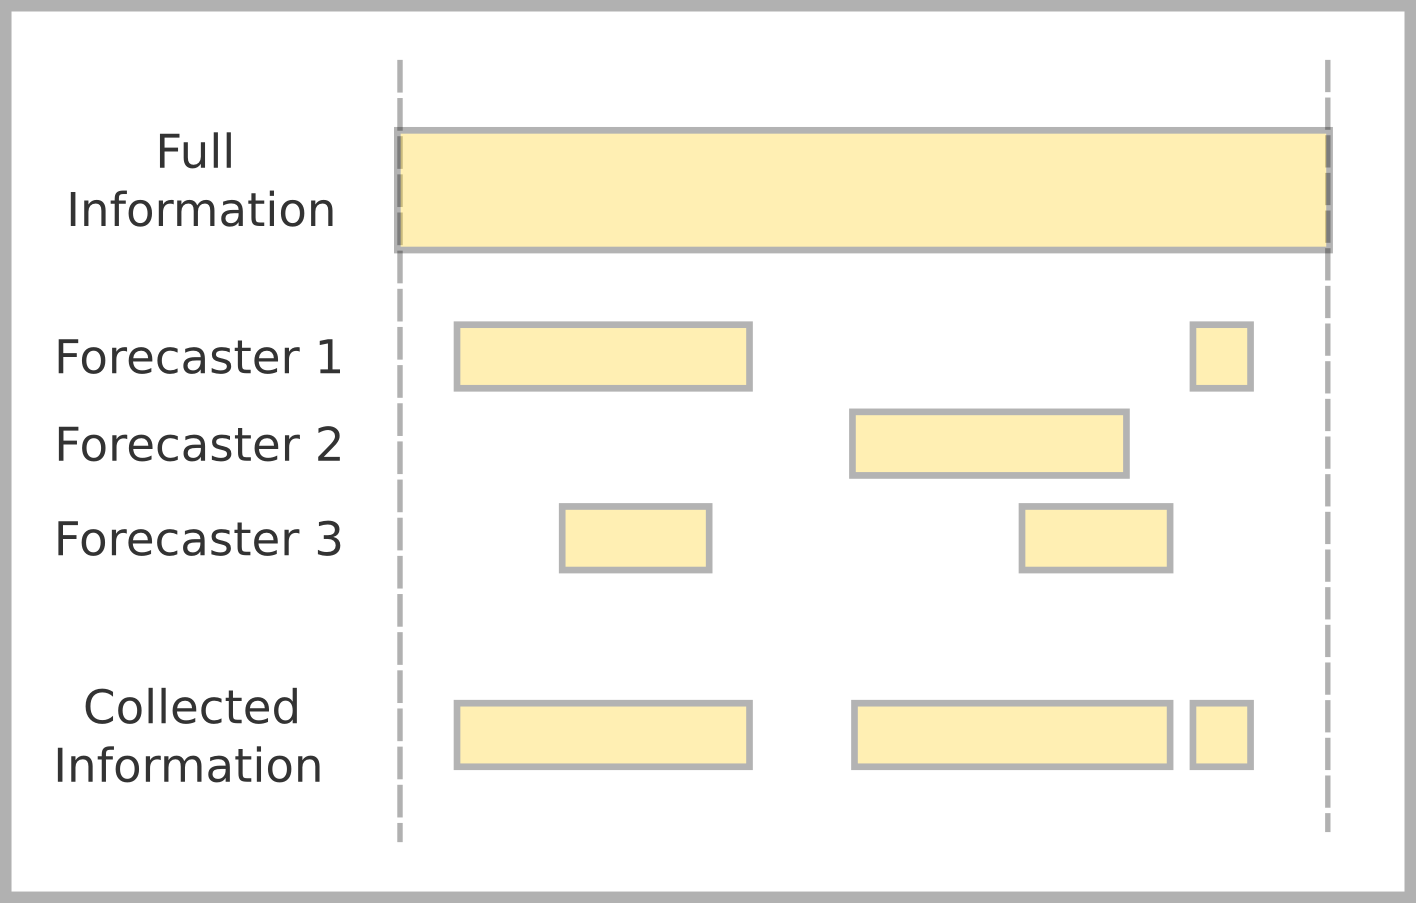
\includegraphics[width = 0.5\textwidth]{N=N.png} % requires the graphicx package
%   \caption{Illustration of information under $N=3$ forecasters. The top bar represents $\F$ that contains all possible information that can be known about $Y$. Horizontally aligned with Forecaster $j$ is the partial information $\F_j$ revealed by that forecaster. The revealed information $\F''$ is the union of the forecasters' partial information sets.}
%   \label{CollectInfo}
%\end{figure}


%\marginpar{This figure is not precise. That is not the revealed information. It is the oracle information.}

%\marginpar{This equality must be made a.s.}

\begin{class}[Efficiency]\label{infoAgg}
An aggregator $\mathcal{X}$ is efficient if there exists a probability space $(\Omega, \F, \P)$ under which $\mathcal{X} = \E(Y | X_1, \dots, X_N)$ a.s. or, equivalently, $\mathcal{X} = \E(Y | \F'')$ a.s. with $\F'' = \sigma(X_1, \dots, X_N)$. Denote all efficient aggregators with $\mathcal{X}''$. 
%Sometimes $\mathcal{X}''$ is called the revealed aggregator because it uses all the information that the forecasters' reveal through their predictions. 
%Suppose the outcome $Y$ and its predictions $X_j$, for $j = 1, \dots, N$, are defined on some probability space $(\Omega, \F, \P)$. Under this space, the \textit{revealed aggregator} is defined as the conditional expectation $\mathcal{X}'' := \E(Y | \F'') = \E(Y | X_1, \dots, X_N)$. This aggregator represents the forecasters' combined information   and hence is said to collect information. 
\end{class}
%, namely the $\sigma$-field generated by the individual predictions. 
 %This prediction is called the \textit{revealed
%aggregator} because it uses all the information that the
%forecasters' reveal through their predictions.  In fact, by the uniqueness of conditional expectation, it is the only aggregator that performs such information collection.
%Even though
%$\mathcal{X}'' $ is typically too abstract to be applied in practice,
%it provides an optimal baseline for aggregation
%efficiency. 
%Therefore it provides an ideal benchmark for
%understanding aggregators currently used in practice. 
\noindent

In regression analysis $\mathcal{X}''$ is known as the \textit{regression function} and is often considered the \textit{best predictor} of $Y$ (see, e.g., \citealt[Theorem 6.3.1]{christensen2011plane}) because it minimizes the expected Bregman loss \citep{satopaamodeling2}. 
%For this reason, most regression procedures aim to find or estimate $\mathcal{X}''$. 
%The goal of most predictive procedures is then to find or estimate $\mathcal{X}''$. 
%\marginpar{This is the best aggregator now matter what kind of variation there is. Assume that variation is entirely from information and show that measures of central tendency do not work}
%Observe that each $\mathcal{X}''$ is paired with a probability space under which it is efficient. 
%\cite{dawid1995coherent} call such pairs \textit{compatible} and give some results on how to construct one from the other. Our focus, however, is not on any specific pair. Instead 
%This paper does not focus on estimating $\mathcal{X}''$ but instead investigates whether there exists a probability space under which some popoular aggregator, such as the weighted average or the median, is efficient. If there is not, then this aggregator will always be \textit{inefficient} and hence can be improved upon. 
%Unfortunately, showing these kinds of inefficiency results directly with Definition \ref{infoAgg} can be challenging. A more natural approach is to find common properties of all efficient aggregators. This then gives a ``toolbox'' for checking whether any given aggregator can be efficient or not.
% like an efficient aggregator.  
% because it does not use the forecasters' combined information under any probability space.
% under which it would use all the forecasters' information. 
%In this paper an aggregator is said to collect information if and only if it is a member of class described by Definition \ref{infoAgg}. 
%First, however, it is necessary to understand the common behavior of the efficient aggregators. This is given in the 
%following theorem that
%In order to better understand efficient aggregators, the next theorem
Unfortunately, Definition \ref{infoAgg} is rather abstract and does not render itself well to analysis. In response, the next theorem fully characterizes efficient aggregators in terms of two necessary and sufficient properties. 
% At this level $\mathcal{X}''$ is very abstract and clearly cannot be applied in practice. Fortunately, however, its properties can be studied. 
%  These are summarized in the following theorem. 
These properties form a ``toolbox'' for 
%understanding how a given aggregator processes information. 
%In particular, an uncalibrated aggregator is not based on any information set about $Y$ and hence must distort the forecasters' information. A calibrated but non-expanding aggregator, on the other hand, uses only a subset of the forecasters' information. 
showing that some aggregator is not efficient.
% in the sense described in Definition \ref{infoAgg}. 
%This definition describes a weak form of efficiency: there is some probability space under which the aggregator is efficient. On the flip side, 
In particular, violating any of the properties shows a strong form of inefficiency: there is no probability space under which the aggregator is efficient. The proofs of this and all other theorems are deferred to the Appendix.
%This is the type of inefficiency that we will prove for different class of aggregators. 


%\marginpar{Be careful as this holds only if the assumptions hold}

  

%\marginpar{What do we mean by "collect information" and does not collect information. Need a picture. Brain analogy}

%WRITE OUT A CLASS OF AGGREGATORS HERE AND EXPLAIN THAT IT DEPENDS ON THE PROBABLITY SPACE. THAT IS, A SPECIFIC INSTANCE OF X'' COLLECTS INFORMATION UNDER A CERTAIN PROBALITY SPACE. 
%\marginpar{Explain that X'' really coincides with the maximizing sharpness subject to calibration. It is the limit. }

%\marginpar{If one has a model, why cannot one just directly compute the $X''$ by taking the expectation. This leads to the curse of dimensionality. }

%COLLECTS INFOMRATION IF AND ONLYF IF IT IS EQUAL TO X'' FOR SOME PROBABLITY MODEL. 

%\marginpar{We do not need marginal consistency here as it is implied by calirbation. Can mention this afterwards.}

\begin{theorem} \label{optimal}
%Suppose that $X_j = \E(Y | X_j)$ for all $j = 1, \dots, N$ and denote the revealed aggregator with $\mathcal{X}'' = \E(Y | \F'')$, where $\F'' = \sigma(X_1, \dots, X_N)$. 
%The individual predictions agree with $Y$ in expectation, that is, $\E(X_j) = \E(Y) = \mu_0$. 
%Let $\delta_{max} := \max_j \{ \Var(X_j)  \}$ be the maximal variance among the individual prediction.
% $\delta_{max} = \E[(\mu_0 - X_j)^2]$. 
An aggregator $\mathcal{X}$ of calibrated predictions $X_1, \dots, X_N$ is efficient if and only if it has the following two properties.
% All efficient aggregators $\mathcal{X}''$ have the following properties. 
\begin{enumerate}[(i)] \label{properties}
%\item  $\mathcal{X}''$ is invariant to invertible transformations of the predictions: if $f(\cdot)$ is an invertible transformation, then $\mathcal{X}'' = \E(Y|X_1, \dots, X_N) = \E(Y | f(X_1), \dots, f(X_N))$. 
%\item $\mathcal{X}''$ is \textit{marginally consistent}:  $\E(\mathcal{X}'') = \E(Y) =  \mu_0$. \label{margEfficient}
\item $\mathcal{X}$ is \textit{calibrated}: $\E(Y|\mathcal{X}) = \mathcal{X}$ a.s. \label{calibrationEfficient}
\item $\mathcal{X}$ is \textit{extremizing}: $\Var\left[ \E(Y | X_j,  j \in \v)\right] \leq \Var(\mathcal{X})$ for all  subsets $\v \subseteq \{1, \dots, N\}$. \label{expandEfficient}
%$\max ( \Var(X_1), \dots, \Var(X_N)  ) \leq \Var(\mathcal{X})$. 
%In words, the variance of $\mathcal{X}''$ is always at least as large as that of the most variable prediction. 
%\item \textbf{Information Collection.} $\mathcal{X}''$  is the only aggregator that uses all the information contained in the predictions $X_1, \dots, X_N$. In other words, $\mathcal{X}''$ is the only aggregator that collects information. 
%\item $\mathcal{X}''$ is the aggregator that minimizes the expected Bregman loss, such as the quadratic loss \citep{satopaamodeling2}.
%value of a large class of loss functions, including the quadratic loss \citep{satopaamodeling2}. 
\end{enumerate}
\end{theorem}
%Marginal consistency states that the prediction and the outcome agree in expectation.
%According to item ii), $\mathcal{X}''$ is calibrated. Given that  $\mathcal{X}''$ is based on $\F''$, this property follows directly from the fact that a prediction is calibrated if and only if it is based on some information set \citep{satopaamodeling}. 
% or, equivalently, based on some information set about $Y$. 
% Intuitively, this should be expected from an information collector. 
Item (\ref{calibrationEfficient}) does not require calibrated predictions. In fact, an efficient aggregator, like any conditional expectation, is always calibrated. Given that $\mathcal{X}''$ is calibrated, it is also marginally consistent: $\E(\mathcal{X}'') = \E(Y) = \mu_0$. To see this, consider a calibrated prediction $X$. Then $\E(X) = \E[\E(Y|X)] = \E(Y) = \mu_0$. Consequently, all calibrated predictions (individual or aggregate) are marginally consistent. The converse, however, is not true. For instance, Theorem \ref{contraction} shows that any non-trivial arithmetic mean is marginally consistent but not calibrated. This is an important observation because it provides a technique for proving lack of calibration (and hence inefficiency) via marginal inconsistency -- a task that can be much easier than proving lack of calibration directly. 
%To illustrate, the technique quickly shows that a linear aggregator $\sum_{j=1}^N \beta_j X_j$ with $\beta_j \in \mathbb{R}$ and  $\sum_{j=1}^N\beta_j \neq 1$ is not calibrated or efficient as long as $\mu_0 \neq 0$ because $\E \left( \sum_{j=1}^N \beta_j X_j \right) =  \sum_{j=1}^N \beta_j \E\left( X_j \right) =  \mu_0 \sum_{j=1}^N \beta_j  \neq \mu_0.$ This class of aggregators, however, is not a subset of means. Therefore it is not discussed further in this article. 
% In fact, the proof of Theorem \ref{contractionXphi} makes use of this shortcut. 


%\marginpar{In Bayesian statistics this is nothing but the posterior expectation of the outcome.}


%\marginpar{Which parts rely on calibration and which dont.}


%\marginpar{Theorem: $X''$ is the only aggregator that collects information.}
%\marginpar{Explain how to calibrate predictions based on $\P$.}

Item (\ref{expandEfficient}), on the other hand, requires calibrated predictions. 
To interpret this property, suppose the forecasters' information sets form an increasing sequence
%Proposition \ref{calibrationProp} combined with the fact that conditional expectation contracts in $L^2$ \citep[Theorem 5.1.4.]{durrett2010probability} show that the variance of any calibrated prediction (individual or aggregate) is upper-bounded by $\Var(Y)$. 
%%This follows directly from the fact that each reliable prediction can be associated with a sub-$\sigma$-field and the fact that conditional expectation is a contraction in $L^2$ \citep[Theorem 5.1.4.]{durrett2010probability}. 
%Theorem \ref{optimal} then shows that the corresponding lower bound for $\Var(\mathcal{X}'')$ is the maximum variance among the forecasters. More generally, consider 
%the least informative sub-$\sigma$-field, namely the trivial $\sigma$-field $\F_0 := \{\emptyset, \Omega\}$. A prediction based on $\F_0$ is always equal to the marginal mean $\mu_0$ and hence has zero variance. On the other hand, a prediction based on all the information, namely the principal $\sigma$-field $\F$, is equal to $Y$ and hence has variance $\Var(Y)$. 
%The intermediate cases can be understood by considering 
%an increasing sequence of $\sigma$-fields 
$\{\emptyset, \Omega\} = \F_0  \subseteq \F_1 \subseteq \dots \subseteq \F_N \subseteq \F$.  Note that $\E(Y|\F_0) = \mu_0$ and $\E(Y|\F) = Y$. \citet{satopaamodeling2} show that the variances of these predictions would follow the same order as their nested information sets, that is, $0 = \Var(X_0) \leq \Var(X_1) \leq \dots \leq \Var(X_N) \leq \Var(Y) = \delta_0$. Thus the informativeness of a calibrated prediction is proportional to its variance. Naturally, if an aggregator is efficient, it uses all of the forecasters' information and hence at least as much information as any subgroup of these individuals. Therefore $\mathcal{X}''$ is necessarily at least as variable as every individual prediction or, more generally, the efficient aggregate of any subset of them. 
%This outward tendency is our first hint that that means may not be efficient. 
This is precisely what item  (\ref{expandEfficient}) describes. 
%The final item iv) shows that $\mathcal{X}''$ is the optimal aggregator under a large class of different loss functions and hence justifies efficiency as a goal in forecast aggregation. 
%This was proven in \cite{satopaamodeling2}.
%This is a necessary condition for an aggregator to be a collector of information.
% Therefore any aggregator that \textit{expands} variance and satisfies this condition is
%%because it is expected to deviate more from the marginal mean than any of the individual predictions. This is a necessary condition for an aggregator to be 
%considered a collector of information. 

%\marginpar{Do we want to discuss the coherence idea somewhere}

%If variance represents the amount of information, then a reasonable goal in aggregation is to maximize variance subject to calibration. Previously this goal has been well-established in the probability forecasting literature \citep{murphy1987general, gneiting2007probabilistic}. There a calibrated and highly variable prediction  is
%very useful to the policy-maker because it is both accurate and close
%to the most confident values of zero and one. Of course, no aggregator can use more information than $\F''$. Therefore a calibrated aggregator cannot be more variable than $\mathcal{X}''$. As a result, the general goal of maximizing variance subject to calibration is equivalent to aiming to be as close to $\mathcal{X}''$ as possible. Item iv) recasts this goal in terms of minimizing a class of loss functions. 

%%Overall, this discussion poses an interesting hypothesis: 
%%does Definition \ref{infoAgg} contain any measure of central tendency? 

%% may then end up having a too low variance and hence be inefficient. 
%To illustrate, suppose that all the intelligent analysts independently predict a probability of $0.9$ that Bin Laden is in the compound. If these predictions are based on somewhat different information, then their combined information should lead to an aggregate greater than $0.9$. In this simple scenario, however, all measures of central tendency aggregate to $0.9$. Therefore they are not using the forecasters' information efficiently. Even though this is admittedly a very contrived example, it does suggest an interesting question: are measures of central tendency inherently inefficient in aggregating information-driven predictions?
%%They do not account for the information heterogeneity among the forecasters and hence cannot collect their information. 
%%%In fact, \cite{satopaamodeling} explain that averaging-like techniques work well when the individual forecasters have very similar sets of information, that is, when there really is no information aggregation problem to begin with.
%%Instead, they reduce ``measurement error,'' which is philosophically very different to the idea of information aggregation discussed in this paper. 
%This question is explored more rigorously in the next section. 

% Past literature has acknowledged this but has typically worded it as maximizing sharpness subject to calibration. Here sharpness measures how far the predictions are from the naive baseline prediction $\mu_0$. 
%
%They
% explain how the quality of a probability forecast
%(individual or aggregate) is typically measured in terms of
%\textit{reliability} and \textit{resolution} (sometimes also known as calibration and
%sharpness, respectively). Reliability describes how closely the
%conditional event frequencies align with the forecast
%probabilities. Resolution, on the other hand, measures how far the
%predictions are from the naive baseline forecast, that is, the marginal
%event frequency. A prediction that is reliable and highly resolute is
%very useful to the policy-maker because it is both accurate and close
%to the most confident values of zero and one. Therefore a
%well-established goal in probability forecasting is to maximize resolution subject to
%reliability \citep{murphy1987general, gneiting2007probabilistic}.
%
%
%Recall that in probability forecasting a well-established goal is to maximize resolution subject to reliability. This goal can be easily interpreted intuitively with the help of partial information. First, conditioning on reliability requires the prediction to be consistent with some set of information about $Y$. Maximizing the resolution of this prediction takes it as far from $\mu_0$ as possible. This is equivalent to increasing the variance of the prediction as close to the theoretical upper bound $\Var(Y)$ as possible. Therefore the goal is equivalent to maximizing the amount of information that the prediction is consistent with. Intuitively, this is very reasonable and should be considered as the general goal in forecasting.


%\subsection{Weight Functions}
%This section explores what we really know about the weight functions. These functions input the predictions $X_1, \dots, X_N$. However, given that each of these predictions is a function of $Y$, the weights can be also considered to be functions of $Y$ and the forecasters' information sets. This can be a bit confusing however because the weight function does not apply the information set in anything but the conditional expectation. Hence it may be clearer to just think about these weight functions as functions of the predictions. 
%\begin{enumerate}
%\item If $\E \sum_j w_j X_j = \mu_0$, then $\sum_j \Cov(w_j,X_j) = 0$. 
%\item $\sum_j w_j = 1$
%\item 
%\end{enumerate}

%\marginpar{We must explain somewhere why we care about the random weighted average; show with examples that this includes many of the averages such as the geometric mean, etc.  This captues the General Mean function for a finite t; see Steele's book}
%
%
%"The challenge is to identify ways to extract the maximum amount of predictive informa- tion form judgment and to us this information effectively to improve prediction accuracy" Nada Sanders and Larry Ritzman in Judgmental Adjustments of Statistical predictions. 


%In particular, if a given aggregator violates any of these properties, it does not fall within Definition \ref{infoAgg}. This suggests a \textit{strong} form of inefficiency: it is impossible to construct a probability space under which the given aggregator is efficient. 
%From now onwards inefficiency is taken to entail this strong form. 


%Unfortunately, showing these kinds of inefficiency results directly with Definition \ref{infoAgg} can be challenging. A more natural approach is to find common properties of all efficient aggregators. This then gives a ``toolbox'' for checking whether any given aggregator can be efficient or not.






\subsection{Literature Review}\label{Lit Review}
%Today's literature on forecast aggregation is vast and spans several fields including psychology, statistics, management science, operations research, and others. 
%The seminal paper in forecast aggregation is often considered to be \cite{bates1969combination}. In this work the authors discuss different ways to weigh and average two predictions of airline passenger data.
%%% for combining two forecats 
%%%% is often considered as the seminal paper. 
%%%%Two decades after the seminal forecast aggregation paper \citep{bates1969combination}, 
%%%Two decades after writing this paper, 
%In 1989 Nobel laureate C. W. J. Granger emphasized the importance of forecasters' information in both theory and interpretation of predictions \citep{granger1989invited}. 
%%Much later, \cite{satopaamodeling} showed that optimal aggregation is not well-defined if the model does not incorporate forecasters' information. 
%%The general idea is that typically it is not possible to determine ex-ante which forecaster will be the most accurate, and even if this could be done, 
%%To illustrate,
%% For instance, Leon Panetta should combine the predictions in a way that utilizes all the information among the intelligence analysts. 
%%\marginpar{The aggregator must collect info under the specific model that incorporates information sets. This is all model specific.}
%%\marginpar{Also cannot double count all the public information; should use and take into account all information only once. This bias is known as shared-information bias}
%%\marginpar{Perhaps we want a picture here to illustrate the complexity of information collection. Similarly to what Palley had but high light the outer rim, }
%%After all, forecasting should be based on information about the future outcome -- not on instinct, random guessing, or gut feel. 
%This led to different models of calibrated predictions. 
% inherent link between forecasting and information led to several stylized models of information-driven predictions.
%These models typically treat the outcome as a random variable and each prediction as a different expectation of this outcome, conditioned on the forecaster's information. 
%The main modeling differences are in the assumptions made about the structure of the forecasters' information.

%\marginpar{Many infomration models but they tend to be so called generated signals. Cite Scott here and explain this incudes a very particular structure on the information driven predictions. Not realistic. Better to work with full generality.}


One of the earliest inefficiency results is by Nobel laureate C. W. J. Granger who emphasized the importance of forecasters' information in both theory and interpretation of predictions \citep{granger1989invited}. He shows that the equally weighted arithmetic mean is an inefficient aggregator of calibrated predictions if each forecaster's information consists in equal parts of shared and private information. Later on, \cite{kim2001inefficiency} reached the same conclusion. 

%\marginpar{Check if these truly are info models -- or are they measurement error models}

%In 1989 After all, principled forecasting should stem from true information -- not from intuition, gut feel, or good luck. This suggests that multiple predictions should be combined into a consensus that captures as much of the individuals' true information as possible. 


Real-world forecasters, however, can have different amounts of information, and not all information is either completely shared or private. For instance, two forecasters may share information that a third forecaster does not know and so on. 
% Therefore different parts of information can be shared by different subgroups of the forecasters, and 
This way the forecasters' information can be seen to form a complex structure of partially overlapping sets. 
% \cite{figlewski1983rational} analyze a model that groups the forecasters into two types, depending on their information. 
% Both authors
% The result was named the \textit{inefficiency of the means}. 
% and hence can be improved upon. 
% This result became known as the \textit{inefficiency of the means}. 
%The main limitation of this work stems from its restrictive assumptions on the forecasters' information structure: all information is known either by everyone or by only one forecaster. Due to its tractability, this \textit{symmetric} information model has become the popular choice in the literature (see, e.g., \citealt{ottaviani2006strategy, lichtendahl2013wisdom, palley2015eliciting}).

%\marginpar{This is not general enough to be called that. Means is defined as etc. Cite and then explain that it really is inefficency of strict means. }

%, it does not imply the strong form of inefficiency discussed in Section \ref{InfoCollection}.
%that averaging is always inefficient. 
  

  
  
%Unfortunately, this is somewhat of a misnomer because their result only applies to the equally weighted arithmetic mean under specific models and structural assumptions on the forecasters' information. 
%All these authors make heavy structural assumptions on the forecasters' information. 

%\marginpar{Be nicer}
%Therefore extrapolating to a strong form of inefficiency (see Section \ref{InfoCollection}) from their isolated instances would be similar to declaring all means inefficient based on the simple doctor-example given in the introduction. Both conclusions would be clearly unjustified.
% To truly claim inefficiency of the means, the analysis must cover all means and not rely on any particular probability model or information structure.
%under all models of 
%information-driven predictions.
% and
% \cite{granger1989invited} and \cite{kim2001inefficiency} also make strict structural assumptions on the forecasters' information.
%The analysis should also 
%not constrain the forecasters' information in any way.
%Even though such an analysis may appear combinatorially intractable,
%%Previous work, however, has shown this to not be the case.
%%Some authors, however, have succeeded in this.
%% shown that this is not the case. 
%%In fact, some authors have analyzed the average prediction without restricting the forecasters' information structure. 
%%This, however, is not the case.
%some progress has been made. 
%Some authors have analyzed aggregation without constraining the information structure.
By operating under the partial information framework, it is possible to analyze aggregation without constraining the information structure. Some previous authors have done exactly this. In particular, \cite{dawid1995coherent} show that the weighted arithmetic mean of two calibrated predictions of a binary outcome is always inefficient as long as one forecaster does not know everything that the other forecaster knows.
%This result, however, is not directly useful for many real-world forecasting applications because these often involve a large number of forecasters.
This result was later on extended to $N \geq 2$
%\cite{hora2004probability} first extended the result to two 
calibrated predictions of a binary outcome \citep{hora2004probability, Ranjan08, gneiting2013combining}. 
%All these works treat the weights as fixed and hence do not apply to other measures of central tendency such as the median.
%, and \cite{Ranjan08} and \cite{gneiting2013combining} extend the result to $N \geq 2$ calibrated probability predictions. 
%To the best of our knowledge, their result is currently the most general one in this area. 

%Possibly because of the heavy focus on probabilistic predictions, the inefficiency of (arithmetic) means is sometimes believed to be limited to calibrated probability predictions \citep{jose2013trimmed}. 
Some attempts have been made for an even more general result. For instance,  \cite{parunak2013characterizing} suppose that all forecasters know equally much and that not all information about a binary outcome can be known. They then consider an omniscient prediction that optimally uses all information that could possibly be known. They illustrate that this prediction can be outside the the convex hull of the individual calibrated predictions. The omniscient prediction, however, is not an aggregator as it is not a function of the predictions (or measurable with respect to $\F''$). Furthermore, it is always based on at least as much (and often more) information than the individual predictions combined. 
% In fact, if it is based on $\G \subseteq \F$, then $\F'' \subseteq \G$.  
%it uses an information set $\G 
% it is not measurable with respect to $\F''$. 
%Instead it is the prediction made by an ``all-knowing'' forecaster. 
% It may contain information unknown to all forecasters, and even if the forecasters' information did cover all of $\G$, it is unlikely that $\G$ can be recovered from the predictions such that $\G = \sigma(X_1, \dots, X_N)$.
Therefore it is not clear how directly these results relate to forecast aggregation. Their work, however, did inspire us to look for a general inefficiency result. 
  
% \marginpar{This, however, gives us inspriation to work towards a general result. Twise this positively.} 
  
  

%\marginpar{Must make it crystal clear what is ours and what is theirs.}

%\marginpar{They only consider fixed weights. Weights cannot depend on the realised values of the predictions. In practice thought one may observe the predictions and then decide how to aggregate them. Seems completely reasonable. This limits the application context to a setting where the weights can be somehow determined before hand. In real life, howver, the aggregatort may eamine the predictions and then decide etc. }

%Unfortunately, their results leave much unanswered about scope and root cause of the inefficiency. For one, it is unclear whether the inefficiency is particular to weighted arithmetic means of probability predictions, or whether the phenomenon is more widely spread than that. 
%It is unclear whether the inefficiency stems from weighted averaging or perhaps just to combining probability predictions of a binary outcome. 
%This is the current state of the literature. In other words, to the best of our knowledge, the most general result in this line of research shows that the weighted average of calibrated probability predictions of a binary outcome is inefficient. 
%These authors also make no assumptions about the underlying probability model. 
%Therefore the results are very general. 
%Even though these authors do not focus on the role of information, their forecasters can be shown to be operating on different information sets. The structure of these information sets, however, is in no way restricted.  Instead the results are derived jointly under all possible information structures. 
%In addition to not restricting the information structure,
%These results are highly general not only because they consider all possible information structures but also because they do not assume anything about the joint distribution of the outcome and its information-driven predictions. 
%The only assumption is that the outcome and the predictions operate under a common probability model.
%Unfortunately, none of these analyses provides strong intuition for the source of inefficiency. Therefore, to the best of our knowledge, our analysis is the first to explain the inefficiency of the means in intuitive terms.  

%\marginpar{Maybe it is all about probablity predictions that estimate something on the border of the space. This, however, is not so with the CDF valued predictions. }

%\marginpar{These are merely results that do not discuss the sources much.}
%
%\marginpar{A real proof is missing}

%\cite{parunak2013characterizing} suppose that the final outcome is determined by a finite sum of i.i.d. Bernoulli random variables. Only $M$ of these values are available to the forecasters. Each forecaster then makes a calibrated probability prediction based on some $K < M$ available values.
%% probability predictions that are based on (equally large) subsets of some available partial information $\G \subseteq \F$. They
%The authors explain that if there are at least $K$ more ones than zeros among the available values, then the prediction based on all $M$ available values can be outside the convex hull of the individual predictions. Unfortunately, this optimal prediction is not an aggregator as it is not measurable with respect to $\F''$. 
%%They use this observation to draw general conclusions about optimal aggregation. $\E(Y|\G)$, however, is not an aggregator. In fact, it is not even a function of the predictions. 
%Instead it is the prediction made by an ``all-knowing'' forecaster. 
%% It may contain information unknown to all forecasters, and even if the forecasters' information did cover all of $\G$, it is unlikely that $\G$ can be recovered from the predictions such that $\G = \sigma(X_1, \dots, X_N)$.
%  Therefore it is not clear how their results apply to aggregation. 
 
% \marginpar{No work considers noisy predictions}
 
In summary, existing general inefficiency results concern the weighted arithmetic mean of calibrated predictions of a binary outcome. The weights are considered fixed ex-ante before the predictions are observed, and therefore the results do not apply to many common means such as the median or trimmed means. The discussion has also remained rather technical with no attempt to explain the reason or phenomenon behind the inefficiency. This may be because information has not been recognized as the driver of differences in calibrated predictions. Instead, the authors have mostly worked directly with the definition of calibration. Even though this is equivalent to Assumption \ref{assumption2}, it is less intuitive  and hence does not point as directly towards the core reasons behind the inefficiency.
 
% \marginpar{Move this up; explain up that the others use calibration to analyze all info structures. Then can be shortened here.}
%  incompatibility of the means and calibrated predictions. 


 
Part of our goal now is to settle this general conversation around inefficiency. First, we show that the inefficiency is not limited to the arithmetic mean of calibrated  predictions of a binary outcome but instead applies to almost all  means of calibrated predictions of any type of (univariate) outcome.
% Thus, even the arithmetic mean with weights determined ex-post is almost never efficient.
  Second, we intuitively explain the reasons behind this inefficiency. Third, to the best of our knowledge, we are the first to discuss the inefficiency of the means in the context of uncalibrated predictions. 


%we study aggregation inefficiency in the context of non-calibrated predictions. We are not aware of any previous inefficiency results regarding aggregation of non-calibrated predictions.

%Our work now hopes to conclude this line of research by
%More specifically, we show that the inefficiency arises when a (strict) mean is applied to any type of calibrated predictions of a univariate outcome. We hope to clarify the broader phenomenon behind the aforementioned articles  by explaining that calibrated predictions and means are incompatible concepts. An aggregator operates under some assumptions about the observed variability in the predictions. Loosely speaking, means interpret variation as noise and aim to reduce it to capture some central value that the forecasters are trying to predict or measure. All variation in calibrated predictions, however, is caused by differences in the forecasters' information. In other words, variation in calibrated predictions signals information -- not noise. The means then misinterpret the variability and lead to a suboptimal aggregate.

%Loosely speaking, 
%
%The means are designed to reduce noise in the observations -- not to collect information. 
%
%
%
%
%in a sense that they do not come from the same probability model. This is crucial because the probability model specifies how the predictions translate into information about the outcome. Thus, if the aggregator and predictions are incompatible, the aggregator misinterprets the predictions and is likely to give a nonsensical answer. 
% means apply an incorrect translation to information-driven predictions and hence remain inefficient. 
%%fail to be efficient in aggregating information-driven predictions. 
%
%\marginpar{We do actually conclude the inefficiency of the means section. These are all means defined as within the convex hull. Define means as Cauchy did: all functions that are within the convex hull of the predictions. See p. 13 of Aggregation Functions Part Means; most general definition of the mean we know of. }

%\marginpar{Sometimes this inefficiency or lack of calibration is assumed to persist only for weighted aveeraging of probabilty predictions. However, this is not true.  Cite Yael's paper. She specifically says "in point forecasting, the simple average is a good forecast" See the beginning of the paper.}


%\marginpar{Many papers written with one result after another. We are hoping now to provide some clarity to this issue as a whole. We are trying to explain the wider phenomeno that is happening.}

% arises because measures of central tendency and information-driven predictions do not come from the same probability model. If an aggregator and the predictions do not come from the same model, the aggregator cannot 

% do not operate under the same model as information-driven predictions. 
%is not limited to probability predictions or weighted averaging but instead 
%is not limited to probability predictions or averaging but instead of 


%not caused by the type of outcome and that it holds under a much larger class of aggregators, namely the measures of central tendency. This way the story about inefficiency evolves to one of central tendency and information driven predictions. 
%These two concepts are incompatible and hence should not be used together because they arise from very different assumptions of the underlying model. 


%Lastly, unlike previous results, we do not focus on binary outcomes but instead show that inefficiency persists despite the outcome type. 


%\marginpar{this needs a powerful sentence making it clear what we are ending the story. We generlaize to any type and to any measure of central tendency}

%\marginpar{Must make it clear that we are considering univariate predictions}

%\marginpar{We explain that the story is not specific about probability predictions or weighted averaging. Instead the story is much more general than that. In fact, despite the outcome, the story is about central tendency. Make this seems much more general!}

%\marginpar{What are we saying here: The inefficiency is not inherent to averaging. It is about central tendency; can't escape the convex hull. In fact, some weighted averages in some simple examples may not qualify as random strict convex combos. We show that story is not about weighted averges but about central tendency}

%\marginpar{We have to cite Scott's paper..}

%\section{MEASURES OF CENTRAL TENDENCY} \label{MeasuresOfCentralTendency}
\section{AGGREGATING CALIBRATED PREDICTIONS} \label{MeasuresOfCentralTendency}


%\marginpar{Write this as fixed weights and then later on random weights}

%\subsection{Weighted Averages} \label{contractionSection}
\subsection{Arithmetic Mean} \label{contractionSection}

%EPLAIN HERE THAT AVERAGING THE NONCALIBRATED IS NOT THE SAME AS AVERAGING THE CALIBRATED. HOWEVER, BUDESCU SHOW THAT CALIBRATING FIRST AND THEN AVERAGING INCREASES PERFORMANCE. 
%
%``An equal-weights rule offers a
%reasonable starting point, and a trimmed mean is desirable if you combine predictions resulting
%from five or more methods. Use different weights if you have good domain knowledge or
%information on which method should be most accurate." Armstrong
%
%weights can be determined by Newbold and Granger 1974
%
%
%WRITE AS BOLD AGGREGATOR CLASS 1: EXPLAIN WHAT WEIGHTED AVERAGE IS. 

%This section generalizes the analysis by \cite{dawid1995coherent} and \cite{Ranjan08} of the weighted average.

The (weighted) arithmetic mean is the most common way to combine predictions in practice \citep{hora2004probability, Ranjan08, jose2013trimmed}. In fact, this practice is so common that sometimes ``combining predictions'' is taken to mean ``averaging predictions'' \citep{armstrong2001combining}. 
%In fact, even some more complex aggregators often incorporate is as a sub-component (see Section \ref{TranscontractionSection}).
% In practice most aggregators rely the weighted average of the individual predictions.
  Therefore it is a natural starting point for our analysis of the means. 
  The arithmetic mean is defined and notated as follows.
% More precisely, the focus is on the following class of aggregators.
\begin{class}[Arithmetic Mean] \label{Xw}
An arithmetic mean is $\mathcal{X}_w := \sum_{j=1}^N w_jX_j$, where each weight $w_j \geq 0$ is fixed and $\sum_{j=1}^N w_j = 1$. It is non-trivial if there exists a  pair $i \neq j$ such that $\P(X_i \neq X_j) > 0$ and $w_i, w_j > 0$.
\end{class}
%The following theorem shows that a non-trivial weighted average is neither expanding nor calibrated. Therefore it is ne can be considered suboptimal.
%The most famous member of this class is the equally weighted average $\frac{1}{N}\sum_{j=1}^N X_j$ that sets all $w_j = 1/N$. 
Similarly to the previous studies mentioned in Section \ref{Lit Review}, the weights here cannot depend on the realized values of the predictions. Instead, they must be fixed before the predictions are observed. Unequal weights can be justified based on additional information such as the forecasters' self-reported expertise in the given prediction task or past prediction accuracy of the forecasters. 


The non-triviality condition, on the other hand, ensures that $\mathcal{X}_w$ does not assign all weight to a single prediction (or a group of a.s. identical predictions) but instead attempts to combine information from multiple different sources. Therefore, given that our goal is to analyze and understand aggregation of information from different sources, the discussion can safely focus only on the non-trivial cases.
% $\mathcal{X}_w$ to be non-trivial without losing any generality. 
That being said, the next theorem describes a non-trivial $\mathcal{X}_w$ in the light of the efficiency properties of Theorem \ref{optimal}. 
%Note that any deviation from those properties indicates inefficiency. 
% The proof is again deferred to the Appendix. 

%\marginpar{Important to note that the weights have to be fixed.}
%\marginpar{Non-trivilality is a bit more than this. If one uses a subset of the others information it will be different but weight one must be assigned for efficiency. Therefore non-triviality suggests cases where information must be gathered from different sources for efficiency.}
%\marginpar{It does not hold under all probability spaces as A1 and A2 must be satisfied.}

\begin{theorem}\label{contraction}
%Suppose that $X_j = \E(Y | X_j)$ for $j = 1, \dots, N$.  
%Let $m = \argmax_j  \Var(X_j) $ identify the prediction with the maximal variance; that is, $\Var(X_j) \leq \Var(X_m)$ for all $j = 1, \dots, N$. 
% $\delta_{max} = Var(X_m)$.  
 If $\mathcal{X}_w$ is non-trivial, then the following holds.
%  under all probability spaces $(\Omega, \F, \P)$.
%Then the following holds.
\begin{enumerate}[(i)]
\item  $\mathcal{X}_w$ is marginally consistent: $\E(\mathcal{X}_w) = \E(Y) = \mu_0$. 

\item $\mathcal{X}_w$ is not calibrated: $\P\left[\E(Y | \mathcal{X}_w) \neq \mathcal{X}_w\right] > 0$.
% if there exists a prediction pair $i \neq j$ such that $\P(X_i \neq X_j) > 0$ and $w_i, w_j > 0$. In words, $\mathcal{X}_w$ is necessarily uncalibrated if it assigns positive weight to at least two different predictions.  
\label{XwCalib}
%Given that predictions are random variables, any two predictions, $X_i$ and $X_j$, are considered different if and only if $\P(X_i \neq X_j) > 0$.
  
 \item The variance $\Var(\mathcal{X}_w)$ is too low. More specifically, if $\mathcal{X}_w'' :=  \E(Y| \mathcal{X}_w)$ is the calibrated version of $\mathcal{X}_w$, then $\E(\mathcal{X}_w) = \E(\mathcal{X}_w'') = \mu_0$ but $\Var(\mathcal{X}_w) < \Var(\mathcal{X}_w'')$. In other words, $\mathcal{X}_w$ is under-confident in a sense that it is, in expectation, closer to the marginal mean $\mu_0$ than its calibrated version $\mathcal{X}_w''$ is. \label{underconfA}
 
\item $\mathcal{X}_w$ is not extremizing: $\Var(\mathcal{X}_w) < \max ( \Var(X_1), \dots, \Var(X_N))$. Thus $\Var(\mathcal{X}_w) < \Var(\mathcal{X}'')$. In other words,  $\mathcal{X}_w$ is under-confident in a sense that it is, in expectation, closer to the marginal mean $\mu_0$ than the efficient aggregator $\mathcal{X}''$ is. 


% $\E(\mathcal{X}_w) = \E(\mathcal{X}_w'') = \mu_0$ but $\Var(\mathcal{X}_w) < \Var(\mathcal{X}_w'')$. In other words, $\mathcal{X}_w$ is under-confident in a sense that it is, in expectation, closer to the marginal mean $\mu_0$ than its calibrated version $\mathcal{X}_w''$. 

%This shows that $\mathcal{X}_w$ is under-confident in a sense that it is, in expectation, closer or as close to the marginal mean $\mu_0$ as the revealed aggregator $\mathcal{X}''$.  Furthermore, $\Var(\mathcal{X}_w) = \Var(\mathcal{X}'')$ if and only if $\mathcal{X}_w = \mathcal{X}'' = X_m$ in which case $\F_j \subseteq \F_m$ for all $j = 1, \dots, N$, 
%%provides all the information necessary for $\mathcal{X}''$, 
%and $\mathcal{X}_w$ assigns all weight to $X_m$ (or to a group of predictions equal to $X_m$). 
\label{underconfB}

\item $\mathcal{X}_w$ is inefficient:
%. In other words, under all probability spaces $(\Omega, \F, \P)$, we have that $\P(\mathcal{X}_w \neq \mathcal{X}'') > 0$.
 $\P(\mathcal{X}_w \neq \mathcal{X}'') > 0$.
\end{enumerate}
\end{theorem}

%Recall that the predictions are random variable. In this theorem and the rest of the paper any two predictions, $X_i$ and $X_j$, are considered different if $\P(X_i \neq X_j) > 0$. Therefore 

%NOT SURE IF IT NEEDS TO BE SAID THAT THERE MAY BE A GROUP OF predictions ALL AGGREEING WITH THE MAXIMUM. EACH FORECASTER IS LIKELY TOH AVE DIFFERENT INFORMATION, AND HENCE THEIR VARIANCE MUST BE DIFFERENT. THIS IS FROM DURRET. 
%THE WEIGHTS DO NOT HAVE TO POSITIVE, THEY JUST HAVE TO SUM TO ONE. MAKE THIS GENERALIZATION. USE $\alpha$'s to make the linear weights. Be careful, expanding condition may require the weights to be positive. 
%\marginpar{Even if the weights here are allowed to be equal to one, the variance of the aggregator cannot exceed that of the predictions. Therefore the X'' meets the weighted average only when there is an oracle forecaster and all weight has been assigned to it. Discuss this instead of the variance argument}


%Given that under-confidence is a relative concept, it requires a baseline
%The first three items of Theorem \ref{contraction} generalize \citet[Theorem 2.1.]{Ranjan08} from binary to any type of univariate outcomes. 
%More specifically, the final two items 
%This theorem discusses under-confidence with respect to two different baselines. First, item \ref{underconfA}) generalizes 
% Intuitively, it states that if $\mathcal{X}_w$ is trained to use its information accurately, the resulting aggregator is more confident. 
Recall from Section \ref{outcomes} that calibration is equivalent to Assumption \ref{assumption2}. Thus item (\ref{XwCalib}) shows that a non-trivial $\mathcal{X}_w$ is never an accurate assessment of any information set about $Y$ even though the individual predictions are. 
%based on true information about $Y$ even though the forecasters only give it true information. 
Instead it distorts the forecasters' information. 
%Items (\ref{underconfA}) and (\ref{underconfB}) show that 
This makes $\mathcal{X}_w$ under-confident in two different ways. 
%show that the distortion contracts $\mathcal{X}_w$ towards $\mu_0$, making it under-confident. The two items do this comparison under different benchmarks.
First, item (\ref{underconfA}) defines under-confidence relative to its calibrated version $\mathcal{X}_w''$. Intuitively, $\mathcal{X}_w''$ represents an accurate assessment of all information left in $\mathcal{X}_w$. Given that $\mathcal{X}_w$ is closer to the non-informative prediction $\mu_0 = \E(Y|\F_0)$ than $\mathcal{X}_w''$ is, $\mathcal{X}_w$ is not as confident as it could be given all the information it has.
% distorted or false information in $\mathcal{X}_w$  contracts it towards the non-informative prediction $\mu_0 = \E(Y|\F_0)$. 
%Under this kind of comparison, however, a calibrated aggregator is never under-confident. For instance, an aggregator that ignores the individual predictions and always returns the marginal mean $\mu_0$ is calibrated and hence would not be considered under-confident. Intuitively, however, it is clear that no prediction is more under-confident than $\mu_0$. To avoid this problem, 
Second, item (\ref{underconfB}) defines under-confidence relative to $\mathcal{X}''$ and shows that $\mathcal{X}_w$ is not as confident as it should be, given the information it received through the predictions. 
% unless it assigns all the weight  to a forecaster whose information set contains every other forecasters' information. Even if $\mathcal{X}_w$ could pick out such a superior forecaster ex-ante, the chances of a single forecaster knowing everything that the rest of the forecasters know is extremely small in practice. In essentially all other cases,  

%\marginpar{Make the connection with extremization here}



%It is interesting to contrast this definition with the popular extremization heuristic in the context of probability forecasting.  Definition \ref{extrem} suggests that simply moving, say, the average probability prediction closer to zero or one improves the aggregate if and only if the marginal probability of success is $0.5$. In other cases naively following the heuristic may end up degrading the aggregate. For instance, consider a geographical region where rain is known to occur on $20$\% of the days. If the average probability prediction of rain tomorrow is $0.30$, instead of following the heuristic and shifting this aggregate towards zero and hence closer to the marginal mean of $0.20$, the aggregate should be actually shifted in the opposite direction, namely closer to one. Second, Theorem \ref{contraction} suggests that extremization, as defined formally above, is likely to improve the weighted average of any type of univariate predictions. This justifies the construction of a broader class of extremizing techniques. In particular, the second part of item \ref{underconfB}) states that extremizing is likely to improve the weighted average when 
%%not required when the weighted average is able to give full weight to a single forecaster who happens to know everything that the other forecasters know. In all other cases and in particular when
% the single most informed forecaster knows a lot less than all the forecasters know as a group. To illustrate this, the next section introduces a simple optimization procedure that extremizes the weighted average of real-valued predictions.


%\marginpar{Given how specific this class is, can we say something a bit more about the intuition than what was said in the introduction}
%\marginpar{View the weighted average as a linear function of inforamtion} 
Given that $\mathcal{X}_w$ is not extemizing or calibrated, it cannot use the forecasters' information efficiently under any probability space. This (strong) inefficiency is sometimes believed to arise because $\mathcal{X}_w$ represents the forecasters' shared information too many times \citep{kim2001inefficiency, palley2015eliciting}.  This, however, is not an entirely accurate explanation. In fact, the following example shows that a non-trivial $\mathcal{X}_w$ could benefit from representing shared information even more.
%  and that it necessarily under-represents some private information. Consequently, it uses too little information and becomes 
%  in order to avoid becoming under-confident. 
%For one, the weighted average does not treat information consistently. To illustrate, consider two forecasters $A$ and $B$ who know equally much but their information sets do not overlap. In this symmetric case, any rational advocate of weighted averaging would treat their predictions symmetrically and assign them equal weight. This way each unit of information receives weight $1/2$. Consider now forecaster $C$ who knows precisely everything that $A$ and $B$ know together. This makes both $A$ and $B$ redundant. Given that $C$'s prediction represents the optimal aggregate of all the information in the group, the efficient solution is to assign weight one to $C$; any other weighting would   This way the same information, that earlier received weight $1/2$, now receives weight $1$. To resolve this conflict, the average would have to assign weight one to both $A$ and $B$ in the first scenario. Unfortunately, it cannot do this because the weights must sum to one. The next example explores this intuition in more detail. 
%This is explored in the following example.
 For the reader's convenience, all technical derivations of the example have been deferred to the Appendix.
% goes wrong with direct averaging of predictions. 



\begin{example}\label{intuition}
%Without loss of generality, let $\Var(Y) = 1$. 
Consider $N = 2$ predictions of a continuous outcome $Y$. Suppose without loss of generality that $\E(Y) = \mu_0 = 0$.  
%  To understand how aggregators represent the private and shared information, the example must explicitly incorporate both types of information without making too many extra assumptions. To do this,
 The setup is described in Figure \ref{HierarchyPlot}. On the bottom level are three calibrated \textit{interns} predicting $Y$. Suppose their predictions $X_{(1)}, X_{(1,2)}$, and $X_{(2)}$ are independent. 
% Thus their information sets $\sigma(X_{(1)})$,  $\sigma(X_{(1,2)})$, and $\sigma(X_{(2)})$ are also independent \citep[Exercise 2.1.1]{durrett2010probability}. 
 On the middle level are two experts. Their private and shared information are determined by the interns' predictions. More specifically, for $j = 1,2$, the $j$th expert predicts $X_j = \E(Y|X_{(j)}, X_{(1,2)})$. This way $X_{(j)}$ represents the $j$th expert's private information and $X_{(1,2)}$ represents the experts' shared information. In the end, the experts report their predictions $X_1$ and $X_2$ to a decision-maker who combines them with the weighted average $\mathcal{X}_w = w_1X_1 + w_2X_2$. The objective is to explore how $\mathcal{X}_w$ represents the experts' private and shared information, namely $X_{(1)}$, $X_{(2)}$, and $X_{(1,2)}$. To make the aggregation task non-trivial, suppose $\Var\left(X_{(1)}\right), \Var\left(X_{(2)}\right) > 0$ such that $\P(X_1 \neq X_2) > 0$. 
 % the experts' predictions are different and the aggregation task is non-trivial.

%\marginpar{We may need to specify here that the forecasts are continuous. Not sure if that matters too much}

%\marginpar{Assume that it is non-trivial}
%\marginpar{Why call them interns. Just let them be independent pieces of information but explain that they have the form of a prediction.}

%For intuition it is sufficient to consider only $N = 2$ forecasters. 
%
%
%Therefore consider three independent random variables $Z_{(1)}, Z_{(2)}$, and $Z_{(1,2)}$. Let $\sigma(Z_{(j)})$ be the $j$th forecaster's private information and $\sigma(Z_{(1,2)})$ be their public information. Construct the corresponding predictions $X_{(1)} = \E(Y|Z_{(1)}), X_{(2)} =\E(Y|Z_{(2)})$, and $X_{(1,2)} = \E(Y|Z_{(1,2)})$. These are calibrated and therefore 
%

% The weighted average $\mathcal{X}_w$ can be efficient only under some probability model where the efficient aggregator is linear, that is,
The arithmetic mean $\mathcal{X}_w$ can be efficient only under some probability space where the efficient aggregator is linear, that is,  $\mathcal{X}'' = \beta_1X_1 + \beta_2X_2$ for some constants $\beta_1, \beta_2 \in \R$.  
% $\sigma$-fields $\F_{(1)}, \F_{(1,2)}, \F_{(2)}$ where $\F_{(j)}$ is 
%The $j$th forecaster's private information and $\F_{(1,2)}$ is their public information. 
% $j$th forecaster's prediction be $X_j = \E(Y|\F_j) = \E(Y | Z_{(j)}, Z_{(1,2)})$.
% and $X_2 = \E(Y|\F_2) =\E(Y | \sigma(\F_{(2)}, \F_{(1,2)}))$. 
If $\delta_j := \Var(X_j)$ and $\rho := \Cov(X_1, X_2)$, then minimizing the expected Bregman loss (such as the quadratic loss) gives
  %By minimizing the expected quadratic loss and using the fact that $\Cov(X_j, Y) = \delta$ (see \citealt{satopaamodeling} for more details), it is possible to show that
 $\beta_j = (\delta_1\delta_2 - \rho \delta_i)/(\delta_1\delta_2 - \rho^2) \geq 0$, where $j,i \in \{1,2\}$ and $j \neq i$. This shows that if the experts' predictions are independent, then $\rho = 0$ and $\mathcal{X}'' = X_1 + X_2$. In other words, simple summing is the efficient way to combine information in independent predictions.  
 
% To give intuition for this, consider two real-estate agents $A$ and $B$ who are valuing an apartment. Agent $A$ only sees one room and based on it values the apartment at $\$ x_A$. Agent $B$, on the other hand, sees a different room and  gives a valuation of $\$x_B$. If the agents know nothing else about the apartment except the rooms they visited, their combined information gives a valuation of $\$(x_A + x_B)$. 
%  combined 
 
 
Given that the interns' predictions are independent, the $j$th expert's prediction can be written as $X_j = X_{(j)} + X_{(1,2)}$. Plugging this into the aggregators gives
 \begin{align}
%\mathcal{X}' &= X_{B_1 \setminus B_2} + X_{B_2 \setminus B_1} + X_{B_1 \cap B_2},\\
\mathcal{X}_w &= w_1 X_{(1)} + w_2 X_{(2)} + X_{(1,2)}  \text{ and }\label{X_wDecom}\\
\mathcal{X}'' &= \beta_1 X_{(1)} + \beta_2 X_{(2)} + (\beta_1+\beta_2)X_{(1,2)}, \label{X_ppDecom}
\end{align}
%This shows 
%Both aggregators assign the same proportion of total weight to private and shared information. 
where $\beta_1 + \beta_2 > 1$ and $\P(\mathcal{X}_w \neq \mathcal{X}'') > 0$. 
% decreases monotonically as $\rho$ grows. 
%%, reaching $1$ when $\rho = \min(\delta_1,\delta_2)$.  
%Therefore $\beta_1 + \beta_2 = 1$ and $\mathcal{X}''$ is a weighted average only when $\rho$ is at its maximum value $\max \rho = \min\{\delta_1, \delta_2\}$. 
%%In this case an expert's information set is entirely contained within the other expert's information set. 
%This happens only in trivial cases where one of the experts is extraneous and no aggregation is needed. 
%%More specifically, $\rho =  \min\{\delta_1, \delta_2\}$ only if $X_{(1)}$, $X_{(2)}$, or both are identically zero. The corresponding coefficients $(\beta_1, \beta_2)$ are $(0,1)$, $(1,0)$, and $(1/2, 1/2)$, respectively. Each time $\mathcal{X}''$ equals one of the predictions. Given that in each scenario $\mathcal{X}''$ is a trivial weighted average, this observation aligns with item (\ref{underconfB}) of Theorem \ref{contraction}.
%If $\rho < \min\{\delta_1, \delta_2\}$, neither prediction is extraneous and aggregation becomes necessary.  Unfortunately, in this case $\beta_1 + \beta_2 > 1$ and hence $\mathcal{X}_w \neq \mathcal{X}''$ with positive probablity. Therefore the sum-constraint $w_1+w_2 = 1$ ensures that $\mathcal{X}_w$ is inefficient always when aggregation is non-trivial and needed.
%In particular, it could be improved by relaxing its sum-constraint.
% there is partial information overlap, the predictions $X_1$ and $X_2$ are different with positive probablity, the efficient weights $\beta_1 + \beta_2 > 1$, and hence $\mathcal{X}_w \neq \mathcal{X}''$. 
% could be improved by relaxing its sum-constraint. 
% Therefore,  if the total weight is represented with a pie, public and private information always receive half of the pie but $\mathcal{X}''$ has a bigger pie and can also change its size.
% is cutting a pie that is $2c$ times larger than that of $\bar{\mathcal{X}}$.
%To understand why $\mathcal{X}_w$ can be improved by relaxing its sum-constraint, 
% the total weight leads to general inefficiency, 
Therefore $\mathcal{X}_w$ could be improved by relaxing its sum-constraint.

To understand why, observe that the optimal way to combine the three pieces of information, that is, the interns' predictions is via simple summing:
 \begin{align}
\mathcal{X}' := \E(Y|X_{(1)}, X_{(2)}, X_{(1,2)}) &= X_{(1)} + X_{(2)} + X_{(1,2)}.\label{X_pDecom}
\end{align}
This aggregator uses all information that exists in the example and therefore cannot be improved upon. Unfortunately, the decision-maker only has access to the experts' predictions and hence cannot separate out the three pieces of information in this manner.
% not have access to the details of the residents' information. This is common in practice because forecasters often cannot identify the knowledge leading to their opinions. 
% are typically not available in practice due to company confidentiality or the forecasters' inability to identify the knowledge leading to their opinions.
  Therefore $\mathcal{X}'$ is not fully attainable in practice.  It does, however, offer a theoretical optimum, and every aggregator should aim to be as close to it as possible. 
  
%  Despite its practical limitations, however, it offers a theoretical optimum for analyzing aggregators that are feasible in practice.
 
 
% \marginpar{When is $\beta$ negative?}
 
 
 
 Comparing (\ref{X_pDecom}) to (\ref{X_wDecom}) shows that a non-trivial $\mathcal{X}_w$ weights the shared information exactly as it should but under-weights any private information.  
% Of course, if there is no shared information, $\mathcal{X}_w$ dramatically under-weights all information. 
This shrinks the private information towards the non-informative prediction $\E(Y|\F_0) = \mu_0 = 0$ and makes $\mathcal{X}_w$ under-confident in comparison to $\mathcal{X}'$. If $\mathcal{X}_w$ was not sum-constrained, it could counter this under-confidence  by assigning more weight to each piece of information. This is precisely what $\mathcal{X}''$ does. 
 
 
  Comparing  (\ref{X_pDecom}) to (\ref{X_ppDecom})  shows that $\mathcal{X}''$ cannot equal $\mathcal{X}'$ under any fixed $\beta_1$ and $\beta_2$. Therefore a linear aggregator cannot avoid over- or under-weighting of information entirely. 
%  Intuitively, $\mathcal{X}''$ loses due to over-weighting of the shared information but gains due to less under-weighting of the private information. This way t
This forms a  trade-off between over-weighting shared and under-weighting private information.  The efficient aggregator balances the tradeoff
% , that we call the \textit{public-private information tradeoff},
% cannot be avoided by any linear aggregator of the predictions. 
%This is because in practice the prediction $X_j$ cannot be separated into its additive components $X_{B_j / B_i}$ and $X_{B_j \cap B_i}$. Therefore increasing $a$ (or $b$) by $\epsilon > 0$ increases the weight on both $X_{B_1 \cap B_2}$ and $ X_{B_1 / B_2}$ (or $X_{B_1 \cap B_2}$ and $ X_{B_2 / B_1}$, respectively) by $\epsilon$. Consequently, if the aggregator represents all private information appropriately ($a = b = 1$), it ends up over-representing the public information ($a+b = 2$). On the other hand, if it represents all public information appropriately ($a + b = 1$), it ends up under-representing the private information ($a = b = 1/2$).
%The average $\bar{\mathcal{X}}$ always weighs the public information appropriately but  under-represents the private information.
% Intuitively, it seems that some form of a balancing compromise between over- and under-representation would lead to improved performance. This is precisely what $\mathcal{X}''$ does. Given that $\gamma \in [1/2, 1]$, it over-represents public information and under-represents private information. 
% 
%The efficient aggregator balances this 
in a way that brings it as close to $\mathcal{X}'$ as possible. In fact, $\mathcal{X}''$ is the orthogonal projection  of $\mathcal{X}'$ onto the space of linear aggregators. Even though $\mathcal{X}''$ loses due to over-weighting of the shared information, it is more than compensated for that loss by the increased  weights on the private information. 
%The above choice $\gamma$ indeed minimizes $\E [(\gamma X_1 + \gamma X_2 - \mathcal{X}')^2]$. 
Therefore, perhaps somewhat counter-intuitively, intentionally over-weighting shared information can be beneficial. 
%The average can never do this. Instead it makes an extreme choice on the shared-to-private information tradeoff and remains inefficient.

 
% 
% 
% A similar result can be shown to hold for any number of independent prediction. In particular, 
% 
% 
% 
%  More importantly, however, their sum is $c_1 + c_2$ is within $[1, ]$
%  
%
%
%
%
%Without loss of generality, let $\Var(Y) = 1$. To build intuition it suffices to consider the case of $N = 2$ forecasters who know the same amount but not necessarily the exact same information. In other words, their amount of information $\delta := \Var(X_1) = \Var(X_2)$ is the same but the amount of information they share $\rho := \Cov(X_1, X_2)$ is unknown (see \citealt{satopaamodeling2} for this interpretation of covariance). This way the forecasters are treated symmetrically and there is no reason to weigh one forecaster more than the other. Therefore there is only one reasonable version of $\mathcal{X}_w$, namely the equally weighted average $\bar{\mathcal{X}} = (X_1+X_2)/2$. 
%
%
%If $\bar{\mathcal{X}} $ is efficient, this must occur under some probability model where the efficient aggregator has a linear form, $\mathcal{X}'' = cX_1 + cX_2$ for some $c \in \R$. By minimizing the expected quadratic loss and using the fact that $\Cov(X_j, Y) = \delta$ (see \citealt{satopaamodeling} for this fact), it is possible to show that $c =  \delta / (\delta + \rho) \in [1/2, \infty)$. The range for $c$ derives from the fact that the covariance matrix of the outcome $Y$ and its predictions $X_1$ and $X_2$ must be positive semidefinite. More importantly, this range shows that $\bar{\mathcal{X}} $ is  efficient only when $\delta = \rho$. In this case $X_1 = X_2$ and the forecasters use the same information. If the forecasters, however, do not use the exact same information, $c > 1/2$ and $\mathcal{X}''$ does not equal $\bar{\mathcal{X}} $ anymore. Despite the value of $c$, however, $\bar{\mathcal{X}} $ and $\mathcal{X}''$ represent the private (only known to one forecaster) and public (known to both forecasters) information in the same proportion. More specifically, $\mathcal{X}''$ assigns weight $c$ to private information and weight $2c$ to the shared information, giving a private-to-public weight ratio of $1/2$. The average $\bar{\mathcal{X}}$ uses the same ratio but smaller weights. 
%%The real problem is that the total amount of weight assigned by the average is too small. To illustrate, suppose there are $N$ forecasters. The average assigns a total weight of $\sum_{j=1}^N w_j = 1$. The efficient aggregator $\mathcal{X}''$, on the other hand, assigns a total weight somewhere between $1$ and $N$.
%Their only difference is in the sum of the weights.  
%Therefore,  if the total weight is represented with a pie, public and private information receive slices that are proportionally the same size but $\mathcal{X}''$ has a bigger pie and can also change the size of its pie.
%% is cutting a pie that is $2c$ times larger than that of $\bar{\mathcal{X}}$.
%
%
%To understand why efficiency needs a bigger ``pie size,'' it is helpful to analyze how $\mathcal{X}_w$ and $\mathcal{X}''$ treat public and private information. Of course, such an analysis must be able to decompose the predictions $X_1$ and $X_2$ into their private and public subcomponents. 
%% must be 
% %consider the following model under which the private and public information can be separated. 
%%equals the equally weighted average only if $\rho = \delta$ in which case $X_1 = X_2$ and the forecasters use the same information.  If the forecasters, however, do not use the exact same information,  that is, $X_1 \neq X_2$, then $c > 1/2$. Thus the sum of the coefficients $2c$ exceeds $1$.  
%%
%%
%%
%%
%%\vspace{2em}
%This can be done under the \textit{Gaussian partial information model} that was proposed by \cite{satopaamodeling} as a close representation of the general partial information framework. The simplest version of this model derives from a centered Gaussian process $\{ X_B \}$ indexed by the sets $B \subseteq [0,1]$. The outcome  is $Y = X_{[0,1]}$ and the $j$th prediction is $X_j = X_{B_j} = \E(Y | \F_j)$, where $\F_j = \sigma(X_{B_j})$ for some $B_j \subseteq [0,1]$. The covariance structure is given by the set overlap, $\Cov (X_B , X_{B'}) 
%= |B \cap B'|$. This way $[0,1]$ represents all information about $Y$ and $B_j \subseteq [0,1]$ is the partial information used by the $j$th forecaster. This model is particularly useful for analyzing information-driven predictions because it allows any prediction to be decomposed into a sum of random variables whose indexing sets partition the forecaster's information set. In other words, for any $B_j \subset [0,1]$ one can write $X_{B_j} = \sum_{k=1}^K X_{C_k}$, where $\cup_{k=1}^K C_k = B_j$ and $C_k \cap C_i = \emptyset$ for all $k \neq j$. 
%
%
%Suppose now that the two predictions $X_1$ and $X_2$ arise from this model. If one had access to the details of the forecasters' information sets $B_1$ and $B_2$, the optimal aggregator would be $\mathcal{X}' := X_{B_1 \cup B_2}$. Unfortunately, these details are typically not available in practice due to company confidentiality or the forecasters' inability to identify the knowledge leading to their opinions. Therefore $\mathcal{X}'$ is almost always unattainable in practice. Despite its practical limitations, it offers a theoretical benchmark for analyzing aggregators that are feasible in practice. Of course, any aggregator should aim to be as close to $\mathcal{X}'$ as possible. This observation turns out to be the key to understanding the bigger ``pie size''-requirement. To see this, express the $j$th forecaster's prediction as  $X_j = X_{B_j \setminus B_i} + X_{B_1 \cap B_2}$, where $B_j \setminus B_i$ is the private information known only to the $j$th forecaster and $B_1 \cap B_2$ is public information known to both forecasters.
%Use this decomposition to re-express the aggregators:
%\begin{align*}
%\mathcal{X}' &= X_{B_1 \setminus B_2} + X_{B_2 \setminus B_1} + X_{B_1 \cap B_2},\\
%\bar{\mathcal{X}} &= \frac{1}{2}X_{B_1 \setminus B_2} + \frac{1}{2}X_{B_2 \setminus B_1} + X_{B_1 \cap B_2}, \text{ and}\\
%\mathcal{X}'' &= cX_{B_1 \setminus B_2} + cX_{B_2 \setminus B_1} + 2cX_{B_1 \cap B_2}.
%\end{align*}
%Comparing $\mathcal{X}'$ to $\bar{\mathcal{X}}$ now shows that $\bar{\mathcal{X}}$ weights the public information exactly as it should but under-weights the forecasters' private information. Of course, if there is no shared information, $\bar{\mathcal{X}}$ dramatically under-weights all the forecasters' information. Comparing $\mathcal{X}'$ to $\mathcal{X}''$ shows that $\mathcal{X}''$ cannot equal $\mathcal{X}'$ under any $c$. Therefore some over- or under-representation of information is unavoidable. As $c$ grows from $1/2$ to $1$ (i.e. the ``pie size'' grows) $\mathcal{X}''$ loses due to over-weighting of the public information but gains due to less under-weighting of the forecasters' private information. Therefore choosing an appropriate value of $c$ is equivalent to making a good trade-off between over-weighing public and under-weighing private information.  The efficient aggregator balances this tradeoff, that we call the \textit{public-private information tradeoff},
%% cannot be avoided by any linear aggregator of the predictions. 
%%This is because in practice the prediction $X_j$ cannot be separated into its additive components $X_{B_j / B_i}$ and $X_{B_j \cap B_i}$. Therefore increasing $a$ (or $b$) by $\epsilon > 0$ increases the weight on both $X_{B_1 \cap B_2}$ and $ X_{B_1 / B_2}$ (or $X_{B_1 \cap B_2}$ and $ X_{B_2 / B_1}$, respectively) by $\epsilon$. Consequently, if the aggregator represents all private information appropriately ($a = b = 1$), it ends up over-representing the public information ($a+b = 2$). On the other hand, if it represents all public information appropriately ($a + b = 1$), it ends up under-representing the private information ($a = b = 1/2$).
%%The average $\bar{\mathcal{X}}$ always weighs the public information appropriately but  under-represents the private information.
%% Intuitively, it seems that some form of a balancing compromise between over- and under-representation would lead to improved performance. This is precisely what $\mathcal{X}''$ does. Given that $\gamma \in [1/2, 1]$, it over-represents public information and under-represents private information. 
%% 
%%The efficient aggregator balances this 
%in a way that brings it as close to the oracular aggregator $\mathcal{X}'$ as possible. In fact, $\mathcal{X}''$ is the projection of $\mathcal{X}'$ onto the space of aggregators with the form $cX_1 + cX_2$.
%%The above choice $\gamma$ indeed minimizes $\E [(\gamma X_1 + \gamma X_2 - \mathcal{X}')^2]$. 
%Therefore, perhaps somewhat counter-intuitively, over-weighing public information is beneficial. The average can never do this. Instead it makes an extreme choice on the public-private information tradeoff and remains inefficient. 
%
%\marginpar{No matter how the information is combined it is clear that overweighting the share dinformation even more is benefial. Under the additive model we can show it to be very close to the additive optimal.}
%%
%%
%%\vspace{2em}
%%
%%
%%The efficient aggregator $\mathcal{X}'' = \E(Y | X_1, X_2)$, on the other hand, can be applied in practice because it operates only on information revealed by the predictions $X_1$ and $X_2$ themselves. Therefore, while $\mathcal{X}'$ represents the theoretical optimum, $\mathcal{X}''$ is the practical optimum.
%%
%%and that the efficient aggregator has a linear form, that is, $\mathcal{X}'' = c_1X_1 + c_2X_2$ for some $c_1, c_2 \in \R$.
%%
%%
%% Given that $\mathcal{X}''$ minimizes the expected quadratic loss, the values of $c_1$ and $c_2$ can be found by minimizing $ \E[(Y - c_1X_1 - c_2X_2)^2]$. \cite{satopaamodeling} show that $\Cov(X_j, Y) = \Var(X_j) := \delta_j$. Then the minimizing values are $c_1 = (\delta_1 \delta_2 - \rho \delta_2) /  (\delta_1 \delta_2 - \rho^2)$ and $c_2 = (\delta_1 \delta_2 - \rho \delta_1) /  (\delta_1 \delta_2 - \rho^2)$, where $\rho := \Cov(X_1, X_2)$. 
%%
%%To simplify our discussion, suppose that each forecaster knows equally much. 
%%%This way they are treated symmetrically and the equally weighted average is the only reasonable version of $\mathcal{X}_w$. Given that they know equally much,
%%This way $\delta_1 = \delta_2 = \delta$ and $c = c_1 = c_2 = \delta / (\delta + \rho)$, where $\delta \in [0,1]$ and $\rho \in [2\delta^2-\delta, \delta]$. These bounds show that $c \in [1/2, \infty)$. 
%%%Given that $c$ is a strictly decreasing function of $\rho$, plugging in the extremes of $\rho$ gives that $c \in [1/2, 1/(2\delta)]$ for a given $\delta$. Repeating the argument gives that $c \in [1/2, \infty)$ under any $\delta$ and $\rho$. 
%%%The lower bound occurs when $\rho = \delta$. In this case $X_1 = X_2$ and the forecasters use the same information. Unfortunately,  
%%Therefore the coefficients in $\mathcal{X}'' = cX_1 + cX_2$ sum to $1$ and $\mathcal{X}''$ can align with $\mathcal{X}_w$ only when $c = 1/2$. This occurs when $\rho = \delta$, in which case $X_1 = X_2$ and the forecasters use the same information. If the forecasters, however, do not use the exact same information but instead there is only partial information overlap and $X_1 \neq X_2$, then the coefficients in $\mathcal{X}'' = cX_1 + cX_2$ sum to something greater than $1$ and $\mathcal{X}''$ cannot align with $\mathcal{X}_w$ anymore. 
%%
%%They both weigh both private and public information in the same ratio. But what is differnet is the pie size? Why does this matter? We need to look into a more specific model that allows us to split the private and public information. 
%%
%%
%%
%%To understand this mismatch and why $\mathcal{X}''$ generally needs a ``coefficient budget'' greater than $1$, consider the following model under which the forecasters' private and public information can be separated. 
%%
%%%equals the equally weighted average only if $\rho = \delta$ in which case $X_1 = X_2$ and the forecasters use the same information.  If the forecasters, however, do not use the exact same information,  that is, $X_1 \neq X_2$, then $c > 1/2$. Thus the sum of the coefficients $2c$ exceeds $1$.  
%%%
%%%
%%%
%%%
%%%\vspace{2em}
%% \cite{satopaamodeling} introduced the Gaussian partial information model as a close representation of the general partial information framework. This model consists of a centered Gaussian process $\{ X_B \}$ indexed by the 
%%Borel subsets $B \subseteq [0,1]$. The covariance structure is given by the overlap in the sets, $\Cov (X_B , X_{B'}) 
%%= |B \cap B'|$. The outcome of interest  is $Y = X_{[0,1]}$ and the $j$th prediction is $X_j = X_{B_j} = \E(Y | \F_j)$, where $\F_j = \sigma(X_{B_j})$ for some $B_j \subseteq [0,1]$. In words, $[0,1]$ represents all information about $Y$, and $B_j$ is the partial information used by the $j$th forecaster. 
%%
%%
%%
%%%Even though the oracular aggregator $\mathcal{X}'$ outperforms the efficient aggregator $\mathcal{X}''$, the efficient aggregator is the optimal aggregator in practice. 
%%% is feasible in practice, it represents the practical optimum whereas the oracular aggregator $\mathcal{X}'$ represents the theoretical optimum. 
%%
%%
%%Now, consider the weighted average $\mathcal{X}_w = wX_1 + (1-w)X_2 = wX_{B_1 / B_2} + (1-w)X_{B_2 / B_1} + X_{B_1 \cap B_2}$.  Its sub-optimality is sometimes believed to arise from the fact that it represents the shared information too many times \citep{palley2015eliciting}. Comparing $\mathcal{X}_w$ to the oracular aggregator $\mathcal{X}'$, however, shows that $\mathcal{X}_w$ represents the public information $X_{B_1 \cap B_2}$ exactly as it should but under-represents the forecasters' private information, $X_{B_1 / B_2}$ and $X_{B_2 / B_1}$. Therefore the sub-optimality does not arise from over-representation of the public information but from under-representation of the private information. 
%%
%%To compare $\mathcal{X}_w$ with the efficient aggregator $\mathcal{X}''$, suppose, for the sake of simplicity, that each forecasters knows equally much, $|B_1| = |B_2|$, but the amount of information overlap $|B_1 \cap B_2|$ is unknown. 
%%%Therefore the correct benchmark in practice is the efficient aggregator $\mathcal{X}'' = \E(Y | X_1, X_2)$, which uses all the information that forecasters revealed through their predictions.
%%%This criticism, however, is not justified. To see this, note first that the forecasters' information sets are typically not available, making, $X_{B_1 \cup B_2}$ practically infeasible. Instead the aggregator can only access information revealed by the predictions themselves. Therefore the correct benchmark in practice is the efficient aggregator $\mathcal{X}'' = \E(Y | X_1, X_2)$. Now, 
%%%
%%The efficient aggregation can then be written as $\mathcal{X}'' = \gamma X_1 + \gamma X_2 = \gamma X_{B_1 / B_2} + \gamma X_{B_2 / B_1} + 2\gamma X_{B_1 \cap B_2}$, where $\gamma = |B_1| / (|B_1| + |B_1 \cap B_2|) \in [1/2, 1]$.  The ratio of weights from public to private information is $2\gamma / \gamma = 2$. This is exactly the ratio that an equally weighed average would have. 
%%%and let $\F_i := \sigma (X_{B_i})$.  Let $p_i := \E (\one_A \| \F_i)$.
%%Therefore $\mathcal{X}''$ represents the private and public information in the same proportion as an equally weighed average would, yet it is efficient. The difference is that $\mathcal{X}''$ can assign more total weight than the average. More specifically, the average assigns total weight of $w + (1-w) + 1 = 2$ to $ X_{B_1 / B_2}$, $ X_{B_2 / B_1}$, and $ X_{B_1 \cap B_2}$ whereas $\mathcal{X}''$ assigns total weight of $4\gamma \in [2,4]$. 
%%%The real problem is that the total amount of weight assigned by the average is too small. To illustrate, suppose there are $N$ forecasters. The average assigns a total weight of $\sum_{j=1}^N w_j = 1$. The efficient aggregator $\mathcal{X}''$, on the other hand, assigns a total weight somewhere between $1$ and $N$.
%%Therefore, if the total weight is represented with a pie, public and private information receive slices that are proportionally the same size but the pies themselves are of different sizes under $\mathcal{X}_w$ and $\mathcal{X}''$.
%% 
%%To understand why a ``small pie size'' causes $\mathcal{X}_w$ to be inefficient, consider an aggregator of the form $a X_1 + b X_2 =  a X_{B_1 / B_2} + b X_{B_2 / B_1} + (a+b) X_{B_1 \cap B_2}$. As long as $a, b \in (0,1)$, the constants $a$, $b$, and $a+b$ cannot all equal $1$. Thus this aggregator cannot equal the oracular aggregator $\mathcal{X}'$. In fact, it has to make a trade-off between over-representing public and under-representing private information. This is because in practice the prediction $X_j$ cannot be separated into its additive components $X_{B_j / B_i}$ and $X_{B_j \cap B_i}$. Therefore increasing $a$ (or $b$) by $\epsilon > 0$ increases the weight on both $X_{B_1 \cap B_2}$ and $ X_{B_1 / B_2}$ (or $X_{B_1 \cap B_2}$ and $ X_{B_2 / B_1}$, respectively) by $\epsilon$. Consequently, if the aggregator represents all private information appropriately ($a = b = 1$), it ends up over-representing the public information ($a+b = 2$). On the other hand, if it represents all public information appropriately ($a + b = 1$), it ends up under-representing the private information ($a = b = 1/2$).
%%
%%
%%The weighted average $\mathcal{X}_w$ always represents the public information appropriately and hence under-represents the private information. Intuitively, however, it seems that some form of a balancing compromise between over- and under-representation would lead to improved performance. This is precisely what $\mathcal{X}''$ does. Given that $\gamma \in [1/2, 1]$, it over-represents public information and under-represents private information. It balances this in a way that brings it as close to the oracular aggregator $\mathcal{X}'$ as possible. More precisely, $\mathcal{X}''$ is the projection of $\mathcal{X}'$ onto the space of aggregators with the form $a X_1 + b X_2$; that is, it is the point in the subspace of $\mathcal{L}^2$ closest to $\mathcal{X}'$. 
%%%The above choice $\gamma$ indeed minimizes $\E [(\gamma X_1 + \gamma X_2 - \mathcal{X}')^2]$. 
%%Therefore, perhaps somewhat counter-intuitively, over-representing public information is beneficial. The weighted average can never do this and therefore remains inefficient. 
%%
%% 
%% The two aggregators coincide when there is full information overlap. 
%% However, as the two information sets began to separate, $X''$ assigns more weight to each. This means that it is better to double count the shared information a bit to make private informations more present. That is there is a trade off between double counting public information and including private information. These two cannot be separated. Notice that averaging does not do this tradeoff. It always under counts the private information. The average, in fact, cannot ever do this. 
%%
%%This keeps the common info at point but misses on the others. But there may be much more of others in total. 
\end{example}


%This is emphasized in the following corollary.

%. Comparing this to $\mathcal{X}''$ then gives the following corollary.  
%Consequently, its variance cannot be interpreted as the amount of used information. 


%\begin{corollary}
%
%\end{corollary}
%\marginpar{To put this in another way, there is not probability model under which Xw is the optimal aggregator.}

% but then modifies it slightly in order to derive new sub-optimality results.  
%to understand when members of this can and cannot collect information. 

% the aggregator class to be analyzed in the next section.
% to be analyzed in the next section. 
%For instance, if $f(X_1,X_2)$ is one of these measures of central tendency, 

% shortcoming spans across all measures of central tendency. These aggregators reduce variance and hence are separated from the revealed aggregator by the maximum variance among the individual predictions. For instance, \cite{papadatos1995maximum} discuss the maximum variance of different order statistics and show that the variance of the median is upper bounded by the global variance of the individual predictions. Given that such aggregators are not expanding, they cannot be considered to collect information. 

%This gives us motivation to analyze a broader class of aggregators. 

%For instance, under measurement error an aggregator with a relatively high variance is  considered to be less precise, whereas under partial information increased variance represents more information and hence better forecasting accuracy. 

%\marginpar{Another interesting idea is this: if all forecasters report, say, 0.9 the average is always equal to 0.9 -- not matter what the information overlap is. it is however reasonable to think that if more and more people give the estimate 0.9, the the combined evidence should give something much closer to 1. This is why they are not information collectors; this is probably best in the introduction. Also, this is bvery clear because it is prob predictions. We however make it specific for all univariate predictions and show that no matter what they are, averaging is not collection info.}
%
%\marginpar{information diversity pushes outwards while measurement error pulls inwards. Opposing forces.}
%\marginpar{make sure mention averaging not info collecting in the intro}

%This stands in sharp contrast with what increased variance represents under partial information. 

%Theorem \ref{contraction}, however, is not only negative in nature; it is also  constructive in several different ways. First, 
%%given that averaging aggregators are under-confident, a simple adjustment is to  increase their variance by transforming them systematically away from the marginal mean $\mu_0$. 
%%This
%it motivates a general and precise definition of extremizing:
%\begin{definition} \label{extrem}
%\textbf{Extremization.}
%Consider two reliable predictions $X_i$ and $X_j$. Denote their common marginal mean with $\E(X_i) = \E(X_j) = \mu_0$. The prediction $X_j$ \textit{extremizes} $X_i$ if and only if either $X_j \leq X_i \leq \mu_0$ or $\mu_0 \leq X_i \leq X_j $ always holds.
%\end{definition}
%
%\noindent
%It is interesting to contrast this definition with the popular extremization heuristic in the context of probability forecasting.  Definition \ref{extrem} suggests that simply moving, say, the average probability prediction closer to zero or one improves the aggregate if and only if the marginal probability of success is $0.5$. In other cases naively following the heuristic may end up degrading the aggregate. For instance, consider a geographical region where rain is known to occur on $20$\% of the days. If the average probability prediction of rain tomorrow is $0.30$, instead of following the heuristic and shifting this aggregate towards zero and hence closer to the marginal mean of $0.20$, the aggregate should be actually shifted in the opposite direction, namely closer to one. Second, Theorem \ref{contraction} suggests that extremization, as defined formally above, is likely to improve the weighted average of any type of univariate predictions. This justifies the construction of a broader class of extremizing techniques. In particular, the second part of item \ref{underconfB}) states that extremizing is likely to improve the weighted average when 
%%not required when the weighted average is able to give full weight to a single forecaster who happens to know everything that the other forecasters know. In all other cases and in particular when
% the single most informed forecaster knows a lot less than all the forecasters know as a group. To illustrate this, the next section introduces a simple optimization procedure that extremizes the weighted average of real-valued predictions.
%% and applies it to two examples involving both synthetic and real-world data.
%%
%% This is precisely what extremizing does. Therefore it is not surprising that extremizing has been observed to improve the predictive accuracy of many simple aggregators of  probability predictions. 
%%%To the best of our knowledge, however,  no previous study has illustrated the benefits of extremizing real-valued predictions. 
%%This is the main topic in the rest of the paper.
%%
%%The next section introduces a simple optimization procedure that extremizes the weighted average of real-valued predictions. 
%A similar inefficiency result does not hold for all linear combinations (with an intercept term) of the predictions. For instance, \cite{dawid1995coherent} describe a Binomial model under which $\mathcal{X}''$ is a linear combination of the individual $X_j$'s. Such aggregators, however, are outside the scope of this paper. As was mentioned before, the focus here is on averaging-like techniques and other measures of central tendency. 
%Theorem \ref{contraction} gives a rather thorough analysis of the weighted average. 


\begin{figure}[t]
\centering
\begin{minipage}[t]{.48\textwidth}
%\begin{subfigure}[t]{.48\textwidth}
   \centering
\begin{tikzpicture}[->,>=stealth',shorten >=1pt,auto,node distance=3cm,
                    thick,main node/.style={circle,font=\sffamily\bfseries}]
        \clip (0,-0.3) rectangle (6, 4);
  \node[main node] (1) at (1,0) {$X_{(1)}$};
  \node[main node] (2) at (3.25,0) {$X_{(1,2)}$};
  \node[main node] (3) at (5.5,0) {$X_{(2)}$};
  \node[main node] (4) at (2.125,1.4) {$X_{1}$};
  \node[main node] (5) at (4.375,1.4) {$X_{2}$};
  \node[main node] (6) at (3.25,2.8) {$\mathcal{X}_w$};

  \path[every node/.style={font=\sffamily\small}]
    (1) edge node [left] {} (4)
    (2) edge node [right] {} (4)
     edge node [right] {} (5)
    (3) edge node [right] {} (5)
    (4) edge node [right] {} (6)
    (5) edge node [right] {} (6);
\end{tikzpicture}
   \caption{The information flow in Example \ref{intuition}. The variables $X_{(1)}, X_{(2)}$, and  $X_{(1,2)}$ represent the forecasters' private and shared information, respectively.}
   \label{HierarchyPlot}
\end{minipage}
\hspace{0.7em}
%\begin{subfigure}[t]{.48\textwidth}
\begin{minipage}[t]{.48\textwidth}
   \centering
   \includegraphics[width = \linewidth]{plots/intuition.png} % requires the graphicx package
   \caption{Comparing the equally-weighted arithmetic mean and the efficient aggregator. Information consists of five pieces. From left to right, Yellow knows the second and third; Green knows the second and final two; Blue knows the last and first two.  }
   \label{Intuition}
%\end{subfigure}
\end{minipage}
\end{figure}

%\begin{figure}[t!]
%   \centering
%   \includegraphics[width = 0.5\textwidth]{plots/intuition.png} % requires the graphicx package
%   \caption{A comparison of the simple average with with the efficient aggregator. Full information consists of five pieces. From left to right, RED knows the second and third; GREEN knows the second and final two; BLUE knows the last and first two. 
%%   Among all $\mathcal{X}_w$ the average with equal weights $w_1 = w_2 = w_3 = 1/3$ minimizes  the quadratic distance between its weights and the optimal weights. This average is illustrated on the left. It assigns optimal weight to the second piece but under-weighs the rest. The efficient aggregator assigns weight $1/2$ to all predictions. Therefore it represents private and shared information in the same proportion as the average. However, by having no sum-constraint, it can bring the weights of the first and last three pieces closer to optimum by over-weighing the shared information, namely the second piece. The total quadratic distance between its weights to the optimal is $4 (1/2)^2 = 1$. The average has a total distance of $3 (2/3)^2 + (1/3)^2 = 13/9 \approx 1.44$.   
%%   absolute distance between its weights to the optimal is $4 \times 1/2 = 2$. The average, on the other hand, has a total distance of $7 \times 1/3 = 7/3 > 2$. In terms of quadratic distance, the totals are $1$ and $13/9 \approx 1.44$, respectively.
%   }
%   \label{Intuition}
%\end{figure}



%\marginpar{Maybe add the optimal to this picture}
%\marginpar{I think you can do better here in terms of the weighted average. Assign less weight to RED; in fact, should give 1/2 to each BLUE and GREEN. Does the same in Abs but loses in Quadratic distance.}
%\marginpar{This one uses the same weights 1/2. Therefore the information is represented in the same way. This only illustrates the pie size effect.}

This example illustrates a general challenge in forecast aggregation: private and shared information  in the predictions cannot be separated. Any weight given to $X_j$ is automatically assigned to both its private and shared components, leading to the shared-to-private information  tradeoff. 
%This way the shared information receives at least as much weight as any private information. 
%Unlike $\mathcal{X}_w$, the efficient $\mathcal{X}''$ can adjust this tradeoff and move closer to the theoretical optimum $\mathcal{X}'$. 
Figure \ref{Intuition} illustrates this for $N = 3$ forecasters indexed by different colors. Each column represents a different piece of information. The height of a colored rectangle is the weight given to the corresponding forecaster, and the height of the entire column is the weight that is ultimately assigned to that piece of information. Observe how $\mathcal{X}_w$ assigns optimal weight only to information that is known by everyone (second column from the left); everything else is under-weighted. Of course, if the forecasters do not share any information, then $\mathcal{X}_w$ underweights all information. This is unfortunate because in many contexts the amount of information known to everyone is likely to shrink as the group of forecasters grows. Consequently, $\mathcal{X}_w$ underweights a larger and larger share of the forecasters' combined information. 

%Put differently, the amount of information that $\mathcal{X}_w$ underweights is likely to grow as more forecasters enter the aggregation. 

 
On the flip side, this all suggests that $\mathcal{X}_w$ can work well when most of the forecasters' information is shared. A classic example comes from the 1906 country fair in Plymouth where 787 people guessed the weight of an ox \citep{galton1907vox}. By looking at the ox everyone assessed roughly the same information. Thus $\mathcal{X}_w$ should perform well. It in fact did! The equally weighted arithmetic mean was 1197 lbs., which is only one pound away from the true weight of 1198 lbs. Similar results have been made about estimating the number of jelly beans in a jar (average = 871, truth = 850), the temperature in a class room (average = 72.4 $^{\circ}$F, truth = 72.0 $^{\circ}$F), and others \citep{surowiecki2005wisdom}. In all these cases the forecasters use very similar information. 




%Full information consists of five pieces. From left to right, RED knows the second and third; GREEN knows the second and final two; BLUE knows the last and first two. Among all $\mathcal{X}_w$ the average with equal weights $w_1 = w_2 = w_3 = 1/3$ minimizes  the quadratic distance between its weights and the optimal weights. This average is illustrated on the left. It assigns optimal weight to the second piece but under-weighs the rest. The efficient aggregator assigns weight $1/2$ to all predictions. Therefore it represents private and shared information in the same proportion as the average. However, by having no sum-constraint, it can bring the weights of the first and last three pieces closer to optimum by over-weighing the shared information, namely the second piece. The total quadratic distance between its weights to the optimal is $4 (1/2)^2 = 1$. The average has a total distance of $3 (2/3)^2 + (1/3)^2 = 13/9 \approx 1.44$.

%
%This section focused on the weighted arithmetic mean of the predictions. There are, however, many different types of averages such as the harmonic and geometric means that can be more relevant in some applications. 
%%Sometimes in practice, however, the predictions are transformed before averaging. 
%For instance, if the predictions are expressed as ratios to a reference value, then the decision maker may want to use a geometric mean instead of an arithmetic mean. 
%This and other similar aggregators are analyzed in the next section.  
%%The next section analysis the inefficiency of such aggregators. 
%%\marginpar{Our example shows that the result does not hjold for linear combination}


%\marginpar{This section showed that if X'' is linear it is never equal to the weighted average, except in the extreme case. However, there is no reason that X'' is linear. The next section considers non-linear aggregators that ultimately combine the predictions with an average. This shows that that the problem really is not about the linearrity but about averaging itself.}


%\marginpar{Write this in an Example! Use the Gaussian model to illustrate what goes wrong. Do this first for two N, and then to general N. The weighted averages add too much weight the common information. Find a good real world comparison for this. What does it really do? It essentially throws away the unique information. And overweights the common info. }

%\marginpar{Another motivation for these is that: there is a true prediction and each forecaster observes it with error. Then if the distribution of predictions is not symmetrical around the true outcome, it perhaps can be made such by a transformation, then averaging under the symmetric transformed distribution, and transforming back. Think of Logit; we really need to prove this. Baron et al. talks about this on p. 136. }

If the forecasters, however, use different information, $\mathcal{X}_w$ is likely to be under-confident. This was observed by the Good Judgment Project \citep{ungar2012good} that collected thousands of probability predictions about different future events, ranging from  international negotiations and economic shifts to military conflicts and global leadership. For instance, two of the events were ``Will Italy's Silvio Berlusconi resign, lose re-election/confidence vote, or otherwise vacate office before 1 January 2012?" and ``Will Moody's issue a new downgrade on the long-term ratings for any of the eight major French banks between 30 July 2012 and 31 December 2012?" Such prediction tasks are challenging and require much specific information. This is likely to cause high variation in the forecasters' information sets. Consequently, $\mathcal{X}_w$ should be under-confident. In fact, it was! Transforming the equally weighted arithmetic mean directly away from $0.5$ led to significant improvements in its squared error loss \citep{baron2014two, satopaa}. 


%\subsection{Quasi-Arithmetic Mean} \label{TranscontractionSection}
%%\url{https://books.google.co.uk/books?id=2KC9uigO_04C&pg=PA370&lpg=PA370&dq=monotone+transformation+variance&source=bl&ots=oomq3d87xT&sig=dR3ZwqOe-zebI4VgZkOHbFWE1ig&hl=en&sa=X&ved=0ahUKEwi57sDjhf3PAhVmD8AKHeN9CK4Q6AEISzAH#v=onepage&q=monotone%20transformation%20variance&f=false}
%%Ordinarily transform non-negative data. Monotonicity maintains information and does not transform two different values to the same value. 
%%The beginning of Section \ref{contractionSection} mentions that the weighted average is often a sub-component of the overall aggregator. This section explores such aggregators by
%There are many extensions of the arithmetic mean. This section briefly explores one approach known as the quasi-arithmetic mean \citep{hardy1952inequalities}. 
%% that transforms the predictions before and after averaging. 
%%This section shows that transforming the predictions before averaging generally does not improve the efficiency of the aggregate. 
%%The class of weighted averages can be expanded by allowing transformations before and after averaging. 
%%Once the predictions have been transformed, the true prediction can be estimated through averaging. The final step is to transform the average back to the original space for decision making.
%%These aggregators, commonly known as the quasi-arithmetic means, are defined and notated as follows. 
%\begin{class}[Quasi-Arithmetic Means] \label{Xphi}
%A quasi-arithmetic mean  is $\mathcal{X}_{\Phi} := \Phi^{-1} \left[ \sum_{j=1}^N w_j \Phi(X_j) \right]$, where $\Phi$ is a continuous strict monotone function, each weight $w_j \geq 0$ is fixed, and $\sum_{j=1}^N w_j = 1$. It is non-trivial if there exists a prediction pair $i \neq j$ such that $\P(X_i \neq X_j) > 0$ and $w_i, w_j > 0$.
%\end{class} 
%%The function $\Phi$ is strictly monotone so that its inverse exists and two different predictions are not mapped to the same value.
%
%%\marginpar{This leads to non-linear measures of central tendency.}
%Typically the goal is to transform the predictions to some other space where they are more symmetric. Their central point, interpreted as the prediction made by an ``ideal'' forecaster, is then estimated by averaging the transformed predictions. For the reasons discussed in Section \ref{contractionSection}, the analysis can focus on the non-trivial cases of $\mathcal{X}_{\Phi}$ without losing any generality.  The following theorem shows that many non-trivial quasi-arithmetic means in fact violate the efficiency properties of Theorem \ref{optimal}. 
%
%% Interestingly, \cite{dawid1995coherent} mention this aggregator class and conjecture that a non-trivial $\mathcal{X}_{\Phi}$ is not an efficient aggregator of two probability predictions if $\Phi$ is a continuous monotone function.
%%%. They focus largely on two probability predictions and conjecture that $\mathcal{X}_{\Phi}$ can be efficient only if one of the forecasters knows everything that the other forecaster knows. Their conjecture supposes that $\Phi$ is a continuous monotone function.
%%%The inverse function $\Phi^{-1}$ should be a map from some subspace $A \subseteq \R$ to the original support of the predictions $X_j$.  From an information perspective, an invertible function preserves information; that is, $\sigma(X_j) = \sigma(\Phi(X_j))$. Clearly, if $\mathcal{X}_\Phi$ is to be efficient, the transformation $\Phi$ cannot lose any of the original information content. Thus invertibility is essential.
%%The next example, however, shows that monotonicity alone is not sufficient for a general inefficiency result.
%%\begin{example} \label{ExampleTransf}
%%Consider drawing a card from a deck and predicting whether its suit is either Hearts or Spades. This can be described with the following probability model. 
%%Suppose $\Omega = \{\clubsuit, \heartsuit, \diamondsuit, \spadesuit\}$ and $\F = 2^\Omega$ is all subsets of $\Omega$. The outcome is $Y = \one_A$, where $A = \{\heartsuit, \spadesuit\}$, and $\P$ is uniform over $\Omega$, that is, $\P(E) = |E|/4$ for all $E \in \F$. Consider two forecasters with the information sets $\F_1 = \sigma(\{\clubsuit\}, \{\heartsuit\})$ and $\F_2 = \sigma(\{\diamondsuit\}, \{\spadesuit\})$. 
%%%In other words, the first forecaster knows whether the suit is Clubs or Hearts. The second forecaster, on the other hand, knows  whether the suit is Diamonds or Spades. 
%%This way no forecaster is redundant, and their joint information is more than either of the individual information sets. In fact, together they know everything $\F'' =  \sigma(\{\clubsuit\}, \{\heartsuit\}, \{\diamondsuit\}, \{\spadesuit\}) =  \F$. For each $\omega \in \Omega$, the relevant predictions are
%%\begin{align*}
%%X_1(\omega) &= \begin{cases}
%%0 & \text{ if } \omega = \clubsuit\\
%%1 & \text{ if } \omega = \heartsuit\\
%%1/2& \text{ otherwise} 
%%\end{cases}, &
%%X_2(\omega) &= \begin{cases}
%%0 & \text{ if } \omega = \diamondsuit\\
%%1 & \text{ if } \omega = \spadesuit\\
%%1/2 & \text{ otherwise} 
%%\end{cases}, && \text{ and } & \mathcal{X}'' = Y.
%%\end{align*}
%%%These are probability predictions. Instead of directly averaging probabilities, a common approach is to average their log-odds $\logit(X_j) = \log(X_j / (1-X_j))$ instead. Thus 
%%Now, consider $\mathcal{X}_\Phi$ with $\Phi(x) = \logit(x) =  \log(x / (1-x))$. This is a continuous monotone  function that gives $w\logit(X_1) + (1-w)\logit(X_2) = \logit(Y)$ for all $w \in (0,1)$.  The identity holds because one of the log-odds always equals to $\logit(Y) \in \{-\infty, \infty\}$ while the other one is zero. Thus multiplying either value by $w$ or $1-w$ has no effect. After transforming the average log-odds back to the probability space, the aggregator 
%%%This dominates the weighted average and makes the actual choice of $w$ irrelevant. 
%%$\mathcal{X}_\Phi$ is equal to $Y$ and hence efficient.
%%% and hence efficient. 
%% \end{example}
%%Example \ref{ExampleTransf}
%%Thus  $\mathcal{X}_\Phi$ can be efficient if it is allowed to ``ignore'' the averaging effect with infinitely large values of $\Phi(X_j)$.
%%% can be efficient if the behavior of $\Phi(X_j)$ is not constrained further. 
%%% In particular, 
%%%Furthermore, averaging behaves as expected only if $\Phi(X_j)$ is almost surely finite. 
%%Given that our goal is to analyze and understand the effects of averaging, the behavior of $\Phi(X_j)$ must be restricted for a meaningful analysis. One way to do this is to suppose $\Phi(X_j) \in \mathcal{L}^2$ for all $j = 1, \dots, N$. This way $\Phi(X_j)$ is almost surely finite, and  averaging behaves as expected.
%% The following theorem shows that under this assumption many transformed weighted averages are in fact inefficient. 
%%This is made more precise in the following theorem.
%%Some well-known members of this class are discussed shortly. First, however, the next theorem describes subsets of the class that never collect information. 
%%In a forecasting application, the function $\Phi$ is typically strictly increasing and hence maintains the order among the predictions. In contrast, a strictly decreasing function would reverse the order of the predictions. Intuitively this hardly makes sense; it is as if the forecasters had been predicting $-Y$ instead of $Y$. Nonetheless, 
%
%%\marginpar{Must discuss here more why monotone increasing makes sense. Why not just use invertible; it has an inverse and also does not map to the same value. Somehow it makes sense to keep order. }
%
%\begin{theorem}\label{contractionXphi}
%%Suppose that 
%%The following considers two subsets of the transformed weighted averages, characterized by the type of $\Phi$ and $\supp(X_j)$, namely the support of the predictions: 
%%Suppose that $\Phi$ is monotone and that  $\Phi(X_j) \in \mathcal{L}^2$ for all $j = 1, \dots, N$. Then 
%A non-trivial $\mathcal{X}_\Phi$ has the following properties.
%% If $\mathcal{X}_\Phi$ assigns positive weight to at least two different predictions,  then the following holds.
%\begin{enumerate}[(i)]
%\item If $\Phi$ is strictly convex or concave,  $\mathcal{X}_\Phi$ is not marginally consistent: $\E(\mathcal{X}_\Phi) \neq \mu_0$.
%\item If $\Phi$ is convex or concave, $\mathcal{X}_\Phi$ is not efficient or calibrated: $\P[\E(Y | \mathcal{X}_\Phi) \neq \mathcal{X}_\Phi] > 0$. 
%%Given that all efficient aggregators are calibrated, $\mathcal{X}_\Phi$ is not efficient either.
%\label{convex} 
%%\item 
%%\item If  $X_j \geq 0$ and $\frac{\partial }{\partial w_j} \E(\mathcal{X}_\Phi^2) = \E(\frac{\partial }{\partial w_j} \mathcal{X}_\Phi^2)$, then $\mathcal{X}_\Phi$ is not efficient. In particular, the derivative and expectation in $\frac{\partial }{\partial w_j} \E(\mathcal{X}_\Phi^2)$ can be inter-exchanged if $\Phi^{-1}$ has a bounded first derivative. 
%%\item If  $X_j \geq 0$ for all $j = 1, \dots, N$ and $\Phi^{-1}$ has a bounded first derivative, $\mathcal{X}_\Phi$ is not efficient.\label{mono}
%%exists a finite constant $B_\partial$ such that $\big| \frac{\partial }{\partial x}  \Phi^{-1}(x)\big| \leq B_\partial$ for all $x$ in the domain of $\Phi^{-1}$,  
%\end{enumerate}
%%(Remark. The proof of item (\ref{mono}) uses the bounded derivative to justify the inter-exchange of derivative and expectation, but other assumptions can also allow for that exchange; see, e.g., \citealt[Theorems 1.6.5, 1.6.6]{durrett2010probability})
%% $\frac{\partial }{\partial w_j} \E\left(\mathcal{X}_\Phi^2\right) = \E\left(\frac{\partial }{\partial w_j} \mathcal{X}_\Phi^2\right)$. Bounded first derivative, however, is not a necessary condition for this interexchange. More generally, $\mathcal{X}_\Phi$ is not an efficient aggregator of non-negative predictions if there exists some integrable random variable $Z$ such that $|\frac{\partial }{\partial w_j} \mathcal{X}_\Phi^2| \leq Z$ almost surely. Item \ref{mono}), however, was designed specifically for probability predictions. For this purpose, bounded first derivative is enough to extend the inefficiency result to all the cases that are commonly used in practice. Therefore the theorem statement is kept clean of unnecessary technical details.
%\end{theorem}
%%The items of this theorem complement each other
%%%: one places no constraints on $\supp(X_j)$ but considers a smaller collection of $\Phi$'s. Together they
%%and 
%%
%This theorem captures 
%%This Theorem \ref{contractionXphi}
%many well-known aggregators. For instance, the family of \textit{weighted generalized means} of non-negative predictions is defined as 
%\begin{align*}
%\left\{
%% \mathcal{X}_a := 
%\left( \sum_{j=1}^N w_j X_j^a \right)^{1/a} : a \in \R, X_j \geq 0, w_j \geq 0, \sum_{j=1}^N w_j = 1 \right\}.
%\end{align*}
%These are quasi-arithmetic means with $\Phi(x) = x^{a}$ for some given $a \in \R$.
%%where each $X_j \geq 0$ and $a \in \R$ is a given constant. 
% Well-known members are the harmonic, geometric, arithmetic, quadratic, and cubic means, corresponding respectively to $a = -1, 0, 1, 2, 3$. Even though these aggregators are not nearly as popular as the weighted average $\mathcal{X}_w$, they have been used for combining predictions of, for example, inbound tourism demand in Egypt \citep{andrawis2011combination}, gray incidence \citep{huayou2007properties}, and asset price volatility \citep{patton2009optimal}. 
% 
% \marginpar{This is comprehensive but not exhaustive. Also add in the exponential aggregator from one of the papers.}
% 
% 
% Unfortunately, the function $\Phi(x) = x^{a}$ is concave if $a \in [0,1]$ and convex otherwise. Therefore, by item (\ref{convex}), no non-trivial generalized mean is efficient. In fact, they are not even calibrated and hence based on any true information set about $Y$ \citep{satopaamodeling}. Instead, similarly to the arithmetic mean, they somehow distort the forecasters' information.
% Instead, these aggregators distort the forecasters' reported information. 


%\marginpar{Discuss the bounded derivative for mapping to [0,1]}
%\marginpar{Match the wording here with Dawid's conjecture}

%The inefficiency of the generalized means follows from either item of Theorem  \ref{contractionXphi}. While the first item does not restrict $\supp(X_j)$ in any way, the second item restricts $X_j$ and $\Phi(X_j)$ to either half of the real-line such that $\sign(X_j \Phi(X_j))$ is fixed. In practice the predictions are typically non-negative. If these predictions are not calibrated, a common approach is to transform them by a monotonic function within their own space before aggregation. This and its connection to Theorem \ref{contractionXphi} is discussed in more detail in Section \ref{nonExperts}. 

%\marginpar{ the aggregator does not collect information as long as it assigns positive weight to at least two different predictions. }

%\marginpar{How about probabilities? How should these be averaged? Perhaps directly? odds (gives strictly convex function)? Or the log-odds? Nothing works well..}
%
%% Requires the booktabs if the memoir class is not being used
%\begin{table}[t!]
%   \centering
%   %\topcaption{Table captions are better up top} % requires the topcapt package
%   \begin{tabular}{ll ll} % Column formatting, @{} suppresses leading/trailing space
%   \hline
%     & Distribution & $\Phi(x)$ & Range of $\frac{\partial }{\partial x}\Phi^{-1}(x)$  \\ \hline
%%& Log-logistic $(\alpha = \beta = 1)$ & $\odds(x) = x/(1-x)$ & $[0,1]$\\
%%& Logistic $(\mu = 0, s = 1)$ &$\logit(x) = \log(x/(1-x))$  & $[0,1/4]$\\
%%& Gaussian $(\mu = 0, \sigma^2 = 1)$ & $\probit(x) = q$ s.t. $\int_{-\infty}^q \exp(-0.5z^2)/\sqrt{2\pi} dz$ & $[0,1/\sqrt{2 \pi}]$\\ \hline
%& Log-logistic & $\odds(x) = x/(1-x)$ & $[0,1]$\\
%& Logistic  &$\logit(x) = \log(x/(1-x))$  & $[0,1/4]$\\
%& Gaussian & $\probit(x) = q$ s.t. $\int_{-\infty}^q \exp(-0.5z^2)/\sqrt{2\pi} dz = x$ & $[0,1/\sqrt{2 \pi}]$\\ \hline
%        \end{tabular}
%   \caption{For probability predictions $X_j \in [0,1]$, the transformation $\Phi$ is often some quantile function of a well-known distribution. The inverse function $\Phi^{-1}$ is then the cumulative distribution function whose derivative is the probability density function. This is bounded for many distribution, satisfying the conditions of item (\ref{mono}) in Theorem  \ref{contractionXphi}}
%   \label{distrTable}
%\end{table}

%Second, consider the 
%Item \ref{mono}) is particularly informative about aggregators of probability predictions. In this case, $X_j \in [0,1]$ predict some binary outcome $Y \in \{0,1\}$. 


%Transformed weighted averages are often applied to probability predictions
%%Practitioners, however, do use $\mathcal{X}_\Phi$ with a non-convex (or non-concave) $\Phi$.
% $X_j \in [0,1]$ of a binary outcome $Y \in \{0,1\}$. Here transformation is particularly useful when the outcome is either highly unlikely or likely because then the distribution of the predictions is often skewed towards the middle. Consequently, the average is likely to be too close to the non-informative $0.5$, leading to an under-confident aggregate prediction. Transforming the predictions from $[0,1]$ to some other space (often $\R$ or $[0,\infty)$) can avoid this problem by making the predictions more symmetric around their mean. 
%%For instance, one may consider $\Phi(x) = x / (1-x)$ and hence average the odds instead. This choice, however, is a strictly convex function, which, by Theorem \ref{contractionXphi}, means that it is not marginally consistent, calibrated, or efficient. Instead of averaging the odds, 
%The inverse transformation $\Phi^{-1}$ must then map the average back to $[0,1]$. Many natural choices for this inverse mapping can be found in the family of cumulative distribution functions (CDF). If $\Phi^{-1}$ is some CDF, then $\Phi$ is the quantile function and $\frac{\partial }{\partial x}\Phi^{-1}(x)$ is the probability density function (PDF). 
%%A popular choice for $\Phi$ is the quantile function $F^{-1}$ of some probability distribution. 
%%%For instance, if $F$ is the CDF of a logistic distribution function with location $0$ and scale $1$, then $F^{-1}(x) = \logit(x)$ introduced in Example \ref{ExampleTransf}. On the other hand, if $F$ is the CDF of a standard Gaussian distribution, then $F^{-1}(x) = \probit(x)$. In general, 
%%By the Leibniz integral rule, the derivative $\frac{\partial}{\partial x} F(x) =  f(x)$ is the probability density function (PDF). 
%As long as the CDF is strictly increasing, the quantile function exists and is monotonically increasing. The PDF is always non-negative and also upper bounded for many distributions. To illustrate, Table \ref{distrTable} lists some popular transformations that we have encountered practice \citep{baron2014two, satopaa, satopaamodeling2}.  
%%the logistic PDF with location $0$ and scale $1$ is upper bounded by $1/4$ and the standard Gaussian PDF is upper bounded by $1/\sqrt{2\pi}$. This shows that $\frac{\partial}{\partial x} \logit^{-1}(x) \in [0, 1/4]$ and $\frac{\partial}{\partial x} \probit^{-1}(x) \in [0,1/\sqrt{2\pi}]$. Thus, 
%Unfortunately, according to item (\ref{mono}),  these and many other CDFs do not yield an efficient $\mathcal{X}_\Phi$. Therefore averaging the odds, log-odds, or probit scores instead of the probabilities does not use the forecasters' information efficiently. 

%A similar result can be seen to apply to many other reasonable transformations because
%
%, as long as $\mathcal{X}_\Phi$ does not have  In general, given that $\Phi^{-1}$ is in monotone and bounded within $[0,1]$, 


%Empirically this has been observed to give better performance than directly averaging the predictions 

%The same can be said for any $F$ whose corresponding PDF is bounded. 
%There are, however, many different choices for the transformation function $\Phi$. 

%it is common to average their log-odds $\log[X_j / (1-X_j)]$ or probits $F^{-1}(X_j)$, where $F$ is the CDF of a standard Gaussian distribution, instead of directly averaging the probabilities $X_j$. 
%
%This is particularly useful when the outcome is very unlikely or likely. In such cases the distribution of the predictions is likely to be skewed towards the middle. Consequently, the direct average of the predictions is going to be too close to $0.5$. This problem can be somewhat mitigated by transforming the probabilities to the logit- or probit-space before averaging \citep{baron2014two}. Neither of these transformations is convex or concave. However, they are continuous and strictly monotone. Therefore, by item \ref{mono}) of Theorem  \ref{contractionXphi}, they are inefficient as long as they assign positive weight to at least two different predictions.


%Even though Theorem \ref{contractionXphi} is more general than Theorem \ref{contraction}, the

%contains all measures of central tendency. The next section analyzes this class.

%\marginpar{Median may be robust to symmetric noise but not to shrinkage affect. This is explained in Baron et al. Often performs better than the average.}
%
%\marginpar{trimmed and winterized are robust across distributions. This was mentioned in Palley but citations are to Armstrong, 2001 and Jose \& Winkler 2008}

%\subsection{Convex Combinations}\label{RandomSection}

%This is a very general class of aggregators. Therefore it is more difficult to make as detailed claims as in Theorem . For instance, the class is contains aggregators that are marginally consistent but not expanding (e.g., all of Class \ref{Xw}), and conversely aggregators that are expanding but not marginally consistent (e.g., $\min(X_j)$ or $\max(X_j)$). The goal, however, is to understand when aggregators in this class can and cannot collect information from the forecasters; that is, under what conditions $\mathcal{X}''$ is in this class. 

\subsection{Means}\label{RandomSection}
%The aggregator classes discussed so far do not capture many well-known measures of central tendency,
Aside from the arithmetic mean, other common aggregators are the median, midrange, trimmed means, and other measures of central tendency. 
%  In short, this is because such aggregators do not treat the predictions symmetrically ex-ante but instead decide how the predictions are treated after observing their realized values. 
%the weights would have to change as function of the predictions. 
%Aggregation Class \ref{Xw}, however, considers the weights as fixed. 
These can be expressed as arithmetic means but the weights would need to depend on the realized values of the predictions. Given that results in Section \ref{contractionSection} do not permit such random weights, a different more general analysis is required. First, we give a formal definition of the mean.

%The way forwards is to notice that 
%%These cannot be formulated as arithmetic means because the weights would need to depend on the realized values of the predictions. 
%Fortunately, they have one property in common: they do not leave the convex hull of the individual predictions. All aggregators with this property are called means. 
%To analyze these aggregators it is necessary to focus on the general class of means.
% notice that all measures of central tendency are constrained to the convex hull of the predictions. This property defines a new aggregator class called random convex combinations.


%\marginpar{Explain that this class can be viewed as weighed averages where the weights depend on the realized values of the predictions.}

\begin{class}[Means] \label{Xc}
A mean $\mathcal{X}_{[\cdot]}$ remains between the smallest and largest predictions, that is, $\mathcal{X}_{[\cdot]} \in [\min(X_1, \dots, X_N), \max(X_1, \dots, X_N)]$ a.s. The subindex reminds us that $\mathcal{X}_{[\cdot]}$ always stays within the closed convex hull. 
\end{class} 
%More specifically, if $\mathcal{X}$ denotes the aggregator, then 
%\begin{align}
%\mathcal{X}(\omega) \in [\min(X_j)(\omega), \max(X_j)(\omega)] \label{convexity}
%\end{align}
% for all $\omega \in \Omega$. 
% The goal is to understand when such an aggregate can and cannot collect information from the forecasters. This is a very general class of aggregators and includes all commonly used measures of central tendency such as the median, generalized average (with geometric mean, harmonic mean, and others), mid-range, trimmed means, and so on. 
%The plan is to first examine these aggregators in the most general probability space, and then add constraints as needed. 
%WHAT IS OUR STRATEGY HERE: TO START AS GENERAL AS POSSIBLE AND THEN MAKE AS FEW ASSUMPTIONS OR RESTRICTIONS AS POSSIBLE. 
%Write the random average as $\sum_{j=1}^N w_j X_j$, where $w_j$ is considered random. Thus $w_j$ is a function of $\omega \in \Omega$. However, for each $\omega$, they must satisfy $\sum_{j=1}^N w_j(\omega) = 1$. Hence the vector of weights can be viewed as a random point on the $N$-simplex. To begin our analysis, 
%This section shows that an aggregate satisfying (\ref{convexity}) can collect information. Thus criterion (\ref{convexity}) is too loose. 
%\marginpar{Somwhere we must be more specific about what is actually contained in this class. Should we write a separate class. }
This definition poses very little restrictions on the functional form of the aggregator. In fact, as long as the mean remains between the extreme predictions, it can decide how to treat the predictions before or after they have been reported. Unfortunately, the next example shows that this class is not entirely inefficient. 
%\marginpar{In fact, it does not require the agg to be even measurable with respect to $\F''$.}
% This is illustrated in the following example. 
%Fortunately, the class can be modified slightly without excluding any measures of central tendency. 
\begin{example}\label{Example1}
Consider rolling a fair die and predicting the chances of an even number turning up. This can be described with the following probability space. Suppose $\Omega = \{1, \dots, 6\}$ and let $\F = 2^\Omega$ be all subsets of $\Omega$. The outcome is $Y = \mathbb{1}_A$, where $A = \{2, 4, 6\}$, and $\P$ is uniform over $\Omega$, that is, $\P(E) = |E|/6$ for all $E \in \F$.  Consider two forecasters with the information sets $\F_1 = \sigma(\{1\})$ and $\F_2 = \sigma(\{6\})$. 
%In other words, the first forecaster knows whether the result is $1$ or not. The second forecaster, on the other hand, knows  whether the result is $6$ or not. 
%Their combined information is   $\F'' = \sigma(\F_1, \F_2) =  \sigma(\{1\}, \{6\})$. 
%These information sets are illustrated in Figure \ref{ExamplePartitionFinite}. 
For $\omega \in \Omega$ the relevant predictions are
\begin{align*}
X_1(\omega) &= \begin{cases}
0 & \text{ if } \omega = 1\\
3/5& \text{ otherwise} 
\end{cases},&
X_2(\omega) &= \begin{cases}
1 & \text{ if } \omega = 6\\
2/5 & \text{ otherwise} 
\end{cases},  &
\mathcal{X}'' &= \begin{cases}
0  & \text{ if } X_1 = 0 \\
1  & \text{ if } X_2 = 1\\
1/2 & \text{ otherwise} 
%1/2 = ( X_1(\omega) + X_2(\omega))/2 & \text{ otherwise} 
\end{cases}.
\end{align*}
%Each prediction here is calibrated. Their shared mean is $\E(Y) = 1/2$. The variances are $\Var(Y) = 1/4$, $\Var(X_1) = \Var(X_2) = 1/20$, and $\Var(X'') = 1/12$. Note that these are all in the order explained by the theory.
% \marginpar{This all could be recast as rolling a die. }
\end{example}
This example shows that 
%constructs an outcome and a probability space under which the efficient aggregator $\mathcal{X}''$ classifies as a mean. Thus $\mathcal{X}_{[\cdot]}$ can be efficient. The example specifically illustrates that 
$\mathcal{X}_{[\cdot]}$ can be efficient if it is allowed to equal  the minimum or maximum predictions when the forecasters disagree. If, however, Definition \ref{Xc} is tightened slightly such that this is not allowed, the class still contains essentially all common aggregators but inefficiency becomes a class property.
%This is the topic in the next subsection.
% The next subsection analyzes these aggregators under two different levels of forecaster information. 

%\marginpar{It should be mentioned that as long as we keep the forecasts different, we can add noise to them to change the relationship between them and the optimal aggregator. Therefore noise in itself can lead to almost any type of aggregator. This explains that calibration is crucial to the results}


%\subsection{Random Weighted Averaging: Preliminary Example, Contiguous Information Sets}
%Consider $\Omega = \{w_1, w_2, w_3, w_4\}$. Let $\F_1 = \sigma(\{w_1,w_2\})$ and $\F_2 = \sigma(\{w_2,w_3\})$. Then $\F'' = \F$, $X'' = Y$, 
%\begin{align*}
%\E[Y|\F_1](w) &= \begin{cases}
%\frac{\P(w_1)Y(w_1) + \P(w_2)Y(w_2)}{\P(w_1) + \P(w_2)} & w \in \{w_1, w_2\}\\
%\frac{\P(w_3)Y(w_3) + \P(w_4)Y(w_4)}{\P(w_3) + \P(w_4)} & w \in \{w_3, w_4\}
%\end{cases}
%\end{align*}
%and
%\begin{align*}
%\E[Y|\F_2](w) &= \begin{cases}
%\frac{\P(w_2)Y(w_2) + \P(w_3)Y(w_3)}{\P(w_2) + \P(w_3)} & w \in \{w_2, w_3\}\\
%\frac{\P(w_1)Y(w_1) + \P(w_4)Y(w_4)}{\P(w_1) + \P(w_4)} & w \in \{w_1, w_4\}
%\end{cases}
%\end{align*}
%Denote $p_{ij} = \P(w_i) / (\P(w_i) + \P(w_j))$. Without loss of generality (one has to be larger), assume that
%\begin{align*}
%%\frac{\P(w_1)Y(w_1) + \P(w_2)Y(w_2)}{p_{12}} < Y(w_1) < \frac{\P(w_1)Y(w_1) + \P(w_4)Y(w_4)}{\P(w_1) + \P(w_4)}\\
%X_1(w_1) &< X''(w_1) < X_2(w_1)\\
%p_{12}Y(w_1) + (1-p_{12}) Y(w_2) &< Y(w_1) < p_{14}Y(w_1) + (1-p_{14})Y(w_4)
%%(1-p_{12}) Y(w_2) < (1 - p_{12} - p_{14})Y(w_1)  < (1-p_{14})Y(w_4)\\
%\end{align*}
%Here the strict inequality must hold because $w \in (0,1)$. That is, $X'' = wX_1 + (1-w)X_2$ for some random $w \in (0,1)$.  Notice that the left hand side is a weighted average of $Y(w_1)$ and $Y(w_2)$; hence is between  $Y(w_1)$ and $Y(w_2)$. Similarly, the right hand side is a weighted average of $Y(w_1)$ and $Y(w_4)$; hence is between $Y(w_1)$ and $Y(w_4)$. The only way $Y(w_1)$ can be stricly in the middle is if $Y(w_2) < Y(w_1) < Y(w_4)$. 
%
%A similar argument can be made for $w_2$. Without referring to our first result, this gives us that either  $Y(w_1) < Y(w_2) < Y(w_3)$ (if $X_1(w_2) < X_2(w_2)$) or  $Y(w_3) < Y(w_2) < Y(w_1)$ (if $X_2(w_2) < X_1(w_2)$). From our first result, however, we already know that $Y(w_2) < Y(w_1)$. Thus, only the second result can hold, and we have that  $Y(w_3) < Y(w_2) < Y(w_1) < Y(w_4)$.
%
%The argument for $w_3$ gives that either  $Y(w_4) < Y(w_3) < Y(w_2)$ (if $X_1(w_3) < X_2(w_3)$) or  $Y(w_2) < Y(w_3) < Y(w_4)$ (if $X_2(w_3) < X_1(w_3)$).  Given that we have already established that $Y(w_3) < Y(w_2) < Y(w_1) < Y(w_4)$, neither of these results can be true. Hence it is not possible to have $X'' = wX_1 + (1-w)X_2$ for some $w \in (0,1)$. This example illustrates the essential idea behind the conflict: it is physically not possible to allocate the measure and pick the values of $Y$ such that $X'' = wX_1 + (1-w)X_2$ for some $w \in (0,1)$. 
%
%
%
%
%\subsection{Random Weighted Averaging: Discrete Sample Space, Contiguous Information Sets}
%
%\textbf{Suppose that $X'' = wX_1 + (1-w)X_2$ for some random $w \in (0,1)$.}\\
%\\
%Consider $\Omega = \{w_1, w_2, \dots, w_W\}$. Suppose $\F_1 = \sigma(A_1, \dots, A_I)$ and $\F_2 = \sigma(B_1, \dots, B_J)$ for some partitions (filled from left to right) $\{A_1, \dots, A_I\}$ and $\{B_1, \dots, B_J\}$ of $\Omega$. (To justify the use of a partition: \url{http://math.stackexchange.com/questions/1441596/show-the-sigma-algebra-of-a-countable-set-is-generated-by-a-partition}) Then, $\F'' = \sigma(\{C_{ij} := A_i \cap B_j\}) = \sigma(C_1, \dots, C_K)$ (also ordered from left to right). Note that all of these partitions must satisfy the law of total expectation: $\E[Y] = \sum_i^I \E[Y | A_i] \P(A_i)$. This shows the overall budget. 
%%We can merge each $w \in C_{ij}$ into a single $w$ with the combined measured because none of the observables change if one moves from one $w$ to another within the same $C_{ij}$. Therefore we can assume that each $C_{ij}$ holds only one $w$. 
%
%\begin{align*}
%\frac{\sum_{w \in A_i} \P(w) Y(w)}{\sum_{w \in A_i} \P(w)} &= \frac{\sum_{k : C_k \cap A_i \neq \emptyset}\sum_{w \in C_k} \P(w) Y(w)}{\sum_{w \in A_i} \P(w)}\\
% &= \frac{\sum_{k : C_k \cap A_i \neq \emptyset}X''(C_k) \sum_{w \in C_k} \P(w) }{\sum_{w \in A_i} \P(w)}\\
% &= \sum_{k : C_k \cap A_i \neq \emptyset}p_{ik}X''(C_k),
%\end{align*}
%where $p_{ik} = \sum_{w \in C_k} \P(w)  / \sum_{w \in A_i} \P(w)$ and $\sum_{k : C_k \cap A_i \neq \emptyset}p_{ik} = 1$. Similarly define $q_{jk} = \sum_{w \in C_k} \P(w)  / \sum_{w \in B_j} \P(w)$. Thus both $X_1$ and $X_2$ can be written as a convex combination of $X''$ (note: this is all true for any $N$). It is not possible to have $C_k = A_i$ or $C_k = B_j$ for any $i,j,k$. If this were true, then $X''$ would match with $X_1$ or $X_2$, suggesting a weight $w = 1$ or $0$. Equality would lead to a $X''$ that is not well-defined. More specifically, this would allow any weight $w \in [0,1]$. For the sake of the argument, such equal pairs can be removed from the proof. This essentially just cuts off a piece of $\Omega$. The argument then will show that if $X_1 \neq X_2$ at least for some $\omega \in \Omega$. Therefore for now assume that no $A_i \subset B_j$ or $B_j \subset A_i$. This then means that each $A_i = C_k \cap C_{k+1}$ or $C_k \cap C_{k-1}$. Note that such a set cannot be split into more than two $C_k$'s because otherwise one of them would have to be in the middle. This middle set then would have have been formed by some $B_j$. Such a $B_j$ would be then a proper subset of $A_i$, leading again to a weight of $1$.
%% and hence would contradict our assumption.
%
%\marginpar{This assumes that sets are contigious; how to generalize from this}
%
%Now, without loss of generality (one has to be larger), assume that
%%\scriptsize
%\begin{align*}
%X_1(C_1) &< X''(C_1) < X_2(C_1)\\
% \sum_{k : C_k \cap A_1 \neq \emptyset}p_{1k}X''(C_k) &< X''(C_1)  <  \sum_{k : C_k \cap B_1 \neq \emptyset}q_{1k}X''(C_k) 
%%\frac{\sum_{w \in  A_1 / C_{11}} \P(w) Y(w) + \sum_{w \in C_{11}} \P(w) Y(w)}{\sum_{w \in A_1} \P(w)} &< \frac{\sum_{w \in C_{11}} \P(w) Y(w)}{\sum_{w \in C_{11}} \P(w)}  < \frac{\sum_{w \in B_1 / C_{11}} \P(w) Y(w) + \sum_{w \in C_{11}} \P(w) Y(w)}{\sum_{w \in B_1} \P(w)}\\
%%\frac{\sum_{w \in  A_1 / C_{11}} \P(w) Y(w) + X''(w_1)  \sum_{w \in C_{11}} \P(w) }{\sum_{w \in A_1} \P(w)} &< X''(w_1)   < \frac{\sum_{w \in B_1 / C_{11}} \P(w) Y(w) + X''(w_1)  \sum_{w \in C_{11}} \P(w) }{\sum_{w \in B_1} \P(w)}\\
%%\frac{\sum_{w \in  A_1 / C_{11}} \P(w) Y(w) +   \sum_{w \in C_{11}} \P(w) X''(w_1) }{\sum_{w \in A_1} \P(w)} &< X''(w_1)   < \frac{\sum_{w \in B_1 / C_{11}} \P(w) Y(w) +   \sum_{w \in C_{11}} \P(w) X''(w_1)}{\sum_{w \in B_1} \P(w) }
%\end{align*}
%%\normalsize
%This tells us that $\min\{X''(C_k) : C_k \cap A_1 \neq \emptyset\} < X''(C_1) < \max\{X''(C_k) : C_k \cap B_1 \neq \emptyset\}$. Now if the sets are contiguous, then (again it does not matter how we label)
%\begin{align*}
%p_{11}X''(C_1) + p_{1K}X''(C_{K}) &< X''(C_1)  <  q_{11}X''(C_1)  + q_{12}X''(C_{2}),
%\end{align*}
%which then gives that $X''(C_K) < X''(C_1) < X''(C_2)$. Now repeat this argument for $C_2$ to get that $X''(C_3) < X''(C_2) < X''(C_1)$ (if $X_1(C_2) < X_2(C_2)$)  or $X''(C_1) < X''(C_2) < X''(C_3)$ (if $X_1(C_2) > X_2(C_2)$). Of course, based on what we know from before, only the second case is possible. Hence we have established that $X''(X_K) < X''(C_1) < X''(C_2) < X''(C_3)$. You repeat this argument until the very last set. This then gives you $X''(C_{K-1}) < X''(C_K)$. A contradiction. 



%
%\subsection{Random Weighted Averaging: More Involved Example}
%Consider $\Omega = \{\omega_1, \dots, \omega_9\}$. Let $\F_1 = \sigma(\{\omega_1, \omega_2, \omega_3\}, \{\omega_4, \omega_5, \omega_6\}, \{\omega_7, \omega_8, \omega_9\})$ and $\F_2 = \sigma(\{\omega_1, \omega_4, \omega_7\}, \{\omega_2, \omega_5, \omega_8\}, \{\omega_3, \omega_6, \omega_9\})$. Then $\F'' = \F$ and $X'' = Y$. This is the smallest case that leads to each $X_i$ being a weighted average of three terms; hence it is the simplest case that represents the general complexity of the problem. If $\P(w_j) = p_j$, then
% \begin{align*} 
%\begin{cases}
%\min \{ Y(\omega_2), Y(\omega_3)\} < Y(\omega_1) < \max \{ Y(\omega_4), Y(\omega_7)\} & \text{ if } X_1(\omega_1) < X_2(\omega_1)\\
%\min \{ Y(\omega_4), Y(\omega_7)\} < Y(\omega_1) < \max \{ Y(\omega_2), Y(\omega_3)\} & \text{ if } X_1(\omega_1) > X_2(\omega_1)
%\end{cases}\\
%\begin{cases}
%\min \{ Y(\omega_1), Y(\omega_3)\} < Y(\omega_2) < \max \{ Y(\omega_5), Y(\omega_8)\} & \text{ if } X_1(\omega_2) < X_2(\omega_2)\\
%\min \{ Y(\omega_5), Y(\omega_8)\} < Y(\omega_2) < \max \{ Y(\omega_1), Y(\omega_3)\} & \text{ if } X_1(\omega_2) > X_2(\omega_2)
%\end{cases}\\
%\begin{cases}
%\min \{ Y(\omega_1), Y(\omega_2)\} < Y(\omega_3) < \max \{ Y(\omega_6), Y(\omega_9)\} & \text{ if } X_1(\omega_3) < X_2(\omega_3)\\
%\min \{ Y(\omega_6), Y(\omega_9)\} < Y(\omega_3) < \max \{ Y(\omega_1), Y(\omega_2)\} & \text{ if } X_1(\omega_3) > X_2(\omega_3)
%\end{cases}\\
%\begin{cases}
%\min \{ Y(\omega_5), Y(\omega_6)\} < Y(\omega_4) < \max \{ Y(\omega_1), Y(\omega_7)\} & \text{ if } X_1(\omega_4) < X_2(\omega_4)\\
%\min \{ Y(\omega_1), Y(\omega_7)\} < Y(\omega_4) < \max \{ Y(\omega_5), Y(\omega_6)\} & \text{ if } X_1(\omega_4) > X_2(\omega_4)
%\end{cases}\\
%\begin{cases}
%\min \{ Y(\omega_4), Y(\omega_6)\} < Y(\omega_5) < \max \{ Y(\omega_2), Y(\omega_8)\} & \text{ if } X_1(\omega_5) < X_2(\omega_5)\\
%\min \{ Y(\omega_2), Y(\omega_8)\} < Y(\omega_5) < \max \{ Y(\omega_4), Y(\omega_6)\} & \text{ if } X_1(\omega_5) > X_2(\omega_5)
%\end{cases}\\
%\begin{cases}
%\min \{ Y(\omega_4), Y(\omega_5)\} < Y(\omega_6) < \max \{ Y(\omega_3), Y(\omega_9)\} & \text{ if } X_1(\omega_6) < X_2(\omega_6)\\
%\min \{ Y(\omega_3), Y(\omega_9)\} < Y(\omega_6) < \max \{ Y(\omega_4), Y(\omega_5)\} & \text{ if } X_1(\omega_6) > X_2(\omega_6)
%\end{cases}\\
%\begin{cases}
%\min \{ Y(\omega_8), Y(\omega_9)\} < Y(\omega_7) < \max \{ Y(\omega_1), Y(\omega_4)\} & \text{ if } X_1(\omega_7) < X_2(\omega_7)\\
%\min \{ Y(\omega_1), Y(\omega_4)\} < Y(\omega_7) < \max \{ Y(\omega_8), Y(\omega_9)\} & \text{ if } X_1(\omega_7) > X_2(\omega_7)
%\end{cases}\\
%\begin{cases}
%\min \{ Y(\omega_7), Y(\omega_9)\} < Y(\omega_8) < \max \{ Y(\omega_2), Y(\omega_5)\} & \text{ if } X_1(\omega_8) < X_2(\omega_8)\\
%\min \{ Y(\omega_2), Y(\omega_5)\} < Y(\omega_8) < \max \{ Y(\omega_7), Y(\omega_9)\} & \text{ if } X_1(\omega_8) > X_2(\omega_8)
%\end{cases}\\
%\begin{cases}
%\min \{ Y(\omega_7), Y(\omega_8)\} < Y(\omega_9) < \max \{ Y(\omega_3), Y(\omega_6)\} & \text{ if } X_1(\omega_9) < X_2(\omega_9)\\
%\min \{ Y(\omega_3), Y(\omega_6)\} < Y(\omega_9) < \max \{ Y(\omega_7), Y(\omega_8)\} & \text{ if } X_1(\omega_9) > X_2(\omega_9)
%\end{cases}
%\end{align*}
%
%These can be written a bit more concisely as follows:
% \begin{align*} 
%\min \{ Y(\omega_2), Y(\omega_3), Y(\omega_4), Y(\omega_7)\} &&<&Y(\omega_1) <&& \max \{ Y(\omega_4), Y(\omega_7), Y(\omega_2), Y(\omega_3)\} \\
%\min \{ Y(\omega_1), Y(\omega_3), Y(\omega_5), Y(\omega_8)\} &&<&Y(\omega_2) <&& \max \{ Y(\omega_5), Y(\omega_8), Y(\omega_1), Y(\omega_3)\}\\
%\min \{ Y(\omega_1), Y(\omega_2), Y(\omega_6), Y(\omega_9)\} &&<&Y(\omega_3) <&& \max \{ Y(\omega_6), Y(\omega_9), Y(\omega_1), Y(\omega_2)\}\\
%\min \{ Y(\omega_5), Y(\omega_6), Y(\omega_1), Y(\omega_7)\} &&<&Y(\omega_4) <&& \max \{ Y(\omega_5), Y(\omega_6), Y(\omega_1), Y(\omega_7)\}\\
%\min \{ Y(\omega_4), Y(\omega_6), Y(\omega_2), Y(\omega_8)\} &&<&Y(\omega_5) <&& \max \{ Y(\omega_4), Y(\omega_6), Y(\omega_2), Y(\omega_8)\}\\
%\min \{ Y(\omega_4), Y(\omega_5), Y(\omega_3), Y(\omega_9)\} &&<&Y(\omega_6) <&& \max \{ Y(\omega_4), Y(\omega_5), Y(\omega_3), Y(\omega_9)\}\\
%\min \{ Y(\omega_8), Y(\omega_9), Y(\omega_1), Y(\omega_4)\} &&<&Y(\omega_7) <&& \max \{ Y(\omega_8), Y(\omega_9), Y(\omega_1), Y(\omega_4)\}\\
%\min \{ Y(\omega_7), Y(\omega_9), Y(\omega_2), Y(\omega_5)\} &&<&Y(\omega_8) <&& \max \{ Y(\omega_7), Y(\omega_9), Y(\omega_2), Y(\omega_5)\}\\
%\min \{ Y(\omega_7), Y(\omega_8), Y(\omega_3), Y(\omega_6)\} &&<&Y(\omega_9) <&& \max \{ Y(\omega_7), Y(\omega_8), Y(\omega_3), Y(\omega_6)\}
%\end{align*}
%This shows now that satisfying these inequalities is not possible. Why? Because it shows that $Y$ does not have a minimum or a maximum. 

%We can assume WLOG that one of these pairs reduces to a single inequality.
%% $X_1(\omega_1) < X''(\omega_1) < X_2(\omega_1)$. If $\P(w_j) = p_j$, then
%%\begin{align*}
%%\frac{p_1 Y(\omega_1) + p_2 Y(\omega_2) + p_3 Y(\omega_3)}{p_1+p_2+p_3} &< Y(\omega_1) < \frac{p_1 Y(\omega_1) + p_4 Y(\omega_4) + p_7 Y(\omega_7)}{p_1+p_4+p_7}\\
%%\min \{ Y(\omega_2), Y(\omega_3)\} &< Y(\omega_1) < \max \{ Y(\omega_4), Y(\omega_7)\}
%%\end{align*}
%Now, we need to find a way to argue that all of these inequalities cannot be satisfied simultaneously. 

\subsection{Strict Means}\label{StrictConvex}
Motivated by Example \ref{Example1}, this section analyses the following class of aggregators. 
\begin{class}[Strict Means] \label{Xsc}
A strict mean $\mathcal{X}_{(\cdot)}$ equals the unanimous prediction if all predictions agree but  if at least two forecasters disagree, then $\mathcal{X}_{(\cdot)}$ remains strictly between the smallest and largest predictions, that is, $\mathcal{X}_{(\cdot)} \in (\min(X_1, \dots, X_N), \max(X_1, \dots, X_N)).$ The subindex reminds us that $\mathcal{X}_{(\cdot)}$ stays within the open convex hull when some forecasters disagree. 
%always within the convex hull of the predictions, that is, $\mathcal{X}_c(\omega) \in [\min(X_j)(\omega), \max(X_j)(\omega)]$ for all $\omega \in \Omega$. 
\end{class} 
The strict mean is equivalent to the arithmetic mean with weights that can depend on the realized values of the predictions but under the constraint that positive weight is assigned to at least two different predictions when some forecasters disagree. 
%Posing this constraint again emphasizes non-trivial aggregation cases where information must be combined from multiple sources in order to achieve efficiency.
%\marginpar{This can be thought of as a weighted average where the weights have been deermined after seeing the predictions. The constraint is that if two predictions differ then positive weight is assigned to at least two different ones. This makes it non-trivial similarly to above.}
%\marginpar{In particular when there are many differnet choices for $\F$ and $N$ is large.}
%\marginpar{This does not mean that the efficient aggregator will not ever be in the convex hull; it means that it must be able to leave it. }
%\marginpar{Cite for trimmed means; this is quite general}
%\marginpar{I wonder if we can say that var(x'') is larger then var(x(.)) because the way it runs out of space.}
%This class 
%This class captures many common aggregators:
This is still a very general class of aggregators. For one, given that measures of central tendency aim to summarize the predictions with a single central value, essentially all of them are strict means. Surely, it is possible to construct simple examples where this does not hold.  For instance, consider three predictions that can only take on two different values. Every time some of the predictions disagree, the median and mode equal the minimum or maximum prediction. This is admittedly a rather contrived example, and for most complex and interesting cases measures of central tendency can be assumed to be strict means. 

The generality of Definition \ref{StrictConvex} is further illustrated by the following enumeration of two common classes of aggregators that classify as strict means:
% The following enumeration provides some examples.
\begin{enumerate}[(i)]
\item Sometimes practitioners are advised to ``throw out the high and low predictions" \citep{armstrong2001combining} and use trimmed or Winsorized means instead \citep{jose2008simple}. All such aggregators are strict means.
%all trimmed and Winsorized means are strict means.  
\item The quasi-arithmetic mean (a.k.a., $f$-mean) is
%\begin{class}[Quasi-Arithmetic Means] \label{Xphi}
%A quasi-arithmetic mean  is 
$\mathcal{X}_{\Phi} := \Phi^{-1} \left[ \sum_{j=1}^N w_j \Phi(X_j) \right]$, where $\Phi$ is a strictly monotonic function from some interval $I \subseteq \R$ to $\R$, each  $w_j \geq 0$, and $\sum_{j=1}^N w_j = 1$ \citep{grabisch2011aggregation}. 
%It is non-trivial if there exists a prediction pair $i \neq j$ such that $\P(X_i \neq X_j) > 0$ and $w_i, w_j > 0$.
%\end{class}  
%It transforms the predictions before averaging them. Typically the goal is to transform the predictions to some other space where they are more symmetric. Their central point, interpreted as the prediction made by an ``ideal'' forecaster, is then estimated by averaging the transformed predictions. 
Popular members are the generalized means given by $\Phi(x) = x^{a}$ for some $a \in \R$. For instance, the harmonic, geometric, arithmetic, quadratic, and cubic means correspond respectively to $a = -1, 0, 1, 2, 3$. Quasi-arithmetic means with $\Phi(x) = \logit(x)$ or $\Phi(x) = \probit(x)$ are also popular in aggregation of probability predictions $X_j \in (0,1)$ \citep{satopaamodeling2}.  If all weights (random or not) are positive, these aggregators are strict means. 
%\marginpar{Also contains all trimmed means}
%\begin{align*}
%\left\{
%% \mathcal{X}_a := 
%\left( \sum_{j=1}^N w_j X_j^a \right)^{1/a} : a \in \R, X_j \geq 0, w_j \geq 0, \sum_{j=1}^N w_j = 1 \right\}.
%\end{align*}
%These are quasi-arithmetic means with $\Phi(x) = x^{a}$ for some given $a \in \R$.
%%where each $X_j \geq 0$ and $a \in \R$ is a given constant. 
% Well-known members are the harmonic, geometric, arithmetic, quadratic, and cubic means, corresponding respectively to $a = -1, 0, 1, 2, 3$.
\end{enumerate}


%There are many extensions of the arithmetic mean. This section briefly explores one approach known as the quasi-arithmetic mean \citep{hardy1952inequalities}. 
%Typically the goal is to transform the predictions to some other space where they are more symmetric. Their central point, interpreted as the prediction made by an ``ideal'' forecaster, is then estimated by averaging the transformed predictions. For the reasons discussed in Section \ref{contractionSection}, the analysis can focus on the non-trivial cases of $\mathcal{X}_{\Phi}$ without losing any generality.  The following theorem shows that many non-trivial quasi-arithmetic means in fact violate the efficiency properties of Theorem \ref{optimal}. 
%
%\marginpar{It includes all quasi-airthmetic means as long as }

%Given that $\F_j$ is generated by a random variable, it is countably generated (see, e.g., \citealt{durrett2010probability}). This well-known observation will become important in Section \ref{RandomSection} that splits the analysis in terms of the cardinality of the information sets. 


% WE NEED THIS RESULT FOR HAVING A COUNTABLE BASE SET
%(\citealt[Lemma 3.2.3.]{stinchcombe1990bayesian}; \citealt{herves2013information})  
%This well-known observation will become important in Section \ref{RandomSection} that splits the analysis in terms of the cardinality of the information sets. 
% is countably generated. 
To analyze the efficiency of strict means, recall a well-known result stating that all $\sigma$-fields and hence all information sets $\F_j$ are either finite or uncountable \citep[Theorem 1.20]{davidson1994stochastic}. 
% \citealt{proschan2016essentials}).
 % http://www.yaronhadad.com/why-arent-there-infinitely-countable-sigma-algebras/
It turns out to be constructive to analyze strict means under each case separately. 
%The rest of this section discusses each case separately.
 %
 %All $\sigma$-algebras generated by a random variables are countable generated? 
%\url{http://math.stackexchange.com/questions/10711/countably-generated-sigma-algebra}
%\url{http://math.stackexchange.com/questions/318706/sigma-algebra-generated-by-a-conditional-expectation}
%Use this make the separation here even more clear. Each $\F_j$, for the sake of aggregation, is assumed to have been generated by $X_j$; and thus is countably generated. 
%
%
%
%
%ACTUALLY THIS MAY NOT REQUIRE THE INTERVAL TO BE OPEN AT BOTH ENDS. PERHAPS YOU CAN ONLY LET THE OTHER OTHER END BE CLOSED, SAY, THE LOWER BOUND HAS TO BE STRICT. 
%
%BE CAFEFUL HERE: IF IT IS GENERATED BY A FINITE SET, THIS DOES NOT MEAN THAT EVERY  SET IS A UNION. IT MAY BE OMEGA / THE UNION. SEE HERE
%\url{http://math.stackexchange.com/questions/468577/can-every-member-of-a-sigma-algebra-be-represented-by-a-countable-union-of-di}
%
%
%\subsection{Finite Information Sets}
First, we consider finite information sets. 
%The next theorem gives a general inefficiency result under this constraint. 
%shows that in such a setting $\mathcal{X}_{(\cdot)}$ cannot be efficient.
%analyzes aggregators described in Definition \ref{Xsc}

%\marginpar{All quasi-arithmetic means belong here}

%An information set $\F_j$ is either finite or uncountable; that is, a $\sigma$-field is never countably infinite. For a reference of this well-known result in measure theory see, e.g., Proschan, Michael A., and Pamela A. Shaw. Essentials of Probability Theory for Statisticians. CRC Press, 2016.
%
%

%See \url{http://galton.uchicago.edu/~lalley/Courses/385/ConditionalExpectation.pdf} for splitting the conditional expectation. \\
%See \url{http://www.swansonsite.com/W/instructional/condexp.pdf} the partition is unique. 


%This involves for sure all types of trimmed aggregates. These have been hyped way too much. 
%
%\textbf{Suppose that $X'' = \sum_{j=1}^N w_jX_j$ for some random $w_j \in (0,1)$ such that $\sum_{j=1}^N w_j = 1$}\\
%\textbf{Suppose that $X'' \in (\min\{X_1, \dots, X_N\}, \max\{X_1, \dots, X_N\})$ a.s.}\\
\begin{theorem}[Inefficiency of the Means]\label{centralTendency}
Suppose $|\F_j| < \infty$ for all $j = 1, \dots, N$.
%, and an aggregator $\mathcal{X}$ that $\mathcal{X} \in (\min(X_1, \dots, X_N), \max(X_1, \dots, X_N))$ whenever at least two predictions disagree.
% If all the predictions agree, then the aggregate equals that consensus. 
 If at least two predictions disagree with positive probability, then
% when the aggregate $\mathcal{X}$ realizes its minimum or maximum value,
% based on a 
%If these predictions are never exactly the same, it is possible to consider an aggregator $\mathcal{X}$ that $\mathcal{X} \in (\min(X_1, \dots, X_N), \max(X_1, \dots, X_N))$. Such an aggregator, however, 
$\mathcal{X}_{(\cdot)}$ is inefficient. In other words, $\P(\mathcal{X}_{(\cdot)} \neq \mathcal{X}'') > 0$ as long as $\P(X_i \neq X_j) > 0$ for some pair $i \neq j$.\\
%that is, there is no probabilistic description of the world under which the forecasters use finite information and the corresponding information collector $\mathcal{X}$ is in Class \ref{Xsc}. 
\vspace{-0.8em}\\
(\textit{Remark.} This result can be made somewhat more general because its proof only requires $\mathcal{X}_{(\cdot)}$ to remain within either pre-specified half-open convex hull of the predictions. Given that this minor generalization hardly adds anything to the discussion, it is only mentioned but excluded from the final theorem for the sake of clarity.)
\end{theorem}

%\marginpar{INtuitively what goes wrong: conditional expectation is a contraction. The more information one has the less contraction there is to the marginal mean. If one wants to aggregate information, the aggregate should contract less; or expand more. All measures of central tendency, however, contract towards the center which makes them inefficient.}

%\marginpar{Can we make this more specific. Does this mean that $\P(X_w \neq X'') > 0$ under all $P$.}

Similarly to before, some forecasters are required to differ such that the problem is non-trivial and aggregation of information from different sources is necessary for achieving efficiency. 
Given how general Definition \ref{Xsc} is, detailed results akin to Theorem \ref{contraction} can be hardly expected. Therefore it is important to emphasize that Theorem \ref{centralTendency} simply states that $\mathcal{X}_{(\cdot)}$ does not use the forecasters' information efficiently as long as at least two forecasters differ. Thus $\mathcal{X}_{(\cdot)}$ distorts or leaves some information unused. Combining this with the efficiency properties in Theorem \ref{optimal} explains that if $\mathcal{X}_{(\cdot)}$  is calibrated, it is not extremizing (and \textit{vice versa}). 

%\marginpar{We can easily think of a calibrated one: just average such that you always equal one. But this will not be expanding.}

%\marginpar{Given that we showed sufficient and necessary conditions we can actually conclude a bit more here: if the strict mean is clalibrated it will not be expanding (it is hence underconfident). If it is, however, expanding, then we know that it is not calibrated (hence based on any true information). }

%\marginpar{It is not difficult to think about simple examples where a strict mean satisfies all properties on Theorem 2.2. Thus the conditions given there are not sufficient for efficiency.}

%To provide intuition for this result, recall that an efficient aggregator is expanding (see item (\ref{expandEfficient}) of Theorem \ref{properties}). Means, however, typically aim to summarize the predictions with a single central value. This way they end up contracting instead of expanding, making them inefficient. 
%
%In practice, the aggregators typically come from the family of measures of central tendency. These by definition aim to summarize the predictions with a single central value. Intuitively, given that they can be expected to be closer to $\mu_0$ than the most variable forecast, their  variances are likely to be too low for efficiency. 
%
%\marginpar{This last point strenghtens our intution that means are inefficient}

%\marginpar{One pushes inwards while the other pushes outwards. This needs to be made somewhat more clear}

	
Unfortunately, inefficiency does not hold generally under uncountably large information sets. 
%This is because then it is possible to find generating partitions for the $\F_j$s such that any one atom in a partition is never a proper subset of an atom in a different partition. 
This is illustrated in the next example.
% that constructs an efficient strict mean under uncountably large information sets. 

%and hence shows that Theorem \ref{centralTendency} cannot be relaxed to information sets $\F_j$ of any size.  



%\marginpar{Discuss how this relates to non-calibatrated predictions. The information collector remains the same. When can you assume that the convex hull of the individual predictions is within the convex hull of the calibrates prediction. This is when the predictions are underocnfident; they are too close to the... This is not true actually! }
%\marginpar{discuss the fact that predictions are all different. This is where aggregation is important. If they are all the same, there really is only once reasonable aggregate. This is also less likely as $N$ grows larger. In practice, it is hard to imagine a situation where all the predictions agree. }

%This is a rather technical condition. In practice it suggests that the most extreme possible consensus is reached with unanimity. In rare occasions it may be possible that all the forecasters agree. In practice, however, this is unlikely to happen at extreme values. Observe that the theorem does not specify what the aggregator should equal when all forecasters agree. The result and its proof are in fact not sensitive to  this choice. 
%They do not all give the exact same prediction for every 

%Two problems:\\
%%a) $\P(C_k) > 0$
%b) The predictions cannot all agree on some $\omega$. Can we consider  only $C_k$ where they are not all equal? I think such an equality would only be a problem in forming the inequality statement. Can we change the definition of the aggregator to one where it is in the strict set if predictions are all different. And it can be on the boarder if they are all the same?? And then suppose that the they are not all the same everywhere. In such a case, the aggregator clearly collect information. 




%\begin{corollary}
%%Consider the predictions $X_j = \E(Y|\F_j)$ and $|\F_j| < \infty$ for all $j = 1, \dots, N$. If at least two forecasters always disagree, any aggregator $\mathcal{X}$ that $\mathcal{X} \in (\min(X_1, \dots, X_N), \max(X_1, \dots, X_N))$ does not utilize all the forecasters' information; that is, $\mathcal{X} \neq X''$. 
%Write here all the common aggregators trimmed means etc. as a corollary. 
%\end{corollary}

%DOES THIS WORK EVEN IF WE ALLOW THE FORECASTEST TO USE THEIR OWN PROBAILITY MEASURE; OF COURSE SUBJECT TO SOME ABSOLUTE CONTINUITY CONDITIONS. 
%
%
%
%IT IS IMPORTANT TO DISCUSS WHAT THIS RESULT MEANS: THIS DOES NOT MEAN THAT THE MEASURE OF CENTRAL TENDENCY IS UNCALIBRATED. IT CAN STILL BE CONSISTENT WITH AN INFORMATION SET BUT IT JUST DOES NOT USE ALL INFOMRATION OPTIMALLY -- IT IS INEFFICIENT. 
%
%HOW ONE ARGUE THAT ALL MEASURES OF CENTRAL TENDENCY FALL IN THIS GROUP: THEY MUST SATISFY THE UNANIMATY ARGUMENT (FIND THE CITATION FOR THIS); WHY IN THE STRICT CONVEX HULL? NOT MUCH OF A CENTRAL TENDENCY IF ON THE BOARDER. 




%\subsection{Unrestricted Convex Combination: An Example}
%\subsection{Uncountable Information Sets}

\begin{figure}[t]
%\centering
%\begin{minipage}[t]{.48\textwidth}
%%\begin{subfigure}[t]{.48\textwidth}
%   \centering
%   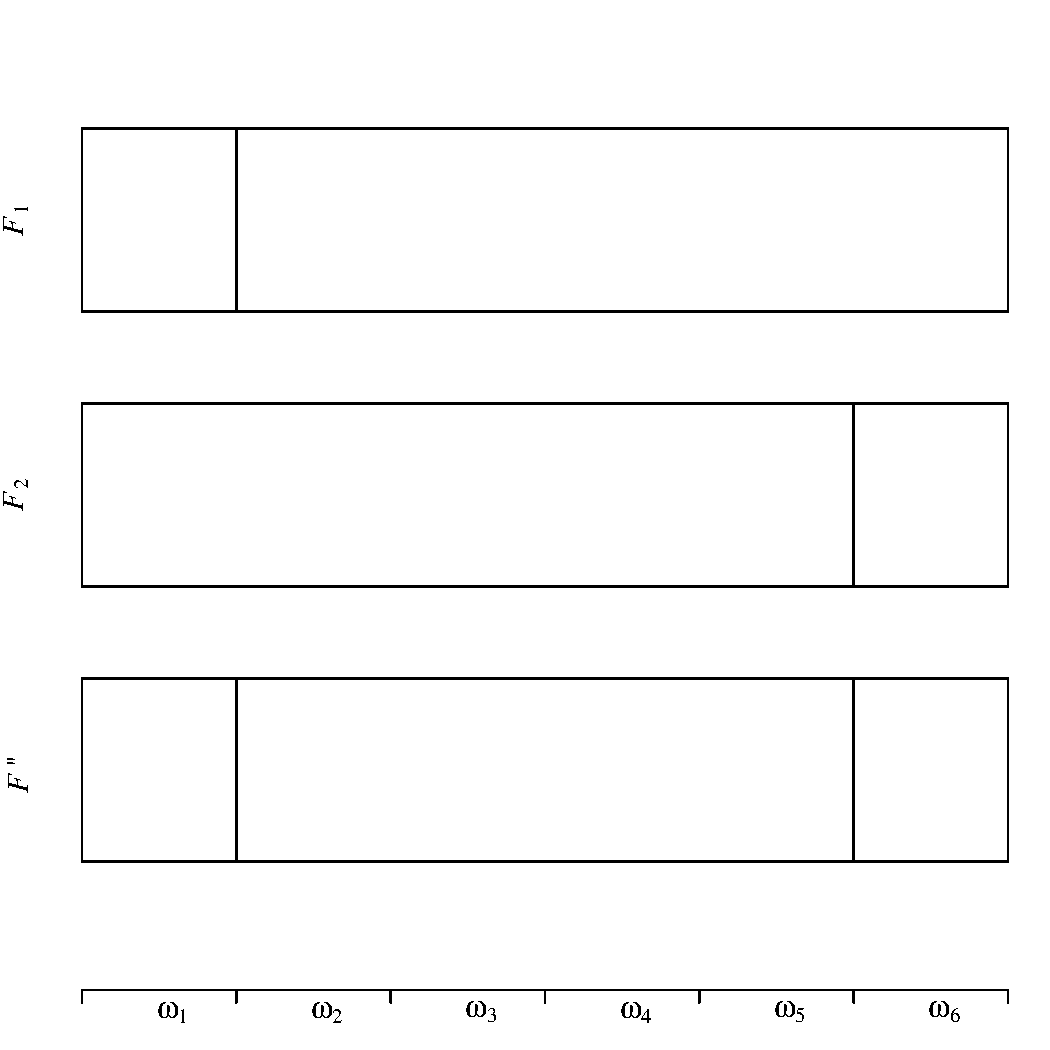
\includegraphics[width = \linewidth]{plots/Finite.pdf} % requires the graphicx package
%   \caption{The information sets $\F_1$ and $\F_2$ in Example \ref{Example1} are generated by the above partitions of $\Omega = \{\omega_1, \dots, \omega_6\}$. The collected information $\F''$ is then generated by the partition induced by considering all interactions of the forecasters' partitions.}
%   \label{ExamplePartitionFinite}
%\end{minipage}
%\hspace{0.7em}
%\begin{minipage}[t]{.48\textwidth}
   \centering
   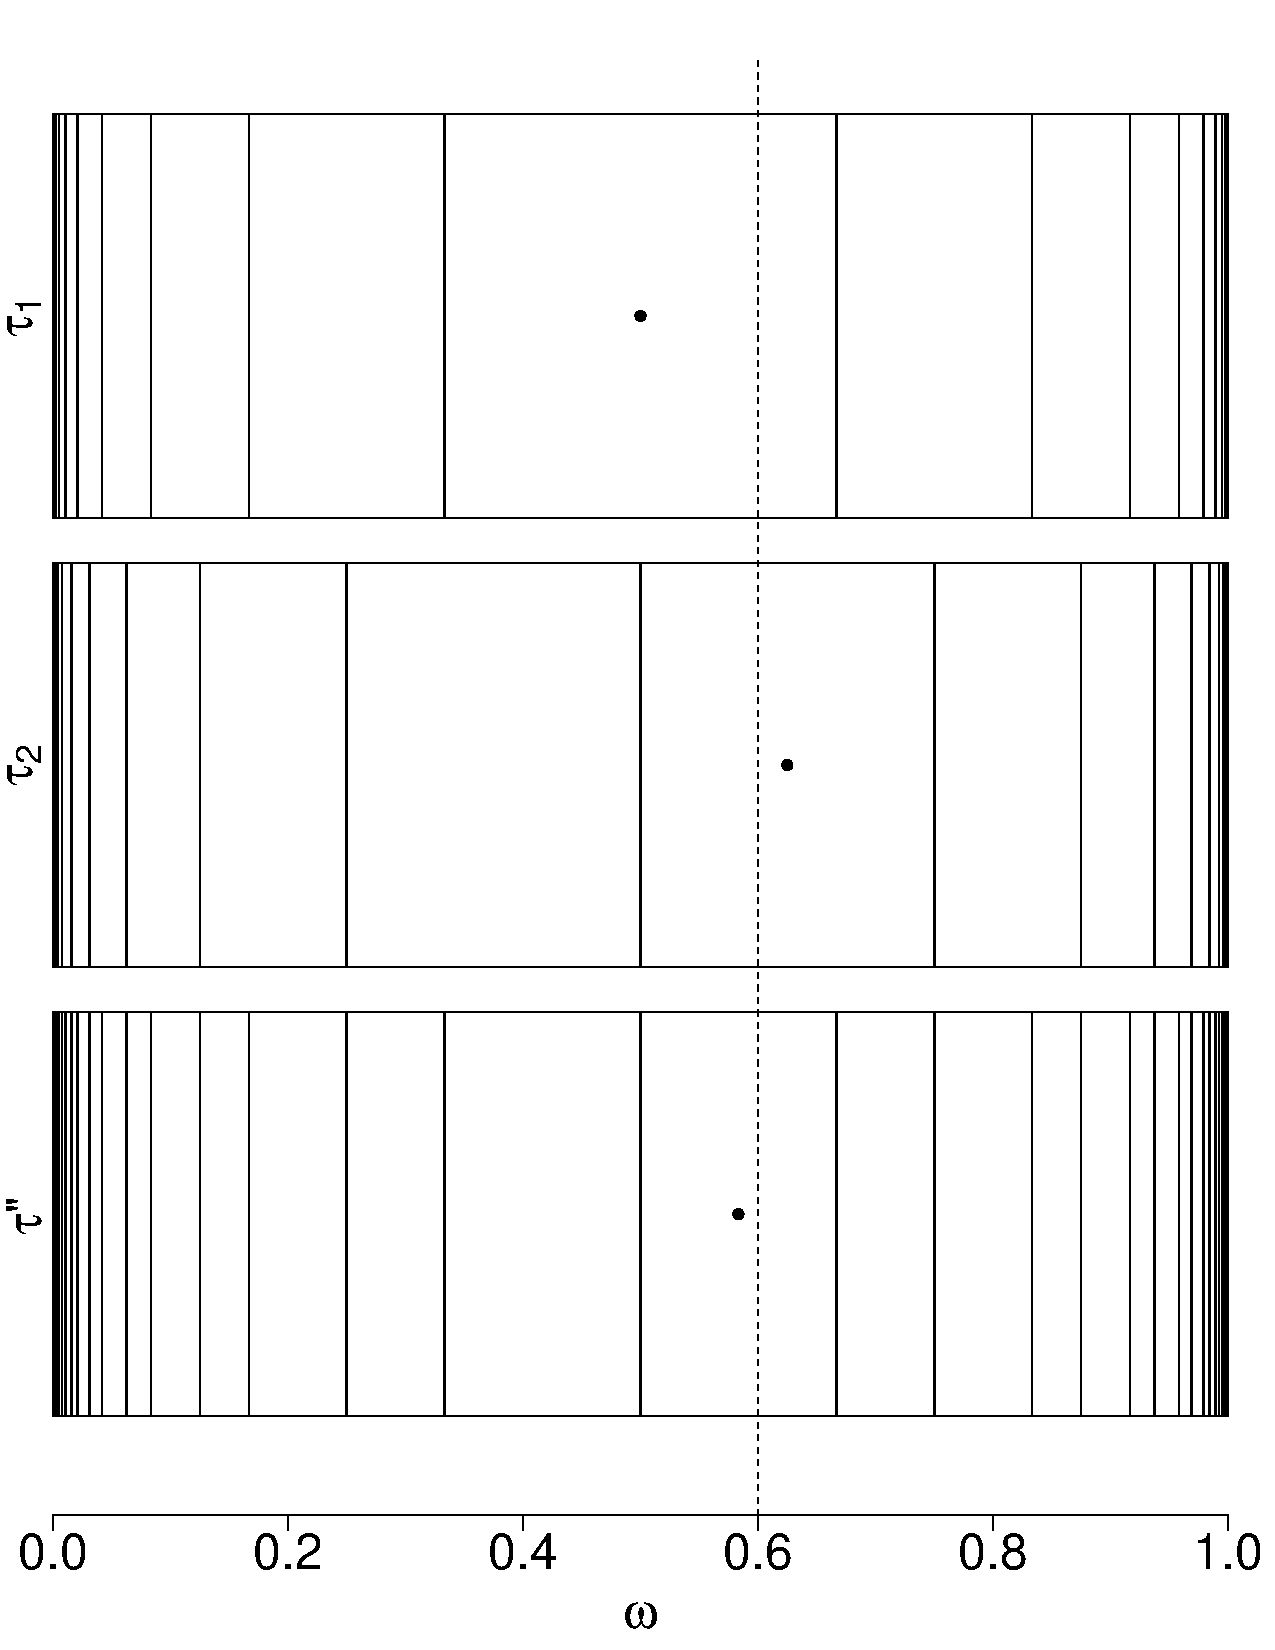
\includegraphics[width = 0.5\linewidth, height = 0.45\linewidth]{plots/Countable.pdf} % requires the graphicx package
   \caption{The partitions $\tau_1$ and $\tau_2$ generate the forecasters' information. Together they form the partition $\tau''$ that generates the forecasters' combined information $\tau''$. Under Lebesgue measure the predictions are the middle points of each interval. For instance, if $\omega = 0.6$ (the dashed line), then predictions are the points on the graph. Observe how $\mathcal{X}''$ is strictly between $X_1$ and $X_2$ under each $\omega \in [0,1]$.}
   \label{ExamplePartition}
%\end{minipage}
\end{figure}


%\begin{figure}[t!]
%   \centering
%   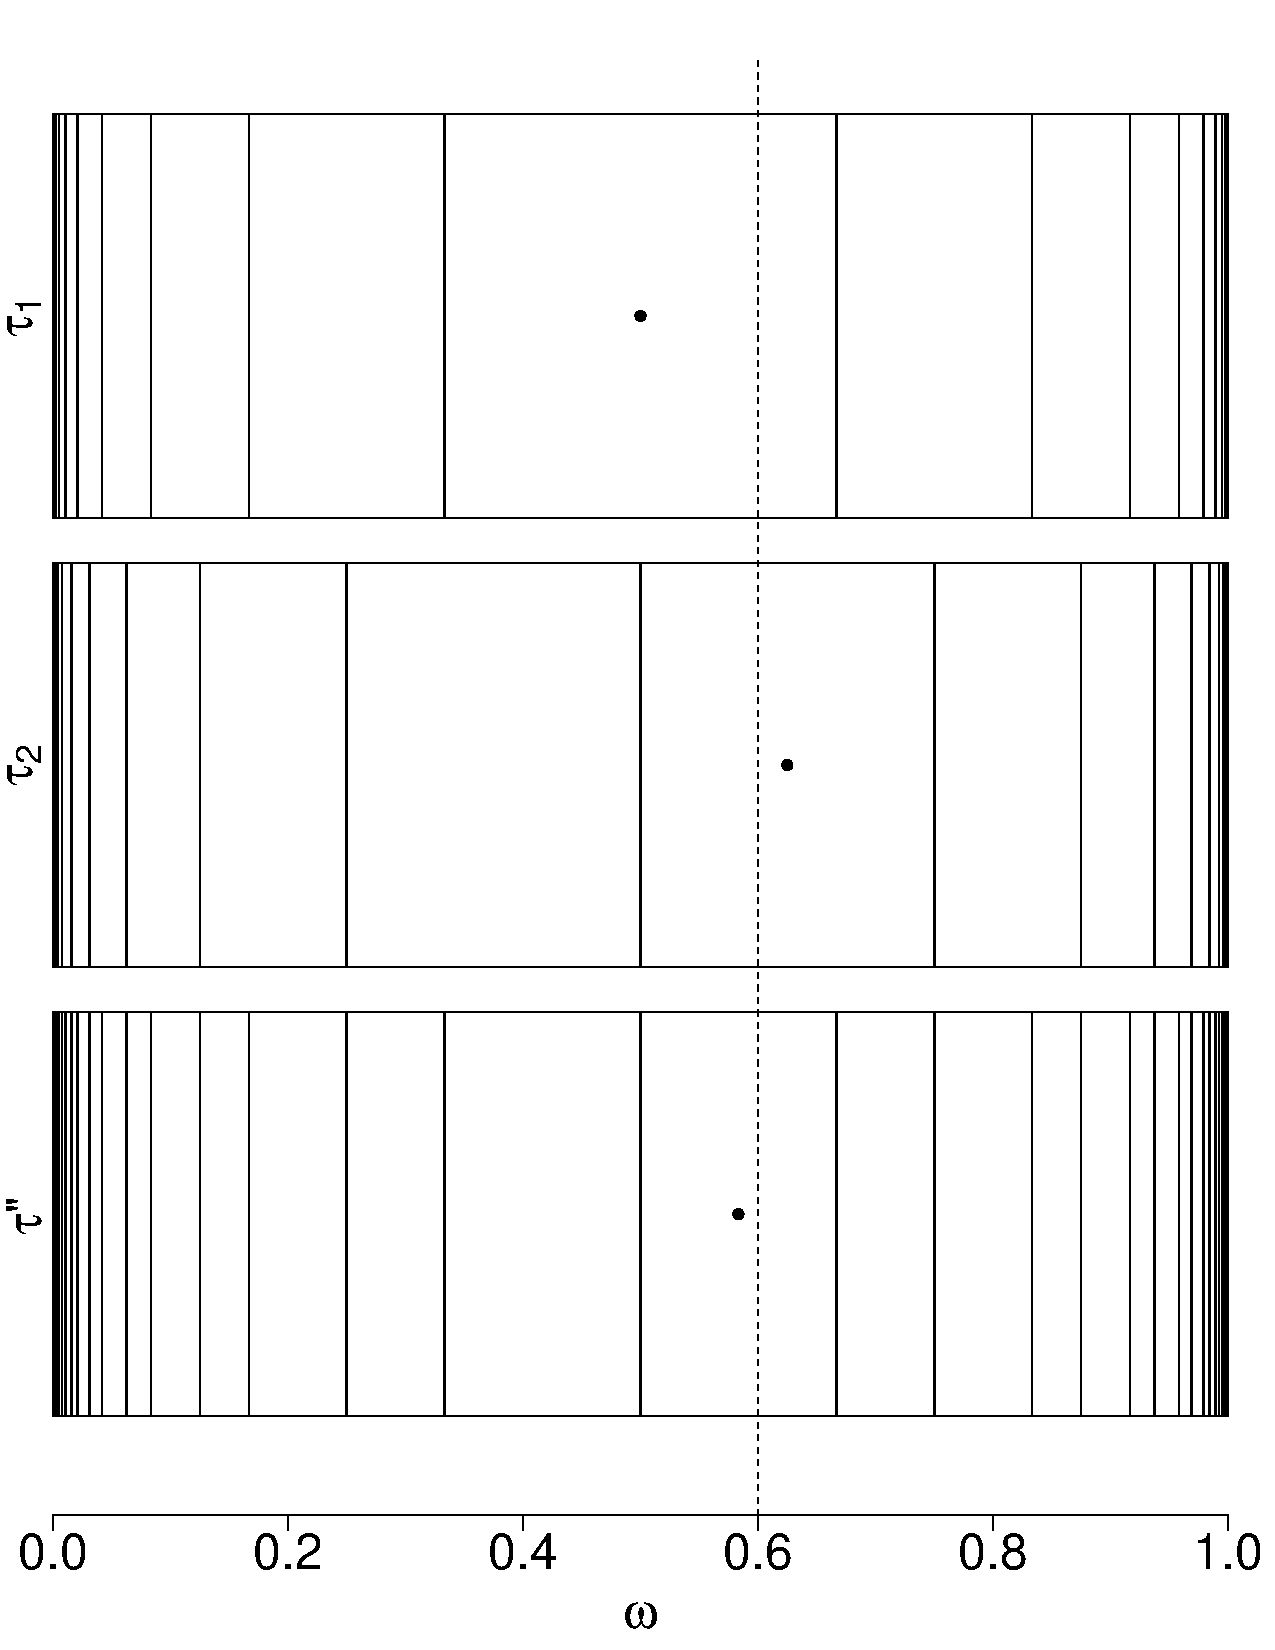
\includegraphics[width = 0.5\linewidth]{plots/Countable.pdf} % requires the graphicx package
%   \caption{The partitions $\tau_1$ and $\tau_2$ generate the forecasters' information. Together they form the partition $\tau''$ that generates the revealed information. Under Lebesgue measure the predictions are the middle points of each interval. Observe how $X''$ is strictly between $X_1$ and $X_2$. }
%   \label{ExamplePartition}
%\end{figure}
%
%\begin{example}
%Consider a probability space $(\Omega, \F, \P)$, where $\Omega = \R$ and $\F$ is the Borel $\sigma$-field. Let the target outcome be $Y(\omega) = \omega$. Consider two forecasters with the following information sets: 
%\begin{align*}
%\F_1 &= \sigma(\dots, [-2 -1), [-1, 0), [0, 1), [1, 2), [2, 3), \dots)\\
%&= \sigma\left(A_j := [j,j+1) : j \in \mathbb{Z}\right)\\
%\F_2 &= \sigma(\dots, [-1.5, -0.5), [-0.5, 0.5), [0.5, 1.5), [1.5, 2.5), [2.5, 3.5), \dots)\\
%&= \sigma\left(B_j := [j-0.5,j+0.5) : j \in \mathbb{Z}\right)\\
%\F'' &= \sigma(\dots, [-1, -0.5), [-0.5, 0), [0, 0.5), [0.5, 1), [1, 1.5), \dots)\\
%&= \sigma\left(C_j := [j/2,j/2+0.5) : j \in \mathbb{Z}\right)
%\end{align*}
%Suppose that $\P(C_j) > 0$ for all $j \in \mathbb{Z}$. Each of these information sets is generated by a countably infinite partition of $\Omega$. This setup is illustrated in Figure . The predictions here are 
%\begin{align*}
%X_1(\omega) = \E(Y|\F_1)(\omega) &= \sum_{i}\frac{\int_{A_i} Y d\P}{\int_{A_i}1 d\P} \one_{A_i} = \sum_{i}\frac{\E( \one_{A_i} Y )}{\P(A_i)} \one_{A_i} \text{ a.s.}\\
%X_2(\omega) = \E(Y|\F_2)(\omega) &= \sum_{j}\frac{\int_{B_j} Y d\P}{\int_{B_j}1 d\P} \one_{B_j} = \sum_{j}\frac{\E( \one_{B_j} Y )}{\P(B_j)} \one_{B_j}\text{ a.s.}\\
%X''(\omega) = \E(Y|\F'')(\omega) &= \sum_{k}\frac{\int_{C_k} Y d\P}{\int_{C_k}1 d\P} \one_{C_k} = \sum_{k}\frac{\E( \one_{C_k} Y )}{\P(C_k)} \one_{C_k}\text{ a.s.}\\
%\end{align*}
%\end{example}
%

\begin{example} \label{uncountable}
Consider $N = 2$ forecasters predicting a proportion based on some private and shared information. Suppose the proportion is uniformly distributed over the unit interval and that the forecasters are better at predicting proportions near zero and one. This can be described with the standard probability space $(\Omega, \F, \P)$, where $\Omega = [0,1]$, $\F$ holds all the Borel subsets $\mathcal{B}([0,1])$, and $\P$ is the Lebesgue measure on $[0,1]$. The target proportion is defined as $Y(\omega) = \omega$ for all $\omega \in \Omega$. 
%In other words, $Y$ is uniform over the unit interval. 
%Consider $N = 2$ forecasters. 

To form the forecasters' information, pick two strictly increasing sequences $\tau_1 = \{a_k : k \in \mathbb{Z}\}$ and $\tau_2 = \{b_k : k \in \mathbb{Z}\}$
%\begin{align*}
%%\tau_1 &= \{\dots, a_{-3}}\} \\
%\tau_1= \{\dots, a_{-2}, a_{-1}, a_0, a_1, a_2, \dots\} && \text{and} &&
%%= \left\{\dots, \frac{1}{12}, \frac{1}{6}, \frac{1}{3}, \frac{2}{3}, \frac{5}{6}, \frac{11}{12}, \dots\right\} = \left\{\frac{1}{2} \pm \left( \frac{1}{6} - \frac{\gamma_k}{3} \right): k \in \mathbb{N}\right\}\\
%%\tau_2 &= \{b_k :  k \in \mathbb{N}, b_k \in [0,1], b_k < b_{k+1}\} 
%\tau_2= \{\dots, b_{-2}, b_{-1}, b_0, b_1, b_2, \dots\}
%% = \left\{\dots, \frac{1}{8}, \frac{1}{4}, \frac{1}{2}, \frac{3}{4}, \frac{7}{8}, \dots\right\} =  \left\{\frac{1}{2}, \frac{1}{2} \pm \frac{\gamma_k}{4} : k \in \mathbb{N}\right\},
%\end{align*}
such that both $a_k$ and $b_k$ converge to $0$ as $k \to -\infty$ and to $1$ as $k \to \infty$.
%$a_{-k} \downarrow 0$, $b_{-k} \downarrow 0$, $a_k \uparrow 1$, and $b_{k} \uparrow 1$ as $k \to \infty$. 
Suppose further that the sequences alternate in magnitude such that $a_{k} < b_{k} < a_{k+1} < b_{k+1}$ for all $k \in \mathbb{Z}$. For instance, one can let
%%based on the following points:
\begin{align}
\tau_1 &= 
%\{\dots, a_{-1}, a_0, a_1, \dots\} = \left\{\dots, \frac{1}{12}, \frac{1}{6}, \frac{1}{3}, \frac{2}{3}, \frac{5}{6}, \frac{11}{12}, \dots\right\} =
 \left\{\frac{1}{2} \pm \left( \frac{1}{6} - \frac{\gamma_k}{3} \right): k \in \mathbb{N}\right\} & \text{ and } && \tau_2 &=
% \{\dots, b_{-1}, b_0, b_1, \dots\} = \left\{\dots, \frac{1}{8}, \frac{1}{4}, \frac{1}{2}, \frac{3}{4}, \frac{7}{8}, \dots\right\} =  
 \left\{\frac{1}{2}, \frac{1}{2} \pm \frac{\gamma_k}{4} : k \in \mathbb{N}\right\}, \label{specificChoice}
\end{align}
%Consider two forecasters with the following information sets: 
%\begin{align*}
%\F_1
%% &= \sigma(\dots, A_{-1}, A_0, A_1, \dots)\\
%%&= \sigma(\dots, [1/12, 1/6), [1/6, 1/3), [1/3, 2/3], (2/3, 5/6], (5/6, 11/12], \dots)\\
%&= \sigma\left(\left[2/3 - \gamma_{k+1}/3, 2/3 - \gamma_{k}/3\right), [1/3, 2/3], \left(2/3 + \gamma_{k}/3, 2/3 + \gamma_{k+1}/3\right] \right)\\
%\F_2 
%%&= \sigma(\dots, [1/16, 1/8), [1/8, 1/4), [1/4, 1/2], (1/2, 3/4], (3/4, 7/8], (7/8, 15/16], \dots)\\
%&= \sigma\left(\left[1/2 - \gamma_{k+1}/4, 1/2 - \gamma_k/4\right), [1/4, 1/2], (1/2, 3/4], \left(1/2 + \gamma_k/4, 1/2 + \gamma_{k+1}/4 \right] \right)
%%\\
%%&= \sigma\left(\left[\frac{1}{6} - \frac{1}{3}\sum_{j=0}^{k+1} \left( \frac{1}{2}\right)^j,\frac{1}{6} - \frac{1}{3}\sum_{j=0}^k \left( \frac{1}{2}\right)^j \right), \left(\frac{2}{3} + \frac{1}{3}\sum_{j=0}^{k} \left( \frac{1}{2}\right)^j,\frac{2}{3} + \frac{1}{3}\sum_{j=0}^{k+1} \left( \frac{1}{2}\right)^j \right]: k \in \mathbb{N}\right)
%\end{align*}
where $\gamma_k = \sum_{j=0}^{k} \left( \frac{1}{2}\right)^j \to 2$ as $k \to \infty$. These sequences are illustrated in Figure \ref{ExamplePartition}. 


Any such sequences $\tau_1$ and $\tau_2$ define two countably infinite partitions of $\Omega$. The atoms of these partitions accumulate only at the extremes, and no atom in one partition is contained within an atom in the other partition.
%Given that $\gamma_k \to 2$ as $k \to \infty$, each collection forms a countably infinite partition of $\Omega$. 
The $j$th forecaster's information set $\F_j$ is then generated from the partition defined by $\tau_j$. This computes all possible disjoint unions of the atoms. The result is an uncountably infinite information set because it has the same cardinality as the power set of a countably infinite set. 
%The information set then has the same cardinality as the power set, which is uncountably infinite. 
 Their combined information $\F''$ is generated by the partition
%\begin{align*}
$\tau'' = \tau_1 \cup \tau_2 = \{\dots, a_{-1}, b_{-1}, a_0, b_0, a_1, b_1, \dots\}$. 
%\end{align*}

The predictions $X_1$, $X_2$, and $\mathcal{X}''$ equal the middle points of those atoms to which the realized $\omega \in \Omega$ belongs. In other words, if $\omega \in [a_j, a_{j+1}] \cap [b_i, b_{i+1}]$, then 
\begin{align}
X_1 &= (a_j+a_{j+1})/2, &
X_2 &= (b_i+b_{i+1})/2, &
\mathcal{X}'' &= \begin{cases}
(b_i+a_{j+1})/2 & \text{ if } a_j < b_i\\
(b_{i+1}+a_{j})/2 & \text{ if } a_j > b_i
\end{cases}. \label{Example2Rev}
\end{align}
Given the way the values of $\tau_1$ and $\tau_2$ alternate, $\mathcal{X}''$ is always strictly between $X_1$ and $X_2$. This shows that $\mathcal{X}_{(\cdot)}$ (and hence $\mathcal{X}_{[\cdot]}$) can be efficient if the forecasters' information sets are allowed to be uncountably large. 

Under the specific sequences (\ref{specificChoice}), the efficient aggregator (\ref{Example2Rev}) becomes
\begin{align*}
\mathcal{X}''
%&= \begin{cases}
%\frac{1}{3}X_1 + \frac{2}{3}X_2 & \text{ if } X_1 < X_2\\
%\frac{2}{3}X_1 + \frac{1}{3}X_2 & \text{ if } X_1 > X_2
%\end{cases}\\
&= \begin{cases}
\frac{2}{3} \min(X_1,X_2) + \frac{1}{3} \max(X_1,X_2) & \text{ if } X_2 < 0.5\\
\frac{1}{3} \min(X_1,X_2) + \frac{2}{3} \max(X_1,X_2) & \text{ if } X_2 > 0.5\\
\end{cases}.
% \label{SpecificX}
\end{align*}
This is an arithmetic mean but the weights depend on the realized values of the predictions. In particular, a weight of $2/3$ is given to the prediction that is closer to the nearest extreme value (at $0.0$ or $1.0$). Compared to the equally weighted arithmetic mean $(X_1+X_2)/2$, the aggregator $\mathcal{X}''$ is further away from the marginal mean $\mu_0 = \E(X_j) = 0.5$ and hence more confident. 
%Thus transforming the equally weighted arithmetic mean would improve its expected performance (recall Section \ref{contractionSection}). 

% $X''(\omega) = (b_i+a_{j+1})/2$ if $a_j < b_i$ and otherwise $X''(\omega) = (b_{i+1}+a_{j})/2$ if $a_j < b_i$ 
% The revealed information is
%\begin{align*}
%\F'' &= \sigma(\dots, [1/12, 1/6), [1/4, 1/3), [1/3, 1/2], (2/3, 5/6], (5/6, 11/12], \dots)\\
%\end{align*}
%CAN YOU CHOOSE THESE SUCH THAT THE AGGREGATE IS THE GEOMETRIC MEAN.
\end{example}


%\marginpar{Explain a bit of the intuition of why the result faiils in infinitely large info set}

%\marginpar{Talk about the limits where it is equal}


%Thus  $\mathcal{X}_{(\cdot)}$ and hence $\mathcal{X}_{[\cdot]}$ can be efficient if $\F_j$ are allowed to be uncountably large. This and the other results of this section are summarized in 
%Table \ref{Results} summarizes the results of this section and points out where an inefficiency result was found (\cmark) and where it cannot be found (\xmark). The most general result about the inefficiency of measures of central tendency would have shown $\mathcal{X}_{[\cdot]}$ to be inefficient under any cardinality of $\F_j$ (the bottom row of the Table \ref{Results}). Given that $\mathcal{X}_{[\cdot]}$, however, can be efficient under both finite and uncountable $\F_j$,  the class of aggregators had to be tightened. This was done minimally by not allowing the aggregate to equal the minimum or maximum prediction when at least two predictions differ. The efficiency of this new aggregator $\mathcal{X}_{(\cdot)}$ was then tested across an exhaustive list of different cardinalities of $\F_j$. The results show that $\mathcal{X}_{(\cdot)}$ is inefficient only if $\F_j$ are finite. This kind of a top-down view of our progression suggests that the inefficiency of aggregators with central tendency most likely cannot be generalized much further, offering our theoretical development a natural stopping point. 
%
%\marginpar{It may be that some mixture of these can lead }
%
%% Requires the booktabs if the memoir class is not being used
%\begin{table}[t]
%   \centering
%   %\topcaption{Table captions are better up top} % requires the topcapt package
%   \begin{tabular}{ccc} % Column formatting, @{} suppresses leading/trailing space
%% &  \multicolumn{2}{c}{Cardinality of $\F_j$} \\
% Aggregator&  Finite $\F_j$ & Uncountable $\F_j$ \\ \hline
%%  && \\
%$\mathcal{X}_{(\cdot)}$  & \cmark& \xmark\\
%$\mathcal{X}_{[\cdot]}$ &\xmark& \xmark\\
%   \end{tabular}
%   \caption{Are the aggregators generally inefficient? \cmark = Yes, \xmark = No.}
%   \label{Results}
%\end{table}

%The specific partitions (\ref{specificChoice}) were chosen because they lead to an information collector (\ref{SpecificX}) that is clearly within Definition \ref{Xsc}. Therefore if $\F_j$, for $j = 1, \dots, N$, are allowed to  be uncountably large, $\mathcal{X}_{(\cdot)}$ can collect information.  

%\marginpar{What is the intuition of why they fail? This may be hard.}


%Of course, it is possible to imagine many different examples where the information collector is a random strict convex combination. been constructed specifically such that it is clearly a reasonable measure of central tendency. Can we think of a real world example where we would give more weight to a maximum forecast?
%The results, however, deserve some discussion. In particular, 
Given that the inefficiency of the means (Theorem \ref{centralTendency}) does not hold under uncountably large information sets, it is natural to ask whether such sets even exist in the real world. 
%Suppose, for instance, that the forecaster first observes a random variable $Z$ and then makes a prediction based on this information. If $Z$ only takes upon a finite number of different values, then the forecasters information set will be finite; that is, $|\sigma(Z)| < \infty$. If, on the other hand, $Z$ takes upon an infinite number of different values, then the information set will be uncountable. 
The answer is ``no'' because information content is finite in the physical world \citep{hibbard2014self}. In fact, according to \cite{lloyd2002computational}, the observable universe has a finite information capacity of at most $10^{120}$ bits. Even if the universe did contain infinite information, forecasters could not process it. Computers have finite memory and represent the world in a discrete form. 
%For instance, consider an algorithm that makes predictions based on a dataset. There are only finitely many values this dataset can realize on the computer's finite and discrete memory. Thus the dataset generates a finite $\sigma$-field. 
%Human forecasters, however, live in a continuous world and base their predictions on their past experience. 
%Is this realized as a infinite variable or as a finite variable? It is certainly an uncountable variable but is it processed as such by the human? 
Similarly, the human cognition is limited in its ability to process information.
% See  brain is a finite physical object, made out of a finite number of different particles. If this is considered the random variable leading to the forecast, it is finite and hence generates a finite information set. 
Therefore, even though a forecaster with infinite information may be a convenient approximation in some theoretical work, it is not a precise description of reality. \cite{casella2002statistical} even argue that in practice $|\Omega| < \infty$ (and hence $|\F_j| < \infty$ for all $j$) because measurements cannot be made with infinite precision. Either way, we conclude that (strict) means can be efficient aggregators of calibrated predictions in theory but not in practice.
%This gives us the following corollary.
%\begin{corollary}[Inefficiency of Measures of Central Tendency] \label{MCTCor}
%For all practical purposes, measures of central tendency are not efficient aggregators of information-driven predictions.
%%do not use the forecasters' information efficiently. 
%\end{corollary}
%This result concludes the theoretical development of this paper. The next section summarizes the results and explains how they relate to other areas of forecasting literature. 
%
%\marginpar{Mention something about the tightness of the results. How it seems like this is it!}
%
%\marginpar{This last example also shows that infinite sigma fields and convex combo cannot be efficient. This covers all bases, of a two by two grid. }

%\marginpar{How does this relate to prediction markets and how they collect information.}

It may be that under some additional restrictions on the predictions and outcome the entire class of means is inefficient. Given, however, that we begun with the most general hypothesis  ``all means are inefficient'' and then justified each necessary specification with a concrete example, we believe that Theorem \ref{centralTendency} is very close, if not equal, to the most general version of the inefficiency of the means.


%\marginpar{It may be that some extra conditions can be added such that the entire mean is inefificent under that condjtion of the predictions and outcoems. However, we believe that this results is very close to the general inefficiency of the means. As general as it will get. What would that mean: it would require us to put more constraints on the prerictiosn and outcomes.}


%Consequently, in practice no measure of central tendency collects information from calibrated predictions.
% While these arguments may seem overly philosophical, they emphasize both the highly theoretical nature of our results in Section and also the general scope of the results in Section . 
%\url{https://arxiv.org/pdf/1411.1373.pdf} 

%\marginpar{Write the final result as a corollary: only collects information if uncountable information sets}

%Another example would consider $\Omega = \R$ with Gaussian measure on it. Then we can have overlapping sets that drifts off to infinity. The aggregate must always be in the middle. 


%Explain why average here does not reduce to a fixed weight average. 

%To appreciate how subtle the difference is: Note that each countably infinite set can be modified such that the difference between the new finite set and the original countably infinite set has only measure $\epsilon > 0$. This can be made vanishing small, and hence small enough to not make a difference in practice. An average can never collect information over the modified sets but it can over the non-modified. Yet, we may not observe the difference between the predictions in a million years. The countably infinite case is only the limiting case of the finite partition theory. 
%
%These $\sigma$-fields are actually uncountable. To see this, let $\{C_k : k =1, \dots\}$ denote the countable partition of $\Omega$. Then each $C \in \F''$ can be written as some union 


%This shows that averaging like techniques only work when people have infinite information. Is this realistic? That is what the next subsection talks about.


%\marginpar{This contradicts the Page hypothesis}


%roughly 100 million neurons and 100 billion synapses linking the neurons together. Every possible setting of these is a realization of a random variable. Given that this is a finite object with only finitely many states, the information generated by this random variable is contained in a finite $\sigma$-field. 




%\subsection{Random Strict Convex Combinations}
%\marginpar{The only assumption here is that we are assuming each sigma-field to be generated by a finite collection}
%%\textbf{Suppose that $X'' = \sum_{j=1}^N w_jX_j$ for some random $w_j \in (0,1)$ such that $\sum_{j=1}^N w_j = 1$}\\
%\textbf{Suppose that $X'' \in (\min\{X_1, \dots, X_N\}, \max\{X_1, \dots, X_N\})$ a.s.}\\
%\\
%Consider probability space $(\Omega, \F, \P)$. Suppose $\E | Y | < \infty$ and that $\F_j = \sigma(A_{ij} : i = 1, 2, \dots)$ are generated by  countable partitions of $\Omega$. The generator of the cumulative information is formed by taking all intersections $\F'' = \sigma(C_1, C_2, \dots)$.
%% It is known that every $\sigma$-field on a countable set $\Omega$ can be generated by a countable partition.  
%%Note that all of these partitions must satisfy the law of total expectation: $\E[Y] = \sum_i^I \E[Y | A_i] \P(A_i)$. This shows the overall budget. 
%% (To justify the use of a partition: \url{http://math.stackexchange.com/questions/1441596/show-the-sigma-algebra-of-a-countable-set-is-generated-by-a-partition})
%%We can merge each $w \in C_{ij}$ into a single $w$ with the combined measured because none of the observables change if one moves from one $w$ to another within the same $C_{ij}$. Therefore we can assume that each $C_{ij}$ holds only one $w$. 
%Observe that $X_j$ remains constant over any set $A_{ij}$. The set $A_{ij}$ can be written as a unique union of some $C_k$'s. More specifically, 
%\begin{align*}
%X_j(A_{ij}) = \frac{\sum_{\omega \in A_{ij}} \P(\omega) Y(\omega)}{\sum_{\omega \in A_{ij}} \P(\omega)} &= \frac{\sum_{k : C_k \cap A_{ij} \neq \emptyset}\sum_{\omega \in C_k} \P(\omega) Y(\omega)}{\sum_{\omega \in A_{ij}} \P(\omega)}\\
% &= \frac{\sum_{k : C_k \cap A_{ij} \neq \emptyset}X''(C_k) \sum_{\omega \in C_k} \P(\omega) }{\sum_{\omega \in A_{ij}} \P(\omega)}\\
% &= \sum_{k : C_k \cap A_{ij} \neq \emptyset}p_{ijk}X''(C_k),
%\end{align*}
%where $p_{ijk} = \sum_{\omega \in C_k} \P(\omega)  / \sum_{\omega \in A_{ij}} \P(\omega)$ such that $\sum_{k : C_k \cap A_{ij} \neq \emptyset}p_{ijk} = 1$. 
%%Given that the weights $w_j \in (0,1)$, $X''$ is always in the interior of the convex hull of the predictions; that is, $X''(\omega) \in (\min\{X_j(\omega)\}, \max\{X_j(\omega)\})$. 
%Note that all predictions remain constant over any set $C_k$. 
%Hence it is sufficient to consider the sets $C_k$ instead of the individual $\omega$'s. Define the index for the minimum prediction over a set $C_k$ as ${j}^* := \argmin_j\{X_j(C_k)\}$ and index for the maximum prediction as $j^{**} := \argmax_j\{X_j(C_k)\}$. Given that $X''$ is always in the interior of the convex hull of the predictions, for all sets $C_k$, we have that
%% Similarly define $q_{jk} = \sum_{w \in C_k} \P(w)  / \sum_{w \in B_j} \P(w)$. 
%% and hence would contradict our assumption.
%%\scriptsize
%\begin{align*}
%X_{j^*}(C_{k}) &< X''(C_{k}) < X_{j^{**}}(C_{k})\\
%\Leftrightarrow \sum_{k' : C_k \cap A_{ij^*} \neq \emptyset, C_{k'} \cap A_{ij^*} \neq \emptyset}p_{ij^*k'}X''(C_{k'}) &<  X''(C_k)  <   \sum_{k' : C_k \cap A_{ij^{**}} \neq \emptyset, C_{k'} \cap A_{ij^{**}} \neq \emptyset}p_{ij^{**}k'}X''(C_{k'})\\
%%\frac{\sum_{w \in  A_1 / C_{11}} \P(w) Y(w) + \sum_{w \in C_{11}} \P(w) Y(w)}{\sum_{w \in A_1} \P(w)} &< \frac{\sum_{w \in C_{11}} \P(w) Y(w)}{\sum_{w \in C_{11}} \P(w)}  < \frac{\sum_{w \in B_1 / C_{11}} \P(w) Y(w) + \sum_{w \in C_{11}} \P(w) Y(w)}{\sum_{w \in B_1} \P(w)}\\
%%\frac{\sum_{w \in  A_1 / C_{11}} \P(w) Y(w) + X''(w_1)  \sum_{w \in C_{11}} \P(w) }{\sum_{w \in A_1} \P(w)} &< X''(w_1)   < \frac{\sum_{w \in B_1 / C_{11}} \P(w) Y(w) + X''(w_1)  \sum_{w \in C_{11}} \P(w) }{\sum_{w \in B_1} \P(w)}\\
%%\frac{\sum_{w \in  A_1 / C_{11}} \P(w) Y(w) +   \sum_{w \in C_{11}} \P(w) X''(w_1) }{\sum_{w \in A_1} \P(w)} &< X''(w_1)   < \frac{\sum_{w \in B_1 / C_{11}} \P(w) Y(w) +   \sum_{w \in C_{11}} \P(w) X''(w_1)}{\sum_{w \in B_1} \P(w) }
%\Leftrightarrow \max L_k &< X''(C_k)  < \min U_k,
%\end{align*}
%where
%\begin{align*}
%L_k := \{X''(C_{k'}) : X''(C_{k'}) < X''(C_{k}), C_k \cap A_{ij^*} \neq \emptyset, C_{k'} \cap A_{ij^*} \neq \emptyset\}\\
% U_k := \{X''(C_{k'}) : X''(C_{k'}) < X''(C_{k}), C_k \cap A_{ij^{**}} \neq \emptyset, C_{k'} \cap A_{ij^{**}} \neq \emptyset\} 
%\end{align*}
%Given that $X''(C_k)$ is included on both sides of the strict inequality, we know that $L_k$ and $U_k$ are non-empty. They can be finite or countable.  
%
%\noindent
%\textbf{Countable partitions:} If this is true, then $X''$ must be bounded from below and above by limit points. That is, there is some (potentially infinite) lower bound $l$ such that $X''(C_k) \downarrow l$ monotonically as $k \to \infty$ for some sets of the partition and similarly for an upper bound $X''(C_k) \uparrow u$ monotonically. Note that for each $X''(C_k)$ there is some $X_j$ that is strictly greater (or lower) than $X''(C_k)$.  
%
%%Note that
%%\begin{align*}
%%X''(C_k) &= \sum_{j=1}^N w_j X_j(C_k)\\
%%&= \sum_{j=1}^N w_j X_j(A_{ij} : A_{ij} \cap C_k \neq \emptyset)\\
%%&= \sum_{j=1}^N  \sum_{k' : C_{k'} \cap A_{ij} \neq \emptyset, C_{k} \cap A_{ij} \neq \emptyset} w_j p_{ijk'}X''(C_{k'})
%%\end{align*}
%%Hence each $X''(C_k)$ is a convex combination of some other $X''(C_k)$'s.  Here each $w_j \in (0,1)$ but each $p_{ijk'} \in [0,1]$. Thus $w_jp_{ijk'} \in [0,1)$. They all sum to one. This suggests that at least two difference $X''(C_k)$'s are used in this composition. 
%
%
%\noindent
%\textbf{Finite partitions:} This is a set of $K$ inequalities. In particular, it gives strict upper and lower bounds for each $X''(C_k)$ in terms of the other $X''(C_k)$; that is, each $X''(C_k)$ is upper and lower bounded by some other $X''(C_k)$. This, however, necessarily leads to a cycle of strict inequalities of the form $X''(C_{(1)}) < X''(C_{(2)}) < \dots < X''(C_{(1)})$. To see this, consider a set of $K$ elements $\{x_1, \dots, x_K\}$ in which for each $x_j$ there is some $x_k$ such that $x_j < x_k$ and $j \neq k$. Thus one can begin with a element, say, $x_1$ and always move to another element that is strictly greater. Unfortunately, however, one can make at most $K-1$ steps before the next strictly increasing element is an element that has already been visited. Thus the current element is both strictly smaller and greater than that element. This is a contradiction. Thus such inequalities cannot hold simultaneously. 
%
%\marginpar{When do you have a generator for the sigma field?}
%\marginpar{This assumes a finite partition? Does this need to be the case?}
%%\marginpar{What about equal sets or border case sets? What do we need for this proof to work? Is it enough to just stay that X'' is always strictly inside the convex hull of the predictions.}
%\marginpar{Should we re-write this with integration?}



%, however, is not possible because it implies, for instance, that there is no minimum $X''(C_k)$. 

%\normalsize
%This tells us that $\min\{X''(C_k) : C_k \cap A_1 \neq \emptyset\} < X''(C_1) < \max\{X''(C_k) : C_k \cap B_1 \neq \emptyset\}$. Now if the sets are contiguous, then (again it does not matter how we label)
%\begin{align*}
%p_{11}X''(C_1) + p_{1K}X''(C_{K}) &< X''(C_1)  <  q_{11}X''(C_1)  + q_{12}X''(C_{2}),
%\end{align*}
%which then gives that $X''(C_K) < X''(C_1) < X''(C_2)$. Now repeat this argument for $C_2$ to get that $X''(C_3) < X''(C_2) < X''(C_1)$ (if $X_1(C_2) < X_2(C_2)$)  or $X''(C_1) < X''(C_2) < X''(C_3)$ (if $X_1(C_2) > X_2(C_2)$). Of course, based on what we know from before, only the second case is possible. Hence we have established that $X''(X_K) < X''(C_1) < X''(C_2) < X''(C_3)$. You repeat this argument until the very last set. This then gives you $X''(C_{K-1}) < X''(C_K)$. A contradiction. 





%\subsection{Random Weighted Averaging: Calibration}
%
%The goal in this section is to analyze the (random) weighted average and in particular show that it does not collect information. To keep things tractable, suppose we are working in $L^2(\Omega, \F, \P)$. This is a Hilbert space with all random variables $X \in \F$ such that $\int_\Omega |X|^2 d\P = \E(|X|^2) < \infty$. The inner product is $\langle X,Y \rangle = \E (XY)$. The norm is $||X||^2 = \int_\Omega X^2 d\P = \E(X^2)$. Recall that a Hilbert space is a Banach space; hence every Cauchy sequence converges to an element in the same space. This is important for taking limits. By making this assumption, we are assuming that the outcome $Y$ has $\E(Y^2) < \infty$. 
%
%The Cauchy-Schwartz inequality says that $|\langle X,Y \rangle| \leq \sqrt{\langle X,X \rangle \langle Y,Y \rangle}$. This shows that $-1 \leq \langle X,Y \rangle  / \sqrt{\langle X,X \rangle \langle Y,Y \rangle} \leq 1$, which means that we can interpret it as the cosine of the angle between $X$ and $Y$. Note that if the random variables are assumed to have mean zero, then  $ \langle X,Y \rangle  / \sqrt{\langle X,X \rangle \langle Y,Y \rangle}  =  \E (XY) / \sqrt{ \E (X^2)  \E (Y^2)} = \Corr(X,Y)$
%
%
%%In this vector space, the length $||X||$ is the standard deviation of $X$. 
%
%Any conditional expectation $X_j = \E(Y|\F_j)$ with $\F_j \subset \F$ is an orthogonal projection of $Y$ onto the space of square-integrable random variables measurable with respect to $\F_j$. Call this space $L^2(\F_j)$. Under a Hilbert space such projections are linear contractions. In other words, if $PY = \E(Y|\F_j)$, then $P(\alpha X + \beta Y) = \alpha PX + \beta PY$ and $||\E(Y|\F_j) || =  ||PY|| = \E[(PY)^2] \leq ||Y|| = \E(Y^2)$. These can be easily verified for the conditional expectation. In terms of properties of the projection,  The projections are self-adjoint: for all $X,Y \in L^2$, we have that $\langle PX, Y \rangle = \langle PX, PY \rangle  = \langle X, PY \rangle $.  The projection is idempotent; that is, $P^2 = P$. That is, projecting twice is the same as projecting once. 
%%\item 
%%The converse is also true: if $P$ is a self-adjoint operator in a Hilbert space and if $P^2 = P$, then the range of $P$ is a subspace of the Hilbert space and $P$ is a projection onto that subspace. Thus, an operator is a projection in a Hilbert space if and only if it is self-adjoint and idempotent. Note, however, that not all projections are conditional expectations. In fact, a projection $P$ on $L^2$ is a conditional expectation if and only if it is positive and it leaves the constant function $1$ invariant.   
%An operator on $L^2$ is a conditional expectation if and only if  
%\begin{enumerate}[i)]
%\item preserves unity: $P(1) = 1$. This suggests that $P$ keeps all the constants. 
%\item positive: $PX \geq 0$ for all $X \geq 0$. 
%\item linear operator: $P(\alpha X + \beta Y) = \alpha P X + \beta P Y$ for all possible $X,Y \in L^2$ and constants $\alpha, \beta$. 
%\item idempotent: $P^2 = P$, which means that multiple applications do not change the value beyond the initial application. 
%\item has $||P|| \leq 1$. 
%\end{enumerate}
%
%
%%\item Given that $P$ is self-adjoint, we have that $||P|| = 1$ where the operator is defined as 
%%\begin{align*}
%%||P|| &= \sup_{||Y||^2 = 1} |\langle PY,Y\rangle|\\
%%&= \sup_{||Y||^2 = 1} |\langle PY,PY\rangle|\\
%%&= \sup_{||Y||^2 = 1} | \E(X_j^2)|\\
%%%&= \sup_{ \E(Y^2) = 1} |\E [\E(Y | \F_j) Y]|\\
%%%&= \sup_{ \E(Y^2) = 1} |\E [X_j Y]|\\
%%%&= \sup_{ \E(Y^2) = 1} |\Cov(X_j,Y) + \mu_0^2|\\
%%\end{align*}
%
%%\item 
%%
%%\end{enumerate}
%
%
%
%The study here focuses on $\sum_{j=1}^n w_j X_j$, where each $X_j = \E(Y|\F_j)$ and $\sum_{j=1}^N w_j = 1$. The weights are assumed to be a function of $\{X_j : j = 1, \dots, N\}$ and hence random. Given that each $X_j$ is a function of $Y$, this means that the random weighted average is only a function of $Y$. This aggregator satisfies the following properties:
%
%\begin{enumerate}[i)]
%\item preserves unity: $\phi(1 | \F_1, \dots, \F_N) = \sum_{j=1}^n w_j \E(1|\F_j) = \sum_{j=1}^n w_j  = 1$
%\item positive: If $Y > 0$, then each $\E(Y | \F_j) > 0$. Given that $w_j \in [0,1]$, we have that
%\begin{align*}
%\phi(Y) &=  \sum_{j=1}^n w_j(Y; \F_1, \dots, \F_N) \E( Y|\F_j) \geq 0
%%&=  \alpha \sum_{j=1}^n w_j(\alpha Y_1 + \beta Y_2; \F_1, \dots, \F_N) \E( Y_1 |\F_j) + \beta \sum_{j=1}^n w_j(\alpha Y_1 + \beta Y_2; \F_1, \dots, \F_N) \E(Y_2|\F_j)\\\\
%\end{align*}
%
%
%\item linear operator: \\
%$\Rightarrow$ Suppose $w_j$ is a constant.  Then,
%\begin{align*}
%\phi(\alpha Y_1 + \beta Y_2) &=  \sum_{j=1}^n w_j \E(\alpha Y_1 + \beta Y_2|\F_j)\\
%&=  \sum_{j=1}^n w_j\left[ \alpha \E(Y_1| \F_j) + \beta \E(Y_2|\F_j) \right]\\
%&=   \alpha \sum_{j=1}^n w_j \E(Y_1| \F_j) + \beta \sum_{j=1}^n w_j \E(Y_2|\F_j) \\
%&= \alpha \phi( Y_1) + \beta \phi(Y_2) 
%%&=  \alpha \sum_{j=1}^n w_j(\alpha Y_1 + \beta Y_2; \F_1, \dots, \F_N) \E( Y_1 |\F_j) + \beta \sum_{j=1}^n w_j(\alpha Y_1 + \beta Y_2; \F_1, \dots, \F_N) \E(Y_2|\F_j)\\\\
%\end{align*}
%$\Leftarrow$ Suppose $\phi$ is a linear operator. Then for all $Y_1, Y_2 \in L^2$ we have that 
%\begin{align*}
%\phi(\alpha Y_1 + \beta Y_2) &=   \alpha \phi( Y_1) + \beta \phi(Y_2) \\
%\sum_{j=1}^n w_j(\alpha Y_1 + \beta Y_2) \E(\alpha Y_1 + \beta Y_2|\F_j) &= \alpha \sum_{j=1}^n w_j(Y_1) \E(Y_1| \F_j) + \beta \sum_{j=1}^n w_j(Y_2) \E(Y_2|\F_j) \\
%\sum_{j=1}^n w_j(\alpha Y_1 + \beta Y_2) \left( \alpha\E( Y_1 |\F_j)  + \beta \E(Y_2 | \F_j)\right)&= \alpha \sum_{j=1}^n w_j(Y_1) \E(Y_1| \F_j) + \beta \sum_{j=1}^n w_j(Y_2) \E(Y_2|\F_j) 
%\end{align*}
%Re-ordering the terms gives
%\begin{align*}
%\sum_{j=1}^n \left[ w_j(\alpha Y_1 + \beta Y_2) - w_j(Y_1) \right] \alpha\E( Y_1 |\F_j) + \sum_{j=1}^n \left[ w_j(\alpha Y_1 + \beta Y_2) - w_j(Y_2)\right] \beta \E(Y_2|\F_j)&= 0
%\end{align*}
%This equation has one solution at $w_j(\alpha Y_1 + \beta Y_2) = w_j(Y_1) = w_j(Y_2)$ for all $j = 1, \dots, N$. This shows that the weight functions are constant: they are the same no matter what $Y \in L^2$ is being predicted. When is this the unique solution? All solutions must work for all choices of $\{ \F_j : j = 1, \dots, N\}$ and $\alpha$. We need a subset on which only constant weights work. Setting $\beta = 0$ gives
%\begin{align*}
%\sum_{j=1}^n \left[ w_j(\alpha Y) - w_j(Y) \right] \alpha\E( Y |\F_j) &= 0\\
%\sum_{j=1}^n \left[ w_j(\alpha Y) - w_j(Y) \right] \E( Y |\F_j) &= 0
%\end{align*}
%This does not prove that the functions are constant. It only shows that they are invariable to the choice of units. For instance, think of a weight function that sets $w_j = X_j / (X_1 + \dots + X_N)$. These are random, sum to one, and also invariable to multiplications by a constant. Therefore this is not enough for us to show that the weight functions are constant. Notice, however, that the above weight function does not pass the addition test. This is quite easy to see. What kind of weights would satisfy this? Setting $\alpha = \beta = 1$ gives us
%\begin{align*}
%\sum_{j=1}^n \left[ w_j( Y_1 +  Y_2) - w_j(Y_1) \right] \E( Y_1 |\F_j) + \sum_{j=1}^n \left[ w_j( Y_1 +  Y_2) - w_j(Y_2)\right]  \E(Y_2|\F_j)&= 0
%\end{align*}
%or alternatively
%\begin{align*}
%\sum_{j=1}^n w_j( Y_1 +  Y_2) \left[ \E( Y_1|\F_j)  +  \E(Y_2|\F_j) \right] &=  \sum_{j=1}^n \left[ w_j(Y_1) \E(Y_1| \F_j) + w_j(Y_2) \E(Y_2|\F_j)  \right]
%\end{align*}
%%Looking at each term gives us 
%%
%%\begin{align*}
%%w_j( Y_1 +  Y_2) \left[ \E( Y_1|\F_j)  +  \E(Y_2|\F_j) \right] &= w_j(Y_1) \E(Y_1| \F_j) + w_j(Y_2) \E(Y_2|\F_j)\\
%%w_j( Y_1 +  Y_2) &= w_j(Y_1) \frac{\E(Y_1| \F_j)}{\left[ \E( Y_1|\F_j)  +  \E(Y_2|\F_j) \right] } + w_j(Y_2) \frac{\E(Y_2|\F_j)}{\left[ \E( Y_1|\F_j)  +  \E(Y_2|\F_j) \right] }\\
%%\end{align*}
%
%
%It is important to note here that this is a general statement about the operator. Hence it must hold for any $N$ and $\alpha, \beta$. For instance, let $Z = \alpha Y+\beta$. Then, we must also have 
%\begin{align*}
%\phi( Z) &= \alpha \phi( Y) +\beta\\
%w(Z)\E(\alpha Y+\beta | \F_1) + (1-w(Z))\E(\alpha Y+\beta| \F_2) &= w(Y)\alpha \E(Y | \F_1) + (1-w(Y))\alpha\E( Y| \F_2) + \beta\\
%w(Z) \left( \E( Y | \F_1) - \E( Y| \F_2) \right) &= w(Y) \left( \E(Y | \F_1) - \E( Y| \F_2) \right)\\
%w(\alpha Y + \beta)  &= w(Y),
%\end{align*}
%which shows that $\w(\cdot)$ is invariant to linear transformations. It is important to think about what the weight function really is. It is really a function of $X_j$ as this is what has been observed. Thus one could write $w(X_1, \dots, X_N)$. This result then shows that $w(X_1, \dots, X_N) = w(\alpha X_1 + \beta, \dots, \alpha X_N + \beta)$. In other words, the weight function is invariable to linear transformation of the predictions. For instance, the median behaves like this. Now, let $Z = Y_1 + Y_2$. Then,
%\begin{align*}
%\phi( Y_1 + Y_2) &= \phi( Y_1) + \phi(Y_2)\\
%w(Z)\E(Z | \F_1) + (1-w(Z))\E(Z| \F_2) &= w(Y_1)\E(Y_1 | \F_1) + (1-w(Y_1))\E(Y_1| \F_2) + w(Y_2)\E(Y_2 | \F_1) + (1-w(Y_2))\E(Y_2| \F_2)
%\end{align*}
%
%%Suppose now that $Y$ is not identically zero. In fact, if $Y = 0$, there is not much forecasting to be done. Differentiating (this places some continuity constraints on $w(\cdot)$) both sides by $\alpha$ gives  $Y \frac{\partial }{\partial \alpha} w(\alpha Y) = 0$. If $Y$ is not identically zero, then $ \frac{\partial }{\partial \alpha} w(\alpha Y) = 0$. Next, differentiate both sides by $Y$ to get $\alpha \frac{\partial }{\partial Y} w(\alpha Y) = \frac{\partial }{\partial Y} w(Y)$
%
%
%%\begin{align*}
%%\phi( Y_1 + Y_2) &= \phi( Y_1) + \phi( Y_2)\\
%%%& w\E(\alpha Y_1 + \beta Y_2 | \F_1) + (1-w)\E(\alpha Y_1 + \beta Y_2 | \F_2) \\
%%% &= \alpha[w\E(Y_1 | \F_1) + (1-w)\E(Y_1 | \F_2)]+ \beta[w\E(Y_2 | \F_1) + (1-w)\E(Y_2 | \F_2)]\\
%%%& w\E(\alpha Y_1 + \beta Y_2 | \F_1) + \E(\alpha Y_1 + \beta Y_2 | \F_2) - w\E(\alpha Y_1 + \beta Y_2 | \F_2)\\
%%%  &= \alpha w\E(Y_1 | \F_1) + \alpha\E(Y_1 | \F_2) - \alpha w \E(Y_1 | \F_2)+ \beta w\E(Y_2 | \F_1) + \beta\E(Y_2 | \F_2)] - \beta w \E(Y_2 | \F_2)]\\
%%%& w\E(\alpha Y_1 + \beta Y_2 | \F_1) - w\E(\alpha Y_1 + \beta Y_2 | \F_2)  -  \alpha w\E(Y_1 | \F_1) + \alpha w \E(Y_1 | \F_2) - \beta w\E(Y_2 | \F_1) + \beta w \E(Y_2 | \F_2)]\\
%%% &= \alpha\E(Y_1 | \F_2) + \beta\E(Y_2 | \F_2)] - \E(\alpha Y_1 + \beta Y_2 | \F_2)\\
%%%& w\left( \E(\alpha Y_1 + \beta Y_2 | \F_1) - \E(\alpha Y_1 + \beta Y_2 | \F_2)  -  \alpha \E(Y_1 | \F_1) + \alpha \E(Y_1 | \F_2) - \beta \E(Y_2 | \F_1) + \beta  \E(Y_2 | \F_2)] \right)\\
%%% &= \alpha\E(Y_1 | \F_2) + \beta\E(Y_2 | \F_2)] - \E(\alpha Y_1 + \beta Y_2 | \F_2)\\
%%\end{align*}
%%which gives
%%\begin{align*}
%%w &= \frac{\alpha\E(Y_1 | \F_2) + \beta\E(Y_2 | \F_2) - \E(\alpha Y_1 + \beta Y_2 | \F_2)}{\left( \E(\alpha Y_1 + \beta Y_2 | \F_1) - \E(\alpha Y_1 + \beta Y_2 | \F_2)  -  \alpha \E(Y_1 | \F_1) + \alpha \E(Y_1 | \F_2) - \beta \E(Y_2 | \F_1) + \beta  \E(Y_2 | \F_2)] \right)}
%%\end{align*}
%%We also have the sum constraints. THIS MAY BE COMPLICATED TO SHOW.
%
%\item Idempotent: This applies the procedure twice recursively. In words, the average prediction should be the same as the average of the forecasters' predictions about the consensus. This requires the forecasters to make predictions about each others predictions: that is, compute $\E[\E[Y| \F_i] | \F_j]$. Of course, if one $\sigma$-field is subset of the other, this can be reduced by the "smallest $\sigma$-field wins"-theorem. Typically, however, these $\sigma$-fields are partially overlapping. 
%
%\end{enumerate}
%
%
%Note that each projection $P$ on  $X, Y \in L^2$ we have that $\langle PX, Y \rangle = \langle X, PY \rangle$; that is, they are self-adjoint. The goal now is to show that this is not true for the weighted average. 
%
%\begin{align*}
%\E \left[ X \sum_{j=1}^n w_j(Y) \E(Y|\F_j) \right] &= \E \left[ Y \sum_{j=1}^n w_j(X) \E(X|\F_j) \right] \\
%\E \left[ X \sum_{j=1}^n w_j(Y) \E(Y|\F_j) \right] &= \E \left[ Y\right] \E[X]\\
%\E \left[ \sum_{j=1}^n w_j(Y) \E(Y|\F_j) \right] &= \E \left[ Y\right]\\
%\end{align*}
%The same applies for any constant $Y$. 
%
%
%\subsection{Random Weighted Averaging: Variance Bound}
%
%In this section we are analyzing the variance of $\phi(Y) = \sum_{j=1}^n w_j X_j$. In particular, the goal is to show that this variance is upper bounded by $\delta_{max} = \Var(X_{max})$. To begin, suppose $\phi$ is calibrated. If it is not, then it is not consistent with some information set and we are done. Recall that calibration implies marginal consistent. Hence $\E\phi = \mu_0$. Then,
%\begin{align*}
%\Var\left(\sum_j w_j X_j\right) &= \E\left[ \left(\sum_j w_j X_j\right)^2\right] -\mu_0^2
%\end{align*}
%Given that $\Var(X_{max}) = \E(X_{max}^2) - \mu_0^2$, it suffices to show that 
%\begin{align*}
%\E\left[ \left(\sum_j w_j X_j\right)^2\right] \leq \E(X_{max}^2)
%\end{align*}
%By Jensen's inequality, for any $\omega \in \Omega$, we have that 
%\begin{align*}
% \sum_j w_j X_j^2 -  \left(\sum_j w_j X_j\right)^2 &= \frac{1}{2}\sum_{ij} w_i w_j (X_i - X_j)^2 \\
% \left(\sum_j w_j X_j\right)^2 &=  \sum_j w_j X_j^2 - \frac{1}{2}\sum_{ij} w_i w_j (X_i - X_j)^2 \\
% \left(\sum_j w_j X_j\right)^2 &\leq  \sum_j w_j X_j^2
%\end{align*}
%Taking expectations gives us
%\begin{align*}
% \E \left(\sum_j w_j X_j\right)^2 &=  \sum_j \E (w_j X_j^2) - \frac{1}{2}\sum_{ij} \E[w_i w_j (X_i - X_j)^2]\\
% &=  \sum_j \E (w_j) \E(X_j^2) + \Cov(w_j, X_j^2) - \frac{1}{2}\sum_{ij} \E[w_i w_j (X_i - X_j)^2]\\
% &\leq \sum_j \E (w_j) \E(X_{max}^2) + \sum_j\Cov(w_j, X_j^2) - \frac{1}{2}\sum_{ij} \E[w_i w_j (X_i - X_j)^2]\\
% &=  \E(X_{max}^2) + \sum_j\Cov(w_j, X_j^2) - \frac{1}{2}\sum_{ij} \E[w_{i}w_j (X_i - X_j)^2]
%% &=  \E(X_{max}^2) + \sum_j\Cov(w_j, X_j^2) - \sum_{i<j} \E[w_{ij} (X_i - X_j)^2],
%\end{align*}
%%where $w_{ij} = w_i w_j \leq \min\{w_i, w_j\}$.  
%%This inequality is sharp, with the equality happening when $X_i = X_j$ for all $i \neq j$. Note also that it is trivially true for constant $w_j$ or if $w_j$ is uncorrelated with $X_j$ because in both cases all $\Cov(w_j, X_j^2) = 0$. 
%Therefore it remains to be shown that 
%\begin{align*}
%\sum_j\Cov(w_j, X_j^2) &\leq \frac{1}{2}\sum_{ij} \E[w_{i}w_j (X_i - X_j)^2] \\
%%\sum_j \E[w_j X_j^2] - \sum_j \E[w_j]\E[X_j^2] &\leq \frac{1}{2}\sum_{ij} \E[w_{i}w_j (X_i - X_j)^2] \\
%\E[ \sum_{ij}w_iw_j X_j^2] - \sum_j \E[w_j]\E[X_j^2] &\leq \frac{1}{2}\sum_{ij} \E[w_{i}w_j (X_i - X_j)^2] \\
%\E[ \sum_{ij}w_iw_j X_j^2] - \sum_j \E[w_j]\E[X_j^2] &\leq \frac{1}{2}\left( \sum_{ij} \E[w_{i}w_j X_i^2 - 2w_{i}w_j X_iX_j + w_{i}w_jX_j^2]  \right) \\
%\E[ \sum_{ij}w_iw_j X_j^2] - \sum_j \E[w_j]\E[X_j^2] &\leq \left( \sum_{ij} \E[w_{i}w_j X_i^2 - w_{i}w_j X_iX_j]  \right) \\
% - \sum_j \E[w_j]\E[X_j^2] &\leq - \sum_{ij} \E[w_{i}w_j X_iX_j]   \\
%\E\left[ (\sum_j w_j X_j)^2 \right] = \sum_{ij} \E[w_{i}w_j X_iX_j]   &\leq   \sum_j \E[w_j]\E[X_j^2] = \sum_{ij} \E[w_iw_j]\E[X_j^2]\\
%\end{align*}
%%
%%\begin{align*}
%% \sum_j\Cov(w_j, X_j^2)  &\leq 0\\
%% \sum_j \E[w_jX_j^2] - \E[w_j]\E[X_j^2]  &\leq 0\\
%% \sum_j \E[w_jX_j^2] - \E[w_j](\delta_j + \mu_0^2)  &\leq 0\\
%% \sum_j \E[w_jX_j^2] - \sum_j\E[w_j]\delta_j - \sum_j\E[w_j]\mu_0^2  &\leq 0\\
%% \sum_j \E[w_jX_j^2] - \sum_j\E[w_j]\delta_j  &\leq \mu_0^2\\
%% \sum_j^{N-1} \E[w_jX_j^2] + \E[(1-\sum_j^{N-1}w_j)X_N^2] - \sum_j^{N-1}\E[w_j]\delta_j - (1-\sum_{j}^{N-1}\E[w_j])\delta_N  &\leq \mu_0^2\\
%% \sum_j^{N-1} \E[w_jX_j^2] + \E[X_N^2]-\sum_j^{N-1}\E[w_jX_N^2] - \sum_j^{N-1}\E[w_j]\delta_j - \delta_N+\sum_{j}^{N-1}\E[w_j]\delta_N  &\leq \mu_0^2\\
%% \sum_j^{N-1} \E[w_j(X_j^2-X_N^2)] - \sum_j^{N-1}\E[w_j](\delta_j-\delta_N)   &\leq 0
%%%\\
%%%  \sum_j\Corr(w_j, X_j^2) \Sd(w_j)\Sd(X_j^2) &\leq 0\\
%%% \Leftrightarrow  \sum_j\Cor(w_j, X_j^2) &\leq 0\\
%%\end{align*}
%%The choice of the base group was entirely arbitrary. Suppose then that $X_N = X_{max}$. 
%%\begin{align*}
%% \sum_j^{N-1} \E[w_j(X_{max}^2-X_j^2)]   &\geq \sum_j^{N-1}\E[w_j](\delta_{max}-\delta_j) 
%%\end{align*}
%This show that our inequality holds if the variance of (or simply the quadratic expectation) of our aggregator is less than the expected weighted average of the individual variances. That is, it is true if $\Var(\sum_j w_j X_j) \leq \sum_j \E(w_j) \Var(X_j)$. This all is obviously true when $\sum_{ij} \Cov(w_iw_j, X_iX_j) \leq 0$. Calibration gives us some useful equalities:
%\begin{align*}
%\E[(Y+X_j)^2] = ||Y+X_j||^2 &= ||Y||^2 + 3||X_j||^2 = \E[Y^2] + 3\E[X_j^2]\\
%\E[(Y-X_j)^2] = ||Y-X_j||^2 &= ||Y||^2 - ||X_j||^2  = \E[Y^2] - \E[X_j^2]\\
%\langle X_j, Y \rangle &= \E[X_jY] = \E[X_j^2] = \langle X_j, X_j \rangle\\
%\\
%\\
%\E[(Y+\sum_j w_j X_j)^2] &= \E[Y^2] + 3\sum_{ij} \E[w_iw_j X_jX_i]\\
%\E[(Y-\sum_j w_j X_j)^2] &= \E[Y^2] - \sum_{ij} \E[w_iw_j X_jX_i]\\
% \sum_{ij} \E[w_iw_j X_jX_i] &=  \sum_{j} \E[Y w_j X_j]
%\end{align*}
%These will help us to assume calibration in the computation. Once plugged in, the inequality should hold always. 
%\begin{align*}
%\E\left[ (\sum_j w_j X_j)^2 \right] = \sum_{ij} \E[w_{i}w_j X_iX_j]   &\leq   \sum_j \E[w_j]\E[X_j^2]\\
%\end{align*}
%
%
%\begin{align*}
%\sum_j \Cov(w_j, X_j) &= 0\\
%\\
%\sum_{ij} w_{i}w_j X_iX_j &= \sum_{ij} (w_{i}X_i)(w_j X_j)\\
%&\leq \sqrt{\sum_{ij} (w_{i}X_i)^2} \sqrt{\sum_{ij} (w_j X_j)^2}\\
%&= \sqrt{N\sum_{i} (w_{i}X_i)^2} \sqrt{N \sum_{j} (w_j X_j)^2}\\
%&= N \sum_{j} (w_j X_j)^2\\
%&= \sum_{ij} (w_j X_j)^2\\
%\end{align*}
%
%
%
%We know here that $w_j \in [0,1]$, $\sum_j w_j = 1$, and that each $X_j^2 \geq 0$. We know that these aggregators are not calibrated. Hence it may be a bit odd to assume that. However, it should be the case that $\E(\sum_j w_j X_j) = \mu_0$. This holds if and only if $\sum_j \Cov(w_j, X_j) = 0$. This is essentially satisfied by the maximum counter example. Something else is needed. In short, this is not a measure of centrality. Then what is? How can we characterize this?   A measure of Central Tendency is a typical value around which other figures congregate. A more general definition is as follows: a measure of central tendency $X$ takes on any function of a list $g(X_1, \dots, X_N)$ that is symmetric under any permutation of the list and equates it to the same function with the value of the average replacing each member of the list $g(X_1, \dots, X_N) = g(X, \dots, X)$ (see page 48 in Statistical Techniques for Project Control). This, however, hardly makes sense. For instance, consider $\argmax_{X_j} (X_j - \mu_0)^2$. This clearly is invariable under permutation and returns a constant when given one. Hence it should be an average. It is, however, not reasonable to consider this as a measure of central tendency. It seems that the most reasonable definition is a value that minimizes the sum of distances to all the data points. 
%
%One may also ask: what kind of a function $w(X_j)$ is? Does it increase or decrease in $X_j$? This can then be combined with Chebyshev's to prove results. 
%
%
%
%
%\subsection{Geometric Interpretation of Information Collection}
%


%
%
%\section{EXTREMIZING REAL-VALUED predictions} \label{extremization}
%This section focuses on extremizing the simple weighted average $\bar{X}$ as this is the most common and often the first approach that many practitioners take when aggregating predictions. 
%
%\begin{theorem}\label{middle}
%In expectation $\bar{X}$ is between $\mu_0$ and $X''$. 
%\end{theorem}
%\begin{proof}
%Define $T = (X'' - \bar{X})(\bar{X} - \mu_0)$ and note that $T \geq 0$ if and only if $\bar{X}$ is between $\mu_0$ and $X''$. To see this consider all six possible cases:
%\begin{align*}
%& \text{If $X'' > \mu_0$, then} && &&\\
%& \bar{X} \in (-\infty, \mu_0) & &\bar{X} \in (\mu_0, X'')  & &\bar{X} \in (X'', \infty) \\
%& (+,-) && (+,+) && (-,+)\\
%& \text{If $X'' < \mu_0$, then} && &&\\
%& \bar{X} \in (-\infty, X'') & &\bar{X} \in (X'', \mu_0)  & &\bar{X} \in (\mu_0, \infty) \\
%& (+,-) && (-,-) && (-,+)
%\end{align*}
%Therefore it suffices to show that $\E(T) \geq 0$. This can be shown as follows:
%\begin{align*}
%\E(T) &= \E[(X'' - \bar{X})(\bar{X} - \mu_0)]\\
% &= \E[X''\bar{X} - \mu_0 X'' - \bar{X}^2 + \mu_0 \bar{X}]\\
% &= \E[X''\bar{X} - \bar{X}^2] & &\text{as } \E(X'') = \E(\bar{X}) = \mu_0\\
% &= \frac{1}{N} \sum_j \E\left[X''X_j\right] - \frac{1}{N^2} \E\left[\left( \sum_j X_j\right)^2\right]\\
% &= \frac{1}{N} \sum_j (\delta_j + \mu_0^2)- \frac{1}{N^2} \left[ \sum_j \E(X_j^2) + \sum_{i \neq j} \E(X_iX_j)\right]\\
% &= \frac{1}{N} \sum_j (\delta_j + \mu_0^2)- \frac{1}{N^2} \left[ \sum_j (\delta_j + \mu_0^2) + \sum_{i \neq j} (\rho_{ij} + \mu_0^2)\right]\\
% &= \frac{1}{N} \sum_j \delta_j- \frac{1}{N^2} \left( \sum_j \delta_j + \sum_{i \neq j} \rho_{ij}\right)
%\end{align*}
%Given that $\bSigma \succeq 0$, the off-diagonal $\rho_{ij} \leq (\delta_i + \delta_j)/2$. Plugging this in gives:
%\begin{align*}
%\E(T)  &\geq \frac{1}{N} \sum_j \delta_j- \frac{1}{N^2} \left( \sum_j \delta_j + \sum_{i \neq j} \frac{\delta_i + \delta_j}{2}\right)\\
%&=  \frac{1}{N} \sum_j \delta_j- \frac{1}{N^2} \left( \sum_j \delta_j + \frac{1}{2} \sum_{j} 2(N-1)\delta_j \right)\\
%&=  \frac{1}{N} \sum_j \delta_j- \frac{1}{N^2} N \sum_j \delta_j \\
%&= 0
%\end{align*}
%\end{proof}
%This suggest that the performance of $\bar{X}$ can be improved by extremizing, that is, by moving it away from $\mu_0$ and closer to $X''$. The main challenge, however, is to determine how much? In this section the amount of linear extremization is chosen by minimizing the quadratic loss, that is, find $\alpha$ such that 
%\begin{align}
%\frac{\partial}{\partial \alpha} \E (X'' - (\mu_0 + \alpha(\bar{X} - \mu_0))^2) &= 0 \label{Alpha}
%\end{align}
%
%\begin{theorem}\label{alphaThm}
%Equation (\ref{Alpha}) is solved by
%\begin{align}
%\alpha &= 
%\end{align}
%\end{theorem}
%\begin{proof}
%Exchanging the order of integration and differentiation gives
%\begin{align*}
%\frac{\partial}{\partial \alpha} \E (X'' - (\mu_0 + \alpha(\bar{X} - \mu_0))^2) &= 0\\
% \E(X'' - \mu_0 - \alpha(\bar{X} - \mu_0)) (\bar{X}-\mu_0) &= 0
%\end{align*}
%\end{proof}
%




%
%\section{REAL-WORLD IMPLICATIONS}\label{realworld}
%
%\subsection{Aggregation of Suboptimal predictions} \label{Noisy predictions}
%
%This would require an understanding of the source of noise. This likely to vary widely from application to another. 
%%Hence it is hard to make a general analysis 
%
%Discuss here the aggregation of suboptimal predictions. The results follow as long as the calibration function is invertible. This has often been the case: typically people use a sigmoidal function or even the more flexible isotonic regression (what was the motivation for this). This then means that no information is lost in recalibartion. Then $X''$ is the same in both cases; that is, it does not matter whether you apply the aggregator to the original or the calibrated predictions. Then any fixed function (that collects information) must be exactly the same whether it is applied to the calibrated or original prediction. If it is not collecting information under the calibrated, it is not doing so either under the origin predictions. Write this out as a general corollary here for all the classes of aggregators we did. 
%
%Ok, it is very unlikely that any of these functions will collect information if they don't do so when the predictions are calibrated. However, here is what we know. If the calibration function invertible etc... 
%
%Of course, machine predictions are often quite calibrated to begin with. But even there similar calibration functions have been found successful. 

%\section{UNCALIBRATED predictions} \label{nonExperts}


%\subsection{Partial Information Aggregators}
%
%If means are inefficient, a natural question to ask is whether an efficient aggregator even exists in practice. Fortunately, the answer is ``yes.''  In fact, there are at least two different ways to construct such aggregators.
%% if $\boldsymbol{X} = (X_1, \dots, X_N)$ and $\boldsymbol{\beta}$ is some vector of unknown parameters,
%
%The first approach assumes a functional form for $\mathcal{X}''$. For instance, if the predictions are calibrated and $\mathcal{X}''$ is a linear function of the predictions, then by minimizing the expected quadratic loss it is possible to show that $\mathcal{X}'' = \mu_0 + \diag(\bSigma)'\bSigma^{-1}(\boldsymbol{X}-\mu_0 \one_N)$, where $\boldsymbol{X} = (X_1, \dots, X_N)$ and $\bSigma := \Cov(\X,\X)$ satisfies $\delta_0 -  \diag(\bSigma)'\bSigma^{-1}\diag(\bSigma) \geq 0$. See \cite{satopaamodeling} for more details, including a non-parametric estimation procedure for $\bSigma$.
%% who propose an algorithm for estimating $\bSigma$  under this constraint. 
%%Overall, this approach does not make direct assumptions about the probability measure $\P$ but it does assume a particular form for the aggregator. 
%
%%\marginpar{Explain a bit more: use then nonparameteric versions of covariance and variance.}
%%\marginpar{Assuming calibration provides enough strength to link $Y$ and $X_j$}
%%
%%\marginpar{Explain that we have work in progress looking for a closed form solution but more work is needed.}
%
%%
%%\marginpar{write this in terms of the wiki page}
%%
%%\marginpar{This may or may not require estimating some parameters. Use nonparametric approaches etc.}
%
%The second approach assumes a parametric form for the model distribution $\P$. 
%% recommend a \textit{top-down}-approach that views aggregation as data analysis. The first step is to link the predictions and outcomes under a single model. 
% The efficient aggregator $\mathcal{X}''$ is then found  by either analytically  or  numerically estimating $\mathcal{X}''$ under the chosen model.
%%Under this model, the efficient aggregator $\mathcal{X}''$ is then be derived analytically or approximated numerically 
%%(e.g., \citealt{clemen1986objective}). 
%%This aggregator is efficient and collects information under the chosen model. 
%%The general message in this paper is that measures of central tendency cannot be constructed in this manner. Thus they do not stem from any model of the predictions and outcomes. 
%Of course, choosing a probability model for the predictions and outcomes requires a certain amount of field expertise. If such expertise is not available, one can work with 
%%efficient aggregation can be performed under 
%a generic model such as the \textit{Gaussian partial information model} \citep{satopaamodeling2}. This is a general model that can be used in a wide range of forecasting applications. For instance, it has been applied to forecasters making  predictions of multiple related events \citep{satopaamodeling2} and also to only two forecasters, each making a single probability prediction \citep{ernst2016bayesian}. 
%
%\marginpar{Maybe remove this and add it as a short discussion in the end. This section should be dedicate to the noisy predictions. Prove theorem of adding the noise.}


\section{AGGREGATING NOISY PREDICTIONS} \label{noisy} 
%\marginpar{Explain here the rule based approach vs model based approach}
%\subsection{Models of Noisy Predictions} \label{altModels} 
%%There are several ways to derive new aggregators \citep{hora2013median}. For instance, one can describe desirable properties and then derive aggregators that satisfy those properties \citep{genest1986combining}. 
%%%Unfortunately, if different aggregators satisfy the same properties, it is not clear under what conditions each aggregator is preferred. 
%%An alternative approach is to find an optimal aggregator under some statistical model that then serves as a direct description of the conditions under which the aggregator performs well. 
%%%\cite{dawid1995coherent} call such aggregators coherent. 
%
%%Our results so far depend on the predictions being calibrated.
%%% As explained in Section \ref{outcomes}, this can be a reasonable assumption in some contexts. 
%%Often, however, aggregators are applied directly to non-calibrated predictions. This section examines aggregation efficiency in such contexts by adding noise to each forecaster's ideal prediction. 
%
%
%%Measure of central tendency is often defined as the single most representative value of a distribution. If the observations are different predictions, this value can be considered as the 
%
%The use of a MCT can be explained with the \textit{measurement error framework} (see, e.g., \citealt{hong2009interpreted, lobo2010human, parunak2013characterizing}). This assumes the forecasters to make erroneous estimates or ``measurements" of some ideal prediction $\theta$. 
%% To make this precise, consider a product space $(\Omega, \F, \P) \times (\Omega_\epsilon, \F_\epsilon, \P_\epsilon)$. The first space is as before in assumption (\ref{Assump1}). The� forecasters' errors $\epsilon_1, \dots, \epsilon_N$, on the other hand, are defined under the second space.  
%In other words, the  $j$th (noisy) prediction is 
%\begin{align}
%\tilde{X}_j = \delta\left(\theta, \epsilon_j \right), \label{msr error model}
%\end{align}
% where $\delta(\cdot, \cdot)$ is a deterministic function that applies error $\epsilon_j$ to $\theta$. For instance, if $Y$ is real-valued, one can simply let $\tilde{X}_j = \theta+ \epsilon_j$ and $\epsilon_j \stackrel{i.i.d.}{\sim} F_\epsilon$ for some error distribution $F_\epsilon$.  
%%  Then, conditional on $\E(Y|\G) = \theta$, the noisy predictions $\tilde{X}_j$s are i.i.d. and independent of $\theta$. 
%%Unlike in Section \ref{MeasuresOfCentralTendency}, these predictions need not be calibrated. 
%%In other words, the predictions follow a location model. To make this precise, we need the following definition. 
%%\begin{definition}[Location Functional]
%%A function $T(H)$ defined on the set of distribution functions is called a location functional if  
%%\begin{enumerate}[(i)]
%%\item If $G$ is stochastically larger than $F$, that is, $G(x) \leq F(x)$ for all $x$, then $T(G) \geq T(F)$. 
%%\item $T(H_{aX+b}) = aT(H_X) + b$ for $a \neq 0$.
%%\end{enumerate}
%%\end{definition}
%%Denote the measurement error predictions with $\tilde{X}_1, \dots, \tilde{X}_N$ and let $\theta = T(F_{\tilde{X}})$ be a location functional. These predictions then follow a location model with functional $\theta$ if $\tilde{X}_j = \theta + \epsilon_j$, where $\epsilon_1, \dots, \epsilon_N$ are i.i.d. with pdf $f(x)$ and $T(F_\epsilon) = 0$. This way $\tilde{X}_1, \dots, \tilde{X}_N$ are i.i.d. with pdf $f_{\tilde{X}} (x) = f(x-\theta)$. 
%%, $\theta$ can be the ``true'' probability of the outcome happening or simply the true value. The $j$th prediction can then be written generally as a \textit{location model} $\tilde{X}_j = \theta + \epsilon_j$, where $\epsilon_j$ is the error and the function $m(\cdot, \cdot)$ applies the error to the parameter $\theta$. It is reasonable to assume that $m$ is stricly increasing both in $\epsilon_j$ and $\theta$. Typically the errors are assumed to be independent of each other, conditional on $\theta$. 
%%\marginpar{It is a bit weird that we are modeling all statistics here but then for calibration we only consider expectation}
%The task is then to choose an aggregator $\mathcal{X}$ to estimate $\theta$. 
%%This is often done with some aggregator $\mathcal{X}$.
%% that can eliminate the noise and
%% ``aggregate the forecasters' information'' and 
%% capture $\theta$ from $\tilde{X}_1, \dots, \tilde{X}_N$. 
%%Now, the noise in the prediction poses additional difficulties for aggregation. Therefore $\mathcal{X}_g$ 
%Perfect accuracy is not expected in finite samples but hopefully $\mathcal{X}$  is strongly consistent for $\theta$, that is, $\mathcal{X} \stackrel{a.s.}{\to} \theta$ as $N \to \infty$.
%% This shows that the aggregator has a tendency towards the desired behavior. 
%%Such large-sample results are becoming more relevant today as crowd-sourcing platforms, such as Amazon Mechanical Turk, offer an easy access to a large number of responses.
%% The next subsection briefly illustrates how such strongly consistent aggregators can be constructed but this or how the decision-maker derives the aggregator is by no means central to the discussion. 
%
%Now, given that $\theta$ is an ideal prediction, it must be at least calibrated \citep{foster1998asymptotic}. Thus, by Section \ref{outcomes},  $\theta = \E(Y|\G)$ for some $\G \subseteq \F$ 
%%If $\mathcal{X}_g$ truly aggregated the forecasters' information, then $\G$ would be the total information in the sampled population of forecasters. This subsection, however, shows that, for most measurement error models, $\mathcal{X}_g$ aggregates information only in the trivial case where the forecasters attend to identical information. 
%%If $\theta$ truly is an ideal prediction, then it should be at least calibrated \citep{foster1998asymptotic}. Thus 
%%Given that $\theta = \E(Y|\G)$,
%% If $\mathcal{X}_g$ can asymptotically combine the forecasters' information, then $\G$ is the $\sigma$-field of all information among the population of forecasters. 
% and  (\ref{msr error model}) becomes  $\tilde{X}_j = \delta\left(\theta, \epsilon_j \right) = \delta\left[\E(Y|\G), \epsilon_j \right]$.
%This can be interpreted as the forecasters having the same information $\G$ but making different mistakes in turning it into an overt prediction.
%%To summarize, our results suggest that means can efficiently reduce noise caused by the forecasters' lack of skill in using some common information.
%% the predictions when the forecasters attend to identical or very similar information. 
%%This is why means work well when the forecasters truly attend to very similar information (recall end of Section \ref{contractionSection}). 
%
%%\marginpar{If not calibrated, it could be improved by calibrating.}
%
%
%
%
%Forecasters, however, may not always estimate the same target because they can have different information about the outcome and hence may perceive the ideal prediction differently. After all, the forecasters know what they know and can use only what they know. They may make errors in capturing their ideal predictions but such errors represents lack of skill -- a concept that is very different from information (see, e.g., \citealt{chamorro2015wiley}). 
%%For instance, some may be well-informed while some may
%% know almost nothing about the outcome. 
%%Given that each forecaster's information is represented by a different optimal prediction, 
%%Thus, if the forecasters use their personal information optimally, they report different predictions. 
%%the forecasters are likely to measure different targets.
%%Unfortunately, the forecasters may not use their own information optimally. Instead, their judgment may have some error. 
%Keeping the model for skill the same, perhaps a more realistic description of noisy predictions is
%\begin{align}
%\tilde{X}_j = \delta\left[ \E(Y|\F_j), \epsilon_j \right], \label{pif model}
%\end{align}
%where $\F_j \subseteq \F$ is the $j$th forecaster's information as before. Observe that, unlike in Section \ref{MeasuresOfCentralTendency}, these predictions need not be calibrated. 
%%Instead, they are noisy versions of the forecasters' calibrated predictions.
%% considered in Section \ref{MeasuresOfCentralTendency}. 
%
%
%
%%\marginpar{Expalain that this is over-confident.  Cite papers. This will be a strong argument.}
%%
%%\marginpar{We must explain here why some measuremenet rror models can be misleading. the way to check this is to see if the calibrated prediction is the same for everyone. If it is, then it is a purely measurement error mode. We can cite several papers on this difference.}
%%
%%\marginpar{Write with curly braces information diversity and measuremetnt error. This must be added to the beginning of the paper as well.}
%%
%%\marginpar{call this the info-measurement error framework.}
%%
%%\marginpar{The noise can enter in many different forms. Therefore it easy to construct examples where the average is the efficient. However, does do this consciously? Does target that as information gets larger and larger? That is, if it had all the information in the world, would it do information collection. }
%%
%%%This model explains prediction variation both in terms of differences in the forecasters' information and skill.  
%%%%We call this model the \textit{info-measurement framework}. 
%%%%Observe that the partial information and measurement error frameworks explain prediction variation in terms of differences in the forecasters' information and skill, respectively. Model (\ref{pif model}), however, explains this variation in terms of differences in both information and skill. 
%%Therefore it encapsulates both the partial information framework and  the measurement error framework, making it the most general and arguably the most realistic model considered in this article. 
%
%
%We believe that assuming  (\ref{msr error model}) and hence aggregating the predictions with some MCT when the predictions truly come from (\ref{pif model}) is common in practice. The efficiency in such contexts is explored in the next subsection. 
%
%It is therefore of practical value to understand how an aggregator that is strongly consistent for $\theta$ under (\ref{msr error model}) behaves when the predictions  actually come from (\ref{pif model}). This is explored in the next subsection.

\subsection{Asymptotic Efficiency}
So far our results have depended on the predictions being calibrated. 
%As was explained in Section \ref{outcomes}, this can be reasonable in some context. 
This section, however, shows that the results can shed light even upon contexts where predictions are not calibrated. The lack of calibration here is achieved by adding noise to the calibrated predictions. This way each prediction can be described as a distribution with the center at the calibrated prediction. If these noisy predictions are aggregated with a similar notion of centrality, then intuitively the aggregator should converge to a central point of the calibrated predictions and hence not be (asymptotically) efficient.

To make this intuition specific, denote the $j$th noisy prediction with
% predictions $X_j = \E(Y|\F_j)$:
%Forecasters, however, may not always estimate the same target because they can have different information about the outcome and hence may perceive the ideal prediction differently. After all, the forecasters know what they know and can use only what they know. They may make errors in capturing their ideal predictions but such errors represents lack of skill -- a concept that is very different from information (see, e.g., \citealt{chamorro2015wiley}). 
%For instance, some may be well-informed while some may
% know almost nothing about the outcome. 
%Given that each forecaster's information is represented by a different optimal prediction, 
%Thus, if the forecasters use their personal information optimally, they report different predictions. 
%the forecasters are likely to measure different targets.
%Unfortunately, the forecasters may not use their own information optimally. Instead, their judgment may have some error. 
%This suggests that a more appropriate version of (\ref{msr error model}) is
\begin{align}
\tilde{X}_j = Q\left[ \E(Y|\F_j), \epsilon_j \right], \label{pif model}
\end{align}
where $Q(\cdot, \cdot)$ is a deterministic function that adds i.i.d. error $\epsilon_j$ to the calibrated prediction $\E(Y|\F_j)$. For instance, if $Y$ is real-valued, one can simply let $Q(x,y) = x+y$, giving $\tilde{X}_j = \E(Y|\F_j) + \epsilon_j$.
% and $\epsilon_j \stackrel{i.i.d.}{\sim} F_\epsilon$ for some error distribution $F_\epsilon$.  


%Adding noise without structure can yield almost any relationship between the predictions and the efficient aggregator. Therefore, to give general results,  we revert to asymptotic analysis as $N \to \infty$. 
%Given that our goal is to conduct asymptotic analysis with $N \to \infty$, 
Asymptotic analysis requires us to describe how the group of forecasters grows.
% Unlike before, efficiency is expected asymptotically. 
% This requires a sampling distribution for the forecasters' information sets. 
% consider a product space $(\Omega, \F, \P) \times (\Omega_\epsilon, \F_\epsilon, \P_\epsilon) \times (\Omega_\F, \F_\F, \P_\F)$. The first two spaces are as before. To explain the third one, 
First, recall from Section \ref{StrictConvex} that in practice $|\Omega| < \infty$. The principal $\sigma$-field $\F$ is then finite and all of its sub-$\sigma$-fields can be collected into a finite set  $H = \{\H_1, \H_2, \dots, \H_I\} = \{\sigma(\H) : \H \subseteq \F\}$. 
%  The forecasters' information sets $\F_j$ are then $\sigma$-field-valued measurable functions defined under the third probability space. 
%  Suppose that, conditional on $\omega_1 \in \Omega$, 
Let the $\F_j$s be i.i.d. draws from $H$ with $p_i := \P(\F_j = \H_i)$. 
%$p_i := \P(\F_j = \H_i) \geq 0$ for all $i$ and $j$. 
%  and denote the common CDF and PMF of the $\F_j$s with $F_\F$ and $f_\F$, respectively. 
%  
 Now, by Borel-Cantelli II \citep[Theorem 2.3.6.]{durrett2010probability}, $\sigma(\F_1, \F_2, \dots) \stackrel{a.s.}{\to} \sigma( \H_i : p_i > 0)$ as $N \to \infty$.
 % $\mathcal{X}'' \stackrel{a.s.}{\to} \mathcal{X}_\infty'' := \E(Y | \H_i : p_i > 0)$ as $N \to \infty$ 
% (the result follows directly from Borel-Cantelli II; 
%Note that, whatever the model, the goal in aggregation is always the same, namely to combine the forecasters' information. Akin to the measurement error framework, under model (\ref{pif model}) efficiency is expected asymptotically. More specifically, 
%This limit is the prediction based on all information in the population of forecasters.
% It is then a natural asymptotic target for any aggregator that aims to combine the forecasters' information.
%
%If the goal is to combine the forecasters' information, the 
%
%We then say that a
An aggregator $\mathcal{X}$ is then asymptotically efficient if and only if $\mathcal{X} \stackrel{a.s.}{\to} \E[Y | \sigma( \H_i : p_i > 0)]$.

Now, denote the cumulative distribution function (CDF) of $\tilde{X}_j | \F_j = \H_i$ with $\tilde{F}_i$ and describe the notion of centrality with a statistical functional $T(\cdot)$ that $T(\tilde{F}_i) = \E(Y|\H_i)$.
% if $(\tilde{X}_j | \F_j = \H_i) \sim \tilde{F}_i$. 
 In words, $T$ recovers the calibrated prediction from the distribution of its noisy version. 
% For instance, if $\tilde{X}_j = \E(Y|\F_j) + \epsilon_j$ and $\epsilon_j \sim F_\epsilon$, then $T$
Note that, with this notation, the noisy predictions are i.i.d. draws from the mixture distribution $\tilde{F} = \sum_{i=1}^I p_i \tilde{F}_i$. 
%% with probability $p_i \geq 0$.  
%%Conditional on $\tilde{X}_j$
%%If all $\E(Y|\F_j)(\omega) = \theta$ for some $\theta$, then 
%define a functional $T(\cdot)$ such that $T(F(\omega)) = \theta$. 


Next, assume the following:
% let $\theta$ be some functional $T(F_\theta) = \theta$ and assume the following:
\begin{assumption}
$p_i, p_{i'} > 0$ and $\P[ \E(Y|\H_i) \neq \E(Y|\H_{i'})] > 0$ for some $i \neq i'$. \label{Assump5}
\end{assumption}
\begin{assumption}
Let $X \sim F$ and $X' \sim F'$.  If $\P(X \leq t) > \P(X' \leq t)$ for all $t \in \supp(X)$, or $\P(X' \geq t) > \P(X \geq t)$ for all $t \in \supp(X')$, then $T(F) < T(F')$ \label{Assump3}
\end{assumption}
\begin{assumption}
If $x < y$,  then  $Q(x,\epsilon) < Q(y,\epsilon)$ for all values of $\epsilon$. \label{Assump4}
 \end{assumption}
%\begin{align}
%%, to make the aggregation problem non-trivial, assume the following:
%%\begin{split}
%%& \text{Let $X \sim F$ and $X' \sim F'$. If $F(x) > F'(x)$ for all $x \in \supp(X)$, then $T(F) < T(F')$}.
%& \text{}.
%%\text{If }  F(x) > G(x) \text{ for all }x \text{ except when } G(x) \neq 1  \text{ or } F(x) \neq 0\text{, then }T(F) < T(G). 
%\tag{A.4} \label{Assump3} 
%%\end{split} 
%\\
%& \text{If }x < y, \text{ then } Q(x,\epsilon) < Q(y,\epsilon) \text{ for all values of } \epsilon. \tag{A.5}\label{Assump4}
%\end{align}
These conditions are  intuitive and rather mild. Assumption \ref{Assump5} ensures that the aggregation problem is non-trivial. Assumption \ref{Assump3} states that moving density of a distribution uniformly to one direction (left or right) strictly changes the functional value in the same direction. 
%Many common functionals, including all $\alpha$-quantiles and $\alpha$-expectiles with $\alpha \in (0,1)$ of a continuous random variable, satisfy this \citep{maume2017multivariate}. 
%If $F$ is the CDF of this random variable, then the $\alpha$-quantile is $F^{-1}(\alpha)$ and the $\alpha$-expectile is the unique solution $t$ to the equation $(1-\alpha)\int_{-\infty}^t (t-x)dF(x) = \alpha\int_{t}^\infty (x-t)dF(x)$. The mean and median correspond to $\alpha = 0.5$. 
Assumption \ref{Assump4}, on the other hand, says that the prediction increases if the forecaster ``aims'' higher but keeps the same level of error. This all leads to the following corollary. 
\begin{corollary} \label{asympEff}
Consider an aggregator that $\mathcal{X} \stackrel{a.s.}{\to} T(\tilde{F})$. If assumptions (\ref{Assump5}) to (\ref{Assump4}) hold, then $\mathcal{X}$ 
converges a.s. to a strict mean of the $\E(Y|\H_i)$s and hence is not asymptotically efficient. 
\end{corollary}


%\subsection{Measures of Central Tendency}

%To apply Corollary \ref{asympEff} to MCTs, we must explain that
%% discuss how means come about. 
%% interpret the predictions. 
%%How an aggregator treats the predictions can be understood by studying the models from which these aggregators arise.
%%In that regard, 
%%The use of 
%the use of a MCT is typically justified under the \textit{measurement error framework} (see, e.g., \citealt{hong2009interpreted, lobo2010human, parunak2013characterizing}). This assumes the forecasters to make erroneous estimates or ``measurements" of some ideal prediction $\theta = T(F)$. The predictions are then aggregated with some $\mathcal{X}$ that can eliminate the noise and
% capture $\theta$ from $\tilde{X}_1, \dots, \tilde{X}_N$. 
%%Now, the noise in the prediction poses additional difficulties for aggregation. Therefore $\mathcal{X}_g$ 
%This is not expected in finite samples but hopefully $\mathcal{X}$  is strongly consistent for $\theta$, that is, $\mathcal{X} \stackrel{a.s.}{\to} \theta$ as $N \to \infty$. 

Corollary \ref{asympEff} applies only if the aggregator $\mathcal{X}$ is strongly consistent for $T(\tilde{F})$. This holds, for instance, if $\mathcal{X} = T(\hat{F})$, where $\hat{F}$ is the empirical CDF of the $\tilde{X}_j$s, and $T$ is Lipschitz in a sense that $|T(F) - T(G)| \leq K ||F-G||_\infty$, where $0 < K < \infty$ and $||F-G||_\infty = \sup_x|F(x)-G(x)|$ is the Kolmogorov metric \citep[Exercise 2.7.5, p. 24]{wassermann2006all}. 
%functional is bounded and $\mathcal{X} = T(\hat{F})$, where $\hat{F}$ is the empirical CDF of the $\tilde{X}_j$s \citep[Exercise 2.7.5, p. 24]{wassermann2006all}.
 As long as the forecasters do not always either under- or overestimate the calibrated prediction, this plug-in estimator $T(\hat{F})$ can be seen to classify as a mean. 
% Unfortunately, Corollary \ref{asympEff} shows that all such aggregators are not asymptotically efficient. 

To conclude, we illustrate Corollary \ref{asympEff} under the arithmetic mean $\mathcal{X}_w$ and a simple model of noisy predictions. 
%In order to understand this result better, we illustrate with probably t
%he most common version of the measurement error model.
 This assumes that $\tilde{X}_j = \E(Y|\F_j) + \epsilon_j$, where the $\epsilon_j$s  are i.i.d. with $\E(\epsilon_j) = 0$. Thus $T(F)$ is the expected value. 
% Thus each prediction is unbiased for $\theta$. This unbiasedness can be preserved by letting 
%an arithmetic mean. 
%has mean zero. 
%Let
%Suppose the decision-maker uses an arithmetic mean $\mathcal{X}_w$
%Under the assumed model (\ref{msr error model}), 
%The aggregator $\mathcal{X}_g$  is then an arithmetic mean. Under the true model (\ref{pif model}) and some constraints on the weights, however, $\mathcal{X}_g$ converges to the arithmetic mean of the $X_j$s. 
%For instance, if $\mathcal{X}_g$ is the equally weighted arithmetic mean, then by  the strong law of large numbers \citep{durrett2010probability} $\mathcal{X}_g \stackrel{a.s.}{\to} \E(X) = \sum_{m=1}^M p_m \E(Y|\F_m)$, which is a non-trivial arithmetic mean of the $X_j$s. Thus, by Theorem \ref{contraction}, $\mathcal{X}_g$ is not asymptotically efficient. 
%To see this, 
%%consider $\tilde{X}_j = X_j + \epsilon$. 
%%Miscalibration is introduced by adding noise to the calibrated prediction $X_j$.  The $j$th forecaster's noisy prediction then is 
%%\begin{align}
%%\tilde{X}_j = X_j + \epsilon_j, \label{FullModel}
%%\end{align}
%% where $\epsilon_j$ is an error term. 
%%\marginpar{ Given that $\Var(\tilde{X}_j) \geq \Var(X_j)$, these noisy predictions are too variable. Consequently, they appear overconfident, with the overconfidence increasing in the variance of $\epsilon_j$. Hora talks about the overconficence being common in the real world. This is probably then a rather reasonable model.}
% % Many different assumptions could be placed upon $\epsilon_j$ but probably the most common one is that $\E(\epsilon_j) = 0$. 
%% As more and more predictions are included in the aggregation, 
%note that the arithmetic mean of $\tilde{X}_j$ converges a.s. to the arithmetic mean of $X_j$ if $\sum_{j=1}^N w_j\epsilon_j \stackrel{a.s.}{\to} 0$. If all $w_j = 1/N$, the result follows from the strong law of large numbers \citep{durrett2010probability}. 
%Similar laws exist also for the general weighted arithmetic mean (see, e.g., \citealt{jamison1965convergence}).
%More specifically, 
%suppose that $\mathcal{X}_g$ is a weighed arithmetic mean.
% Perhaps the most well-known result is by \cite{jamison1965convergence}. They 
Let $w_j = b_j / B_N$, where $b_1, b_2, \dots$ is a sequence of positive values and $B_N := \sum_{j=1}^N b_j \to \infty$ as $N \to \infty$. This way each $w_j$ is positive but decreases in $N$. Now, consider the counting function 
$\gamma(t) = \#\{N \geq 1 : B_N / b_N \leq t\}$.
%$\gamma(t) = \#\{N \geq 1 :1 / t \leq t\}$.
  Then $\mathcal{X}_w \stackrel{a.s.}{\to} T(\tilde{F})$  if and only if  $\limsup_{t \to \infty} \gamma(t) / t < \infty$ \citep{jamison1965convergence}. For instance, if $w_j = 1/N$ for all $j =1, \dots, N$, then $\gamma(t)  = \lfloor t \rfloor$ and $\limsup_{t \to \infty} \gamma(t) / t  = 1$, returning the strong law of large numbers \citep[Theorem 2.4.1., p. 73]{durrett2010probability}. If these conditions hold, then $\mathcal{X}_w \stackrel{a.s.}{\to} T(\tilde{F}) = \sum_{i=1}^I p_i \E(Y|\H_i)$. Then, by assumption (\ref{Assump5}), $\mathcal{X}_w$ converges a.s. to a non-trivial arithmetic mean of the $\E(Y|\H_j)$s and hence, by Theorem \ref{contraction}, is not asymptotically efficient. In particular, $\mathcal{X}_w$ converges to a typical (defined here in terms of the expected value) calibrated prediction. 
 
This example suggests a crucial conflict between means and information aggregation. Statisticians often use means as references for the typical \citep{weisberg1992central}. Information aggregation, however, is not about estimating a typical prediction; it is about estimating the calibrated prediction that a forecaster with all of the group's information would make. This prediction, of course, does not have to be typical. In fact, the individual predictions may not ever come close to it. This way information aggregation and summarizing the distribution of a sample with a typical value can be seen to very different exercises. 
%As a result, means may not exploit the full wisdom of the crowd. 
  
%  estimating the typical and aggregating information can be seen to be two very different exercises. 
  
% \marginpar{This does not hence harness the true power of the group. The wisdom of the crowd then, in its typical sense, does not harness the true wisdom of the crowd.}
  
%  \marginpar{THe same holds even if epsilon is removed.}
%  \marginpar{Skill is something that can be learned. Perhaps this is why so many previpous studies have found that feedback can help people improve calibration.}
  
%  Let $\tilde{X) \sim \tilde{F}  = \sum_{i=1}^I p_i \tilde{F}_i$. Then, $\tilde{X} = \sum_{i=1}^I \one(\F_j = \H_i) \E(Y|\H_i)$. 
  
  
%  If, however, the predictions come from (\ref{pif model}) such that $\tilde{X}_j = \E(Y|\F_j) + \epsilon_j$ and $\mathcal{X}_w$ satisfies $\limsup_{t \to \infty} \gamma(t) / t < \infty$, then $\mathcal{X}_w \stackrel{a.s.}{\to} \sum_{i=1}^I p_i \E(Y|\H_i)$ as $N \to \infty$. 
  
%  This follows because the mean views the predictions as $\tilde{X}_j = \theta + \epsilon_j^*$, where $\epsilon_j^* = [\E(Y|\F_j) - \theta] + \epsilon_j$ are mean zero if and only if $\theta =  \sum_{i=1}^I p_i \E(Y|\H_i)$. The errors $\epsilon_j^*$ capture the variability due to the forecasters' mistakes and information asymmetry. This latter variability signals about how much each forecaster knows and how much information overlap there is. Therefore it is the key to efficient aggregation. Unfortunately, the mean does not separate the two sources of variability. Instead it perceives variability as noise and aims to eliminate all of it, even that coming from information asymmetry.
% As a result, by assumption (\ref{Assump5}), it converges a.s. to a non-trivial arithmetic mean of the $\E(Y|\F_j)$s and, by Theorem \ref{contraction}, is not asymptotically efficient. \marginpar{All results apply; it is not calibrated etc.}
%
%This all suggests that most means do not aim to aggregate information from (calibrated or uncalibrated) forecasters except in the trivial case where all forecasters attend to identical information. Instead of aggregating information, they are efficient in eliminating noise or, equivalently, in increasing skill. Consequently, they can be seen as more skillful interpretations of the forecasters' common information. 
%%Under many measurement error models, however, the means can be asymptotically efficient only if the forecasters access identical information and no information aggregation is needed in the first place. 
%%If, however, the forecasters operate under different information, information aggregation becomes necessary but the means cannot perform this. Instead,%This all suggests that means, to the extent they arise from measurement error models, and information aggregation are not mutually compatible concepts. 
%%In summary, means work well 
%%given that the underlying measurement error framework does not incorporate information diversity, means are not designed for information aggregation. Instead, they are efficient in eliminating noise or, equivalently, in increasing skill. Therefore means can work very well in applications, such as the ox weight, jellybeans, or room temperature examples discussed in Section , in which the forecasters truly attend to very similar information. 
%% but they are not efficient information aggregators. 
%% This is largely 
%Hopefully this simple explanation can help researchers to develop more appropriate tools and practitioners to recognize when means should and should not be used in forecast aggregation.



%So far the discussion has split collective forecasting into two steps: calibration (Section \ref{outcomes}) and aggregation (Section \ref{MeasuresOfCentralTendency}). A mean, however, is often applied directly to the raw unmodified predictions. This section analyzes their general behavior in such settings. 
%Therefore there is value in relaxing the calibration assumption and exploring the inefficiency of the means in aggregating noisy predictions.
%To understand their behavior in such settings, 

%
%
% 
% \marginpar{Explore the general behavior by looking at the asympttiic analysis}
% 
%WHY ASYMPTOTICS:\\
% EXPLAIN THAT THE ABOVE RESULTS DEPEND HEAVILY ON THE PREDICTIONS BEING CALIBRATED. ADDING NOISE CAN MAKE THE RELATIONSHIP BETWEEN FORECASTS AND OPT AGGREGATOR ALMOST ANYTHING. THEREFORE WE REVERT TO AN ASYMPTOTIC ANALYSIS IN ORDER TO KEEP THE RESULTS SOMEWHAT GENERAL. 
% 
% NOISY PREDICTIONS AND PROOF:\\
% JUMP RIGHT INTO THE ERRORS IN THE CALIBRATED PREDICTION. THIS WILL AVOID MUCH PHILOSOPHICAL DEBATE AND MAKES THE PAPER CLEANER. SUPPOSE THAT SOME AGGREGATOR CONVERSES TO SOME FUNCTIONAL AND DO THE PROOF.
% 
% HOW DOES THIS RELATE TO MEANS:\\
% EXPLAIN IN WORDS HERE HOW MEANS CAN BE JUSTIFIED WITH THE AN IDEAL PREDICTION THAT THE FOREASTERS ESTIMATE WITH ERROR. THEN AS LONG AS THE FUNCTIONAL IS WITHIN THE LIMITS OF THE DISTRIBUTION, THE PLUG IN ESTIMATOR IS A MEAN. WHAT IS THIS? IT IS THE MEDIAN BASED ON THE EMPIRICAL CDF. THE EMPIRICAL CDF PLACES MASS 1/N ON EACH DATA POINT. THUS IF THE FUNCTIONAL VALUE IS SUCH THAT IT IS BOUNDED INSIDE THE DISTRIBUTION LIMITS, IT IS A MEAN.  
%
%ILLUSTRATION AND INTUITION:\\
%THEN ILLUSTRATE WITH THE WEIGHTED AVERAGE WITH DIFFERENT CONDITIONS. THEY ALL CONVERGE TO THE MEAN. THIS NEEDS TO LEAD TO THE INTUTIION OF ERROR KILLING AND THEN NATURALLY TO THE DISCUSSION IN THE END. 
% 
% 
% WE ALSO NEED TO THINK ABOUT NOTATION HERE BECAUSE WE HAVE DIFFERENT DIMENSIONS OF RANDOMNESS. ONE IS CONDITIONAL ON AN OMEGA THEN WE KEEP ON ADDING PREDICTIONS. 
 
%  that assumes $\mathcal{X}_{[\cdot]}$ to arise from the measurement error framework discusses the asymptotic behavior of  $\mathcal{X}_{[\cdot]}$ when applied to predictions from (\ref{pif model}). 
%  This also turns out to provide us intuition about the reasons behind the inefficiency of the means. 
% This is explored in the next subsection.

%forecasters operate under the same set of information. 

%\marginpar{Cite the right satopaa paper here}

%This way the aggregator is seen to ``collect information'' from the forecasters.  
%Such large-sample results are becoming more relevant today as many crowd-sourcing platforms, such as Amazon Mechanical Turk, allow the collection of a large number of responses.  
%Naturally, $g\left(\theta, 0 \right) = \theta$. For this reason, 




%It is interesting to think about what $\G$ should be under such information diversity. If the goal is to combine the forecasters' information, the natural choice is to let $\G = \sigma(\F_1, \F_2, \dots)$, namely the $\sigma$-field of all information among the 

%Under this model prediction heterogeneity stems from information diversity and measurement error. Therefore it generalizes the measurement error model (\ref{msr error model}) and the partial information framework (\ref{assumption2})

%
%
%\subsection{Asymptotic Efficiency} \label{asympEff} 
%
%
%%We believe to be a common model misspecification: the decision-maker justifies a mean aggregator under (\ref{msr error model}) but the forecasters truly come from (\ref{pif model}). 
%
%%This subsection considers an arguably common model misspecification:  the predictions truly come from model (\ref{pif model}) but 
%% the decision-maker assumes model (\ref{msr error model}) 
%%and hence hopes to combine the forecasters' information with some $\mathcal{X}_g$. More specifically, if $\G$ is the $\sigma$-field of all information among the population of forecasters, then it is hoped that $\mathcal{X}_g \stackrel{a.s.}{\to} \E(Y|\G)$ as $N \to \infty$. 
%
%
%%To understand the asymptotic behavior of $\mathcal{X}_g$ under model (\ref{pif model}), 
%An asymptotic analysis of 	 must describe how the group of forecasters grows. 
%% Unlike before, efficiency is expected asymptotically. 
%% This requires a sampling distribution for the forecasters' information sets. 
%% consider a product space $(\Omega, \F, \P) \times (\Omega_\epsilon, \F_\epsilon, \P_\epsilon) \times (\Omega_\F, \F_\F, \P_\F)$. The first two spaces are as before. To explain the third one, 
%Section \ref{StrictConvex} explained that in practice $|\Omega| < \infty$. The principal $\sigma$-field $\F$ is then finite and all of its sub-$\sigma$-fields can be collected into a finite set  $H = \{\H_1, \H_2, \dots, \H_I\} = \{\sigma(\H) : \H \subseteq \F\}$. 
%%  The forecasters' information sets $\F_j$ are then $\sigma$-field-valued measurable functions defined under the third probability space. 
%%  Suppose that, conditional on $\omega_1 \in \Omega$, 
%Let the $\F_j$s be i.i.d. draws from $H$ with $p_i := \P(\F_j = \H_i)$.
%% with probability $p_i \geq 0$.  
%%$p_i := \P(\F_j = \H_i) \geq 0$ for all $i$ and $j$. 
%%  and denote the common CDF and PMF of the $\F_j$s with $F_\F$ and $f_\F$, respectively. 
%To ensure that the aggregation problem is non-trivial, suppose
%%, to make the aggregation problem non-trivial, assume the following:
% \begin{align}
%&\text{$p_i, p_{i'} > 0$ and $\P[ \E(Y|\H_i) \neq \E(Y|\H_{i'})] > 0$ for some $i \neq i'$.}\tag{A.3} \label{Assump5} 
%\end{align} 
% Now, by Borel-Cantelli II \citep[Theorem 2.3.6.]{durrett2010probability}, $\sigma(\F_1, \F_2, \dots) \stackrel{a.s.}{\to} \sigma( \H_i : p_i > 0)$ as $N \to \infty$.
% % $\mathcal{X}'' \stackrel{a.s.}{\to} \mathcal{X}_\infty'' := \E(Y | \H_i : p_i > 0)$ as $N \to \infty$ 
%% (the result follows directly from Borel-Cantelli II; 
%%Note that, whatever the model, the goal in aggregation is always the same, namely to combine the forecasters' information. Akin to the measurement error framework, under model (\ref{pif model}) efficiency is expected asymptotically. More specifically, 
%%This limit is the prediction based on all information in the population of forecasters.
%% It is then a natural asymptotic target for any aggregator that aims to combine the forecasters' information.
%%
%%If the goal is to combine the forecasters' information, the 
%%
%%We then say that a
%An aggregator $\mathcal{X}$ is called asymptotically efficient if $\mathcal{X} \stackrel{a.s.}{\to} \E[Y | \sigma( \H_i : p_i > 0)]$ as $N \to \infty$.
%%$\mathcal{X}_g \stackrel{a.s.}{\to} \E(Y|\H_i : p_i > 0)$ as $N \to \infty$.
%%$\mathcal{X} \stackrel{a.s.}{\to} \mathcal{X}_\infty''$ as $N \to \infty$.
%% Informally, this says that the aggregator uses the forecasters information efficiently if given an infinite number the number of predictions becomes infinite (and the sample information becomes better and better) 
%%Asymptotic efficiency is now defined as follows.
%%\begin{class}[Asymptotic Efficiency]\label{infoAgg}
%%An aggregator $\mathcal{X}$ is asymptotically efficient if there exists a probability space $(\Omega, \F, \P)$ under which $\mathcal{X} \stackrel{a.s.}{\to} \mathcal{X}_\infty'' := \E(Y | \H_i : p_i > 0)$ as $N \to \infty$. 
%%\end{class}
%%%An aggregator $\mathcal{X}$ is then asymptotically efficient if  $\mathcal{X}  \stackrel{a.s.}{\to} \mathcal{X}_\infty''$ as $N \to \infty$.
%%\noindent
%%
%%\marginpar{Think this def through}
%%For this reason model (\ref{msr error model}) is called the assumed model and model (\ref{pif model}) is called the true model. 
%%\marginpar{the $p_m$s can be random or non-random}
%%We will show in this paper that means do not achieve this under any probability model. In short, the results show that means can be effective in reducing noise but they do not collect information. In short, this is because they arise from models where $X_j = \theta$ for all $j = 1, \dots, N$ such that no information collection is needed. We use the following definition of a mean:
%%\begin{class}[Means] 
%%A mean $\mathcal{X}_{[\cdot]}$ is an aggregator that
%%\begin{enumerate}[(i)]
%%\item remains within the convex hull of the predictions, that is, $\mathcal{X}_{[\cdot]} \in [\min(X_1, \dots, X_N), \max(X_1, \dots, X_N)]$ a.s., and
%%%The subindex reminds us that $\mathcal{X}_{[\cdot]}$ stays within the closed convex hull. 
%%\item is non-decreasing in each argument, that is, if $X_j < X_j'$, then $\mathcal{X}_{[\cdot]}(X_1, \dots, X_j, \dots, X_N) \leq \mathcal{X}_{[\cdot]}(X_1, \dots, X_j', \dots, X_N)$.
%%\end{enumerate}
%%\end{class} 
%
%
%%The analysis in this paper assumed the predictions to be information-driven (Assumption \ref{assumption2}). 
%%Even though sometimes non-calibrated predictions can be calibrated (see Section \ref{outcomes}), there are many real-world situations where this cannot be done. The purpose of this short section is to examine how the inefficiency of the means applies to miscalibrated predictions. 
%%Instead forecasters, however, mxay not know how to detect and only use their true information about $Y$. Their final judgment can be biased by rumors, momentary over- or under-optimism, false information, and many other factors. 
%In accordance with Section \ref{contractionSection}, we begin with probably the most common version of the measurement error model (\ref{msr error model}). This assumes that  $\tilde{X}_j = \theta + \epsilon_j$ and that the $\epsilon_j$s  are i.i.d. and mean zero.
%% Thus each prediction is unbiased for $\theta$. This unbiasedness can be preserved by letting 
%%an arithmetic mean. 
%%has mean zero. 
%%Let
%Suppose the decision-maker uses an arithmetic mean $\mathcal{X}_w$
%%Under the assumed model (\ref{msr error model}), 
%%The aggregator $\mathcal{X}_g$  is then an arithmetic mean. Under the true model (\ref{pif model}) and some constraints on the weights, however, $\mathcal{X}_g$ converges to the arithmetic mean of the $X_j$s. 
%%For instance, if $\mathcal{X}_g$ is the equally weighted arithmetic mean, then by  the strong law of large numbers \citep{durrett2010probability} $\mathcal{X}_g \stackrel{a.s.}{\to} \E(X) = \sum_{m=1}^M p_m \E(Y|\F_m)$, which is a non-trivial arithmetic mean of the $X_j$s. Thus, by Theorem \ref{contraction}, $\mathcal{X}_g$ is not asymptotically efficient. 
%%To see this, 
%%%consider $\tilde{X}_j = X_j + \epsilon$. 
%%%Miscalibration is introduced by adding noise to the calibrated prediction $X_j$.  The $j$th forecaster's noisy prediction then is 
%%%\begin{align}
%%%\tilde{X}_j = X_j + \epsilon_j, \label{FullModel}
%%%\end{align}
%%% where $\epsilon_j$ is an error term. 
%%%\marginpar{ Given that $\Var(\tilde{X}_j) \geq \Var(X_j)$, these noisy predictions are too variable. Consequently, they appear overconfident, with the overconfidence increasing in the variance of $\epsilon_j$. Hora talks about the overconficence being common in the real world. This is probably then a rather reasonable model.}
%% % Many different assumptions could be placed upon $\epsilon_j$ but probably the most common one is that $\E(\epsilon_j) = 0$. 
%%% As more and more predictions are included in the aggregation, 
%%note that the arithmetic mean of $\tilde{X}_j$ converges a.s. to the arithmetic mean of $X_j$ if $\sum_{j=1}^N w_j\epsilon_j \stackrel{a.s.}{\to} 0$. If all $w_j = 1/N$, the result follows from the strong law of large numbers \citep{durrett2010probability}. 
%%Similar laws exist also for the general weighted arithmetic mean (see, e.g., \citealt{jamison1965convergence}).
%%More specifically, 
%%suppose that $\mathcal{X}_g$ is a weighed arithmetic mean.
%% Perhaps the most well-known result is by \cite{jamison1965convergence}. They 
%with weights  $w_j = b_j / B_N$, where $b_1, b_2, \dots$ is a sequence of positive values and $B_N := \sum_{j=1}^N b_j \to \infty$ as $N \to \infty$. This way each $w_j$ is positive but decreases in $N$. Now, consider the counting function 
%$\gamma(t) = \#\{N \geq 1 : B_N / b_N \leq t\}$.
%%$\gamma(t) = \#\{N \geq 1 :1 / t \leq t\}$.
%  Then $\mathcal{X}_w \stackrel{a.s.}{\to} \theta$  if and only if  $\limsup_{t \to \infty} \gamma(t) / t < \infty$ \citep{jamison1965convergence}. For instance, if $w_j = 1/N$ for all $j =1, \dots, N$, then $\gamma(t)  = \lfloor t \rfloor$ and $\limsup_{t \to \infty} \gamma(t) / t  = 1$, returning the strong law of large numbers \citep[Theorem 2.4.1., p. 73]{durrett2010probability}. 
%  
%  \marginpar{THe same holds even if epsilon is removed.}
%  \marginpar{Skill is something that can be learned. Perhaps this is why so many previpous studies have found that feedback can help people improve calibration.}
%  
  
%  If, however, the predictions come from (\ref{pif model}) such that $\tilde{X}_j = \E(Y|\F_j) + \epsilon_j$ and $\mathcal{X}_w$ satisfies $\limsup_{t \to \infty} \gamma(t) / t < \infty$, then $\mathcal{X}_w \stackrel{a.s.}{\to} \sum_{i=1}^I p_i \E(Y|\H_i)$ as $N \to \infty$. This follows because the mean views the predictions as $\tilde{X}_j = \theta + \epsilon_j^*$, where $\epsilon_j^* = [\E(Y|\F_j) - \theta] + \epsilon_j$ are mean zero if and only if $\theta =  \sum_{i=1}^I p_i \E(Y|\H_i)$. The errors $\epsilon_j^*$ capture the variability due to the forecasters' mistakes and information asymmetry. This latter variability signals about how much each forecaster knows and how much information overlap there is. Therefore it is the key to efficient aggregation. Unfortunately, the mean does not separate the two sources of variability. Instead it perceives variability as noise and aims to eliminate all of it, even that coming from information asymmetry.
% As a result, by assumption (\ref{Assump5}), it converges a.s. to a non-trivial arithmetic mean of the $\E(Y|\F_j)$s and, by Theorem \ref{contraction}, is not asymptotically efficient. \marginpar{All results apply; it is not calibrated etc.}
%%  is necessary and sufficient for the weighted arithmetic mean 
%%%  of i.i.d. and integrable $\epsilon_j$
%%   to converge a.s. to zero. 
%% This result has ever since been extended to some subclasses of random weights and dependent $\epsilon_j$ (see, e.g., \citealt{chandra1996strong, cohen2009almost}). Therefore the weighted average of a large number of noisy predictions can be expected to be close to the weighted average of the corresponding calibrated predictions. 
%
%
%
%
%%\marginpar{This counting function is missing something. What is $n$?}
%
%%Therefore, if $g(\cdot, \cdot)$  is additive and $\epsilon$ has mean zero, the arithmetic mean of $\tilde{X}_j$s converges almost surely to the arithmetic mean of $X_j$s. If this arithmetic mean is non-trivial, by Theorem \ref{contraction} it does not converge to $\E(Y| \F'')$ as $N \to \infty$. Consequently, it is not efficient. 
%
%
%%\marginpar{In our case means are bounded because each of the predictions is bounded. If $\mathcal{X}_g$ is a mean and the predictions are all bounded, then does this converge to a.s.?}
%
%
%In accordance with Section \ref{StrictConvex}, we continue to a more general argument. First, let the ideal prediction be some functional $T(F)$ at the CDF $F$ of the prediction $\tilde{X}_j$. Then, under model (\ref{msr error model}), $\tilde{X}_j \sim F_\theta$, $T(F_\theta) = \theta$, and $\mathcal{X} \stackrel{a.s.}{\to} \theta$ if, for instance, the functional is bounded and $\mathcal{X} = T(\hat{F})$, where $\hat{F}$ is the empirical CDF of the $\tilde{X}_j$s \citep[Exercise 2.7.5, p. 24]{wassermann2006all}. As long as the forecasters do not always either under- or overestimate the target, this plug-in estimator can be seen to classify as a mean. 

%\marginpar{This bounded constraint is entirely fine. In the real world we can assume that these parameters or predictions are finite. Now, when are these plugin estimators means. }
%
%Next, assume the following:
%% let $\theta$ be some functional $T(F_\theta) = \theta$ and assume the following:
%\begin{align}
%%\begin{split}
%& \text{Let $X \sim F$ and $X' \sim F'$. If $F(x) > F'(x)$ for all $x \in \supp(X)$, then $T(F) < T(F')$}.
%%\text{If }  F(x) > G(x) \text{ for all }x \text{ except when } G(x) \neq 1  \text{ or } F(x) \neq 0\text{, then }T(F) < T(G). 
%\tag{A.4} \label{Assump3} 
%%\end{split} 
%\\
%& \text{If }x < y, \text{ then } g(x,\epsilon) < g(y,\epsilon) \text{ for all values of } \epsilon. \tag{A.5}\label{Assump4}
%\end{align}
%These conditions are  intuitive and rather mild. Assumption (\ref{Assump3}) states that moving mass of a distribution uniformly to the right increases the functional value. 
%%Many common functionals, including all $\alpha$-quantiles and $\alpha$-expectiles with $\alpha \in (0,1)$ of a continuous random variable, satisfy this \citep{maume2017multivariate}. 
%%If $F$ is the CDF of this random variable, then the $\alpha$-quantile is $F^{-1}(\alpha)$ and the $\alpha$-expectile is the unique solution $t$ to the equation $(1-\alpha)\int_{-\infty}^t (t-x)dF(x) = \alpha\int_{t}^\infty (x-t)dF(x)$. The mean and median correspond to $\alpha = 0.5$. 
%Assumption (\ref{Assump4}), on the other hand, says that the prediction increases if the forecaster aims higher but keeps the same level of error. This all leads to the following corollary. 
%\begin{corollary} \label{asympEff}
%Suppose that, under model (\ref{msr error model}), $\tilde{X}_j = \delta(\theta, \epsilon_j) \sim F_\theta$ and $\mathcal{X} \stackrel{a.s.}{\to} \theta = T(F_\theta)$ as $N \to \infty$. If, however, $\tilde{X}_j = \delta\left[ \E(Y|\F_j), \epsilon_j \right]$, then, under assumptions (\ref{Assump5}) to (\ref{Assump4}), $\mathcal{X}$ 
%converges a.s. to a strict mean of the $\E(Y|\F_j)$s and is not asymptotically efficient. 
%\end{corollary}
%
%\marginpar{This generalizes the result beyond just the mean functional and linear error function}
%\marginpar{It does not make sense to talk about a single ideal prediction in the middle. This would be the combined information but the mean will not converege to this.}
%
%
%\marginpar{Think a bit what has been said here. The ideal prediction is simply some functional. The aggregator will converge to this no matter what the error distribution is. However, if the information varies ab it, it does not collect this information.}


%The means can be seen to eliminate noise which represents the forecasters' lack of skill in turning information into a prediction. 
%This exercise is very different from information aggregation. Consequently, 

%In contrast, they are unlikely to work well in applications, such as the GJP mentioned in Section \ref{contractionSection}, in which the forecasters use very different information. This is because the measurement error framework does not build in the notion of information diversity. As a result, means perceive prediction variation as noise and aim to eliminate all of it, even that due to information diversity. The variability due to information diversity, however, is essential for efficiency because it signals about how much each forecaster knows and how much information overlap there is. An aggregator must understand this information structure in order to be efficient. 
%Therefore information aggregation should not eliminate it but instead should use it in constructing an efficient aggregate. 

%\marginpar{shows general behavior; do not aggregate with means when prediction come from different sources.}
%
%This all suggests that most means do not aim to aggregate information from (calibrated or uncalibrated) forecasters except in the trivial case where all forecasters attend to identical information. Instead of aggregating information, they are efficient in eliminating noise or, equivalently, in increasing skill. Consequently, they can be seen as more skillful interpretations of the forecasters' common information. 
%%Under many measurement error models, however, the means can be asymptotically efficient only if the forecasters access identical information and no information aggregation is needed in the first place. 
%%If, however, the forecasters operate under different information, information aggregation becomes necessary but the means cannot perform this. Instead,%This all suggests that means, to the extent they arise from measurement error models, and information aggregation are not mutually compatible concepts. 
%%In summary, means work well 
%%given that the underlying measurement error framework does not incorporate information diversity, means are not designed for information aggregation. Instead, they are efficient in eliminating noise or, equivalently, in increasing skill. Therefore means can work very well in applications, such as the ox weight, jellybeans, or room temperature examples discussed in Section , in which the forecasters truly attend to very similar information. 
%% but they are not efficient information aggregators. 
%% This is largely 
%Hopefully this simple explanation can help researchers to develop more appropriate tools and practitioners to recognize when means should and should not be used in forecast aggregation.
% predictions.
% aggregation.
%in understanding when means are appropriate and when one needs to use other methods.
% down the applications in which means can produce reasonable consensus predictions. 

%\marginpar{In this section we take on the view that a person who assumes measurement error model and wants to collect information. We add  noise to the predictions and don't expect information collection in finite samples. But what about as the sample information grows? Asymnptotically any information collected should converge to $\E(Y|\G)$ where $\G$ is the information among the population of the sampled forecasters. The aggregator will then converge to this optimal only if each forecaster knows the exact same information. If, however, they don't, then it will not converge to this. In the real world, this is very likely. 
%Thus measuremeent error driven aggregators (means) cannot be viewed to collect information. They only work well when there is no information to be aggregated. For this reason, they should be viewed as noise eliminating techniqiues. This is a very different exercise to explotiing and collecting all the informaion. 
%
%The discussion should be very similar to the HBR paper; ME aggs cut through all variation instead of using it to understand the information among the forecasters. 
%
%}


%\marginpar{DISCUSSION: I read somewhere how failing consistency is very suspect. Add around this. Typically it is thought that the estimator converges to some parameter under infinite sample size. This is a reasonable property. IF the goal is to perform information aggregation, then the ideal prediction (under inifnite sample size) should be the aggregate based on all the information in the population of aggregators. The problem is that the forecasters do not have the same information, then they do not follow this model. What is this ideal precition? If you had to pick one forecast, it would have to be the prediction based on all the information in the crowd. But it does not converge to that unless they all have the same information. The $\G$ would have to be $\sigma(H_i : p_i > 0)$.
%
%It is interesting to think about an aggregator that could combine information under the additive model: it would have to contract and expand at the same time. Seems hardly unlikely. MAYBE NOT!
%
%
%Also, this adds context to why it makes sense to study aggregation of calibrated predictions. }

%
%is not efficient. 

%\marginpar{Explain here that one reduces noise while the other combines infomration. A bit of the discussion that I had with David.}

%Now, define $m_j = g($
%
%
%
%Without any loss of practical relevance, let $|\Omega| <\infty$ such that $2^{|\Omega|} < \infty$ and all $|\F_j| < \infty$. Thus $\tilde{X}_j$ can take on a finite number of values. Given that $X_j \in \mathcal{L}^1$, the minimum $\theta_{min} := \min (x : \P(X = x) > 0) < \infty$ a.s.  Consider now some sequence of predictions $\tilde{X}_1,  \tilde{X}_2, \dots$
%
%
%
%
%
% and define $X_N^{\min} := \min(X_1, \dots, X_N)$ and $X_N^{\max} := \max(X_1, \dots, X_N)$. Next, consider the following two processes:
%\begin{align*}
%\mathcal{L}_N &:= \mathcal{X}_{m}\left( m(X_N^{\min} , \epsilon_1), \dots, m(X_N^{\min}, \epsilon_N) \right)\\
%\mathcal{U}_N &:= \mathcal{X}_{m}\left( m(X_N^{\max} , \epsilon_1), \dots, m(X_N^{\max}, \epsilon_N) \right)
%\end{align*}
%Given that $\mathcal{X}_m(m(\theta,\epsilon_1), \dots, m(\theta,\epsilon_N)) \stackrel{a.s.}{\to} \theta$ for all $\theta$, it follows that $\mathcal{L}_N - X_{min} \stackrel{a.s.}{\to}  0$ and $\mathcal{U}_N - X_{max} \stackrel{a.s.}{\to}  0$.  The mean is assumed to be consistent for some location functional. A location function $T$ of a distribution $F$ is a function from the distribution to the real line such that $T(aF + b) = aT(F) + b$ for $a \neq 0$. To analyze this, suppose that each prediction is drawn from a distribution with a center at $X_N^{\min}$, that is, they are of the form $X_N^{\min} + \epsilon_j$. Now moving to the original series will only increase the mean. How sensitive is the mean to such changes in the distribution $F$? If it does not change at all, then the mean is not guaranteed to converge to the interior. But if it is, then it will converge to the interior. 
%

%Suppose each new $X_j$ is chosen independently and can take at least two different values with probability greater than $p > 0$. 



%This seems to be trivially true when $X_j$ can take on any value within the real line. Therefore assume that it is bounded from above and below. Call these min and max. 


% To discuss this result in more general terms, suppose the predictions $X_j$ are i.i.d. draws from some distribution $f$. For instance, if $\Omega$ is finite, then $f$ is discrete over at most $2^{|\Omega|}$ distinct values. Similarly, if $\epsilon_j$ are i.i.d. draws from some distribution $g$, then $\tilde{X}_j$ are i.i.d. draws from the convolution $f * g$. Now, consider some aggregator $\mathcal{X}$ and a statistical functional $T$. Suppose $\mathcal{X} \to T$ as $N \to \infty$.  Then, $\mathcal{X}(X_1, \dots, X_N) \to T(f)$ and $\mathcal{X}(\tilde{X}_1, \dots, \tilde{X}_N) \to T(f * g)$. This means that $\mathcal{X}(\tilde{X}_1, \dots, \tilde{X}_N) \to \mathcal{X}(X_1, \dots, X_N)$ if $T$ is invariant under the convolution, that is, $T(f) = T(f * g)$. For instance, if $T(f) = \E(f)$, then $T(f) = T(f * g)$ as long as $\E(\epsilon_j) = 0$. This shows, for one, that the geometric mean is resistant to zero mean noise because $\left(\prod_{j=1}^N X_j\right)^{1/N} \to \exp(\mu_f)$. Given that $\mu_f = \mu_{f * g}$, we have that $\left(\prod_{j=1}^N \tilde{X}_j\right)^{1/N} \to \exp(\mu_f)$. 

%This shows that different aggregators eliminate different types of noise. 

 
 
%\marginpar{These are relevant because today large number of forecasters is possible. }
 
% Under this assumption we have the following asymptotic result. 
 
% \begin{theorem}[Asymptotic Inefficiency of the Means]\label{asympMeans}
%Let $\tilde{X}_j = \E(Y|\F_j) + \epsilon_j$, where $\F_j \subseteq \F$, $\E(\epsilon_j) = 0$, and $\epsilon_j$ is independent of $Y$, $X_j$, $X_i$, and $\epsilon_i$ for $i \neq j$. Then, $\sum_{j=1}^N w_j \tilde{X}_j \stackrel{L^2}{\to} \sum_{j=1}^N w_jX_j$ for $w_j > 0$. 
%\end{theorem}
%
%\begin{proof}
%\begin{align*}
%\E\left[ \left( \sum_{j=1}^N w_j X_j -  \sum_{j=1}^N w_j (X_j+\epsilon_j)\right)^2 \right] &= \E\left[ \left(\sum_{j=1}^N w_j \epsilon_j\right)^2 \right] \\
%% &= \E\left[ \left(\sum_{j=1}^N w_j \epsilon_j\right)^2 \right] \\
% &= \sum_{j=1}^N\sum_{i=1}^N w_jw_i \E\left[ \epsilon_j\epsilon_i \right] \\
% &= \sum_{i,j} w_{ij} \sigma_{ij}
%% &=  \sum_{j=1}^N w_j\sigma_j +  \sum_{i \neq j} w_{ij} \sigma_{ij}
% \end{align*}
% This shows that $w_j \to 0$ for the expected $L^2$ difference to converge to $0$. 
%\begin{align*}
%\sum_{i,j} w_{ij} \sigma_{ij} &\leq \sum_{i,j} w_{ij} \max\{\sigma_{j} : j =1, \dots, N\}
%\ \end{align*}
%\end{proof}

 
% There are many different assumptions that can be placed upon the distribution of $\epsilon_j$. The most common, however, 
 
  
% \marginpar{Even though sometimes non-calibrated predictions can be calibrated, there are many situations when this cannot be done.}
 
% \marginpar{This is quite relevant as today there are so many predictions (computers etc.)}
% \marginpar{Maybe use a Gaussian example to show the convergence}
 
% Consider now averaging these predictions. Given that the average is a consistent estimator of the mean, the error terms average out and 
%%\begin{align*}
%$\frac{1}{N} \sum_{j=1}^N \tilde{X}_j \approx \frac{1}{N} \sum_{j=1}^N X_j$
%%\end{align*}
%for a sufficiently large $N$. Intuitively, a similar approximation holds also for other measures of central tendency because the noise spreads the predictions symmetrically from the center. Given that adding noise will not change the aggregate dramatically, our results shed some light to aggregation of uncalibrated predictions as well. 
%


%\section{SIMULATION STUDY} \label{simulation}
%To illustrate the results in this paper, we will generate non-negative synthetic forecasting data from the Gaussian partial information model \cite{satopaamodeling2}. The first step is to draw information variables from 
%\begin{align}
%\left(\begin{matrix} Z_0 \\ Z_{1}\\ \vdots \\ Z_{N} \end{matrix}\right) &\sim \mathcal{N}_{N+1}\left( 
%\mu_0 \boldsymbol{1}, \left(\begin{matrix} 
%\delta_0 & \diag(\bSigma)'\\
%\diag(\bSigma) &\bSigma\\
% \end{matrix}\right) 
% :=
% \left(\begin{array}{c | c c cc }
%\delta_0 & \delta_1 & \delta_2 & \dots & \delta_N  \\ \hline
%\delta_1 & \delta_1 &\rho_{1,2} & \dots & \rho_{1,N}   \\ 
%\delta_2 & \rho_{2,1} & \delta_2 & \dots & \rho_{2,N}  \\ 
%\vdots & \vdots & \vdots & \ddots & \vdots  \\ 
%\delta_N & \rho_{N,1} & \rho_{N,2} & \dots & \delta_N\\ 
% \end{array}\right)\right).  \label{NExperts}
%\end{align}
%Let $\Z' = (Z_1, \dots, Z_N)$. Then the outcome, individual predictions, and the efficient aggregator are
%\begin{align*}
%Y &= \exp(Z_0)\\
%X_j &= \E(Y|Z_j) = \exp\left(Z_j + \frac{\delta_0 - \delta_j}{2}\right)\\
%\mathcal{X}'' &= \E(Y|Z_1, \dots, Z_N) = \exp\left(\mu_0 + \bSigma_{12}\bSigma_{22}^{-1}(\Z - \mu_0\one_N) + \frac{\delta_0 - \bSigma_{12}\bSigma_{22}^{-1}\bSigma_{21}}{2}\right)\\
%\end{align*}

\section{DISCUSSION} \label{conclusion}

%\marginpar{I should mention here that forecast aggregation is a very different task than summarizing their distribution with a typical value. Information aggregation is the task of truly detecting the wisdom of the entire crowd. Using a mean is simply to describe the distribution of the predictions with a single value as well as possible. }


%%\subsection{Noisy predictions} \label{noisy}
%The analysis in this paper assumed the predictions to be information-driven (Assumption \ref{assumption2}). Real-world forecasters, however, may not know how to detect and only use their true information about $Y$. Their final judgment can be biased by rumors, momentary over- or under-optimism, false information, and many other factors. These distortions can be incorporated in the analysis by adding noise to the calibrated prediction $X_j$.  The $j$th forecaster's noisy prediction then is 
%\begin{align}
%\tilde{X}_j = X_j + \epsilon_j, \label{FullModel}
%\end{align}
% where $\epsilon_j \sim \mathcal{N}(0,\sigma^2)$ is some idiosyncratic error term. 
% 
% \marginpar{Even though sometimes non-calibrated predictions can be calibrated, there are many situations when this cannot be done.}
% 
% 
% Consider now averaging these predictions. Given that the average is a consistent estimator of the mean, the error terms average out and 
%%\begin{align*}
%$\frac{1}{N} \sum_{j=1}^N \tilde{X}_j \approx \frac{1}{N} \sum_{j=1}^N X_j$
%%\end{align*}
%for a sufficiently large $N$. Intuitively, a similar approximation holds also for other measures of central tendency because the noise spreads the predictions symmetrically from the center. Given that adding noise will not change the aggregate dramatically, our results shed some light to aggregation of uncalibrated predictions as well. 
%
%

%\marginpar{We must take a top down approach. Build a model and then find the aggregator -- not just pick an aggregator without understand where it comes from.}

%\subsection{EFFICIENT AGGREGATION IN PRACTICE} \label{practiceEfficient}
%\subsection{Efficient Aggregation in Practice} \label{practiceEfficient}

%This approach is particularly appropriate if the uncertainty in the aggregate prediction is a key determinant in the decision-making process. 
% probability predictions are available. 
%How well these aggregators work in practice depends on how well the model describes the true relationship among the predictions and outcomes. 




%holds for the transformed averages after adding $\epsilon_j$ to the transformed predictions $\Phi(X_j)$. 

%\subsection{Measurement Error Framework} \label{Msr}


%
%
%Compared to the equally weighted average $(X_1+X_2)/2$, the aggregator $\mathcal{X}''$ is further away from the marginal mean $\mu_0 = \E(X_j) = 0.5$. Past literature has discussed this relationship. In particular, it  motivates an empirical aggregation technique known as \textit{extremization} (for more information, see, e.g., \citealt{satopaa, satopaamodeling}). DISCUSS THIS IN THE CONTEXT OF OTHER THEOREMS AS WELL. EXTREMIZATION
%
%TALK ABOUT PAGES CONVEX HULL PAPER. THEY SHOW ON SIMPLE EXMAPLES AND EXPLAIN THAT CAN LEAVE. THIS PAPER MAKES IT MORE PRECISE WHEN THE OPTIMAL AGGREGATOR CAN LEAVE. IN FACT WHEN THE INFORMATION IS FINITE AS IS THE CASE IN THEIR EXAMPLE THE OPTIMAL AGGREGATOR ALWAYS LEAVE THE CONVEX HULL. 
%
%ONLY CONSIDER EXPECTATIONS
%
%
%"The challenge is to identify ways to extract the maximum amount of predictive information form judgment and to us this information effectively to improve prediction accuracy" Nada Sanders and Larry Ritzman in Judgmental Adjustments of Statistical predictions. 
%
%First, a simple average of the individual probabilities seems to encompass all of the information embedded in the individual predictions (Clements \& Harvey 2011); and second, these average prediction probabilities do not seem to have any predictive power
%This is from 
%"Testing the Value of Probability predictions for Calibrated Combining"
%Kajal Lahiri, Huaming Peng, and Yongchen Zhao
%
%	WE NEED TO STOP LOOKING FOR A MAGIC FORMULA. NO AGGREGATION RULE WORKS ON EVERY SINGLE PROBABLY MODEL. THEREFORE WE SHOULD TAKE A DIFFERENT APPROACH: BUILD MODELS AND FIND THE AGGREGATOR FOR EACH TASK. 
%
%What do we recommend? One should not simply take aggregators that are much out of context. Measuremenet error is inherently much different to information diversity: in one the estimated are coming from a single device while in other they are often widely different. One must think about the underlying model: does it make  sense? If it does, then proceed finding the aggregator or any other tasks that is required.  Instead aggregation practice should begin with a model that is reasonable and that incorporates the forecasters information. Then under this model one needs to find the optimal aggregator, that is, derive the revealed aggregator. For examples on how to do this, look at Dawid or satopaa
%
%Dawid and also the other paper show that by incorporating the the naive prediction in the average can lead to a coherent formula. One idea is to look at deviations from the naive forecast, average those, and then add the average deviation to the naive prediction. This shows that deviation, or equivalently, variance is an important component to consider. 
%
%
%It is unlikely that a single aggregator works in every application; these are dependent on the underlying probability model after all. Thefeore the best one can do is to begin with a reasonable model and the construct the aggregator. Our paper proposed one such a model that can works well as a default choice when no specific prior information about the predictions is available. 
%
%
%People may not be interpreting the information the same wya. This is fine; each forecaster can make his own prediction based on whatever world view he has. The common probability however is the world view of the aggregator. This then converts all the predictions. 
%
%
%It is important to state that our results does not exclude the possibility that the average performs better than any individual on average. Hence it does not contradict with the general results of wisdom of the crowd. It is saying that averaging like techniques are not optimal. We can do better than this! 

%The literature on collective problem solving is very broad and ranges across topics such as the legitimacy of the democratic procedure \citep{mercier}, theories on institutional change \citep{stodden, farrell},  and causal inference of group decision-making \citep{sphitser}. The current paper contributed to this literature by focusing and carrying out a theoretical analysis of forecast aggregation. 
%The main result shows that measures of central tendency are not efficient aggregators of information-driven predictions.
%This combine multiple predictions of some future outcome. 
% considered predicting the  on prediction 

%The analysis relied on a general probability model, called the partial information framework that assumes the predictions to be information-driven but without placing any restrictions on the structure of the forecasters' information. The discussion began by defining efficient aggregators (Definition \ref{infoAgg}) and then enumerating  several of their properties (Theorem \ref{optimal}). These properties provide guidance for developing and understanding aggregators that are often used in practice. In this paper they shed light on different  measures of central tendency. The analysis progressed in steps of increasing generality. First, the focus was on the class of weighted averages.  
% class of weighted averages of any type of univariate predictions. 
%Even though these averages are marginally consistent, they fail to satisfy two of the optimality properties, namely calibration and variance expansion (Theorem \ref{contraction}). As a result, they are under-confident and inefficient. The intuition behind this inefficiency was explored with an example (Example \ref{intuition}). Second, the class of weighted averages was extended to allow a strictly monotone transformation before and after (weighted) averaging. The results (Theorem \ref{contractionXphi}) showed that harmonic, geometric, quadratic, and cubic weighted means among many other aggregators lack calibration and hence are never efficient.  Third, the most general analysis considered a class of aggregators that remain strictly within the convex hull of the predictions when at least two predictions disagree but equals the unanimous prediction when all predictions are the same. This contains essentially all measures of central tendency. The analysis showed that these aggregators are inefficient if the forecasters' information sets are finite (Theorem \ref{centralTendency}). Given that real-world forecasters (human or machine agents) use finite information sets, it can be reasonably concluded that, for all practical purposes, measures of central tendency are inefficient aggregators of information-driven predictions (Corollary \ref{MCTCor}).
 
% This shortcoming can be naturally alleviated by extremizing, that is, by shifting the weighted average further away from the marginal mean.  Section \ref{extremization} introduced a simple linear procedure (Equation \ref{firstProblem}) that extremizes the weighted average of real-valued predictions and maintains marginal consistency. This procedure and the theoretical results were illustrated on synthetic (Section \ref{simulation}) and real-world data (Section \ref{application}). In both cases the optimally weighted average was shown to be both unreliable and under-confident, especially when the forecasters used very different sets of information. Fortunately, extremization was able to largely correct these drawbacks and provide transformed aggregates that were both reliable and more resolute. 

%\marginpar{Is it possible to find the direction of extremization simply based on the predictions?}
%\marginpar{If one were to look at the the distribution of the $X_j$s as a whole what would it look like? Is it skewed? If so, which direction, etc. Can we use this somehow to find the direction of extremization?}

%\marginpar{when what works and Budescu paper comparison}

%\marginpar{Big picture of this paper: There are two sources of variation. This paper shows that measures of central tendency which aggregate msr error do not aggregate information diversity. The aggregator must be matched with the source of variation it is after.}


%Our work has links to other areas of forecasting. For one, Theorem \ref{contraction} shows and Example \ref{uncountable} illustrates that the simple weighted average is typically too close to the marginal mean $\mu_0$. Thus its performance could be improved by transforming it directly away from $\mu_0$. This post-transformation heuristic, known as \textit{extremization}, has been particularly successful in probability forecasting (see, e.g., \citealt{Ranjan08, shlomi2010subjective, baron2014two, mellers2014psychological, satopaa})
%%In probability forecasting the under-confidence of a simple aggregator, such as the average or median, is typically alleviated by a heuristic known as \textit{extremizing}, that is, by systematically transforming the aggregate towards its nearer extreme (at zero or one). 
%%away from the naive baseline forecast, namely the marginal mean of the outcome. 
%%non-informative prior probability of $1/2$
%%This technique has become known as \textit{extremizing}. 
%%For instance, \cite{Ranjan08} propose a beta transformation that extremizes the weighted average of
%%  the probability predictions; \cite{satopaa} use a logistic regression model to extremize the average log-odds of the
%%  predictions; many others, including  \cite{shlomi2010subjective}, \cite{baron2014two}, and  \cite{mellers2014psychological}, have also discussed extremization of probability predictions. 
%Theorem \ref{contraction} suggests that extremization can be beneficial even when the outcome is not binary. This may seem somewhat surprising because real-valued outcomes are  not at the border of the range of possible prediction values.  
%%Most importantly, however, the empirical success of extremization provides evidence in favor of the partial information framework because it can be explained and derived within the assumptions of the framework. 

  
  
%   Intuitively, this kind of extremization can be best understood with simple illustrative examples. For instance, suppose two forecasters independently report $0.65$ as the (reliable) probability of some event. Clearly, if their predictions were based on the same set of information, the optimal aggregate is $0.65$. On the other hand, if the predictions are based on different sets of information, the combined evidence should give an aggregate prediction greater than $0.65$. 
%%  into a prediction that is more confident than   
%   whether the event occurs or not. 
 % can be therefore seen as a logical approach to combining evidence from different forecasters.  
   %  Given that the forecasters' information sets are typically not identical, some amount of extremization is likely to be beneficial. 
%  See \cite{satopaamodeling} for examples with detailed calculations.   
%  Therefore extremization considers the predictions jointly and aims to convert their overall evidence into a single aggregate prediction. 
%  , often resulting in a prediction that is more confident than, say, the average prediction. 
% As the number of predictions increases, more information becomes available, the aggregator becomes more confident, and the optimal aggregate converges towards either boundary of the sample space, that is, zero or one. Many simple aggregators, such as the simple average, fail to account for differences in the forecasters' information sets and hence must be extremized to reflect any lost information. 
%  Extremization therefore takes into account the total amount of evidence 
%  \marginpar{We also define extremization in the general context}
%  \marginpar{No literature on this before}
%   Extremization then only makes the known under-confidence average more confident by pushing it more towards the most confident values of zero and one. 
%Intuitively, extremization increases confidence by explicitly moving the aggregate closer to  the most confident values of zero and one. 
%%Extremization is particularly easy to understand in the binary outcome case where the most confident values, namely zero and one, are explicit boundary points of the sample space. 
%Naturally, the same intuition applies to probability predictions of any categorical outcome. 
%   It is this well-defined boundary of most confidence values that makes extermination easy to understand in the binary case.
%    A similar story applied to any categorial outcome with predictions in the corresponding simplex. 



%\marginpar{This article is about matching the aggregator with the type of heterogeneity. The inefficiency of the means is not specific to weighted means. It is about measure central tendency. These are techniques to reduce measuremenet error. But if the variation is information driven, then one needs very different types of aggregatrors. Shall we put this in the beginning and make this story about the two variations intsead. It is a bigger story. We need to describe msr error and info diversity. This way I can avoid saying that one is better than the other. There are situations where one is needed where one is not. The next paper is about doing both and in one shot setting. }
%
%\marginpar{When are the averaging like techniques particularly bad. Explain the difference between msr error and info. Refer to our past paper.}

%\marginpar{In particular shows that the predictions are more likely to be calibrated than to arise from a measuremetn error model}
%
%
%
%    However, if the outcome and predictions are real-valued, it is not clear anymore what values represent the most confident predictions. Consequently, it seems that extremization, as described above, lacks direction and cannot be applied. 
%%     of extremization is not well-defined. 
%%    
%%     and, consequently, it is not at first  clear what it means or how it could be applied. 
%Furthermore, the idea of extremizing may seem counter-intuitive given the large amount of literature attesting to the benefits of shrinkage \citep{james1961estimation}.  These may be the main reasons why, to the best of our knowledge, no previous literature has discussed extremization of real-valued predictions.  
%

%\marginpar{Similarly, it is possible that averaging hihgy non-calibrated predictions performs better than applying an efficient aggregator... The point however is to explain that we can improve upon this by first finding better ways to make forecasters calirbated and then combining them in an efficient manner}

Since its beginning statistics has been about studying variability \citep{weisberg1992central}. Of particular interest is to understand how individual observations vary around some unknown quantity of interest. The statistician can then model this variability and derive an aggregator that can combine the observations into an accurate estimate of the target quantity. 

Historically the most common model of variability can be illustrated with a sensitive instrument that repeatedly estimates some target quantity. Here lower variability is associated with lower accuracy. Deviations represent idiosyncratic error, and the estimates are treated as draws from a distribution with the center at the target quantity. Depending on how this center is defined, the target quantity is often estimated with some mean of the observations. The idea is that  through aggregation the errors in the ``too high'' estimates will cancel out the errors in the ``too low'' estimates, leaving a low error estimate of the target quantity. This way means can be seen as mechanisms for error reduction \citep{plackett1958studies}. 
%   the individual estimates are aggregated with some MCT in order to capture the  quantity with low error. 
%Thus variation is caused by error and MCTs are designed to reduce it \citep{plackett1958studies}. 

%\marginpar{This forms a distribution with the center at the true quantity. Of course, there are many different ways to define a center. This is often described by some MCT (such as the mean or median). If this }

As the world faces increasingly complex forms of data, existing models of variability must be occasionally revisited and any shortcomings addressed. For instance, estimates do not always come from a single instrument anymore. The current crowdsourcing technology allows decision-makers to easily and cheaply ask a large number of people for their predictions about some future event. These forecasters may 
%not estimate the same target because they can
 have different information, making their predictions very different. Of course, they may make errors in estimating their ideal predictions but such errors represent lack of skill -- a concept that is very different from information (see, e.g., \citealt{chamorro2015wiley}).
 In such contexts it is not enough to just reduce error. Instead the aggregator must be able to make sense of the information among the forecasters and combine it into a consensus prediction. 
 % Given that different information can lead to a different prediction, each forecaster's information yields a different ideal prediction that represents the accurate assessment of that forecaster's information. 
%  the forecasters are not estimating the same target. 
%hence may perceive the ideal prediction differently. 
%After all, the forecasters know what they know and can use only what they know. 

This paper showed that (strict) means cannot make sense of the forecasters' information even if the forecasters accurately assess their own information and hence report calibrated predictions. 
% that vary due to differences in information. In short, 
%Intuitively, means arise perceive forecast variability as noise. Their task is to reduce noise and capture some central value that is less noisy and hence less variable than the individual predictions. In contrast, calibrated predictions become more variable in information \citep{satopaamodeling}. 
To explain this intuitively, recall from Section \ref{InfoCollection} that efficient aggregators of calibrated predictions associate higher variability with higher levels of information content. These aggregators aim to capture all of the forecasters' information into a consensus that is more informed and hence more variable than the individual predictions. They hence have a tendency towards the extremes. Means, however, do the opposite: they tend towards a central location and aim to reduce variability that is perceived as lack of accuracy. This contrasting tendency and opposing interpretation of variability is an easily understood explanation of the inefficiency of the means. 


If essentially all means are inefficient, a natural question to ask is whether 
%calibrated predictions can even be aggregated efficiently in practice. 
an efficient aggregator of calibrated predictions even exists in practice. 
Fortunately, the answer is ``yes.'' One solution is to assume a parametric model for calibrated predictions and then find 
% recommend a \textit{top-down}-approach that views aggregation as data analysis. The first step is to link the predictions and outcomes under a single model. 
% The efficient aggregator 
 $\mathcal{X}''$ by either analytically  or  numerically under the chosen model.
%Under this model, the efficient aggregator $\mathcal{X}''$ is then be derived analytically or approximated numerically 
%(e.g., \citealt{clemen1986objective}). 
%This aggregator is efficient and collects information under the chosen model. 
%The general message in this paper is that measures of central tendency cannot be constructed in this manner. Thus they do not stem from any model of the predictions and outcomes. 
Of course, choosing a probability model in a given context requires a certain amount of field expertise. If such expertise is not available, one can work with 
%efficient aggregation can be performed under 
a generic model such as the \textit{Gaussian partial information model} \citep{satopaamodeling2}. This model brings the partial information framework (Section \ref{outcomes}) to practice by only assuming Gaussianity -- nothing else. 

%It captures the forecasters' information structure with their covariance matrix. The more variable a prediction, the more informed forecaster is. Similarly, the higher the covariance, the more information overlap there is between the two forecasters. The resulting partial information aggregators can work well when the predictions are approximately calibrated.

In practice, however, forecast variation is likely to be driven by error and information, like in (\ref{pif model}). On one hand, means can reduce error but not aggregate information (Section \ref{noisy}). On the other hand,  aggregators based on the partial information framework interpret all variation as information. Consequently, they will overfit to error. This motivates some of our current work-in-progress to develop an aggregator that mimics the behavior of a smoothing spline: the aggregate is a compromise between error and information. 
% variation is treated either as information, noise, or any mixture of the two.  %  adapt to any mixture of information asymmetry and noise. 
That is, depending on what portion of the variability is due to error, the aggregator can take on different forms between a mean and a partial information aggregator. 
% can collect information from predictions under different mixtures of measurement error and information diversity. 
 The preliminary results look promising but much more development and testing is needed. 

The purpose of this paper was not to criticize the existing literature on the aggregation properties of the means (see, e.g., \citealt{lichtendahl2013wisdom}).
Instead our goal is to direct the researchers' attention towards the type of variability that is present among predictions and hence inspire new research in forecast aggregation.
% of new methodology. 
 In terms of practice, we hope that care is taken in matching the aggregator with the forecasting context. Our work explains that error and information motivate very different forms of aggregation. Applying one type of aggregation to a wrong type of forecast variability yields sub-optimal performance. As an analogy, this is like making conclusions based on a linear regression model when the true underlying relationship is not linear. One must always consider how the assumptions behind the statistical techniques align with the data. This is no different when it comes to aggregating predictions. 



%Even though this paper is very critical of means, the results are not in contradiction with the extensive empirical evidence that simple averaging-like techniques outperform the individual predictions \citep{larrick2006intuitions}. The message here is that means are suboptimal and  can be improved upon. Quantifying the sub-optimality precisely would be desirable but would likely require a parametric model for the predictions. This is outside the scope of the current article. Instead, Sections \ref{contractionSection} and \ref{noisy} made qualitative yet general observations about when means can be expected to work particularly well or poorly. In short, means can  work well if the forecasters attend to very similar information. In such settings means can reduce the noise caused by the forecasters' lack of skill in interpreting the common information. However, if the predictions come from very different information sources, the goal is to combine information. Given that this task is very different from reducing noise,  means are unlikely to perform well. 


%\vspace{3em}
%
%
%\marginpar{Explain that many have studied its properties etc. HOpefully this study will encourage and show direction for finding alternative aggregators }
%
%
%
%%\marginpar{Be careful here. What is meant by probaility distrbution is not $\P$. Here is a very good explanation  \url{https://math.stackexchange.com/questions/1578323/random-variables-defined-on-the-same-probability-space-with-different-distributi}. See the bottom explanation.}
%
%If means are not efficient aggregators of calibrated predictions,  
%%If, however, the predictions are information driven (recall assumption \ref{assumption2}), a non-trivial strict mean is not efficient. Given that this rules out almost all common aggregators,
% a natural question to ask is whether such an efficient aggregator even exists. Fortunately, the answer is ``yes.'' One solution is to assume a parametric model for the predictions and then find 
%% recommend a \textit{top-down}-approach that views aggregation as data analysis. The first step is to link the predictions and outcomes under a single model. 
%% The efficient aggregator 
% $\mathcal{X}''$ by either analytically  or  numerically under the chosen model.
%%Under this model, the efficient aggregator $\mathcal{X}''$ is then be derived analytically or approximated numerically 
%%(e.g., \citealt{clemen1986objective}). 
%%This aggregator is efficient and collects information under the chosen model. 
%%The general message in this paper is that measures of central tendency cannot be constructed in this manner. Thus they do not stem from any model of the predictions and outcomes. 
%Of course, choosing a probability model for the predictions and outcomes requires a certain amount of field expertise. If such expertise is not available, one can work with 
%%efficient aggregation can be performed under 
%a generic model such as the \textit{Gaussian partial information model} \citep{satopaamodeling2}. This model brings the partial information framework (Section \ref{outcomes}) to practical applications by only assuming Gaussianity -- nothing else. It captures the forecasters' information structure with their covariance matrix. The more variable a prediction, the more informed forecaster is. Similarly, the higher the covariance, the more information overlap there is between the two forecasters. The resulting partial information aggregators can work well when the predictions are approximately calibrated.
%
% In practice, however, forecast variation is likely to stem from both noise and information asymmetry as in (\ref{pif model}). On one hand, the means can eliminate the noise but not aggregate the information (Section \ref{noisy}). On the other hand, the partial information aggregators assume all variation to signal true information and will overfit to the noise. This motivates some of our current work-in-progress. The goal is to achieve ``smoothing spline''-like behavior that can treat all variation either as information, noise, or any mixture of the two. 
% %  adapt to any mixture of information asymmetry and noise. 
%The aggregastor can then take on any form between partial information aggregation and averaging. 
%% can collect information from predictions under different mixtures of measurement error and information diversity. 
% The preliminary results look promising but much more work is needed. 
%
%
%\marginpar{INsprise research like Scott says it}
%\marginpar{Empirical vs. one shot}
%
%\marginpar{Efficiency in this case depends on the extent to which we can measure how much variation comes from each source. IT is not clear yet how well this can be measured or how.}


%Theorem \ref{contraction} also suggests new directions in empirical aggregation. More specifically, it explains that the arithmetic mean could be improved by transforming it directly away from $\mu_0$. This transformation is known as \textit{extremization} in the probability forecasting literature where it has been very successful (see, e.g., \citealt{Ranjan08, shlomi2010subjective, baron2014two, mellers2014psychological, satopaa}). To the best of our knowledge, extremization has not previously been applied to anything but probability predictions of binary outcomes. 
%%previous literature has not discussed extremization in the context of real-valued outcomes. 
%%In probability forecasting the under-confidence of a simple aggregator, such as the average or median, is typically alleviated by a heuristic known as \textit{extremizing}, that is, by systematically transforming the aggregate towards its nearer extreme (at zero or one). 
%%away from the naive baseline forecast, namely the marginal mean of the outcome. 
%%non-informative prior probability of $1/2$
%%This technique has become known as \textit{extremizing}. 
%%For instance, \cite{Ranjan08} propose a beta transformation that extremizes the weighted average of
%%  the probability predictions; \cite{satopaa} use a logistic regression model to extremize the average log-odds of the
%%  predictions; many others, including  \cite{shlomi2010subjective}, \cite{baron2014two}, and  \cite{mellers2014psychological}, have also discussed extremization of probability predictions. 
%Theorem \ref{contraction} now suggests that extremization is beneficial despite the type of the univariate outcome. 
%%that extremization can be beneficial even when the outcome is not binary. 
%This may seem surprising if the outcomes are not constrained to the border of possible prediction values (as is the case with probability predictions of binary outcomes). Theorem \ref{contraction}, however, shows that extremization should not be viewed as a transformation towards $Y$ but rather as a technique for countering  underconfidence.
%% induced by the arithmetic mean. 
%%Most importantly, however, the empirical success of extremization provides evidence in favor of the partial information framework because it can be explained and derived within the assumptions of the framework. 



%\marginpar{Discuss skill vs knowledge: Book citations on this "Making Tough Decisions: Working Through Hard Choices" , Cite the old JASA paper}

%\marginpar{Information collection should be the goal; there is nothing but information to forecasting.}

%\marginpar{Can you show that the variance of the info.measuremnt model is higher than it should be. }

%These conditions are well capsulated by model (\ref{pif model}) that describes the prediction variation  both in terms of noise and information diversity. 
%
%Past literature has developed aggregators by holding either variation constant. For instance, the measurement error framework assumes no information diversity and sets $\F_j = \G \subset \F$ for all $j = 1, \dots, N$. The prediction $\E(Y|\G)$ is interpreted as an ``ideal'' prediction that each forecaster somehow ``measures'' with error. This is formalized as $X_j = \E(Y|\G) + \epsilon_j$, where $\epsilon_j$ have mean zero. Different aggregators then aim to capture $\E(Y|\G)$ as accurately as possible. Depending on the distribution of $\epsilon_j$, these aggregators are different measures of central tendency. For instance, if $\epsilon_1, \dots, \epsilon_N$ follow a multivariate Gaussian distribution, then the maximum likelihood estimator (MLE) is the (precision) weighted average. If, on the other hand,  $\epsilon_j$ are i.i.d. doubly exponential, then the MLE is the median. Overall, measures of central tendency can be expected to work well when the measurement error model is a good approximation of reality; that is, when each forecaster truly constructs the prediction based on very similar information. 

%If the forecasters, however, use very different information about the outcome, the validity of the measurement error framework comes into question.
%At the other end of the spectrum is the partial information framework that sets $\epsilon_j = 0$ for all $j = 1, \dots, N$ and assumes prediction variation to stem purely from differences in the forecasters' information sets $\F_1, \dots, \F_N$. The end of Section \ref{StrictConvex} described two ways to construct aggregators for such information-driven predictions. These aggregators can be expected to work well when the partial information model is a good approximation of reality; that is, when information diversity is the dominant source of prediction heterogeneity \citep{satopaamodeling2}. 

%The current paper explained that noise and information asymmetry motivate very different forms of aggregation. Applying one type of aggregation to a wrong type of forecast heterogeneity yields sub-optimal performance. As an analogy, this is like making conclusions based on a linear regression model when the true underlying relationship is not linear. One must always consider how the assumptions behind the statistical techniques align with the data. This is no different when it comes to aggregating predictions. 
%
%%\marginpar{We have begun working on to the extent which we can separate the two and estimate this model.}
%
%Unfortunately, past literature has focused very little on how the type of the forecasting problem should affect the choice of the aggregator. Instead the impressive accuracy of the means has been celebrated in artificial settings, such as the ox weight and other examples in Section  \ref{contractionSection}, that by design align well with the measurement error framework. 
%%Recall the task of estimating . 
%% in the predictions.  
%% not cross-apply one form of aggregation to a different type of predictions. 
%Possibly due to these results and the simplicity and familiarity of the means, 
%%The results in these laboratory-like settings have been so impressive that averaging-like techniques 
%they have become the gold standard among practitioners. They are often applied even if the measurement framework is not a reasonable description of reality. This is particularly unfortunate because in many high impact real-world decision-problems, such as the ones in the Good Judgment Project, information asymmetry is likely to be a major driver of forecast variability. 
%%
%%more pronounced than in the laboratory-like settings considered in the many studied praising averaging-like techniques. 
%



%
%This way the predictions consist of both signal and noise. The aggregation challenge is to use all the information in the signals. First, however, it necessary to remove the noise from the prediction. This can be achieved via calibration. 
%the predictions use different information but also make mistakes in interpreting this information. In order to aggregate the information in the predictions, it is necessary to filter the true 
% Even though this is a very likely description of real-world predictions, the two sources of variation cannot be separated and hence the framework cannot be applied directly. For this reason, past literature has developed aggregators by holding either variation constant. Historically, the most common choice is the measurement error framework. 
%\subsection{Measurement Error Framework}
%The measurement error framework assumes constant information variation by setting $\F_j = \G$ for some $\G \subseteq \F$ and all $j = 1, \dots, N$. The prediction $\E(Y|\G)$ is interpreted as an ``ideal'' prediction. Each forecaster then ``measures'' this prediction but makes numerous mistakes in the process. This can be formalized as $X_j = \E(Y|\G) + \epsilon_j$, where $\epsilon_j$ have mean zero. 
%
%Under this framework the efficient aggregator aims to capture $\E(Y|\G)$ as accurately as possible. Depending on the chosen distribution for $\epsilon_j$, these aggregators are different measures of central tendency. For instance, if $\epsilon_1, \dots, \epsilon_N$ follow a multivariate Gaussian distribution, then the maximum likelihood estimator (MLE) is the (precision) weighted average. If, on the other hand,  $\epsilon_j$ are i.i.d. doubly exponential, then the MLE is the median. 
%
%This framework tends to work remarkably well when each forecaster truly constructs the prediction based on the same information. A classic example of this comes from the 1906 country fair in Plymouth where 787 people guessed the weight of an ox \citep{galton1907vox}. By looking at the ox, everyone had access to roughly the same information. This fits the measurement error framework and hence  measures of central tendency should perform well. They in fact did! The median and average guesses were 1207 and 1197 lbs., respectively, when the true weight of the ox was 1198 lbs. Similar stories have been told about estimating jelly beans in a jar (average = 871, truth = 850), the temperature in the class room (average = 72.4 $^{\circ}$F, truth = 72.0 $^{\circ}$F), and others \citep{surowiecki2005wisdom}. 
%
%%Perhaps because of these success stories, predictions are often aggregated with some measure of central tendency even when the measurement framework is not a reasonable description for the application at hand. 
%If the forecasters, however, use very different information about the outcome, the validity of the measurement error framework comes into question.



%Unfortunately, it is unlikely that an efficient aggregator under a reasonable probability model can beat the measure of central tendency in terms of simplicity. Many of these measures are also maximally applicable as they can be used even when each forecaster gives only a single prediction. To offer a more principled alternative, however, one of our current projects develops an efficient aggregator for such ``one shot'' settings. Our aggregator assumes a joint Gaussian distribution for the outcome and its information-driven predictions, treats the forecasters as exchangeable, and relies on Bayesian statistics for parameter estimation. So far the results are promising but much more testing is needed. 

%\marginpar{In reality the model looks like $X_j = \E(Y|\F_j) + \epsilon_j$, where $\epsilon_j$ has mean zero. Aggregating such predictions would require techniques that combine both information diversity and meausuremeent error. How does one argue that simple msr error aggregators wont aggregate both? This paper shows that the two forms of variation require very different techniques. }

%\marginpar{Write this story about two forms of variation which require very difference forms of aggregators. You can even show that under a msr error model that the efficient aggregator is the mean, median etc. Then swap out to a different source of variation. Now show that it is never a measure of central tendency. Boom done! This should help us clean the intro a lot. Write a previous work section. }


%In the presence of historical forecasting data, this can be done via simple empirical techniques such as extremization. In many settings, however, no historical data is available. For instance, consider predicting the customer demand of a new yet-to-be-released product. In such cases, we recommend a \textit{top-down}-approach that views aggregation as data analysis. The first step is to link the predictions and outcomes under a single model. The efficient aggregator $\mathcal{X}''$ is computed either analytically or numerically under that model
%%Under this model, the efficient aggregator $\mathcal{X}''$ is then be derived analytically or approximated numerically 
%(e.g., \citealt{clemen1986objective}). 
%%This aggregator is efficient and collects information under the chosen model. 
%%The general message in this paper is that measures of central tendency cannot be constructed in this manner. Thus they do not stem from any model of the predictions and outcomes. 
%Of course, constructing a probability model for the predictions and outcomes requires a certain amount of field expertise. If such expertise is not available, one can work with 
%%efficient aggregation can be performed under 
%a generic model such as the \textit{Gaussian partial information model} that was introduced by \citet{satopaamodeling2} as a default choice for forecast aggregation. This is a general yet very flexible model that can be modified to meet the needs of any application at hand. For instance, \cite{satopaamodeling2} discuss the Gaussian model in a setting where each forecaster makes multiple predictions of related events. \cite{ernst2016bayesian}, on the other hand, use the Gaussian model to aggregate single probability predictions from two experts. 
%%How well these aggregators work in practice depends on how well the model describes the true relationship among the predictions and outcomes. 
%


%\marginpar{Mention our next project on one-shot aggregation.}

%Given that such aggregators rely heavily on the underlying model, it would be interesting and very useful to perform an empirical comparison of different models and explore how well they fit to real-world forecasting data.

%Other future directions could explore other ways, such as the median or $95\%$ credible interval, to summarize the conditional distribution $\P(Y | \F_j)$. 
%%
%%Our theoretical analysis suggests many future extensions. 
%%%To illustrate, observe that the forecaster with partial information $\F_j \subseteq \F$ has a conditional distribution $\P(Y | \F_j)$.
%% In this paper the forecaster reports the expected value $\E(Y|\F_j)$ of $\P(Y | \F_j)$. Even though this is the natural starting point, it would be interesting to analyze other choices such as the median or $95\%$ credible interval.
%  One could also examine the efficiency of popular techniques to capture other aspects, such as the variance, of the outcome. 
%%  For instance, the \textit{Newsvendor model}, that is widely used in operations management and applied economics, requires an estimate of  the variability of the outcome \citep{stevenson2002operations}. This is often estimated with the sample variance of the individual predictions $\mathcal{S}_N = \sum_{j=1}^N (X_j - \bar{\mathcal{X}})^2/(N-1)$, where $\bar{\mathcal{X}} = \sum_{j=1}^NX_j / N$ is the sample average. Does this use all of the forecasters' information and hence equal to $\Var(Y|X_1, \dots, X_N)$ under some probability model? Intuitively, given that $\Var(X_j) \leq \Var(Y)$ for all $j = 1, \dots, N$, the sample variance $\mathcal{S}_N$ is likely to underestimate $\Var(Y)$ even if the $X_j$s are independent. 
%% More specific nature of the bias could be explored by extending the common notion of (expectation) calibration to variance calibration as follows: an estimate $\mathcal{S}$ is variance calibrated if $\Var(Y|\mathcal{S}= s) = s$ for all $s \geq 0$.
% % If not, what kind of bias is there? 
% % An alternative direction could replace Definition \ref{Xsc} with a more precise characterization of measures of central tendency. For instance, at least the mode, median, mean, and midrange can be described as minimizers of variation from the center.  Perhaps this or some other more precise characterization can lead to more detailed results about these aggregators. 
%% 
%  In terms of other applications, our results could shed light on estimation of tail risk in asset management or provide new insight on information aggregation within prediction or stock markets
%   that are commonly believed to reflect all publicly available information. 
%prove more specific results about measures of central tendency by finding a more precise characterization for them. For instance, 
%Another avenue is to explore measures of central tendency applied to non-calibrated predictions. 

%\marginpar{What kind of properties Var(Y | X) has}

%\marginpar{Calibratio ncould be extened to other statistics such as variance. This is important in newsvendor models and so on.}

%\marginpar{May be possible to find a smaller subset of aggregators that do not collect information under any sized information sets; however, for all practice purposes, this is not viewed necessary in this paper.}

%\marginpar{The dependency on the model illustrates that no one aggregator is going to work in every problem. We need to let go of the idea of finding a holy grail}
%\marginpar{Addressing the shared information bias (see Palley) is not that difficult; one simply needs a good model. A large scale study of an appropriate default model is perhaps needed. }

%general model described in the past literature. For instance, \citet{satopaamodeling2} describe a general model, known as the  

%forecast aggregation literature by and large agrees that the goal is to collect and combine  information from different forecasters (see, e.g., \citealt{dawid1995coherent, armstrong2, forlines2012heuristics}). At the same time aggregation continues to be performed via weighted averaging or perhaps some other measure of central tendency \citep{levins1966strategy, armstrong2, lobo2010human}. This paper explained that these popular techniques do not behave like aggregators of information. Instead, they are designed to reduce measurement error which is philosophically very different from information diversity \citep{satopaamodeling2}. Therefore some details of their workings seem to have been misunderstood. 
%%Unfortunately, it is unlikely that this paper will prevent aggregation with measures of central tendency all together. This practice is simply too widespread. However, it is hoped that our contributions will at least prompt interest and provide direction in discovering alternative aggregation techniques. 
% do not operate in the manner that they are believed to operate. 
% some of the workings of these techniques have been misunderstood or the role of the techniques is . Therefore, 

%\marginpar{Take out future work; and explain the differnece between msr error world and info diversity. }
%
%\marginpar{Explain the difference between two sources of variation. Expand on this a bit.}

%To illustrate the real-world implications of this, consider the 2016 presidential elections in the United States. Many polling companies were not able to predict the Republicans' victory with good confidence. For instance, only a few days before the election day, the highly-celebrated polling analysis site FiveThirtyEight predicted only a 30\% chance of Donald Trump winning. The user's guide to Nate Silver's prediction algorithm \citep{silver} reveals that the state-specific polls are aggregated in two steps: a) calibrating (correct for convention bounce bias, likely voter bias, etc.) the polls' predictions, and b) taking the weighted arithmetic mean of the calibrated predictions. Silver does not fully disclose how the weights are computed. This, however, does not matter because individual polls predict based on different information (the sampled voters) and hence the weighted arithmetic mean is  inefficient despite the weights. If the predictions had been aggregated efficiently, would people have been less surprised by the outcome? Given that $\mathcal{X}''$ represents a better assessment of the people's information, it is likely. 
%Would the candidates or voters have behaved differently, leading to a different outcome? Unfortunately, we will never know. We can only hope that during the next elections we are better prepared to aggregate the information that the polls are offering us.

%\marginpar{Polls almost by definition makes predictions based on partially overlapping sets}

%\marginpar{Why is this so? Measures of central tendency are used to aggregate data all the time. The difference is in the variation we are aggregating. Is it intra instrument, then msr error and msr of central tend are efficient. Is it inter insntrument, then it is not efficient.}
%

%\marginpar{Another conlcusion is that the aggreation community needs to stop worshipping the rules. The trends seems to be to introduce a bunch of properties, find a new aggregator, see if it is calibrated. A much better approach is to find a very reasonable model of the predictions and then derive the aggregator under that model. This descrepancy is much of the problem. I am not sure if this is the place to talk about this. If the aggregator arisses from a model, at least then it is clear when the aggregator will work very well.}

%\marginpar{It may be of interest to write a similar paper on aggregation of densities or CDFs. However, how relevent is this really in practice.}

%\marginpar{Baron et al. state that ``Moreover, the average of many individual predictions is usually based on more information than each of the predictions making it up." It gets even worse... Read it there... Also, note that  "Each forecaster may feel this way to some extent, yet the average of their predictions takes advantage of the fact that the forecasters differ in the information they have (Wallsten and Diederich, 2001)}

%This paper illustrated that good information aggregation can arise from a simple linear transformation that extremizes the weighted average. Of course, under a large number of prediction problems, a non-linear extremizing function can lead to further improvements in aggregation. The linear function, however, is a simple and natural starting point that suffices for illustrating the benefits of extremizing. Is extremizing then guaranteed to be beneficial in every prediction task? Probably not. 
%%However, no single aggregation technique is guaranteed to outperform the others in all forecasting setups. 
%Therefore, for the sake of applications, it is important to discuss conditions under which extremizing is likely to improve the commonly used aggregators. Item \ref{underconfB}) of Theorem \ref{contraction} and the empirical results in Sections \ref{simulation} and \ref{application} suggest that extremizing is likely to be more beneficial under no or low information overlap. This aligns with  \cite{satopaamodeling} who use the Gaussian partial information model to show empirically that extremizing probability predictions becomes more important a) as the amount of the forecasters' combined information increases, and b) as the forecasters' information sets become more diverse. This means that, for instance, the average prediction of team members working in close collaboration require little extremizing whereas predictions coming from widely different sources must be heavily extremized.  
%
%
%
%
%Unfortunately, the amount and direction of extremization depends on a training set with known outcomes. Such a training set may not always be available. In the most extreme case  the decision-maker may have only a set of predictions of a single unknown outcome. How should the predictions be aggregated in such a low-data setting? The results in this paper suggest that any type of weighted average (or some other measure of central tendency) is a poor choice. A better alternative was discussed by \cite{satopaamodeling}. They assume that the forecasters' covariance matrix is compound symmetric and then aggregate the probability predictions with the optimal aggregator under the corresponding Gaussian partial information model. 
%%Intuitively, this aggregator assumes that the forecasters sample information sources from a common distribution. 
%%requires an assumption on the structure of the covariance matrix of the predictions. 
%% In general, it is not clear what aggregator should be used.
% Developing more general aggregators that place less constraints on the joint dependence structure while satisfying at least two of the optimality properties of Theorem \ref{optimal} is certainly an interesting future research direction. The first step is to develop a simple aggregator that is both marginally consistent and expanding. Finding an aggregator that maintains forecasters' reliability seems more difficult. 
% Meanwhile, the analysis of the general revealed aggregator should continue to explore other optimality properties.

%\marginpar{Time to find new class of inflation aggregators; the averages just do not do this.}
%\marginpar{Be more explicit about what we want to find: aggregator with no tuning parameters. Can integrate our.}

%  with the hope of finding more optimality properties.
%  should be explored by further analyzing the revealed aggregator. 


%
%
%This paper makes the first step by pointing out the mismatch. The next step is to convince the practitioners by developing a set of aggregators to replace the measurement-error based aggregators. This in particular involves a continued exploration of the properties of the optimal revealed aggregator. 
%
%
%This paper makes the first points out the mismatch between 
%
%
%It is clear that this misunderstanding must be  corrected and the methodological gap closed by 
%
%The first step  it is clear that forecast aggregation must move away from the measurement-error based aggregators and 
%
%
%
%
%Levins (1966), a biologist, suggested that rather than building one master
%model, it is often better to build several simple models that, among them, use all the information available and then
%average them. I

\appendix
\section{APPENDIX: PROOFS AND TECHNICAL DETAILS}
\subsection{Proof of Theorem \ref{optimal}}
%\begin{proof}
$\Rightarrow$ Assume that $\mathcal{X}''$ is efficient.
%It is easier to prove calibration first and then use that to prove marginal consistency. 
\begin{enumerate}
\item[(i)] Given that $ \mathcal{X}'' = \E(Y | \F'')$, we have $\sigma(\mathcal{X}'') \subseteq \F''$. The law of total expectation then gives 
%$\mathcal{X}'' \in \F''$, and $\F'' = \sigma(X_1, \dots, X_N)$. Then,
%\begin{align*}
$\E(Y | \mathcal{X}'')
%&= \E[\E(Y|\mathcal{X}'')|\mathcal{X}'']\\
% &= \E[\E(Y|\mathcal{X}'',\F'')|\mathcal{X}''] & \text{ (as $\mathcal{X}'' \in \F''$)}\\
= \E[\E(Y|\F'')|\mathcal{X}'']
= \E(\mathcal{X}''|\mathcal{X}'')
= \mathcal{X}''$.
%\end{align*}


%\item[(i)] The law of total expectation and calibration give
%%\begin{align*}
%$\E(\mathcal{X}'') = \E[\E(Y|\mathcal{X}'')] =  \E(Y) = \mu_0$.
%%\end{align*}


\item[(ii)] Let $\mathcal{X}_\v = \E(Y | X_j, j \in \v)$ for some subset $\v \subseteq \{1, \dots, N\}$.  Then $\sigma(\mathcal{X}_\v) = \F_\v \subseteq \F'' = \sigma(X_1, \dots, X_N)$. 
%Let $m = \argmax_j  \Var(X_j) $ identify the prediction with the maximal variance; that is, $\Var(X_j) \leq \Var(X_m)$ for all $j = 1, \dots, N$.  Then $\sigma(X_m) = \F_m \subseteq \F'' = \sigma(X_1, \dots, X_N)$. 
By \citet[Proposition 2.1.]{satopaamodeling2} and item (i), $\Var(\mathcal{X}_\v) = \Cov(\mathcal{X}_\v, \mathcal{X}'')\leq \sqrt{\Var(\mathcal{X}'') \Var(\mathcal{X}_\v)  }$. The inequality follows from the Cauchy-Schwarz inequality.
%Now,
%\begin{align*}
%%\delta_{max} &:=
%\Var(\mathcal{X}_\v) &= \E\left(\mathcal{X}_\v^2\right) - \mu_0^2\\
% &= \E[\E(Y|\F_\v)\mathcal{X}_\v] - \mu_0^2 & \text{(as $\mathcal{X}_\v = \E(Y|\F_\v)$)}\\
% &= \E\{\E[\E(Y|\F'')|\F_\v]\mathcal{X}_\v\} - \mu_0^2 & \text{(smallest $\sigma$-field wins)}\\
% &= \E[\E(\mathcal{X}''|\F_\v)\mathcal{X}_\v] - \mu_0^2 \\
% &= \E[\E(\mathcal{X}''\mathcal{X}_\v|\F_\v)] - \mu_0^2 \\
% &= \E(\mathcal{X}''\mathcal{X}_\v) - \mu_0^2 & \text{(reverse iterated expectation)} \\
% &= \E[(\mathcal{X}''-\mu_0)(\mathcal{X}_\v-\mu_0)]  \\
% &\leq \sqrt{\Var(\mathcal{X}'') \Var(\mathcal{X}_\v)  } & \text{(Cauchy-Schwarz inequality).} 
%\end{align*}
Squaring and diving both sides by $\Var(\mathcal{X}_\v) $ gives the final result. 
\end{enumerate}
%\end{proof}

\noindent
$\Leftarrow$ Assume that an aggregator $\mathcal{X}$ satisfies properties (i) and (ii). By definition of the aggregator, $\mathcal{X} \in \F''$ such that $\G := \sigma(\mathcal{X}) \subseteq \F''$. Then $\mathcal{X} = \E(Y|\G) = \E[\E(Y|\F'')|\G] = \E(\mathcal{X}''|\mathcal{X})$. 
% \begin{align*}
%\mathcal{X} &= \E(Y|\G) & \text{(property (i))}\\
% &= \E[\E(Y|\F'')|\G] & \text{(smallest $\sigma$-field wins)}\\
% &= \E(\mathcal{X}''|\mathcal{X})
%\end{align*}
Thus $\mathcal{X}$ is also calibrated for $\mathcal{X}''$. Now, by property (ii), $\Var(\mathcal{X}'') \leq \Var(\mathcal{X})$. But given that $\G \subseteq \F''$, $\Var(\mathcal{X}) \leq \Var(\mathcal{X}'')$ \citep[Proposition 2.1.]{satopaamodeling2}. Thus $\Var(\mathcal{X}'') = \Var(\mathcal{X}) \Leftrightarrow \E\left[\left(\mathcal{X}''\right)^2\right] = \E\left[\left(\mathcal{X}\right)^2\right]$. From \citealt[Exercise 5.1.11]{durrett2010probability}, it follows that $\mathcal{X} = \mathcal{X}''$ a.s.


\qed

\subsection{Proof of Theorem \ref{contraction}}
%\begin{proof}
\begin{enumerate}[(i)]
\item
% Given that $X_j$ for all $j = 1, \dots, N$ are integrable,
%\begin{align*}
%\E(|\w'\X|) &\leq \sum_{j=1}^N \E(|w_jX_j|) & \text{ (by the triangle inequality)}\\
%&= \sum_{j=1}^N w_j \E(|X_j|)\\
%&< \infty
%\end{align*}
%This follows from direct computation:
%\begin{align*}
Let $\w = (w_1, \dots, w_N)'$ and $\X = (X_1, \dots, X_N)'$. Then,
$\E(\mathcal{X}_w) = \E(\w' \X) = \w' \E(\X) = \mu_0 \w' \one_N = \mu_0$.
%\end{align*}

%This follows from direct computation:
%\begin{align*}
%\E[X''] &= \E[\E[Y|X'']] = \mu_0\\
%\end{align*}
\item Proof by contradiction: The next two items are generalizations of the proof in \cite{Ranjan08} who consider calibrated probability predictions of a binary outcome. First, suppose that a non-trivial $\mathcal{X}_w$ is calibrated. Then, observe that for any calibrated prediction (aggregate or individual) $X$,  we have that $ \E[(Y-X)^2] =  \E(Y^2)-\E(X^2)$. 
%Then,
%\begin{align*}
% \E[(Y-\mathcal{X})^2] &= \E\left\{\E\left[(Y-\mathcal{X})^2|\mathcal{X}\right]\right\}\\
%&= \E\left[\E\left(Y^2-2Y\mathcal{X}+\mathcal{X}^2|\mathcal{X} \right)\right]\\
%&= \E\left[\E\left(Y^2|\mathcal{X}\right)-\mathcal{X}^2\right] & \text{(as $\mathcal{X} = \E(Y|\mathcal{X})$)}  \\
%&= \E(Y^2)-\E(\mathcal{X}^2).
%\end{align*}
%Suppose now that a non-trivial $\mathcal{X}_w = \w'\X$ is calibrated, that is, $\mathcal{X}_w = \E(Y|\mathcal{X}_w)$ a.s. Then,
For $\mathcal{X}_w$ this is
\begin{align*}
%&\hspace{1.3em}  \E\left[\left(Y-\mathcal{X}_w\right)^2\right]\\
 &\hspace{1.3em} \E\left[\left(Y-\w'\X\right)^2\right] = \E\left\{\left[\sum_{j=1}^Nw_j (Y-X_j)\right]^2\right\} \\
% &= \E[Y^2-2Y\w'\X+\w'\X\X'\w] \\
% &= \E[\sum_{i=1}^N\sum_{j=1}^N w_iw_j Y^2-2Y\w'\X+\sum_{i=1}^N\sum_{j=1}^N w_iw_j X_iX_j] \\
%&= \sum_{i=1}^N\sum_{j=1}^Nw_iw_j \E[(Y-X_i)(Y-X_j)] \\
&= \sum_{i=1}^N\sum_{j=1}^Nw_iw_j \E\left(Y^2-YX_i-YX_j+X_jX_i\right) \\
&= \sum_{i=1}^N\sum_{j=1}^Nw_iw_j \E\left[ \E\left( Y^2|X_i \right)-\E\left( YX_i|X_i \right)-\E\left( YX_j|X_j\right)+X_jX_i \right] \\
%&= \sum_{i=1}^N\sum_{j=1}^Nw_iw_j \E\left[ \E\left( Y^2|X_i \right)-X_i^2-X_j^2+X_jX_i \right] \\
%&= \sum_{i=1}^N\sum_{j=1}^Nw_iw_j \E\left[\E\left(Y^2|X_i\right) +\left(X_jX_i-X_jX_i\right)-X_i^2-X_j^2+X_jX_i\right] \\
&= \sum_{i=1}^N\sum_{j=1}^Nw_iw_j \E\left[\E\left(Y^2|X_i\right) -X_jX_i-\left(X_i-X_j\right)^2\right] \\
&= \sum_{i=1}^N\sum_{j=1}^Nw_iw_j \E\left[\E\left(Y^2|X_i\right) -X_jX_i\right]-\sum_{i=1}^N\sum_{j=1}^Nw_iw_j\E\left[\left(X_i-X_j\right)^2\right] \\
%&=  \E\left(Y^2\right) - \sum_{i=1}^N\sum_{j=1}^Nw_iw_j \E\left(X_jX_i\right)-\sum_{i=1}^N\sum_{j=1}^Nw_iw_j\E\left[\left(X_i-X_j\right)^2\right]  \\
%&=  \E\left(Y^2\right) - \sum_{i=1}^N\sum_{j=1}^Nw_iw_j \E\left(X_jX_i\right)-\sum_{i=1}^N\sum_{j=1}^Nw_iw_j\E\left[\left(X_i-X_j\right)^2\right]  & \left( \text{as $\sum_{i,j}w_iw_j = 1$} \right)\\
%&=  \E\left(Y^2\right) -  \E\left(\w'\X \X'\w\right)-\sum_{i=1}^N\sum_{j=1}^Nw_iw_j\E\left[\left(X_i-X_j\right)^2\right] \\
&= \left[\E\left(Y^2\right) -  \E\left(\mathcal{X}_w^2\right) \right]-\sum_{i=1}^N\sum_{j=1}^Nw_iw_j\E\left[\left(X_i-X_j\right)^2\right].
\end{align*}
The double sum on the final line is strictly positive because $\mathcal{X}_w$ is non-trivial, leading to a contradiction. Thus there is some set with positive measure on which $\mathcal{X}_w \neq \E(Y|\mathcal{X}_w)$. This gives that $\P[\mathcal{X}_w \neq \E(Y|\mathcal{X}_w)] > 0$. 
% a non-trivial $\mathcal{X}_w$ is not calibrated.
%there exists a prediction pair $i \neq j$ such that $\P(X_i \neq X_j) > 0$ and $w_i, w_j > 0$. 

\item Given that $\mathcal{X}_w''$ is calibrated, $\E(\mathcal{X}_w'') = \mu_0$. Based on item (ii), $\mathcal{X}_w$ is not calibrated: $\P(\mathcal{X}_w'' \neq \mathcal{X}_w) > 0$. Then,
\begin{align*}
&\hspace{1.3em}   \E \left[ \left( Y - \mathcal{X}_w\right)^2\right]
% &= \E \left( Y^2 - 2Y\mathcal{X}_w + \mathcal{X}_w^2\right)\\
= \E \left[ Y^2 + 2\left(\mathcal{X}_w''^2-\mathcal{X}_w''^2\right)- 2Y\mathcal{X}_w + \mathcal{X}_w^2\right]\\
%&= \E \left( Y^2 -2Y\mathcal{X}_w''+2\mathcal{X}_w''^2- 2\mathcal{X}_w''\mathcal{X}_w + \mathcal{X}_w^2\right)\\
&= \E\left[\left(Y-\mathcal{X}_w''\right)^2\right] + \E\left[\left(\mathcal{X}_w-\mathcal{X}_w''\right)^2\right] 
= \E(Y^2)-\E(\mathcal{X}_w''^2) + \E\left[\left(\mathcal{X}_w-\mathcal{X}_w''\right)^2\right]\\
%&= \E(Y^2)-\E(\mathcal{X}_w''^2) + \E\left[\left(\mathcal{X}_w-\mathcal{X}_w''\right)^2\right] & \text{(because $\mathcal{X}_w''$ is calibrated)}\\
&> \E(Y^2)-\E(\mathcal{X}_w''^2).
\end{align*}
Furthermore, from item (ii), $\E \left[ \left( Y - \mathcal{X}_w\right)^2\right] < \E(Y^2)-\E(\mathcal{X}_w^2)$. Combining this with the above results gives
\begin{align*}
&&\E(Y^2)-\E(\mathcal{X}_w''^2)  &< \E(Y^2)-\E(\mathcal{X}_w^2)\\
%\E(\mathcal{X}_w''^2)  &> \E(\mathcal{X}_w^2)\\
\Leftrightarrow && \E(\mathcal{X}_w''^2) - \mu_0^2  &> \E(\mathcal{X}_w^2) - \mu_0^2\\
\Leftrightarrow && \Var(\mathcal{X}_w'')  &> \Var(\mathcal{X}_w^2).
\end{align*}


%Given that $\mathcal{X}_w'$ is reliable, the previous item gives $\E\left[\left(Y-\mathcal{X}_w'\right)^2\right] =\E(Y^2)-\E(\mathcal{X}_w'^2)$. 

\item Let $m = \argmax_j  \Var(X_j) $ identify the prediction with the maximal variance; that is, $\Var(X_j) \leq \Var(X_m)$ for all $j = 1, \dots, N$.  Given that $\mathcal{X}_w$ is non-trivial, there is some pair $i \neq j$ such that $\P(X_i \neq X_j) > 0$ and $w_i,w_j > 0$. For these forecasters, $\Corr(X_i \neq X_j) < 1$ such that $\Cov(X_i, X_j) < \sqrt{\Var(X_i)\Var(X_j)} \leq \Var(X_m)$. Now, given that the maximum element in $\Cov(\X)$ is $\Var(X_m)$ and $\sum_{i,j} w_i w_j = 1$, we have that  
%\begin{align*}
$\Var(\mathcal{X}_w) 
%&= \E[(\mu_0 - \mathcal{X}_w)^2]\\
%% &= \E(\mu_0^2 - 2\mu_0\mathcal{X}_w + \mathcal{X}_w^2)\\
%&= \E(\mathcal{X}_w^2) - \mu_0^2\\
%&= \w' \E(\X \X')\w - \w'\one_N \mu_0^2\one_N'\w\\
%&= \w' \left[ \E(\X \X') - \mu_0^2 \one_N \one_N' \right]\w\\
%&= \w' \E[(\X - \one_N \mu_0)(\X - \one_N \mu_0)']\w\\
%&= \w' \Cov(\X)\w\\
= \sum_{i,j} w_iw_j \Cov(X_i,X_j)
%&\leq \delta_{max} \one_N'\w\\
< \Var(X_m)$.
%\end{align*}
%To see the identity part of the statement, note that $$\Var(\mathcal{X}_w)  = \w' \Cov(\X)\w = \Sigma_{i=1}^N \Sigma_{j=1}^N w_{ij} \Cov(X_i, X_j),$$ where $w_{ij} = w_iw_j \in [0,1]$ and $\sum_{i=1}^N \sum_{j=1}^N w_{ij} = 1$.  First, suppose that $\Var(X_m) = \delta_{max} > \Var(X_i) = \delta_i$ for all $i \neq m$. Then, if $w_{ii} > 0$ for some $i \neq m$, the term $w_{ii}\Cov(X_i, X_i)$ brings $\Var(\mathcal{X}_w)$ below $\delta_{max}$. This decrease cannot be compensated by any other term because no element in $\Cov(\X)$ is larger than $\delta_{max}$. Consequently, it must be case that $w_i = 0$ for all $i \neq m$. Now, if there exists $j \neq m$ such that $\delta_j = \delta_{max}$ and $w_j > 0$, then $\Var(\mathcal{X}_w) = \delta_{max}$ only if all weight is given to $X_m$ and $X_j$, and $\Cov(X_j, X_m) = \delta_{max}$. This covariance implies that $\Corr(X_j, X_m) = 1$. Thus, $\sigma(X_j) = \sigma(X_m)$ and hence that $X_j = \E[Y | \sigma(X_j)] = \E[Y | \sigma(X_m)] = X_m$. Consequently, $\Var(\mathcal{X}_w) = \delta_{max}$ only if all weight is distributed among $X_i$ such that $X_i = X_m$. 
%
% From the Theorem \ref{optimal}, $\delta_{max} \leq \Var(\mathcal{X}'')$, where the inequality arises from the Cauchy-Schwarz inequality. It is well-known that this reduces to an equality if and only if $\mathcal{X}''$ and $X_m$ are linearly dependent. Such a linear dependence would imply that $\sigma(\mathcal{X}'') = \sigma(X_m)$ and hence that $X_m = \E[Y | \sigma(X_m)] = \E[Y | \sigma(\mathcal{X}'')] = \mathcal{X}''$. Now, if there exists $j \neq m$ such that $\delta_j = \delta_{max}$, then by the same argument $\sigma(\mathcal{X}'') = \sigma(X_m) = \sigma(X_j)$ and consequently $X_j = X_m = \mathcal{X}''$. 
%
%Putting this all together gives that $\w'\X = \mathcal{X}''$ if and only if $\sigma(X_m) = \sigma(\mathcal{X}'')$ and $w_i > 0$ only for all $X_i = X_m$.

\item Proof by contradiction: Assume that $\mathcal{X}_w$ is efficient such that $\mathcal{X}_w = \mathcal{X}''$ a.s.  Property (iv), however, gives a contradiction. Thus $\P(\mathcal{X}_w \neq \mathcal{X}'') > 0$. 
%Recall that $\mathcal{X}''$ is always calibrated. Thus, by item (ii), a non-trivial $\mathcal{X}_w$ is not efficient.
% if it assigns positive weight to at least two different predictions.
%, it cannot be efficient either un
\end{enumerate}
%\end{proof}
\qed

%\subsection{Derivation of Equation \ref{decomposition}}
%Suppose that $\mathcal{X}_k \in \{f_1, \dots, f_I\}$ for some finite $I$. Let $K_i$ be the number of times $f_i$ occurs, $\bar{Y}_i$ be the empirical average of $\{Y_k : \mathcal{X}_k = f_i\}$, and $\bar{Y} = \frac{1}{K} \sum_{k=1}^K Y_k$. Then,
%\begin{align*}
%&\hspace{1.3em}  \frac{1}{K} \sum_{k=1}^K (Y_k - \mathcal{X}_k)^2\\
% &= \frac{1}{K} \left( \sum_{k=1}^K \mathcal{X}_k^2 - 2\sum_{k=1}^KY_k\mathcal{X}_k + \sum_{k=1}^KY_k^2 \right)\\
% &= \frac{1}{K} \left[ \sum_{i=1}^I K_i f_i^2 - 2\sum_{i=1}^I K_i f_i \bar{Y}_i + \left( 2 \sum_{i=1}^IK_i\bar{Y}_i\bar{Y}- 2 \sum_{i=1}^IK_i\bar{Y}_i\bar{Y} \right) \right. \\
% &\qquad \left. {} +  \left( \sum_{i=1}^IK_i\bar{Y}^2- \sum_{i=1}^IK_i\bar{Y}^2 \right) + \sum_{k=1}^KY_k^2 \right]\\
% &= \frac{1}{K} \left[ \sum_{i=1}^I K_i \left( f_i^2 - 2 f_i \bar{Y}_i + 2 \bar{Y}_i\bar{Y}-  \bar{Y}^2 \right) + \sum_{k=1}^K(Y_k^2 -2\bar{Y}_k\bar{Y}+ \bar{Y}^2) \right]\\
% &= \frac{1}{K} \left[ \sum_{i=1}^I K_i \left( f_i^2 - 2 f_i \bar{Y}_i + (\bar{Y}_i^2 - \bar{Y}_i^2) + 2 \bar{Y}_i\bar{Y}-  \bar{Y}^2 \right) + \sum_{k=1}^K(Y_k -\bar{Y})^2 \right]\\
% &= \frac{1}{K} \left[ \sum_{i=1}^I K_i \left( f_i^2 - 2 f_i \bar{Y}_i + \bar{Y}_i^2 \right)  - \sum_{i=1}^I K_i  \left(\bar{Y}_i^2 - 2 \bar{Y}_i\bar{Y} + \bar{Y}^2 \right) + \sum_{k=1}^K(Y_k -\bar{Y})^2 \right]\\
% &=  \frac{1}{K} \sum_{i=1}^I K_i \left( f_i - \bar{Y}_i \right)^2  - \frac{1}{K} \sum_{i=1}^I K_i  \left(\bar{Y}_i - \bar{Y} \right)^2 + \frac{1}{K} \sum_{k=1}^K(Y_k -\bar{Y})^2.
%\end{align*}

\subsection{Technical Details of Example \ref{intuition}}
Let $\X = (X_1, \dots, X_N)'$. If $\E(X_j) = \E(Y) = 0$ and $\Cov(\X) := \bSigma$,  it is well-known that $\argmin_{\bBeta} \E(Y- \bBeta\X)^2 =  \Cov(\X, Y) \bSigma^{-1} =: \bBeta^*$ , where 
$$\Cov(\X, Y) = (\Cov(X_1,Y), \dots, \Cov(X_N,Y)).$$ \cite{satopaamodeling2} show that if $X_j$ is calibrated, then $\Cov(X_j, Y) = \Var(X_j)$ and hence $\bBeta^* = \diag(\bSigma)\bSigma^{-1}$. If $\Cov(X_j,X_i) = 0$ for all $i \neq j$, then $\bSigma = \diag(\bSigma)$, $\bBeta^* = \one_N'$, and $\bBeta^* \X = \sum_{j=1}^N X_j$. Thus information from independent sources combines via simple summing. 

If $N=2$, $\delta_j = \Var(X_j)$, and $\rho = \Cov(X_1, X_2)$, then $\bBeta^* = \diag(\bSigma)\bSigma^{-1} = (\delta_1\delta_2 -\rho\delta_2, \delta_2\delta_2 -\rho\delta_1) / (\delta_1\delta_2 - \rho^2)$.
Given that $\delta_ j = \Var(X_{(j)}) + \Var(X_{(1,2)}) > \Var(X_{(1,2)}) = \rho$, it follows that $\rho < \min(\delta_1,\delta_2)$ and hence that $\beta_j > 0$. 

Now, $\beta_1 + \beta_2 = (2\delta_1\delta_2 - \rho\delta_1 - \rho\delta_2) / (\delta_1\delta_2 - \rho^2)$
and
%This shows that $\beta_j > 0$ and that 
\begin{align*}
\frac{\partial}{\partial \rho} (\beta_1 + \beta_2) &= - \frac{\delta_2(\delta_1-\rho)^2 + \delta_1(\delta_2-\rho)^2}{(\rho^2 - \delta_1\delta_2)^2} < 0.
\end{align*}
Thus the sum $\beta_1 + \beta_2$ is a strictly decreasing function of $\rho$.  Suppose without loss of generality that $\delta_1 \leq \delta_2$. Then, 
\begin{align*}
\beta_1 + \beta_2 &> (\beta_1 + \beta_2) |_{\rho = \delta_1} = \frac{2\delta_1\delta_2 - \delta_1^2 - \delta_1\delta_2}{\delta_1\delta_2 - \delta_1^2} = 1.
\end{align*}
Observe that $\Var(\mathcal{X}_w - \mathcal{X}'' ) = (w_1-\beta_1)^2 \Var(X_{(1)}) + (w_2-\beta_2)^2 \Var(X_{(2)}) + (1-\beta_1-\beta_2)^2 \Var(X_{(1,2)})$. As $\beta_1 + \beta_2 > 1$, we have that $w_1 \neq \beta_1$ or $w_2 \neq \beta_2$. Given that $ \Var(X_{(1)}) > 0$ and $\Var(X_{(2)}) > 0$, we have that $\Var(\mathcal{X}_w - \mathcal{X}'' )  > 0$ and hence $\P(\mathcal{X}_w \neq \mathcal{X}'' ) > 0$. 

Finally, to show that $\mathcal{X}''$ is the orthogonal projection of $\mathcal{X}'$ onto the space of all aggregators of the form $\beta_1 X_1 + \beta_2 X_2$, recall that $\argmin_{\bBeta} \E(\mathcal{X}'- \bBeta\X)^2 =  \Cov(\X, \mathcal{X}') \bSigma^{-1}$. Now, 
\begin{align*}
\Cov(X_j, \mathcal{X}') &= \Cov(X_{(j)} + X_{(1,2)}, X_{(j)} + X_{(i)} + X_{(1,2)})\\
 &= \Cov(X_{(j)}, X_{(j)}) + \Cov(X_{(1,2)},X_{(1,2)})\\
 &= \Var(X_j).
\end{align*}
Thus $ \Cov(\X, \mathcal{X}') \bSigma^{-1} = \diag(\bSigma)\bSigma^{-1}$ as desired.


%\subsection{Proof of Theorem \ref{Xphi}}
%\begin{enumerate}[i)]
%\item
%% the result follows from.
%Suppose that $\Phi^{-1}$ is strictly convex. Then, by Jensen's inequality, for all $\omega \in \Omega$ 
%\begin{align*}
%\Phi^{-1} \left( \sum_{j=1}^N w_j \Phi(X_j (\omega)) \right) &< \sum_{j=1}^N w_j \Phi^{-1} \left( \Phi(X_j(\omega)) \right)
%%&= \sum_{j=1}^N w_j X_j(\omega)
% = \mathcal{X}_w (\omega),
%\end{align*}
%Taking expectations of both sides gives $\E(\mathcal{X}_\Phi) < \E(\mathcal{X}_w) = \mu_0$. If, on the other hand, $\Phi^{-1}$ is strictly concave, then  $\E(\mathcal{X}_\Phi) >  \mu_0$. Thus, no matter whether $\Phi^{-1}$ is strictly convex or concave,  $\E(\mathcal{X}_\Phi) \neq \mu_0$. Given that $\Phi$ is strictly monotone, it is either strictly increasing or strictly decreasing. If it is strictly decreasing (increasing), $\Phi^{-1}$ is strictly concave (convex, respectively). 
%
%\marginpar{Cannot be constant; must be careful here!}
%
%%Now, recall from Section \ref{InfoCollection} that all calibrated predictions are marginally consistent. Given that $\E(\mathcal{X}_\Phi) \neq \mu_0$ when $\Phi$ is strictly convex or concave, it is not calibrated either. 
%
%\item
%Suppose that $\Phi^{-1}$ is convex. Then, by Jensen's inequality, for all $\omega \in \Omega$ 
%\begin{align*}
%\Phi^{-1} \left( \sum_{j=1}^N w_j \Phi(X_j (\omega)) \right) &\leq
%% \sum_{j=1}^N w_j \Phi^{-1} \left( \Phi(X_j(\omega)) \right)
%%&= \sum_{j=1}^N w_j X_j(\omega)
%  \mathcal{X}_w (\omega),
%\end{align*}
%where the equality holds if and only if $\Phi(X_1(\omega)) = \dots = \Phi(X_N(\omega))$ or $\Phi$ is linear. Given that $\mathcal{X}_\Phi$ assigns weight to two different predictions, the event $A = \{\omega : \exists i \neq j \text{ s.t. } X_j(\omega) \neq X_i(\omega)\}$ has positive probability $\P(A)  > 0$. Thus $\E(\mathcal{X}_\Phi) < \E(\mathcal{X}_w)$ unless, conditional on $A$, $\Phi$ is a.s. linear around the predictions. But if this is the case, then $\mathcal{X}_\Phi(\omega) = \mathcal{X}_w(\omega)$ a.s., which, by Theorem \ref{contraction}, shows that $\mathcal{X}_\Phi$ is not calibrated.  If, conditional on $A$, $\Phi$ is not a.s. linear around the predictions, then $\E(\mathcal{X}_\Phi) < \E(\mathcal{X}_w)$. Given that calibration implies marginal consistency, $\mathcal{X}_\Phi$ is not calibrated in this case either. The case of a concave $\Phi^{-1}$ follows similarly. 
%
%
%  If $\Phi$ is linear, then $\mathcal{X}_\Phi = \mathcal{X}_w$ and, by Theorem \ref{contraction}, $\mathcal{X}_\Phi$ is marginally consistent but not calibrated.
%%
%\item Proof by contradiction: Suppose that $\mathcal{X}_\Phi$ is efficient 
%%Note that $\mathcal{X}_\Phi$ is invariant to linear transformations of $\Phi$. More specifically, let $\phi(x) = a \Phi(x) + b$ for some $a \neq 0$. Then, $\phi^{-1}(x) = \Phi^{-1}\left( (x-b)/a \right)$ and
%%\begin{align*}
%%\mathcal{X}_\phi &= \phi^{-1} \left( \sum_{j=1}^N w_j \phi(X_j) \right)\\
%%&= \Phi^{-1} \left( \left( \sum_{j=1}^N w_j (a\Phi(X_j)+b) -b \right) \big/ a \right)\\
%%&= \Phi^{-1} \left(  \sum_{j=1}^N w_j \Phi(X_j)  \right)\\
%%&= \mathcal{X}_\Phi
%%\end{align*}
%%If $\E(\mathcal{X}_\Phi) \neq \mu_0$, then $\mathcal{X}_\Phi$ does not collect information. Thus, suppose that $\E(\mathcal{X}_\Phi) = \mu_0$ and
%and analyze how large $\Var(\mathcal{X}_\Phi)$ can be. Given that $\mathcal{X}_\Phi$ is marginally consistent, $\E(\mathcal{X}_\Phi) = \mu_0$, maximizing $\Var(\mathcal{X}_\Phi)$ is equivalent to maximizing $\E(\mathcal{X}_\Phi^2)$ as a function of $\w = \{w_1, \dots, w_N\}$ over the $N$-simplex $\Delta_N$. First, let $\epsilon \in (0, \infty)$, define $M_{\epsilon} = \min(\Phi(X_1), \dots, \Phi(X_N)) - \epsilon$, and write
%\begin{align*}
%\mathcal{X}_\Phi 
%%&= \Phi^{-1} \left(  \sum_{j=1}^N w_j \Phi(X_j)  \right)\\
%%&= \Phi^{-1} \left(  \sum_{j=1}^N w_j \Phi(X_j)  + (\epsilon - \min \{\Phi(X_j)\} ) - (\epsilon - \min \{\Phi(X_j)\} ) \right)\\
%&= \Phi^{-1} \left(  \sum_{j=1}^N w_j ( \Phi(X_j)  - M_{\epsilon}) + M_{\epsilon} \right)
%%&= \mathcal{X}_{\Phi_+},
%\end{align*}
%where, by construction, $\Phi(X_j) - M_{\epsilon}  > 0$ for all $j = 1, \dots, N$. This shows that the weighted average can be taken anywhere on the real line as long as one remembers to shift it back to the original center before transforming back to the original space.
%%This is important because it forces $\Phi(X_j)  - M_{\epsilon} > 0$. 
%Furthermore, given that each $\Phi(X_j) \in \mathcal{L}^2 \subseteq \mathcal{L}^1$, we have that
%\begin{align*}
%\E \left[M_{\epsilon}^2 \right] &= \E \left[ (\min(\Phi(X_1), \dots, \Phi(X_N)) - \epsilon)^2 \right]\\
%%&= \E \left[\min(\Phi(X_1), \dots, \Phi(X_N))^2 \right] - 2\epsilon \E \left[\min(\Phi(X_1), \dots, \Phi(X_N)) \right] + \epsilon^2\\
%%&\leq \sum_{j=1}^N \E\left[ \Phi(X_j)^2\right] - 2\epsilon \left( - \sum_{j=1}^N \E |\Phi(X_j)| \right) + \epsilon^2\\
%&\leq \sum_{j=1}^N \E\left[ \Phi(X_j)^2\right] + 2\epsilon \sum_{j=1}^N \E \left[ |\Phi(X_j)| \right] + \epsilon^2 < \infty
%\end{align*}
%Thus $M_{\epsilon} \in \mathcal{L}^2$. Recall that if two random variables $X,Y \in \mathcal{L}^2$, then their product $XY \in \mathcal{L}^1$. Now, given that
%\begin{align*}
%\E \left[(\Phi(X_j) - M_{\epsilon})^2 \right] 
%%&= \E \left[\Phi(X_j)^2\right] - 2\E[\Phi(X_j)M_\epsilon] + \E[M_\epsilon^2]\\
%\leq \E \left[\Phi(X_j)^2\right] + 2\E[|\Phi(X_j)M_\epsilon|] + \E[M_\epsilon^2] < \infty,
%\end{align*}
%the difference $\Phi(X_j) - M_{\epsilon} \in \mathcal{L}^2$. 
%
%% Therefore one can always shift the transformed predictions $\Phi(X_j)$ and make them positive. Without loss of generality, then, it can be assumed that $\Phi(X_j) > 0$. 
%
%%\marginpar{A continuous function f is invertible on its range (image) if and only if it is either strictly increasing or decreasing (with no local maxima or minima). SHOULD WE CHANGE INCREASING TO INVERTIBLE AS THIS MAKES MORE SENSE; DIFFERENTIABILITY ALSO IMPLIES CONTINUITY. }
%
%To find the weights $\w \in \Delta_N$ that maximize $\E\left(\mathcal{X}_\Phi^2\right)$, we need to compute $\frac{\partial }{\partial w_j} \E\left(\mathcal{X}_\Phi^2\right)$ for all $j = 1, \dots, N$. This requires us to justify switching the order of integration and differentiation on the simplex $\Delta_N$. First, given that $\mathcal{X}_\Phi$ is calibrated,
%% it is calibrated and hence $\mathcal{X}_\Phi = \E(Y | \F'') \in L^2$
%% This is justified by the three conditions stated in the Leibniz Integral Rule: 
%%\begin{enumerate}
%%\item \textbf{Condition 1:} $\mathcal{X}_\Phi^2$ is Lebesgue-integrable under each $\w$.\\
%%\textbf{Proof.} This follows from direct computation:
%\begin{align*}
%\E[|\mathcal{X}_\Phi^2|]  &= \E[\mathcal{X}_\Phi^2]\\
%%&\leq  \E[\max\{X_j\}^2]\\
%&= \Var(\mathcal{X}_\Phi) + \E(\mathcal{X}_\Phi)^2\\
%&\leq \delta_0 + \mu_0^2 < \infty.
%%&<  \sum_{j=1}^N \E[X_j^2]\\
%%&=  \sum_{j=1}^N \Var[X_j] + \E[X_j]^2\\
%%&=  \sum_{j=1}^N \delta_j + \mu_0^2 \leq  N (\delta_0 + \mu_0^2) < \infty,
%\end{align*}
%Thus $\mathcal{X}_\Phi^2$ is integrable and $\mathcal{X}_\Phi \in \mathcal{L}^2$ under each $\w \in \Delta_N$. 
%%Furthermore, for almost all $\omega \in \Omega$, the partial derivative  $\frac{\partial }{\partial w_j} \mathcal{X}_\Phi^2$ must exist for all $w_j$. 
%Next, the derivative $\frac{\partial }{\partial w_j} \mathcal{X}_\Phi^2$ is 
%\begin{align}
% \frac{\partial }{\partial w_j}  \mathcal{X}_\Phi^2 (\omega)
%%&= \E\left[ \frac{\partial }{\partial w_j}  \Phi^{-1} \left( \sum_{j=1}^N w_j \Phi(X_j ) \right)^2 \right] \\
%%&= 2 \Phi^{-1} \left( \sum_{j=1}^N w_j \Phi(X_j) \right) (\Phi(X_j)- \min \{\Phi(X_j)\} + \epsilon)  \frac{\partial }{\partial x}\Phi^{-1} \left( x \right) \bigg|_{\sum_{j=1}^N w_j \Phi(X_j )}  \\ 
%&= 2 \mathcal{X}_\Phi (\Phi(X_j) - M_\epsilon)  \frac{\partial }{\partial x}\Phi^{-1} \left( x \right) \bigg|_{\sum_{j=1}^N w_j \Phi(X_j)} \label{Partial}
%%&\leq  2 \mathcal{X}_\Phi (\Phi(X_j) - M_\epsilon) B_\partial \in \mathcal{L^1}
%%&> 0
%\end{align}
%Given that $\mathcal{X}_\Phi \in [\min(X_1, \dots, X_N), \max(X_1, \dots, X_N)] \subseteq [0, \infty)$, the aggregate is a.s. non-negative $\mathcal{X}_\Phi \geq 0$. Suppose now that $\Phi$ is strictly increasing (the strictly decreasing case follows similarly). Then, $\frac{\partial }{\partial x}\Phi^{-1} \left( x \right) > 0$. Given that $\Phi(X_j) - M_\epsilon > 0$, the partial derivative (\ref{Partial}) is always non-negative. Furthermore, given that $\Phi^{-1}$ has a bounded first derivative, there exists some non-negative constant $B_\partial < \infty$ such that $ \frac{\partial }{\partial x}\Phi^{-1} \left( x \right) \leq B_\partial$. Thus,
%\begin{align*}
%0 \leq \frac{\partial }{\partial w_j}  \mathcal{X}_\Phi^2 (\omega)
%%&= \E\left[ \frac{\partial }{\partial w_j}  \Phi^{-1} \left( \sum_{j=1}^N w_j \Phi(X_j ) \right)^2 \right] \\
%%&= 2 \Phi^{-1} \left( \sum_{j=1}^N w_j \Phi(X_j) \right) (\Phi(X_j)- \min \{\Phi(X_j)\} + \epsilon)  \frac{\partial }{\partial x}\Phi^{-1} \left( x \right) \bigg|_{\sum_{j=1}^N w_j \Phi(X_j )}  \\ 
%%&= 2 \mathcal{X}_\Phi (\Phi(X_j) - M_\epsilon)  \frac{\partial }{\partial x}\Phi^{-1} \left( x \right) \bigg|_{\sum_{j=1}^N w_j \Phi(X_j)}
%\leq  2 \mathcal{X}_\Phi (\Phi(X_j) - M_\epsilon) B_\partial \in \mathcal{L}^1
%%&> 0
%\end{align*}
%The derivative $\frac{\partial }{\partial w_j}  \mathcal{X}_\Phi^2 (\omega)$ is then integrable and hence exists almost everywhere. Furthermore, by the Dominant Convergence Theorem and the Leibniz Integral Theorem, the order of differentiation and integration can be interchanged in $\frac{\partial }{\partial w_j} \E\left(\mathcal{X}_\Phi^2\right)$. Thus,
%\begin{align}
%\frac{\partial }{\partial w_j} \E\left(\mathcal{X}_\Phi^2\right) 
%%&= \E\left[ \frac{\partial }{\partial w_j}  \Phi^{-1} \left( \sum_{j=1}^N w_j \Phi(X_j ) \right)^2 \right] \\
%%&= \E\left[ 2 \Phi^{-1} \left( \sum_{j=1}^N w_j \Phi(X_j) \right) (\Phi(X_j)- \min \{\Phi(X_j)\} + \epsilon)  \frac{\partial }{\partial x}\Phi^{-1} \left( x \right) \bigg|_{\sum_{j=1}^N w_j \Phi(X_j )}   \right]\nonumber\\ 
%&= \E\left[ 2 \mathcal{X}_\Phi (\Phi(X_j) - M_\epsilon)   \frac{\partial }{\partial x}\Phi^{-1} \left( x \right) \bigg|_{\sum_{j=1}^N w_j \Phi(X_j )}   \right] \label{partDer}
%%&> 0
%\end{align}
%This partial derivative is positive except in the degenerate case where $\mathcal{X}_\Phi = 0$ almost surely. This, however, implies that $\E(\mathcal{X}_\Phi) = \mu_0 = 0$ and hence that $\E(X_j) = 0$. Given that $X_j \geq 0$, $\E(X_j) = 0$ is only possible if $X_j = 0$ a.s..  This contradicts the theorem hypothesis that states that $\mathcal{X}_\Phi$ assigns positive weight to \textit{at least two different} predictions. Thus it must be the case that $\P(\mathcal{X}_\Phi > 0) > 0$, making the partial derivative (\ref{partDer}) positive.  
%%where $$\Phi^{-1} \left( \sum_{j=1}^N w_j \Phi(X_j) \right) \Phi(X_j) = 0$$ almost surely. 
%
%%We will only consider the partial derivatives within the $N$-simplex. A stationary point (saddle point, minimum or maximum) will occur if all partials are equal to zero. This, however, never happens. Therefore the maximum must be on the boarder. 
%
%
%Given that the same is true for all $w_j$, no optimum value is within the $N$-simplex. In particular, the constrained maximum must be on the boarder of the $N$-simplex. Thus at least one $w_j$ is zero at the maximizing value. Remove the corresponding $X_j$ from the analysis and repeat the argument to find that again at least one $w_j$ is zero. Proceeding in this way shows that the maximum value occurs at a vertex of the $N$-simplex; that is, when $w_j = 1$ for some $j$. Call this index $k$. At this maximizing value of $\w \in \Delta_N$, $\E(\mathcal{X}_\Phi^2) = \E(X_k^2) \leq \max \{\E(X_j^2)\}$. In fact, given that $\mathcal{X}_\Phi$ assigns positive weight to at least two different predictions, $\E(\mathcal{X}_\Phi^2) < \max \{\E(X_j^2)\}$. Consequently, $\Var(\mathcal{X}_\Phi) <   \E(X_k^2) \leq \max\{\Var(X_j)\}$, giving us a contradiction.
%
%which shows that $\mathcal{X}_\Phi$ cannot be an efficient even if it is marginally consistent. 
%
%This does not work because having positive partial derivatives does not imply optimum at the boundary. To see this, consider $L(p,q) = \sqrt{p} + \sqrt{q}$. The optimum is at $ p = q = 1/2$. 



%Furthermore, given that $\mathcal{X}_\Phi$ assigns positive weight to at least two different predictions, $\Var(\mathcal{X}_\Phi) < \max\{\Var(X_j)\}$. 
% \end{enumerate}
%\qed


\subsection{Proof of Theorem \ref{centralTendency}}
Proof by contradiction: 
%Assume that $\mathcal{X}_{(\cdot)}$ is efficient such that $\mathcal{X}_{(\cdot)} = \mathcal{X}''$ a.s.  
Suppose the efficient aggregator $\mathcal{X}''$ is a.s. a strict mean. Recall from Section \ref{outcomes} that $\F_j = \sigma(X_j) = \{\{\omega \in \Omega : X_j(\omega) \in B\} : B \in \mathcal{R}\}$. Given that the Borel $\sigma$-field $\mathcal{R}$ is countably generated \citep[Exercise 1.1.4., p. 9]{durrett2010probability}, $\F_j$  is also countably generated \citep[Exercise 1.3.1., p. 16]{durrett2010probability} Furthermore, as $|\F_j| < \infty$, there is a finite partition $\mathcal{A}_j = \{A_{1j}, A_{2j}, \dots, A_{n_jj}\}$ of $\Omega$ such that $\F_j = \sigma(\mathcal{A}_j)$ for all $j = 1, \dots, N$.
%% If F is empty, then ?(F)={X, ?}. Otherwise ?(F) consists of all the subsets of X that can be made from elements of F by a countable number of complement, union and intersection operations.
% http://www.math.ubc.ca/~marcus/math601D/Lectures20-25.pdf
% https://books.google.fr/books?id=yYpgAQAAQBAJ&pg=PA43&lpg=PA43&dq=%22conditional+expectation%22+%22finite+sigma-algebra%22&source=bl&ots=ZqdKjC5rXf&sig=OLeJhhc3Ffp10qouWXCUyEd_3EU&hl=en&sa=X&ved=0ahUKEwjU2smp3ZzUAhWIPRoKHWY1AQAQ6AEILjAC#v=onepage&q=%22conditional%20expectation%22%20%22finite%20sigma-algebra%22&f=false
% The prediction $X_j$ is constant on the atoms of $\mathcal{A}_j$ because  $X_j = \E(Y|\F_j)$ and hence $X_j \in \F_j$. Denote the prediction at atom $A \in \mathcal{A}_j$ with $X_j(A)$. 
 The forecasters' combined information is $\F'' = \sigma\left( \cup_{j=1}^N \F_j \right) =\sigma(\mathcal{B}'')$, where $\mathcal{B}'' := \{B_1, \dots, B_{n''}\} =  \{B : B \neq \emptyset, B = \cap_{j=1}^N A_{j}, A_{j} \in \mathcal{A}_j\}$ is a partition of $\Omega$. This partition is finite $n'' < \infty$ because $n_j < \infty$ for all $j = 1, \dots, N$. 
%Here $\tau''$ is the coarsest partition that is finer than $\tau_j$ for all $j = 1, \dots, N$.  
%Observe that all predictions, $X_1, \dots, X_N, X''$ are constant within any $C_k \in \tau$. 
%It is known that every $\sigma$-field on a countable set $\Omega$ can be generated by a countable partition.  
%Note that all of these partitions must satisfy the law of total expectation: $\E[Y] = \sum_i^I \E[Y | A_i] \P(A_i)$. This shows the overall budget. 
% (To justify the use of a partition: \url{http://math.stackexchange.com/questions/1441596/show-the-sigma-algebra-of-a-countable-set-is-generated-by-a-partition})
%We can merge each $w \in C_{ij}$ into a single $w$ with the combined measured because none of the observables change if one moves from one $w$ to another within the same $C_{ij}$. Therefore we can assume that each $C_{ij}$ holds only one $w$. 
%Observe that $X_j$ remains constant over any set $A_{ij}$. 
%Without loss of generality, assume that $\P(C_k) > 0$ for all $k = 1, \dots, n$. The analysis 
Given that each $B \in \mathcal{B}''$ is contained in only one atom per $\mathcal{A}_j$, the $X_j$s and $\mathcal{X}''$ remain constant within each atom of $\mathcal{B}''$. 
% https://math.stackexchange.com/questions/534335/random-variable-iff-constant-on-each-element-of-a-partition
Denote the predictions at atom $B \in \mathcal{B}''$ with $\mathcal{X}''(B)$ and $X_j(B)$. Lastly, define $\mathcal{B}_+'' := \{B \in \mathcal{B}'' : \P(B) > 0\}$. 



% Finite are generated by a partition:
% https://math.stackexchange.com/questions/1414129/is-every-sigma-algebra-generated-by-a-partition
% https://math.stackexchange.com/questions/1441596/show-the-sigma-algebra-of-a-countable-set-is-generated-by-a-partition

% For showing how things are generated and that each is constant over an atom.
%https://www.ma.utexas.edu/users/gordanz/notes/conditional_expectation.pdf

% Integrable is almost surely finite
% https://math.stackexchange.com/questions/552302/an-integrable-functions-is-almost-everywhere-finite
By construction, each $A_{ij} \in \mathcal{A}_j$ can be written as a unique union of some atoms in $\mathcal{B}''$.  Furthermore, given that $X_j = \E(Y|\F_j)$, we have, for any atom $A_{ij} \in \mathcal{A}_j$ such that $\P(A_{ij}) > 0$,
\begin{align}
 \int_{A_{ij}} Y d\P &= \int_{A_{ij}} X_j d\P = X_j(A_{ij}) \int_{A_{ij}}  d\P  = X_j(A_{ij}) \P(A_{ij}) \nonumber\\ 
\Leftrightarrow X_j(A_{ij}) &= \frac{\int_{A_{ij}} Y d\P}{\P(A_{ij})} = \frac{\sum_{k : B_k \cap A_{ij} \neq \emptyset}\int_{B_k} Y d\P}{\P(A_{ij})} = \frac{\sum_{k : B_k \cap A_{ij} \neq \emptyset}\mathcal{X}''(B_k) \P(B_k) }{\P(A_{ij})}\nonumber\\
\Leftrightarrow X_j(A_{ij}) &= \sum_{k : B_k \cap A_{ij} \neq \emptyset}p_{ijk}\mathcal{X}''(B_k), \label{decomposition}
\end{align}
where $p_{ijk} = \P(B_k) / \P(A_{ij})$ and $\sum_{k : B_k \cap A_{ij} \neq \emptyset}p_{ijk} = 1$. This expresses every value of $X_j$ as a convex combination of some values of $\mathcal{X}''$. 
%Given that the weights $w_j \in (0,1)$, $\mathcal{X}''$ is always in the interior of the convex hull of the predictions; that is, $\mathcal{X}''(\omega) \in (\min\{X_j(\omega)\}, \max\{X_j(\omega)\})$. 
%Note that all predictions remain constant over any set $C_k$. 
%Hence it is sufficient to consider the sets $C_k$ instead of the individual $\omega$'s.

Given that the $X_j$s and $\mathcal{X}''$ are integrable, they must be finite over all atoms $B \in \mathcal{B}_+''$. Now, suppose that there exists a pair $i \neq j$ such that $X_i(B) \neq X_j(B)$ for some $B \in \mathcal{B}_+''$.  We can then define two indices $k^* \neq k^{**}$ for this atom $B$: ${k}^* := \argmin_j\{X_j(B)\}$ and $k^{**} := \argmax_j\{X_j(B)\}$.
%\end{align*}
% the index for the minimum prediction over a set $C_k$ with ${k}^* := \argmin_j\{X_j(C_k)\}$ and, correspondingly, the index for the maximum prediction with $k^{**} := \argmax_j\{X_j(C_k)\}$. 
Given that the predictions do not all agree, the strict mean $\mathcal{X}''$ is in the interior of their convex hull:
% for a $C_k$ such that $\P(C_k) > 0$, 
% Similarly define $q_{jk} = \sum_{w \in C_k} \P(w)  / \sum_{w \in B_j} \P(w)$. 
% and hence would contradict our assumption.
%\scriptsize
\begin{align*}
X_{k^*}(B) &< \mathcal{X}''(B) < X_{k^{**}}(B)\\
\Leftrightarrow \sum_{k : B_{k} \cap A_{ik^*} \neq \emptyset, B \cap A_{ik^*} \neq \emptyset}p_{ik^*k}\mathcal{X}''(B_{k}) &< \mathcal{X}''(B)  <    \sum_{k : B_{k} \cap A_{ik^{**}} \neq \emptyset, B \cap A_{ik^{**}} \neq \emptyset}p_{ik^{**}k}\mathcal{X}''(B_{k}), 
%\frac{\sum_{w \in  A_1 / C_{11}} \P(w) Y(w) + \sum_{w \in C_{11}} \P(w) Y(w)}{\sum_{w \in A_1} \P(w)} &< \frac{\sum_{w \in C_{11}} \P(w) Y(w)}{\sum_{w \in C_{11}} \P(w)}  < \frac{\sum_{w \in B_1 / C_{11}} \P(w) Y(w) + \sum_{w \in C_{11}} \P(w) Y(w)}{\sum_{w \in B_1} \P(w)}\\
%\frac{\sum_{w \in  A_1 / C_{11}} \P(w) Y(w) + \mathcal{X}''(w_1)  \sum_{w \in C_{11}} \P(w) }{\sum_{w \in A_1} \P(w)} &< \mathcal{X}''(w_1)   < \frac{\sum_{w \in B_1 / C_{11}} \P(w) Y(w) + \mathcal{X}''(w_1)  \sum_{w \in C_{11}} \P(w) }{\sum_{w \in B_1} \P(w)}\\
%\frac{\sum_{w \in  A_1 / C_{11}} \P(w) Y(w) +   \sum_{w \in C_{11}} \P(w) \mathcal{X}''(w_1) }{\sum_{w \in A_1} \P(w)} &< \mathcal{X}''(w_1)   < \frac{\sum_{w \in B_1 / C_{11}} \P(w) Y(w) +   \sum_{w \in C_{11}} \P(w) \mathcal{X}''(w_1)}{\sum_{w \in B_1} \P(w) }
%L_k &< \mathcal{X}''(C_k)  < U_k,
\end{align*}
where the second step follows from (\ref{decomposition}).
 %and bounds $\mathcal{X}''(C)$ strictly from below and above by a convex combination of some $\mathcal{X}''(C_{k})$s. 
 Both sums on the last line include $\mathcal{X}''(B)$. 
% The weights $p_{ik^*k}, p_{ik^*k} \in (0,1)$, where $B_k = B$, because otherwise the strict inequalities do not hold.
%  Therefore $\mathcal{X}''(B)$ and at least one other term $\mathcal{X}''(B_k)$ in each sum have a positive weight. 
In order for the inequalities to hold, 
%$\mathcal{X}''(B)$ cannot be the smallest on the left or the largest on the right. More specifically, t
there must be sets $B_l, B_r \in \mathcal{B}_+''$ such that 
% term $\mathcal{X}''(B_{l})$ on the left and $\mathcal{X}''(B_{r})$ on the right such that
\begin{align}
\mathcal{X}''(B_{l}) &< \mathcal{X}''(B)  < \mathcal{X}''(B_{r}). \label{strictIE}
\end{align}
%$\P(B_{l}) > 0$, $\P(B_{r}) > 0$, and hence $p_{ik^*l}, p_{ik^{**}r} > 0$.
%Some other term must be strictly smaller (larger), has positive weight, and hence pulls the convex combination away from $\mathcal{X}''(B)$.
%where both
%\begin{align*}
%L_k &:= \min\{\mathcal{X}''(C_{k'}) : k' \neq k, C_k \cap A_{ik^*} \neq \emptyset, C_{k'} \cap A_{ik^*} \neq \emptyset\}\\
% U_k &:= \max\{\mathcal{X}''(C_{k'}) : k' \neq k, C_k \cap A_{ik^{**}} \neq \emptyset, C_{k'} \cap A_{ik^{**}} \neq \emptyset\} 
%\end{align*}
%are well-defined. This shows that each $\mathcal{X}''(C_k)$ is upper and lower bounded by $\mathcal{X}''(C_{k'})$ and $\mathcal{X}''(C_{k''})$
% where $\P(C_{k'}) > 0$, $\P(C_{k''}) > 0$, $C_{k'} \neq C$, and $C_{k''} \neq C$. 
% Thus, if the predictions do not all agree on some $B \in \mathcal{B}''$, then $\mathcal{X}''(B)$ is strictly upper and lower bounded by some of its other values.  
 Furthermore, these sets are connected to $B$ via some atoms in $\mathcal{A}_{k^{*}}$ and $\mathcal{A}_{k^{**}}$, that is, $B \cup B_{l} \subseteq A_{ik^*}$ and $B \cup B_{r} \subseteq A_{ik^{**}}$ for some  $A_{ik^*} \in \mathcal{A}_{k^*}$ and $A_{ik^{**}}  \in \mathcal{A}_{k^{**}}$. 
 
 
 
% Given that $\E(|\mathcal{X}''|) < \infty$, $\mathcal{X}''$ is finite over all atoms $B \in \mathcal{B}''$ with $\P(B) > 0$. Then collect all atoms of $\mathcal{B}''$ on which $\mathcal{X}''$ reaches its minimum into a set 
 
Now, define $\mathcal{B}_{(1)} := \{B \in \mathcal{B}_+'': \mathcal{X}''(B) = \min\{\mathcal{X}''(B^*)  : B^* \in \mathcal{B}_+''\}\}$. If some of the predictions disagree on a $B \in \mathcal{B}_{(1)}$, inequality (\ref{strictIE}) shows that there is a $B' \in \mathcal{B}_+''$ with $\mathcal{X}''(B') < \mathcal{X}''(B)$. By definition of $\mathcal{B}_{(1)}$, this is a contradiction. Assume then that the predictions agree over the atoms in $\mathcal{B}_{(1)}$. In such a case, the strict mean $\mathcal{X}''$ is equal to the unanimous prediction. This is possible only if each $B_k$ in the sum  (\ref{decomposition}) is either $B_k \in \mathcal{B}_{(1)}$ or $\P(B_k) = 0$; otherwise the corresponding $\mathcal{X}''(B_k)$ would enter the sum with positive weight and hence make it larger than the unanimous prediction. 
% This, of course, is not possible because on this set all predictions equal $\mathcal{X}''$. 
% Thus if $C \subseteq A_{ij}$ for some $C \in \mathcal{C}$, then $A_{ij} = \cup_k C_k$ for some $C_k \in \mathcal{C}$. In other words, 
 Thus $\mathcal{B}_{(1)}$ is a disjoint set in a sense that there is no $A_{ij}$ such that $B \cup B' \subseteq A_{ij}$ for some $B \in \mathcal{B}_{(1)}$ and $B' \in  \mathcal{B}_+'' \setminus \mathcal{B}_{(1)}$.
%  cannot both be contained in some $A_{ij}$. 


% Next, collect all atoms of $\mathcal{B}''$ on which $\mathcal{X}''$ reaches its second smallest value into  a set
Next,  define $\mathcal{B}_{(2)} := \{B \in \mathcal{B}_+'' : \mathcal{X}''(B) = \min\{\mathcal{X}''(B^*) : B^* \in \mathcal{B}_+'' \setminus \mathcal{B}_{(1)}\} \}$. Analyze $\mathcal{B}_{(2)}$ similarly to the above analysis of $\mathcal{B}_{(1)}$. In particular, if the predictions disagree on some $B \in \mathcal{B}_{(2)}$, inequality (\ref{strictIE}) leads to a contradiction because there is no $A_{ij}$ and $B' \in \mathcal{B}_+''$ such that $\mathcal{X}''(B') < \mathcal{X}''(B)$ and $B \cup B' \subseteq A_{ij}$. If, on the other hand, all predictions agree, then $\mathcal{B}_{(2)}$ is a disjoint set just like $\mathcal{B}_{(1)}$. 
% The analysis then proceeds to the analysis of the set $\mathcal{C}_3 = \{C : \mathcal{X}''(C) = \min(\mathcal{X}''(C)), C \in \tau \setminus (\mathcal{C}_1 \cup \mathcal{C}_2)\}$.

Repeat this process for $\mathcal{B}_{(3)}, \mathcal{B}_{(4)}, \dots,$ and find the first set $\mathcal{B}_{(k)}$ with an atom on which some forecasters disagree. Such a set must exist because at least two forecasters are assumed to disagree with positive probability.  This then gives the final contradiction, and it can be concluded that  $\P(\mathcal{X}_{(\cdot)} \neq \mathcal{X}'') > 0$. 
 
 
%  Repeated application of this result gives a contradiction because it necessarily leads to a cycle of strict inequalities of the form $X''(C_{k}) < X''(C_{k''}) < \dots < X''(C_{k})$. To see this, consider a finite set of $n$ elements $\{x_1, \dots, x_n\}$. Suppose that for each $x_j$ there is some $x_k$ such that $x_j < x_k$ and $j \neq k$. Now, begin at an arbitrary element and repeatedly move from one element to a different element that is strictly greater. One can make at most $K-1$ steps before the next strictly greater element is an element that has already been visited. Thus the current element is both strictly smaller and greater than that element. This forms a cycle of strict inequalities and hence gives contradiction. Therefore it can be concluded that $X'' \notin (\min(X_1, \dots, X_N), \max(X_1, \dots, X_N))$ for all $\omega \in \Omega$. 
\qed

\subsection{Proof of Corollary \ref{asympEff}}

Given that $|\Omega| < \infty$, we can write $\P(A) = \sum_{\omega \in A} p(\omega)$, where $A \in \F$, $p(\omega) \geq 0$, and $\sum_{\omega \in \Omega} p(\omega) = 1$. In addition, given that $ \sum_{\omega \in \Omega} |\E(Y|\H_i) (\omega)| p(\omega) = \E[|\E(Y|\H_i)|]  < \infty$, the prediction $\E(Y|\H_i)$ is a.s. finite for all $i = 1, \dots, I$. Therefore  $L_X := \min(\{\E(Y|\H_i) :  \H_i \in H \text{ and } p_i >0\})$ and $M_X := \max(\{\E(Y|\H_i) :  \H_i \in H \text{ and } p_i >0\})$ are also a.s. finite.
%Define $L_j = \delta(L_X, \epsilon_j)$  and $M_j = \delta(M_X, \epsilon_j)$.
%First, suppose that $\E(Y|\F_j) = \theta$. Then $\tilde{X}_j = \delta[\E(Y|\G), \epsilon_j]$ for all $j = 1, \dots, N$ and .

First, define a random variable $\epsilon$ that has the same distribution as each idiosyncratic error $\epsilon_j$. Second, for a given $x$, let $\tilde{F}_x := \P(Q(x,\epsilon) \leq t)$ and $\tilde{F}_x^* := \P(Q(x,\epsilon) \geq t)$. This way each $\tilde{X}_j \sim \tilde{F} = \sum_{i=1}^I \tilde{F}_{\E(Y|\H_i)} p_i$. 
 %  because otherwise $\E[\E(Y|\F_m)] = \sum_{\omega \in \Omega} \E(Y|\F_m)(\omega) \P(\omega)$
%Then, applying $\mathcal{X}_g$ to $L_1, \dots, L_N$ gives $\mathcal{X}_g(L_1, \dots, L_N) \stackrel{a.s.}{\to} L_X = T(F_{L_X})$ as $N \to \infty$. Similarly, $\mathcal{X}_g(M_1, \dots, M_N) \stackrel{a.s.}{\to} M_X = T(F_{M_X})$ as $N \to \infty$. 
By assumption (\ref{Assump4}), for  any $x < y$  there exists some random variable $\delta >0$ such that $\tilde{F}_y(t) = \P(Q(y,\epsilon) \leq t) = \P(Q(x,\epsilon) + \delta \leq t) = \P(Q(x,\epsilon) \leq t - \delta) <  \P(Q(x,\epsilon) \leq t) = \tilde{F}_x(t)$ with $t \in \supp(\tilde{F}_x) = \{t : \P(Q(x,\epsilon) = t) > 0\}$. On the other hand, for all $t \in \supp(\tilde{F}_y)$, we have that $\tilde{F}^*_y(t) = \P(Q(y,\epsilon) \geq t) = \P(Q(x,\epsilon) \geq t- \delta)  >  \P(Q(x,\epsilon) \geq t) = \tilde{F}^*_x(t)$.
% for any $x < y$  and $t \in \supp(\tilde{F}_x) = \{t : \P(Q(x,\epsilon) = t) > 0\}$.
%$F_y(t) \leq F_x(t) - \P(g(x,\epsilon_j)=t)$ and hence that $F_y(t) < F_x(t)$ all $t \in \supp(g(x,\epsilon_j)) = \{t : \P(g(x,\epsilon_j) = t) > 0\}$. 
%Under model (\ref{pif model}), the common CDF of each $\tilde{X}_1,\tilde{X}_2, \dots$ is $F = \sum_{i=1}^I F_{\E(Y|\H_i)} p_i $. 
 
Next, consider the event $A_0 = \{\E(Y|\H_i) = \E(Y|\H) \text{ for some } \H \in H \text{ and all } p_i > 0\} \subseteq \Omega$. Under this event,  each $\tilde{X}_j = Q(\E(Y|\H), \epsilon_j)$ and $\mathcal{X}  \to \E(Y|\H)$. Assumption \ref{Assump5}, however, ensures that the complement $\P(A_0^c) > 0$. In other words, with positive probability there exist some  $i \neq i'$ such that $\E(Y|\H_i) \neq \E(Y|\H_{i'})$ and $p_i, p_{i'} > 0$.  Thus, for each $\omega \in A_0^c$, $L_X < \E(Y|\H_i)$ and $\E(Y|\H_{i'}) < M_X$ for some $i,i'$. Consequently,
% \begin{align*}
$\tilde{F}(t) = \sum_{i=1}^I \tilde{F}_{\E(Y|\H_i)}(t) p_i <  \sum_{i=1}^I \tilde{F}_{L_X}(t) p_i  = \tilde{F}_{L_X}(t)$ 
% \end{align*}
 for all $t \in \supp(\tilde{F}_{L_X})$, and
% \begin{align*}
$\tilde{F}^*_{M_X}(t) =  \sum_{i=1}^I \tilde{F}^*_{M_X}(t) p_i > \sum_{i=1}^I \tilde{F}^*_{\E(Y|\H_i)}(t) p_i = \tilde{F}^*(t)$ 
% \end{align*}
  for all $t \in \supp(\tilde{F}_{M_X})$. In short, $\tilde{F}(x) < \tilde{F}_{L_X}(x)$ and $\tilde{F}^*_{M_X}(x) > \tilde{F}^*(x)$. Now, by Assumption \ref{Assump3}, $L_X = T(\tilde{F}_{L_X}) < T(\tilde{F}) < T(\tilde{F}_{M_X}) = M_X$. Consequently, $\mathcal{X} \to T(\tilde{F})  \in (L_X, M_X)$ under $A_0$. Putting this together shows that $\mathcal{X}$ is asymptotically a strict mean of the calibrated predictions $\E(Y|\H_i)$. Given that all $|\F_j| < \infty$, by Theorem \ref{centralTendency}, $\mathcal{X}$ is not asymptotically efficient. 
\qed



%Now, under model (\ref{pif model}), the common PMF of each $\tilde{X}_1,\tilde{X}_2, \dots$ is $f(x) = \sum_{i=1}^I f_{\E(Y|\H_i)}(z) p_i $. Denote the corresponding CDF with $F$. If $\E(Y|\H_i) = \E(Y|\H)$ for all $p_i > 0$, then the forecasters' calibrated predictions agree, each $\tilde{X}_j = g(\E(Y|\H), \epsilon_j)$, and $\mathcal{X}_g(\tilde{X}_1,  \dots, \tilde{X}_N) \stackrel{a.s.}{\to} \E(Y|\H)$ as $N \to \infty$. Suppose then that $\E(Y|\H_i) \neq \E(Y|\H_{i'})$ with $p_i, p_{i'} > 0$ and $i \neq i'$. By assumption (\ref{Assump5}), such a pair occurs with positive probability. Then, by assumption (\ref{Assump4}), we have that  $F_{M_X}(x) < F(x)$ and $F(x) < F_{L_X}(x)$ satisfy the conditions in assumption (\ref{Assump3}). Thus $L_X = T(F_{m_X}) < T(F) < T(F_{M_X}) = M_X$. Consequently, $\mathcal{X}_g(\tilde{X}_1, \dots, \tilde{X}_N)$ converges to some point within $(L_x, M_X)$. Given that all $|\F_j| < \infty$, by Theorem \ref{centralTendency} the aggregator $\mathcal{X}_g$ is not asymptotically efficient. 
%\qed


%\bibliographystyle{plain}
\bibliographystyle{apalike}
\bibliography{biblio}		% expects file "myrefs.bib"

\end{document}
